\documentclass[nofootinbib]{iit}%This has to remain the same

\usepackage{latexsym}% For math symbols
\usepackage[utf8]{inputenc}% Comes to rescue when non-ASCII characters are used
\usepackage[final]{graphicx}%Package for enhancement of graphics, rotation and scaling and other features 
\usepackage{lineno}
\usepackage{comment}
\usepackage{units}%Units are formatted properly
\usepackage{xfrac} %slanted fractions
\usepackage{amsmath,amsthm,amssymb,amsfonts}
\usepackage{titlesec}
\usepackage{subfigure}
%\usepackage[font=singlespacing,width=.98\textwidth]{subcaption}
\usepackage{diagbox}
\usepackage{cite}

\usepackage{tabularx,multirow}
\usepackage{rotating}
\usepackage{hyperref}
\usepackage{mathrsfs}
\usepackage[toc,page]{appendix}
\usepackage[export]{adjustbox}

\newcommand{\nuebar}{\ensuremath{\overline{\nu }_{e}}\hspace{1pt}}
\newcommand{\Ulow}{\ensuremath{^{235}\textrm{U}}\hspace{1pt}}

\author{Xianyi Zhang}
\degree{Doctor of Philosophy}
\dept{Department of Physics}
\title{Energy Scale Study for PROSPECT's Measurement of $^{235}$U Antineutrino Spectrum}
\date{July 2019}

\begin{document}

\copyrightnoticetrue      % crate copyright page or not
\maketitle

\prelimpages
\pagenumbering{roman}
\setcounter{page}{3}
\begin{acknowledgement}
    \setlength{\parindent}{0.5in}
    I would love to thank everyone.
\end{acknowledgement}

\newpage
\tableofcontents

\newpage
\listoftables

\newpage
\listoffigures

\newpage
%\setlength{\parindent}{0.5in}
\begin{abstract}

    Neutrinos from fission nuclear reactors have been widely studied in particle and nuclear physics.
    In the last ten years, the antineutrino flux and spectrum was measured independently by short baseline reactor experiments. 
    Both flux and spectrum measurements showed discrepancies comparing to theoretical models based on historical measurements and nuclear databases.
    These discrepancies hint sterile neutrino oscillation in eV scale, as well as incomplete theoretical model. 
    PROSPECT, the Precision Reactor Oscillation and Spectrum experiment, was built to probe a sterile neutrino oscillation and precisely measure reactor antineutrino spectrum from a high $^{235}$U enrichment reactor.
    PROSPECT antineutrino detector is an optically segmented liquid scintillation detector deployed at 7~m to 9~m from the HFIR reactor at ORNL.
    To characterize the nonlinear detector energy response, a unique calibration and analysis strategy was made to overcome the typical challenge brought by particle multi-segment scatterings in PROSPECT detector.
    This dissertation details the analysis to calibrate the energy scale of PROSPECT antineutrino detector and PROSPECT's measurement antineutrino spectrum from $^{235}$U reactor.
\end{abstract}

\textpages
\pagenumbering{arabic}

\Chapter{Introduction to Neutrino}
\label{Ch1}

    Neutrinos are leptons carrying neutral electrical charge.
    Its neutral lepton nature makes it a fermion only interact with other particle through electroweak interactions.
    Neutrino was long assumed as mass less particle until the discovery neutrino oscillation, proving neutrino being massive.
    Through decades of study, it is known that neutrino has three flavors and its antiparticle.
    The measurements of neutrino oscillation also found the mass eigenstates are not orthogonal with neutrino flavors, but are significantly mixed with neutrino flavors, compared to quark mixing.
    
    Although many theoretical and experimental efforts involved with neutrino has been put in the history, the discovery and measurements of neutrino only brought more experimental tasks: the absolute mass measurement of neutrino, the observation of lepton CP-violation through neutrino oscillation, probing neutrino-less double beta decay, and  search for sterile neutrino.
    
    Thank to its rare reaction with other particles, neutrino detection has been applied to aid the research of nuclear and astrophysics.
    Reactor antineutrino detector is able to remotely monitor a fission reactors nuclear structure~\cite{bib:DYBSpectrum, bib:DYBEvo}. 
    The neutrino observatory has taken part of the multi-messenger astrophysics observation~\cite{bib:IceCube}.

\Section{Beta-decay}
\label{Ch1Sec2}
    
    The study of neutrino physics began with studies of $\beta$-decay.
    During the early research of radioactive decay, the process of $\beta$-decay was assumed as
    \begin{equation}
    (A, Z) \rightarrow (A, Z+1) + e^-.
    \end{equation}
    With energy and momentum conservation, one can easily conclude that reaction produces $\beta$ with single kinetic energy.
    In 1914, Chadwick found the energy spectrum of $\beta$ particle produced from radioactive decay was continuous~\cite{bib:Chadwick}, different from the $\alpha$ and $\gamma$ products that are sharp distribution.
    Particularly, Ellis and Wooster established the proof of continuous $\beta$ spectrum measurement of $^{210}$Bi~\cite{bib:EandW} shown in Figure~\ref{fig:BiSpectrum}.
    To aid the conservation of energy, in 1932, Pauli postulated neutrino in his ``open letter to the group of radioactive people at the Gauverein meeting in Tübingen", by calling it \textit{``neutron"}, as an additional neutral spin-$\frac{1}{2}$ particle produced in $\beta$-decay.

\begin{figure}[h!]
\centering
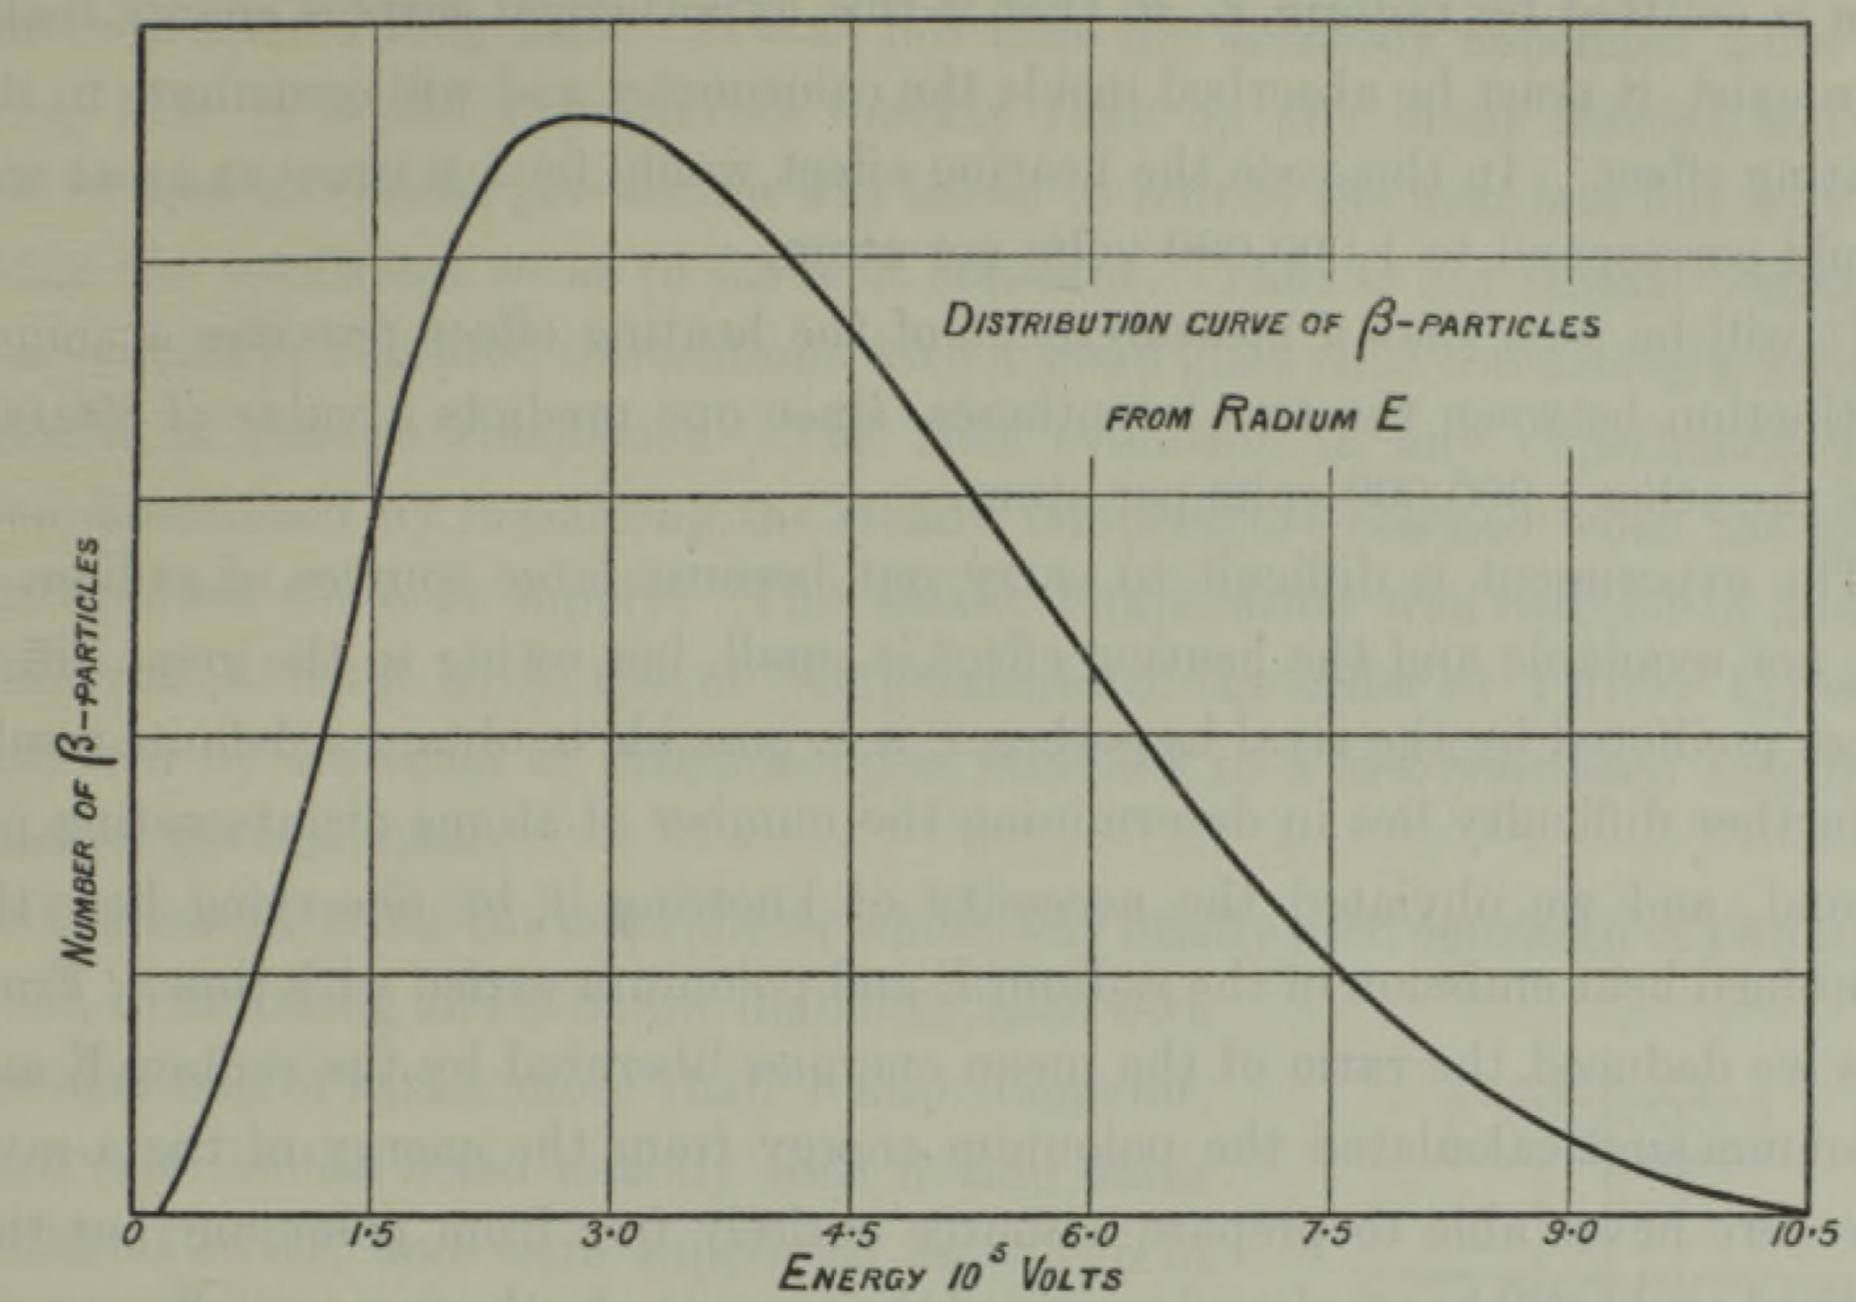
\includegraphics[width=0.6\textwidth]{Figures/BiSpectrum.png}
\caption[Continuous beta spectrum]{The continuous $\beta$ energy spectrum measured from $^{210}$Bi $\beta$-decay~\cite{bib:EandW}.}
\label{fig:BiSpectrum}
\end{figure}    
    
    Soon after the discovery of neutron, Fermi developed his theory of beta decay in 1934~\cite{bib:Fermi}, where the weak interaction was theorized. 
    In Fermi's theory of beta decay, neutrino was incorporated as a massless daughter particle that carries away part of the energy of a neutron beta decay:
    \begin{equation}\label{eq1.1}
        n \rightarrow p + e^- + \nu,
    \end{equation}
    where $\nu$ was named as neutrino for the first time.
    The neutrino generated in this process was later found to be \nuebar (electron antineutrino) to conserve lepton number in this process.

\Section{The Discovery of Neutrinos}
\label{Ch1Sec2}

    Though Pauli, when proposed neutrino's existence, stated it was a particle that \textit{cannot be detected}.
    The discovery of weak interaction found neutrino can interact with other particles by exchanging W or Z bosons.
    Among many types of neutrino-nucleon and -lepton interaction, neutrino can interact the similar way it is generated in $\beta$-decay:
    \begin{equation}
        \label{eq:IBD}
        \nuebar + p \rightarrow n + e^+,
    \end{equation}
    which is named as inverse beta decay (IBD), a quasielastic charged-current reaction between \nuebar and proton by exchanging a W boson.
    The cross-section of IBD reaction is estimated in the order of $\sim 10^{-43}\frac{p_eE_e}{\text{MeV}^2}$~(cm$^2$)~\cite{bib:IBDXsection}, where $p_e$ and $E_e$ are momentum and energy of positron produced.
    Such a rare interaction rate brought great challenge in neutrino detection that requires both high neutrino production from the source and huge amount of proton in the detector.
    
    In 1956, Cowan and Reines discovered neutrino through the detection of IBD~\cite{bib:CowanReines}.
    The neutrinos detected was \nuebar produced from the $\beta$-decay of daughter isotopes of the nuclear fission reactor at Savannah River plant.
    To detect the IBD signals, two target tanks filled with $^{108}$Cd loaded water were deployed in the two gaps made by three vertically aligned liquid scintillator (LS) detector.
    The signature of IBD process was the time coincidence between the positron and neutron produced in the reaction.
    When a proton in the water tank is hit by \nuebar, the produced positron will annihilate into a pair of 0.511~MeV $\gamma$, and the neutron is largely captured by $^{108}$Cd within 5~\textmu s, emitting reactor $\gamma$s with total energy from 3~MeV to 10~MeV.
    The $\gamma$s in the LS generate scintillation photons that are eventually collected by the 110 photomultiplier tubes (PMTs) in each LS detector. 
    By detecting $\gamma$ ray from the target tanks with time coincidence, the Cowan and Reines experiment collected 1013 \nuebar events in 900~hours reactor-on data acquisition.
    
    The conservation of lepton number with flavor requires $\beta$-decay only produce \nuebar.
    This conservation also forbids interactions like $\overline{\nu}_\mu + p \rightarrow n + e^+$, meaning ${\nu}_\mu$'s (muon neutrino) nucleon interaction cannot produce electron~\cite{bib:Ponte1959, bib:Schwartz}.
    In 1962, Schwartz, Lederman, and Steinberger induced high energy $\nu_\mu/\overline{\nu}_\mu$ produced from the decay from accelerated $\pi^\pm$~\cite{bib:numuDiscovery}.
    With 10 tons spark chamber consisting of 90 aluminum plates, the experiment at Brookhaven National Laboratory is able to distinguish electron and muon produced from $\nu_\mu/\overline{\nu}_\mu$'s interaction with nucleons. 
    This experiment discovered $\nu_\mu$ by finding only $\mu^\pm$ was detected in the chamber and so distinguished neutrinos with different flavors.
    
    In 2000, the DONUT collaboration at Fermilab discovered $\nu_\tau$ (tau neutrino) mainly decayed from the accelerated $D_s^- \rightarrow \tau^- + \overline{\nu}_\tau$. 
    Since the discovery of $\nu_\tau$, the family of neutrinos in Standard Model has six members $\nu_e$, $\nu_\mu$, $\nu_\tau$, and their antiparticles.
    
\Section{Observation of Neutrino Oscillation}
    
    Fermi also stated the neutrino being either massless or extremely light in his study of $\beta$-decay~\cite{bib:Fermi}.
    Following Yang and Lee's discussion of parity conservation question~\cite{bib:YangLee}, and Wu discovered that weak interaction violates parity symmetry by observing $\beta$ momentum direction preference from the $\beta$-decay of polarized $^{60}$Co~\cite{bib:Wu}.
    The parity violation of $\beta$-decay restricts the neutrino helicity being only left handed (and antineutrino helicity being only right handed).
    Therefore, massless neutrino and antineutrino is seemingly preferred in nature to obey the proper representation of the Lorentz group.
    The Standard Model was built with the assumption of massless neutrino.
    However, the experimental observation of neutrino oscillation proved neutrino having nonzero masses.

    The research of the oscillating neutrino began from the discovery of solar neutrino problem. 
    In 1968, Davis \textit{et al.} organized the solar neutrino experiment aiming to detect $\nu_e$ from nuclear fission reaction in the sun~\cite{bib:davis}.
    This experiment uses a target containing 390000 liters of C$_2$Cl$_4$ in the Homestake mine to detect the appearance of $^{37}$Ar in the $^{37}$Cl($\nu_e$, $e^-$)$^{37}$Ar reaction.
    The solar neutrino problem arose when the measured flux of $\nu_e$ is one third as predicted by the Standard Solar Model.
    In the following decades, more solar neutrino flux measurement, including GALLEX~\cite{bib:GALLEX}, GNO~\cite{bib:GNO}, SAGE~\cite{bib:SAGE}, and Kamiokande~\cite{bib:kamioka1996}, observed less solar $\nu_e$ flux from expectation.
    Also, atmosphere neutrino measurements, the IMB~\cite{bib:IMB} and Kamiokande~\cite{bib:Kamioka1986} experiments, detected fewer atmosphere neutrino from prediction, which is referred as the \textit{atmosphere neutrino anomaly}.
    These deficits to theoretical models provided the experimental hints to neutrino oscillation. 
    
    The observation of neutrino oscillation was first achieved by the Super-K experiment~\cite{bib:SuperK} in 1998. 
    Using a water Cherenkov detector with 50000 tons of pure and 13000 PMTs, the experiment observed the atmosphere $\nu_\mu$ flux difference among a large variety of zenith angle shown in Figure~\ref{fig:SuperK}.
    The difference of atmosphere neutrino flux was caused by a the $\nu_\mu$s oscillated into other flavors when traveling through the earth until being collected in the detector.
    
\begin{figure}[h!]
\centering
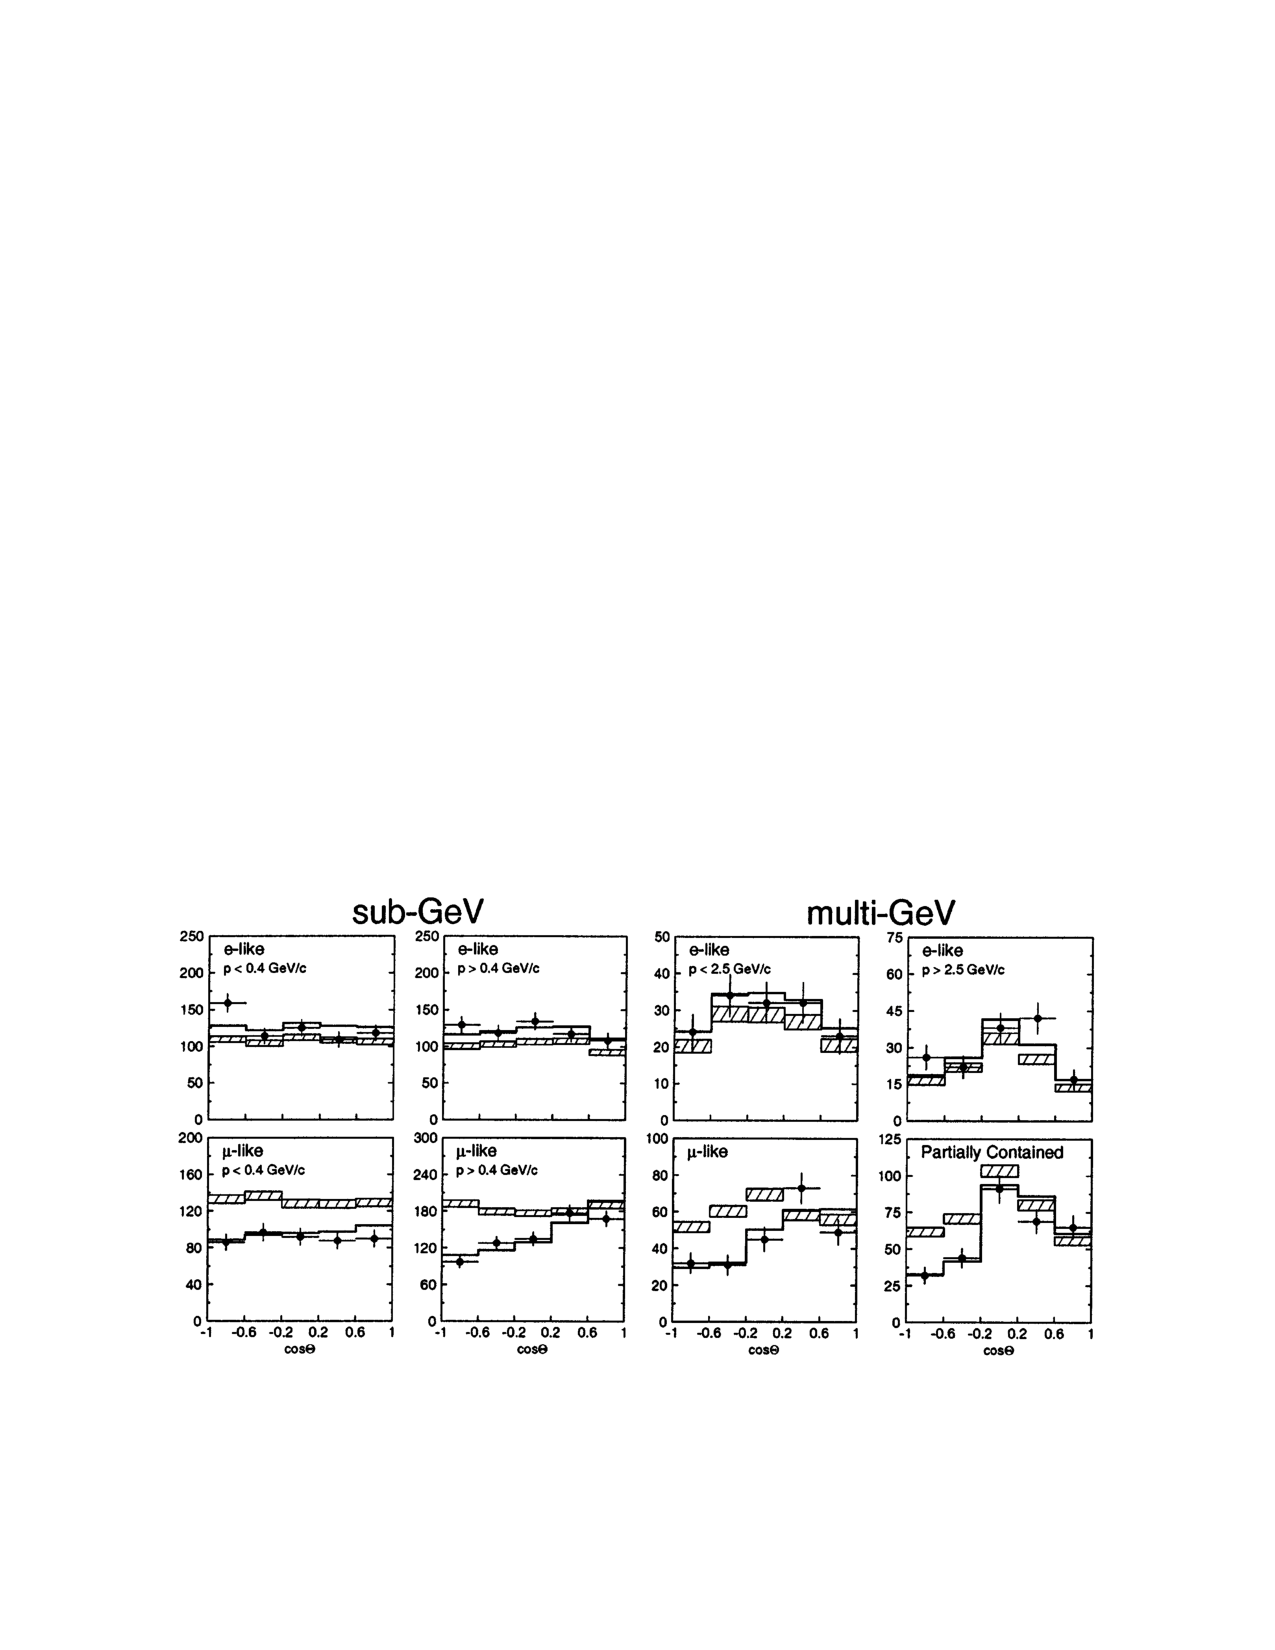
\includegraphics[width=0.95\textwidth]{Figures/SuperK.pdf}
\caption[Atmosphere neutrino oscillation]{The flux of $e$-like and $\mu$-like events measured by the Super-K experiment~\cite{bib:SuperK}. The $\mu$-like, correlated to number of $\nu_\mu$ collected, varies significantly with respect to zenith angle. The solid line (shaded region) represents the Monte-Carlo (MC) with (without) the model of neutrino oscillation.  }
\label{fig:SuperK}
\end{figure}

    In 2001, SNO experiment~\cite{bib:SNO} deployed heavy water Cherenkov detector that is able to detect charged-current (CC), neutral-current (NC) and elastic scattering (ES) to detect solar neutrinos of all flavors in comparison with $\nu_e$s.
    If neutrino oscillates among flavors, the solar $\nu_e$ will oscillates into other flavors while conserve the  neutrino flux of all flavors.
    As shown in Figure~\ref{fig:sno}, the experiment is able to confirm solar neutrino oscillation by comparing neutrino flux measured with different scattering mode.
    Super-K and SNO experiments provided solid experimental evidences of neutrino oscillation and resolved the solar neutrino problem and atmosphere neutrino anomaly.
    
\begin{figure}[h!]
\centering
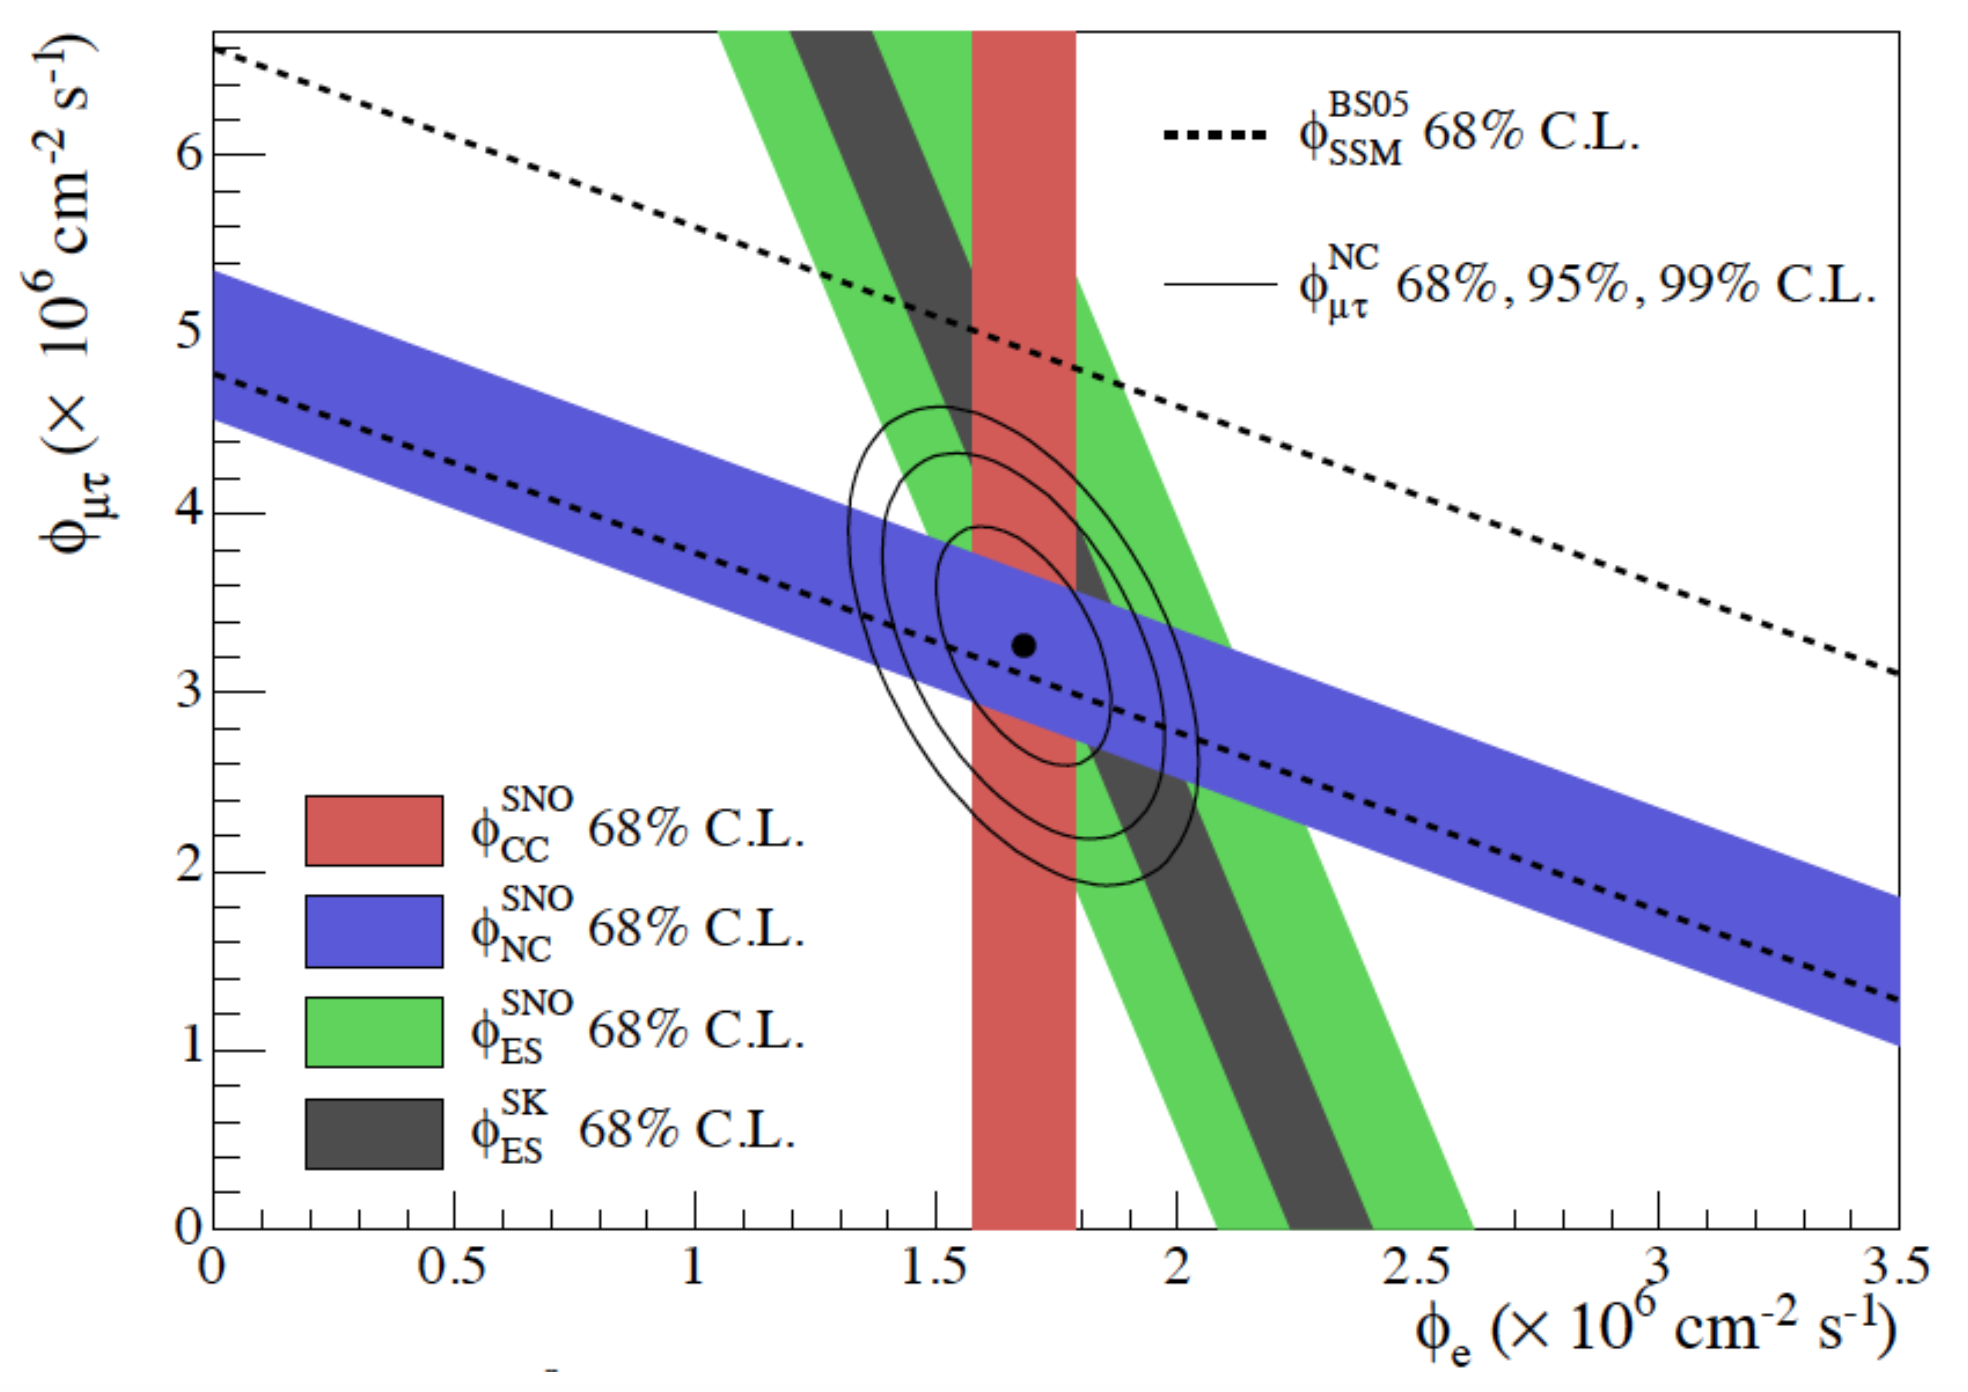
\includegraphics[width=0.6\textwidth]{Figures/sno.png}
\caption[Solar neutrino oscillation]{The flux of different scattering modes of solar neutrinos measured by SNO. The all-flavor flux (NC and ES) agreed. The day-night flux indicates $\nu_e$'s oscillation into other flavors. }
\label{fig:sno}
\end{figure}

\Section{Massive Neutrino}
    
    The discovery of neutrino oscillation implies massive neutrino.
    Although the natural origin of neutrino mass is undetermined, neutrinos can obtain mass through the Higgs mechanism similar to other leptons. 
    Under the assumption of neutrino being Dirac fermion (particle distinct from antiparticle), Higgs-lepton Yukawa Lagragian term can be written as
\begin{equation}\label{eq4}
\mathscr{L}_H = -\left(\frac{v+H}{\sqrt{2}}\right)\left[\overline{l'_L}Y'^{l}l'_R +\overline{\nu'_L}Y'^{\nu}\nu'_R\right],
\end{equation}
    where $v$ is the Higgs vacuum expectation value (VEV), $H$ is the higgs field, and $Y$ is the Yukawa coupling matrix. 
    The matrix can be diagonalized with the unitary matrice $V_L$ and $V_R$.
\begin{equation}\label{eq5}
V^\dagger_LY'V_R = Y,\   \ \textrm{with} \   \ Y_{kj} = y_k\delta_{kj} \   \ (k,j = 1,2,3),
\end{equation}
    where $y_k$ is the eigenvalue of Yukawa coupling matrix. The neutrino mass states array with the three-generation mixing is defined as:
\begin{equation}\label{eq6}
\nu'_L \rightarrow V^{\nu\dagger}_L\nu'_L = \left( \begin{array}{c}
\nu_{1L} \\
\nu_{2L} \\
\nu_{3L} \\
\end{array} \right) \   \ \text{and} \   \ \nu'_R \rightarrow V^{\nu\dagger}_R\nu'_R = \left( \begin{array}{c}
\nu_{1R} \\
\nu_{2R} \\
\nu_{3R} \\
\end{array} \right).
\end{equation}
    Consider $l_\alpha = l_{\alpha L} + l_{\alpha R}$ and $\nu_k = \nu_{kL} + \nu_{kR}$, the Lagrangian can be rewritten as
\begin{equation}\label{eq7}
\begin{aligned}
\mathscr{L}_H & = -\left(\frac{v+H}{\sqrt{2}}\right)\left[ \sum\limits_{\alpha = e, \mu, \tau} y_{\alpha}^l\overline{l_{\alpha L}}l_{\alpha R} + \sum\limits_{k = 1, 2, 3}y_k^\nu \overline{\nu_{kL}}\nu_{kR} \right] \\
& = - \sum\limits_{\alpha = e, \mu, \tau} \frac{y_\alpha^l v}{\sqrt{2}}\overline{l_{\alpha}}l_{\alpha} - \sum\limits_{k = 1, 2, 3} \frac{y_k^\nu v}{\sqrt{2}} \overline{\nu_{k}}\nu_{k} - \sum\limits_{\alpha = e, \mu, \tau} \frac{y_\alpha^l}{\sqrt{2}}\overline{l_{\alpha}}l_{\alpha}H - \sum\limits_{k = 1, 2, 3} \frac{y_k^\nu}{\sqrt{2}} \overline{\nu_{k}}\nu_{k}H.
\end{aligned}
\end{equation}
    Since $\nu_k = \nu_{kL} + \nu_{kR}$, the Dirac mass term of neutrino is simplified as
\begin{equation}\label{eq8}
\begin{aligned}
    \mathscr{L}^D_{mass} &= -\sum\limits_{k = 1, 2, 3} m_k^D\overline{\nu_{k}}\nu_{k} + \textrm{H.c.} \\
    & = -\sum\limits_{k = 1, 2, 3}m_k^D(\overline{\nu_{kL}}\nu_{kR} + \overline{\nu_{kR}}\nu_{kL}) + \textrm{H.c.},
\end{aligned}
\end{equation}
    where the Dirac mass of neutrino $m_k^D = \frac{y_k^\nu v}{\sqrt{2}}$ and $\overline{\nu_{kL}}\nu_{kL} = \overline{\nu_{kR}}\nu_{kR} = 0$.
    This mechanism for neutrino to obtain mass involves right handed neutrino $\nu_R$, also refered \textit{sterile neutrino} for its incapability of interacting under the parity violating weak force.
    
    Because of its neutral nature, neutrino is a candidate Majorana fermion (the particle is its own antiparticle).
    The 
    Under this condition, the neutrino field is
    \begin{equation}\label{eq9}
        \nu = \nu_L + \mathcal{C}\overline{\nu_L}^T,
    \end{equation}
    where neutrino $\mathcal{C}$ is charge conjugate matrix.
    The Majorana mass term of the lepton Lagrangian can be written as 
    \begin{equation}\label{eq10}
\begin{aligned}
    \mathscr{L}^M_{mass} &= \frac{1}{2}m_L{\nu_{L}^T} \mathcal{C}^\dagger \nu_{L} + \textrm{H.c.},
\end{aligned}
\end{equation}
    in which $m^L$ is the left handed Majorana mass.
    Majorana mass term of neutrino avoided the assumption of right handed neutrino.
    
    However, it is theoretically allowed that both right handed neutrino and Majorana neutrino can exist in theory. 
    Thus, a more general neutrino mass term for single neutrino scenario is defined as 
    \begin{equation}
    \label{eq11}
    \begin{aligned}
    \mathscr{L}_{mass}^{D+M} &= - m_D(\overline{\nu_{L}}\nu_{R} + \overline{\nu_{R}}\nu_{L}) + \frac{1}{2}m_L{\nu_{L}^T} \mathcal{C}^\dagger \nu_{L} + \frac{1}{2}m_R{\nu_{R}^T} \mathcal{C}^\dagger \nu_{R} + \textrm{H.c.} \\
    & = \frac{1}{2}(\begin{array}{cc}
    \overline{\nu^C_L} & \overline{\nu_R} \end{array}) 
    \left(\begin{array}{cc}
    m_L & m_D \\
    m_D & m_R
    \end{array}\right)
    \left(\begin{array}{c}
    \nu_L \\
    \nu_R^C
    \end{array}\right) + \textrm{H.c.}.
    \end{aligned}
    \end{equation}
    In a special case, when $m^D \ll m_R$ and $m_L = 0$, Equation~\ref{eq11} can be diagonalized as
    \begin{equation}
    \label{eq12}
    \mathscr{L}_{mass}^{D+M}  = \frac{1}{2}(\begin{array}{cc}
    \overline{\nu^1} & \overline{\nu_2} \end{array}) 
    \left(\begin{array}{cc}
    \frac{m_D^2}{m_R} &  \\
     & m_R
    \end{array}\right)
    \left(\begin{array}{c}
    \nu_1 \\
    \nu_2
    \end{array}\right) + \textrm{H.c.}
    \end{equation}
    This is called Type-I seesaw mechanism, a possible explanation of the tiny mass of left handed neutrino.

\Section{Theory of Neutrino Oscillation}
    
    The theoretical study of neutrino oscillation started in 1950s.
    Pontecorvo~\cite{bib:Pontecorvo1957, bib:Pontecorvo1957qd} proposed neutrino oscillation inspired from observation of $K^0 \leftrightarrow \overline{K}^0$ oscillation.
    In 1967, Maki, Nakagawa, and Sakata discussed the theory of two-neutrino fla mixing~\cite{bib:Maki1962}.
    Later in 1969, Gribov and Pontecorvo explicitly developed theory of neutrino oscillation with mass state mixing~\cite{bib:GRIBOV1969}. 
    By allowing massive neutrino, the neutrino portion of the Lagrangian can be expressed analogous to other massive particles.
\begin{equation}
\label{eq13}
\mathscr{L}_\nu = -\left[m^\nu_\alpha\overline{\nu_\alpha}\nu_\alpha + m^\nu_\beta\overline{\nu_\beta}\nu_\beta + m^\nu_\alpha m^\nu_\beta(\overline{\nu_\alpha}\nu_\beta + \overline{\nu_\beta}\nu_\alpha) \right] \   \ (\alpha, \beta = e, \mu, \tau).
\end{equation}
    This equation can be rewritten as
\begin{equation}
\label{eq14}
\mathscr{L}_\nu = \overline{\nu}_\alpha\mathcal{M}^\nu\nu_\beta.
\end{equation}
    where the $\mathcal{M}'^\nu$ is can be diagonalized. 
    The conversion between the two matrix expressions above transforms the flavor states of neutrino to mass states by a unitary matrix $U$:
\begin{equation}\label{eq15}
\left(\begin{array}{c}
\nu_\alpha \\
\nu_\beta
\end{array}\right) = \left(\begin{array}{cc}
\cos\theta & \sin\theta \\
-\sin\theta & \cos\theta
\end{array}\right)\left(\begin{array}{c}
\nu_k \\
\nu_l
\end{array}\right).
\end{equation}

    When $\theta \neq 0$, this transformation is a two generation mixing of neutrino mass eigenstates in the neutrino flavors, meaning neutrino's flavors are not orthogonal to its mass eigenstates.
    This matrix can be expanded to three neutrino mixing with the unitary matrix $U_{PMNS}$, the Pontecorvo-Maki-Nakagawa-Sakata (PMNS) matrix, a neutrino equivalent to the CKM mixing of quarks. 
    In addition to the 3x3 angle transformation, the matrix also includes the CP-violation phase factor $\delta_{CP}$ and a diagonal mixing matrix of Majorana neutrino term $D_\textrm{Majorana}$. 
    The three generation neutrino mixing matrix is 
    \begin{equation}\label{eq16}
    \begin{aligned}
    U & =  U_{PMNS}\cdot D_\textrm{Majorana} \\
    & =  \left(\begin{array}{ccc}
    U_{e1} & U_{e2} & U_{e3} \\
    U_{\mu 1} & U_{\mu 2} & U_{\mu 3} \\
    U_{\tau 1} & U_{\tau 2} & U_{\tau 3}
    \end{array}\right) \\
    & = \left(\begin{array}{ccc}
    1   &   &  \\
        &   c_{23}  & s_{23} \\
        &   -s_{23} & c_{23}
    \end{array}\right) 
    \left(\begin{array}{ccc}
    c_{13}  &   & s_{13}e^{-i\delta_{CP}} \\
        & 1 &  \\
    -s_{13}e^{i\delta_{CP}}  &   & c_{13}
    \end{array}\right) 
    \left(\begin{array}{ccc}
    c_{12}  & s_{12}  &  \\
    -s_{12} & c_{12} &  \\
        &   & 1
    \end{array}\right)  \\
    &\cdot\left( \begin{array}{ccc}
    e^{i\xi_1/2} & & \\
    & e^{-i\xi_1/2} & \\
    & & 1 \\
    \end{array}\right)
    \end{aligned}
    \end{equation}

    Hence, the flavor eigenstates of the neutrino can be described as a sum of the mass states with a matrix element form $U_{PMNS}$:
    \begin{equation}\label{eq17}
    |\nu_\alpha\rangle = \sum\limits_{k=1,2,3} U^*_{\alpha k}|\nu_k\rangle.
    \end{equation}
    Using the time-dependent Schr{\"o}dinger equation, the time evolution of neutrino flavor is expressed as
    \begin{equation}
    \label{eq18}
    |\nu_\alpha(t)\rangle = \sum\limits_{k=1,2,3} U^*_{\alpha k}e^{-i(E_k)t}|\nu_k\rangle.
    \end{equation}
    Therefore, the probability of a neutrino oscillating from one flavor to the other is
    \begin{equation}\label{eq19}
    \begin{aligned}
    P_{\nu_\alpha\rightarrow\nu_\beta} & =|\langle\nu_\beta|\nu_\alpha(t)\rangle|^2 \\
    & =\sum\limits_{k,j}U^*_{\alpha k} U_{\beta k} U_{\alpha j} U^*_{\beta j} e^{-i(E_k-E_j)t} \\
    & =\sum\limits_{k,j}U^*_{\alpha k} U_{\beta k} U_{\alpha j} U^*_{\beta j}\exp\left(-i\frac{\Delta m^2_{kj}L}{2E}\right),
    \end{aligned}
    \end{equation}
    where $\Delta m_{kj}^2 =m_k^2 - m_j^2$, $L$ is the neutrino travelling distance, and $E$ is the kinetic energy of neutrino.
    This equation proves a nonzero neutrino oscillation probability requires the mixing of massive neutrino.
    It also shows that the phase of the neutrino oscillation depends on the factor $\frac{\Delta m^2_{kj}L}{2E}$ explaining both the solar neutrino problem and the atmosphere neutrino anomaly. 
    
    The probability Equation~\ref{eq19} can be generalized to any neutrino flavor transition in oscillation as
\begin{equation}\label{eq20}
\begin{aligned}
	P_{\nu_\alpha\rightarrow\nu_\beta} = \delta_{\alpha\beta} & -  4 \sum\limits_{k>j}\textbf{Re} \left[ U^*_{\alpha k} U_{\beta k} U_{\alpha j} U^*_{\beta j}\right]\sin^2\left(\frac{\Delta m^2_{kj}L}{4E}\right) \\
	 & \pm 2 \sum\limits_{k>j} \textbf{Im} \left[
	 U^*_{\alpha k} U_{\beta k} U_{\alpha j} U^*_{\beta j}\right]\sin\left(-i\frac{\Delta m^2_{kj}L}{2E}\right).
\end{aligned}
\end{equation}
    The imaginary component is positive for neutrinos, and negative for antineutrinos. 
    In two neutrino mixing, Equation~\ref{eq19} can be simplified as
    \begin{equation}\label{eq21}
    \begin{aligned}
    P_{\nu_\alpha\rightarrow\nu_\beta} & = \sin^2{2\theta}\sin^2\left( 1.27\frac{\Delta m^2L}{E} \right)
    \end{aligned}
    \end{equation}
    to calculate the appearance probability of one flavor during neutrino oscillation in vacuum.
    Similarly, the survival probability of the original neutrino flavor can be written as 
    \begin{equation}\label{eq22}
    \begin{aligned}
    P_{\nu_\alpha\rightarrow\nu_\alpha} & = 1- \sin^2{2\theta}\sin^2\left( 1.27\frac{\Delta m^2L}{E} \right).
    \end{aligned}
    \end{equation}
    The probability equations (2.21) and (2.22) are frequently used as theoretical tool in neutrino oscillation experiments to calculate their oscillation models.

\Section{Measurements of Neutrino Oscillation}
    
    Experimental efforts have been made in the past two decades to determine the key neutrino oscillation parameters.
    By flux of survived and appeared neutrino during oscillation through varieties of baseline, the experiments is able to measure $\theta_{23}$, $\theta_{13}$, $\theta_{12}$, $\Delta m^2_{21}$ and $|\Delta m^2_{31}|$. 
    The $\theta_{12}$ and $\Delta m^2_{21}$ determined by the  phenomenological analyses of solar neutrino flux measurements~\cite{bib:SNOPRC} and KamLAND reactor \nuebar oscillation measurement~\cite{bib:KamLAND03}.
    By measuring the disappearance of $\nu_\mu$ and $\overline{\nu}_\mu$ in atmosphere neutrino experiments~\cite{bib:MACRO,bib:Soudan2}, long baseline accelerator neutrino experiments~\cite{bib:k2k,bib:MINOS,bib:t2k,bib:nova}, and neutrino telescope observation~\cite{bib:ANTARES, bib:ICEosc}, $\theta_{23}$ and $|\Delta m^2_{31(32)}|$ is measured.
    The $\theta_{13}$ is thoroughly measured through the short baseline reactor $\nuebar$ flux measurements~\cite{bib:DYBosc,bib:RENO,bib:DBChooz}, which is decribed in detail in Chapter~2.
    The results of the neutrino mass mixing parameters are shown in Table~\ref{tab:1.1}.
    \begin{table}[h]
    \centering
    \begin{tabular}{lll}
    \hline
    \hline
    Parameters                  & Value             & 3-$\sigma$    \\ \hline
    $\sin^2(\theta _{12})$      & 0.297             & $0.250 - 0.354$
    \\ \hline
    $\sin^2(\theta _{23})$      & 0.425 (normal)    & $0.381 - 0.615$ \\
                                & 0.589 (inverted)  & $0.384 - 0.636$ \\ \hline
    $\sin^2(\theta_{13})$       & 0.0215 (normal)   & $0.0190 - 0.0240$ \\   
                                & 0.0216 (inverted) & $0.0190 - 0.0242$ \\ \hline
    $\Delta m^ 2_{21} (10^{-5}\textrm{eV}^2) $      & 7.57              & $6.93 - 7.96$ \\ \hline
    $|\Delta m^ 2_{31}| (10^{-3}\textrm{eV}^2) $    & 2.56 (normal)     & $2.45 - 2.69$\\
                                & 2.54 (inverted)   & $2.42 - 2.66$\\
    \hline\hline
    \end{tabular}
    \caption[Neutrino Oscillation Parameters]{Measured parameters of neutrino oscillation~\cite{bib:PDG}.}
    \label{tab:1.1}
    \end{table}
    
\Section{Future Tasks of Neutrino Experiments}
\label{ch1sec7}
    
    The properties of massive neutrino are of main interest of future experimental research, for it being the first solid experimental evidence of physics beyond standard model.
    
    The studies of Dirac or Majorana nature of neutrino are organized worldwide. 
    If neutrino less double $\beta$-decay ($0\nu\beta\beta$) is observed, neutrino can be determined as the first Majorana fermion ever detected.
    
    Several experiments are directly measuring the neutrino mass by searching for the end of $\beta$ spectrum with very high energy resolution. 
    
    The neutrino mass hierarchy, lepton CP violation and light sterile neutrino searching need more precise measurements of neutrino oscillation from different neutrino sources in different baselines. 
    These studies involve precise ratio of different transitions in oscillation, high resolution energy spectrum measurement, neutrino-antineutrino oscillation ratio, and very short baseline oscillation measurements.

\Chapter{Reactor Antineutrino}
\label{Ch2}

    Neutrinos can be categorized by the source they are generated from, including natural sources and artificial sources.
    The solar neutrino, relic neutrino, supernova neutrino, earth neutrino and atmosphere neutrino are neutrinos generated by natural cosmological or radioactive sources.
    The reactor antineutrino, henceforth mentioned as \textit{reactor neutrino}, and accelerator neutrino are man-made.
    
    Reactor neutrino experiments have the advantages of
    \begin{itemize}
        \item Relatively high statistics;
        \item Easy-to-control baseline;
        \item Relatively narrow range of neutrino energy.
    \end{itemize}
    Thus, reactor neutrino experiments have played irreplaceable role in the history neutrino detection and oscillation measurements.
    
\Section{The Flux and Spectrum of Reactor Neutrino}
    
    Reactor neutrino is \nuebar generated through $\beta$-decay of the daughter nuclei of nuclear fission process.
    Since the discoveries of lepton number conservation and neutrino flavors, the Equation~\ref{eq1.1} is rewritten as a neutron decay producing \nuebar,
    \begin{equation}\label{eq2.1}
        n \rightarrow p + e^- + \nuebar.
    \end{equation}
    The chain reaction of the nuclear reactor produces a great variety of branches fission product isotopes that mainly release their energy through the beta decay.
    One fission reaction naturally emits multiple neutrinos, each with kinetic energy mainly in 0~MeV to 10~MeV.
    
    The fission reaction of reactors that has been observed to detect neutrino are \Ulow dominated, with other main isotopes including $^{238}$U, $^{239}$Pu and $^{241}$Pu.
    The spectrum of reactor neutrino can be expressed as
    \begin{equation}\label{eq2.2}
        S(E_\nu) = \frac{W_{reactor}}{\sum_i \frac{f_i}{F}e_i}\sum_i\frac{f_i}{F}(\frac{dN_i}{dE_\nu}),
    \end{equation}
    where $W_reactor$ is the thermal power of the reactor, $i$ is each of the four fission isotopes, $f_i/F$ is the relative fraction of each isotope, $e_i$ is energy per fission, and 
    \begin{equation}
        \frac{dN_i}{dE_\nu} = \sum_n Y_n(t)(\sum_j b_{n,j}\cdot P(E_\nu, E_0^{n,j})),
        \label{eq:23}
    \end{equation}
    which is the summed energy spectrum of each fission isotope.
    In Equation~\ref{eq:23}, $Y_n(t)$ is cumulative fission yield, $b_{n,j}$ are the $\beta$-branches, and $P(E_\nu, E_0^{n,j})$ is the spectrum of each branch.
    A typical reactor has thousands of $\beta$-decay branches. 
    By adding the neutrino spectra of these branches, one can predict the spectrum of neutrino generated from a reactor, as an example showed in Figure~\ref{fig:2.1},
    \begin{figure}[h!]\label{fig:2.1}
    \centering
    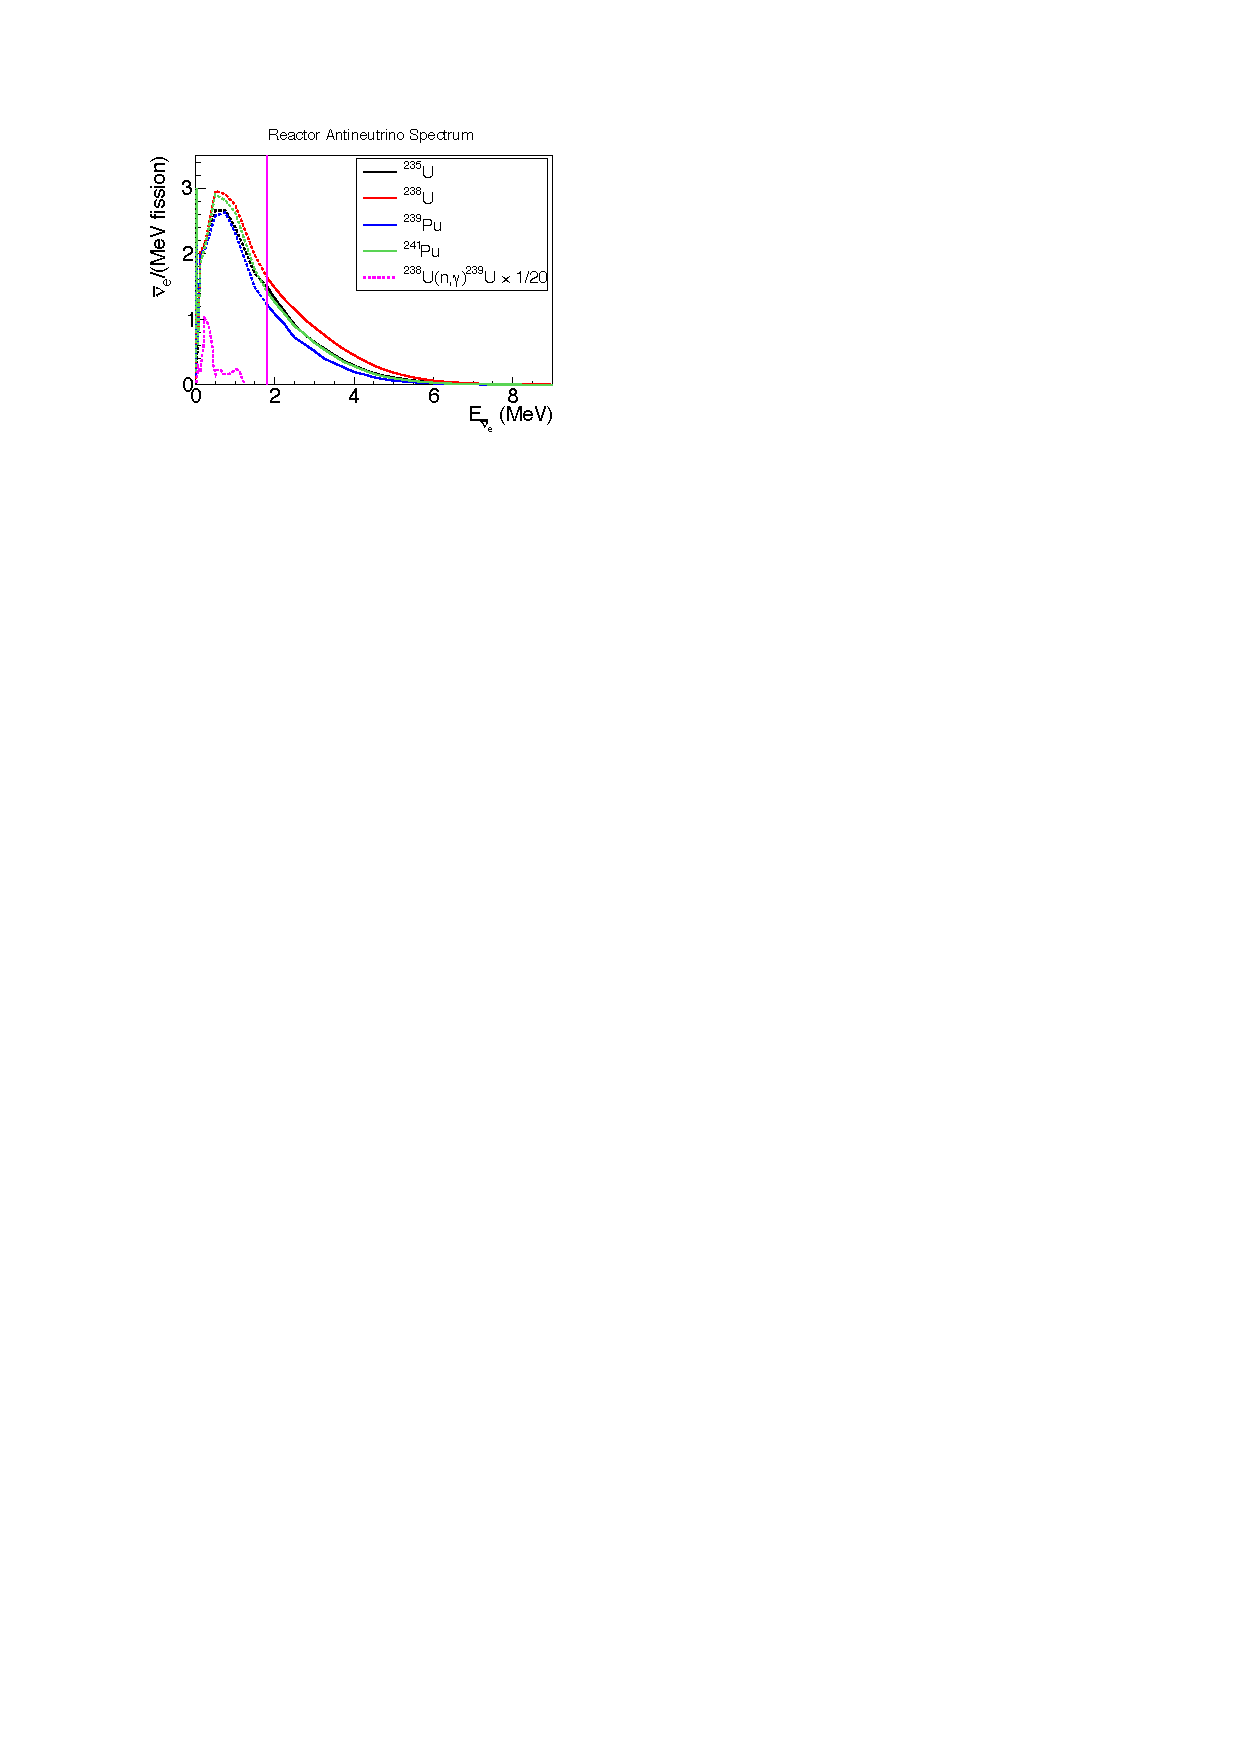
\includegraphics[width=0.5\textwidth]{Figures/RxNeutrinoSpec.pdf}
    \caption[Reactor neutrino spectrum]{An illustration of a commercial reactor neutrino spectrum prediction~\cite{bib:Qian2019}.}
    \end{figure}  

    Reactor neutrino detection experiments rely on the detection of IBD process showed in Equation~\ref{eq1.1}.
    Be cause of the mass difference between neutron and proton, the neutrino energy $E_\nu$ must be above a threshold to trigger the IBD process, as
    \begin{equation}\label{eq2.4}
    E_\nu \ge \frac{(m_n+m+e)^2 - m_p}{2m_p} \simeq 1.806 \textrm{MeV}.
    \end{equation}
    The kinectic energy of the IBD produced neutron $T_n$ is in keV scale.
    Thus, the $e^+$ total energy of IBD can be expressed as
    \begin{equation}\label{eq2.5}
    E_e = E_\nu - (m_n + T_n - m_p) \simeq E_\nu - 1.293 MeV.
    \end{equation}
    In IBD detector, the $e^+$ quickly annihilates with $e^-$ and emits two 0.511~MeV $\gamma$.
    The visible energy of IBD produced $e+$ in an ideal detector is 
    \begin{equation}\label{eq2.6}
    E_{vis} = \simeq E_\nu - 0.782 MeV,
    \end{equation}
    which is a useful experimental conversion for measurement \nuebar energy measurement by measuring the positron energy. 
    The cross-section of the IBD interaction is dependent on the neutrino energy and can be expressed as a function of positron energy
    \begin{equation}\label{eq2.7}
    \sigma_{IBD} \simeq \frac{2\pi^2}{\tau_n m_e^5 f }E_eP_e = 10^{-43}\cdot \frac{E_ep_e}{\textrm{MeV}}\cdot(\frac{\tau_n}{886\textrm{s}})^{-1} \textrm{cm}^2,
    \end{equation} 
    where $\tau$ is neutron life time and $f$ is a phase space integral factor.
    Based on the theoretical neutrino spectrum (Equation~\ref{eq2.2}) and IBD cross-section (Equation~\ref{eq2.7}), an reactor neutrino experiment can expect the measured spectrum and flux as shown in Figure~\ref{fig:2.2}.
    \begin{figure}[h!]
    \centering
    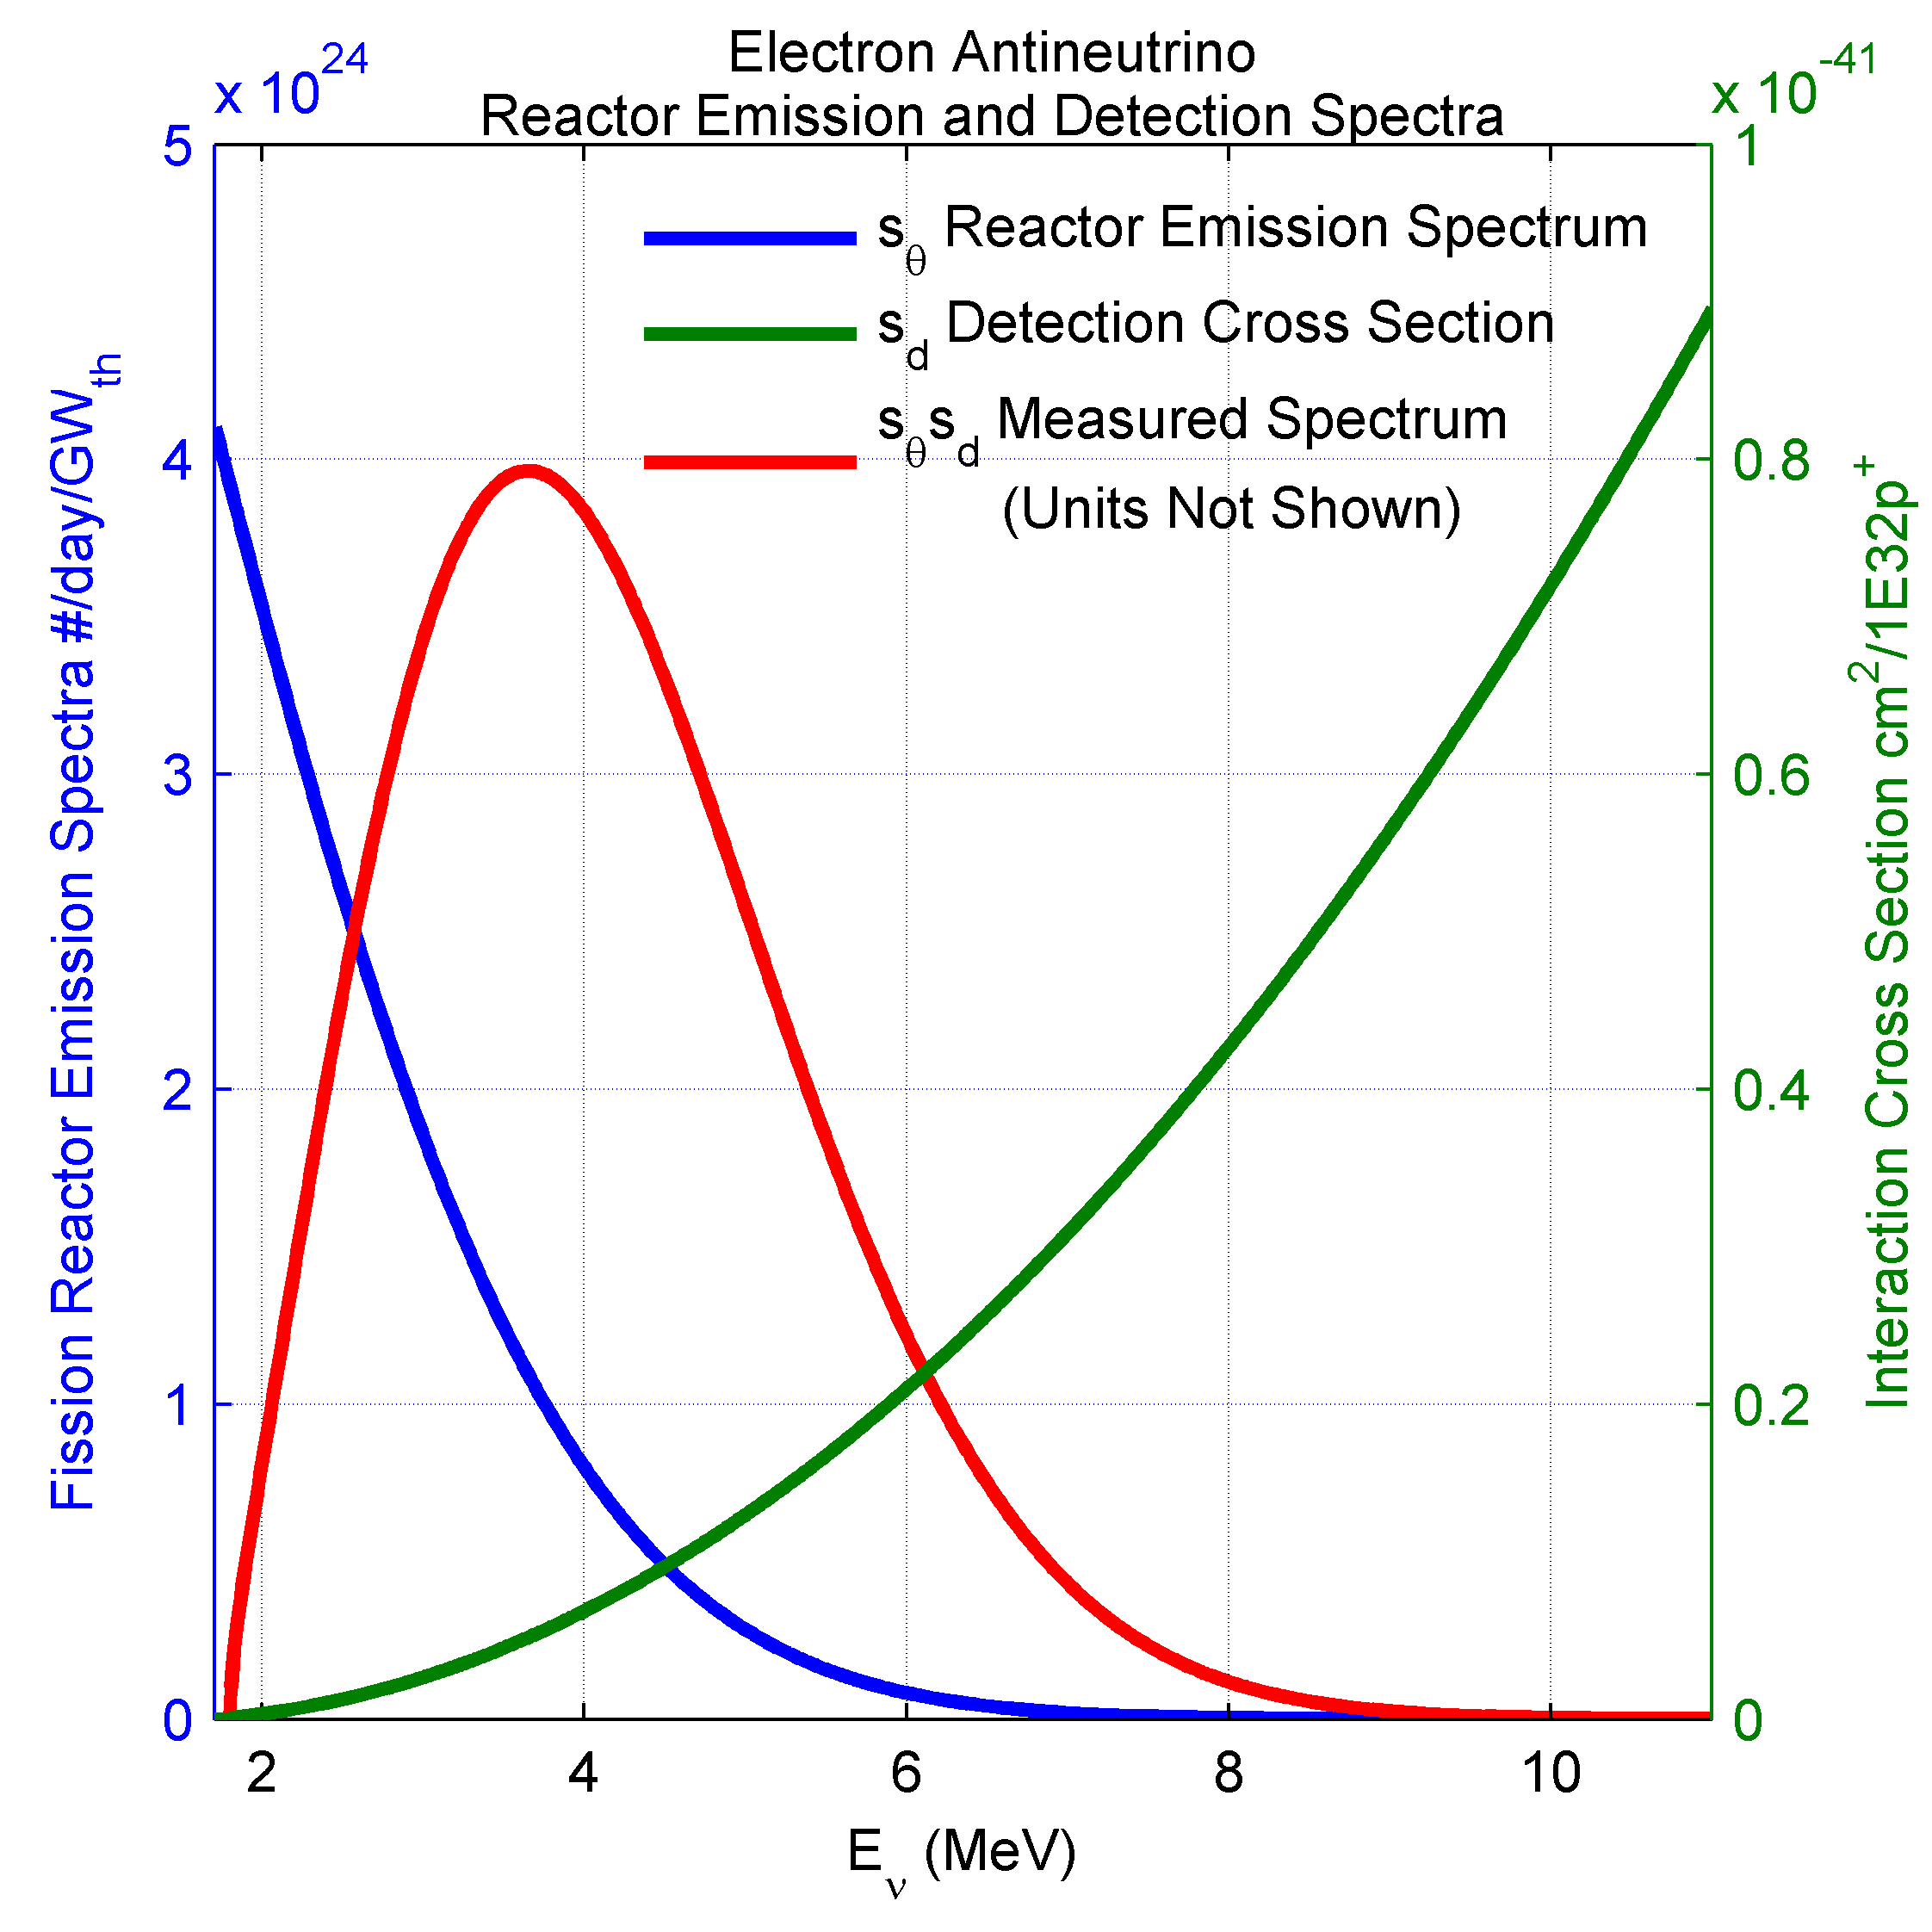
\includegraphics[width=0.6\textwidth]{Figures/twoXsections.png}
    \caption[Detected neutrino spectrum]{An illustration~\cite{bib:Jocher} of the detected neutrino energy spectrum in a reactor experiment. 
    The detected spectrum is the multiplication of the emitted neutrino spectrum and IBD cross-section.}
    \label{fig:2.2}
    \end{figure}      
    
    Reactor neutrino researches have interest of testing the success of nuclear and particle physics by compare experimental measurements of reactor neutrino flux and spectra to the predictions.
    There are two methods to predict the absolute neutrino spectrum of a nuclear reactor:
    \begin{itemize}
        \item \textbf{The \textit{ab initio} method} Neutrino spectrum is calculated by Equation~\ref{eq2.2} and \ref{eq:23}. 
        Where the ratio and the end point energy of each branch is extracted from data in nuclear databases.
        The predicted neutron spectrum is the sum of the calculated $\beta$-spectrum involving theoretical corrections. 
        The neutrino spectrum of $^{238}$U is originally predicted in this way~\cite{bib:vogel}.
        \item \textbf{$\beta$-conversion method} Because the kinetic energy of proton is negligibly small, the total $\beta$-decay end point energy $E_0 \simeq E_\nu + E_e$.
        The neutrino spectrum can be deduced from the experimental measurement of $\beta$ energy from fission reactor. 
        In 1980s, the $^{235}$U, $^{239}$Pu, and $^{241}$Pu neutrino spectra was converted from the spectrum measurements of $\beta$ from the Institut Laue-Langevin (ILL) reactor~\cite{bib:ILL1982,bib:ILL1985,bib:ILL1989}.
        The conversion was made by fitting the measured $\beta$ spectrum with sum of tens of hypothetical $\beta$-decay branches, then converting the spectrum of each $\beta$ branch to neutrino spectrum with respect to the best-fit branch ratio.
    \end{itemize}
    The detailed theoretical approaches are described in Section 3 of this chapter. 
    
    Successful neutrino flux and spectrum prediction and measurement made it possible for reactor neutrino experiments to test nuclear model of fission reactors.

\Section{Historical Context of Reactor Neutrino Experiments}

    After neutrino's discovery through the detection by the Savannah reactor neutrino experiment~\cite{bib:CowanReines},
    a hint of $\nuebar$ oscillation was discovered by Reines \textit{et al} in 1980~\cite{bib:reines1980}.
    Their experiment found in unexpected ratio charged current and neutral current interaction with $2\sigma-3\sigma$, which suggests antineutrino oscillation.
    More reactor experiments were built to test \nuebar oscillation covering a big variety of baseline by comparing neutrino flux to the theoretical predictions or between different baselines, included in Table~\ref{tab:history}.
    \begin{table}[h]
    \centering
    \begin{tabular}{lllll}
    \hline
    Experiment  & Baseline   & Absolute Flux  & Relative Flux    & Reference   \\ 
    \hline
    ILL     & 8.76~m  & $0.955\pm 0.115$  &  & \cite{bib:kwon1981}  \\
    \hline
        & 37.9~m   & $1.018\pm 0.06$  &   &   \\
    G\"osgen  & 45.9~m  & $1.045\pm 0.06$  &   & \cite{bib:gosgen}  \\
        & 64.7~m    & $0.975\pm 0.06$  &   &   \\
    \hline
    Rovno     & 18.3~m to 25.3~m     & $0.964\pm 0.068$  &   & \cite{bib:Afonin1987}  \\
    \hline
    Krasnoyarsk     &  57~m to 231~m    & $0.99\pm 0.05$  & $0.86\pm 0.15$  &  \cite{bib:Vidyakin1994} \\
    \hline
        & 14~m & $0.988\pm 0.05$  &   &   \\
    Bugey   & 40~m  & $0.994\pm 0.05$  &   &  \cite{bib:Bugey} \\
        & 95~m  & $0.913\pm 0.13$  &   &   \\
    \hline
    Savannah River  &  18~m & $0.987\pm 0.038$ &    & \cite{bib:Greenwood1996} \\
        &4~m    & $1.055\pm 0.038$  &   &   \\
    \hline
    CHOOZ   & 1~km     & $1.01\pm 0.04$   &   & \cite{bib:chooz98, bib:Chooz99, bib:chooz03}  \\
    \hline
    Palo Verde   &  750~m to 890~m & $1.04\pm 0.09$ &   &  \cite{bib:palo01, bib:palo1999, bib:palo2000} \\
    \hline
    KamLAND & 80~km to 800~km  &  $0.658\pm 0.06$ &   & \cite{bib:kamland02, bib:kamland04}  \\
    \hline
    \end{tabular}
    \caption[Historical reactor oscillation experiments]{The historical reactor experiments searching for \nuebar oscillation in baseline from $\sim$10~m to $\sim$100~km.
    The experiments attempted to observe neutrino oscillation through \nuebar disappearance.
    The commonly used methods are to compare the observed neutrino flux to the expected flux, or to compare the relative flux/spectrum difference at different baselines.}
    \label{tab:history}
    \end{table}
 
    The experiments listed in Table~2.1 covered different $(\Delta m^2, \sin^2\theta)$ parameter space of neutrino oscillation.
    CHOOZ and Palo Verde experiments narrowed the allowed range of the parameter space by $\sin^2 2\theta_{13} \le 0.18$ for $|\Delta m^2_{13}|\ge 2\times 10^{-3}$ eV$^2$, suggesting the $\nu_\mu \rightarrow \nu_e$ oscillation is small in atmosphere neutrino anomaly.
    
    In 2002, KamLAND experiment~\cite{bib:KamLAND03, bib:kamland04} confirmed the reactor \nuebar oscillation by spectrum measurement of \nuebar from mainly 53 reactors around Japan (also 5\% in South Korea and 1\% global), with 180~km average baseline.
    KamLAND experiment utilized spherical detector with filled about 3000~ton LS deployed in the Kamioka mine in Japan. 
    The IBD positron and neutron signals are collected by 1879 inward facing PMTs on the surface of the detector. 
    Similar to the Cowan-Reines experiment~\cite{bib:CowanReines}, KamLAND used positron-neutron time coincidence to tag the IBD interaction candidates, the prompt positron signal is followed by a delayed $\gamma$ signal from $n$-Gd capture in the detector.
    With 162 ton$\cdot$yr \nuebar rate, KamLAND experiment observed neutrino oscillation in the very long baseline by comparing detected neutrino flux to neutrino flux predicted by the ILL+Vogel model~\cite{bib:ILL1982, bib:ILL1985, bib:ILL1989, bib:vogel} showed in Figure~\ref{fig:kamFlux}.
    KamLAND also observed the oscillation behavior dependent on $L/E$ ratio showed~\ref{fig:kamLE}.
    
    \begin{figure}[h!]
    \centering
    \subfigure[]{\label{fig:kamFlux}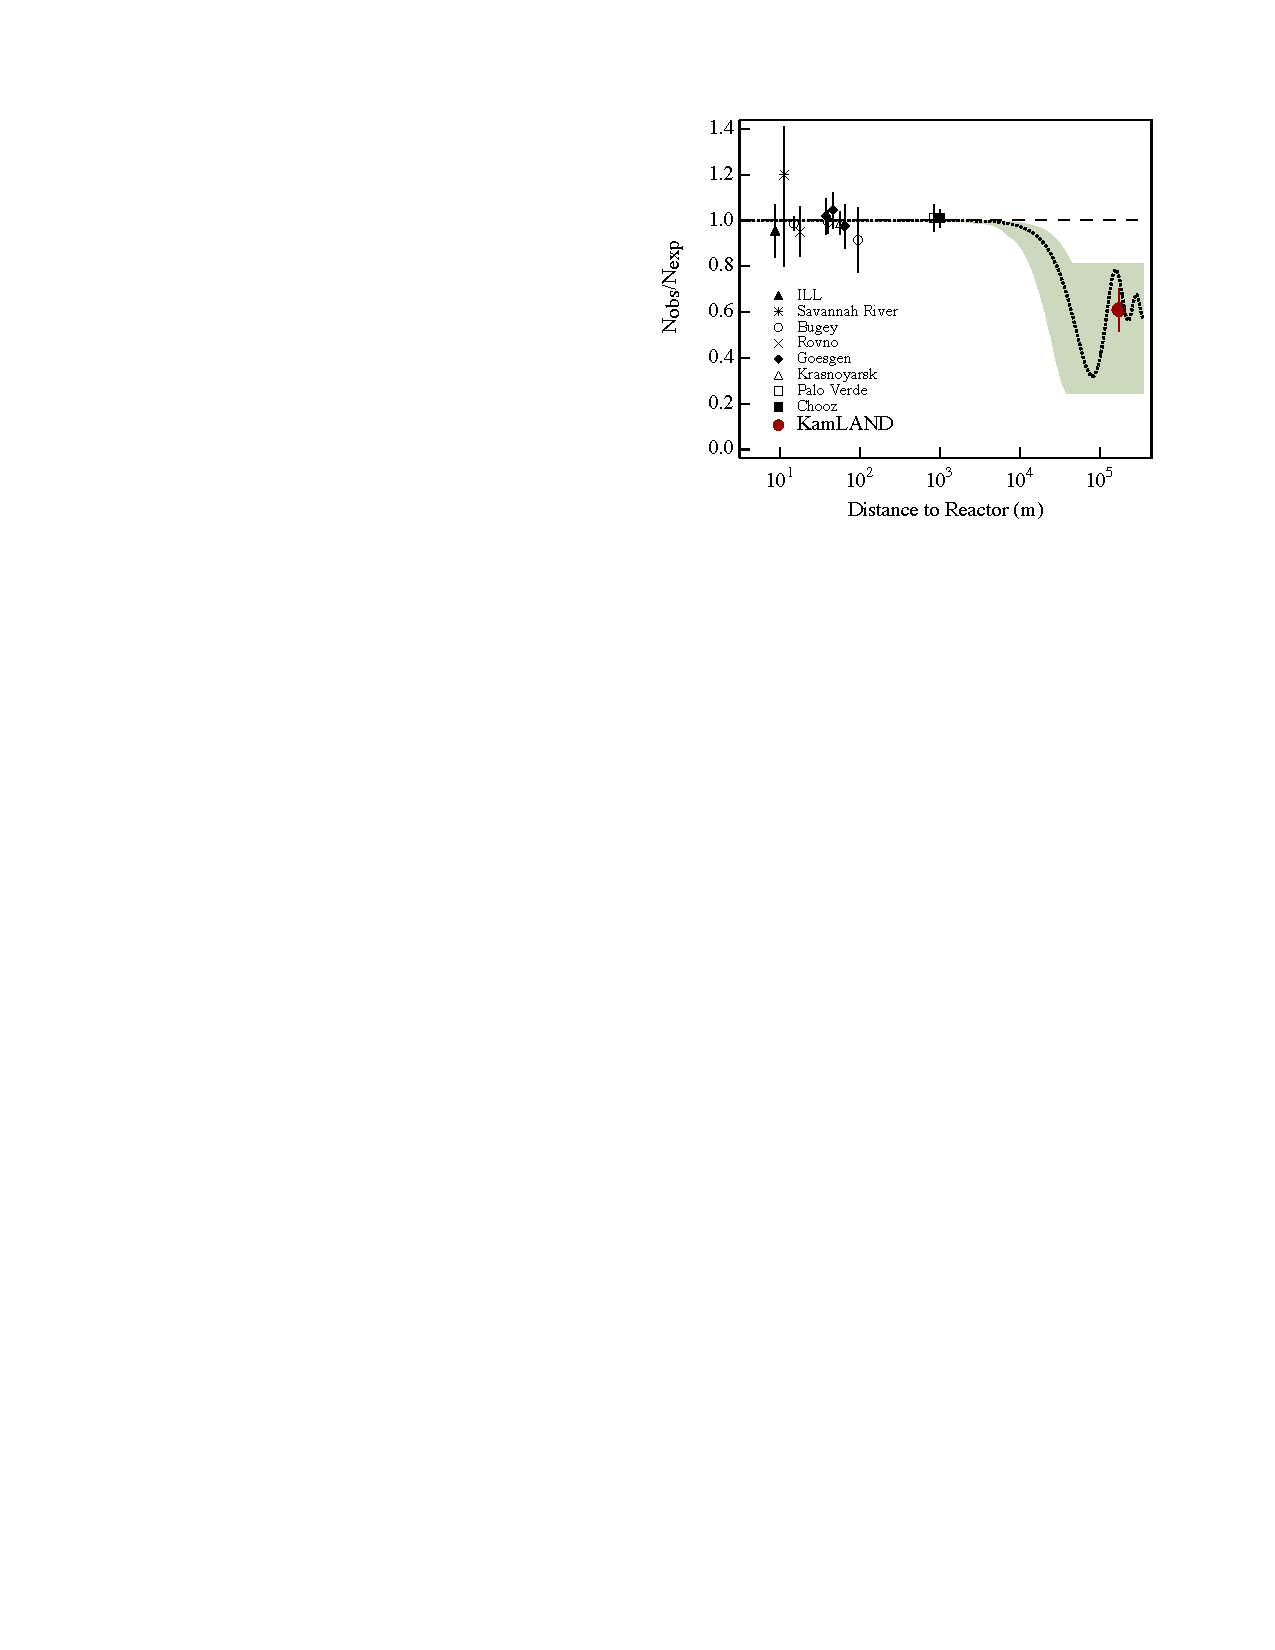
\includegraphics[width=60mm]{Figures/KamLANDFlux.pdf}}
    \subfigure[]{\label{fig:kamLE}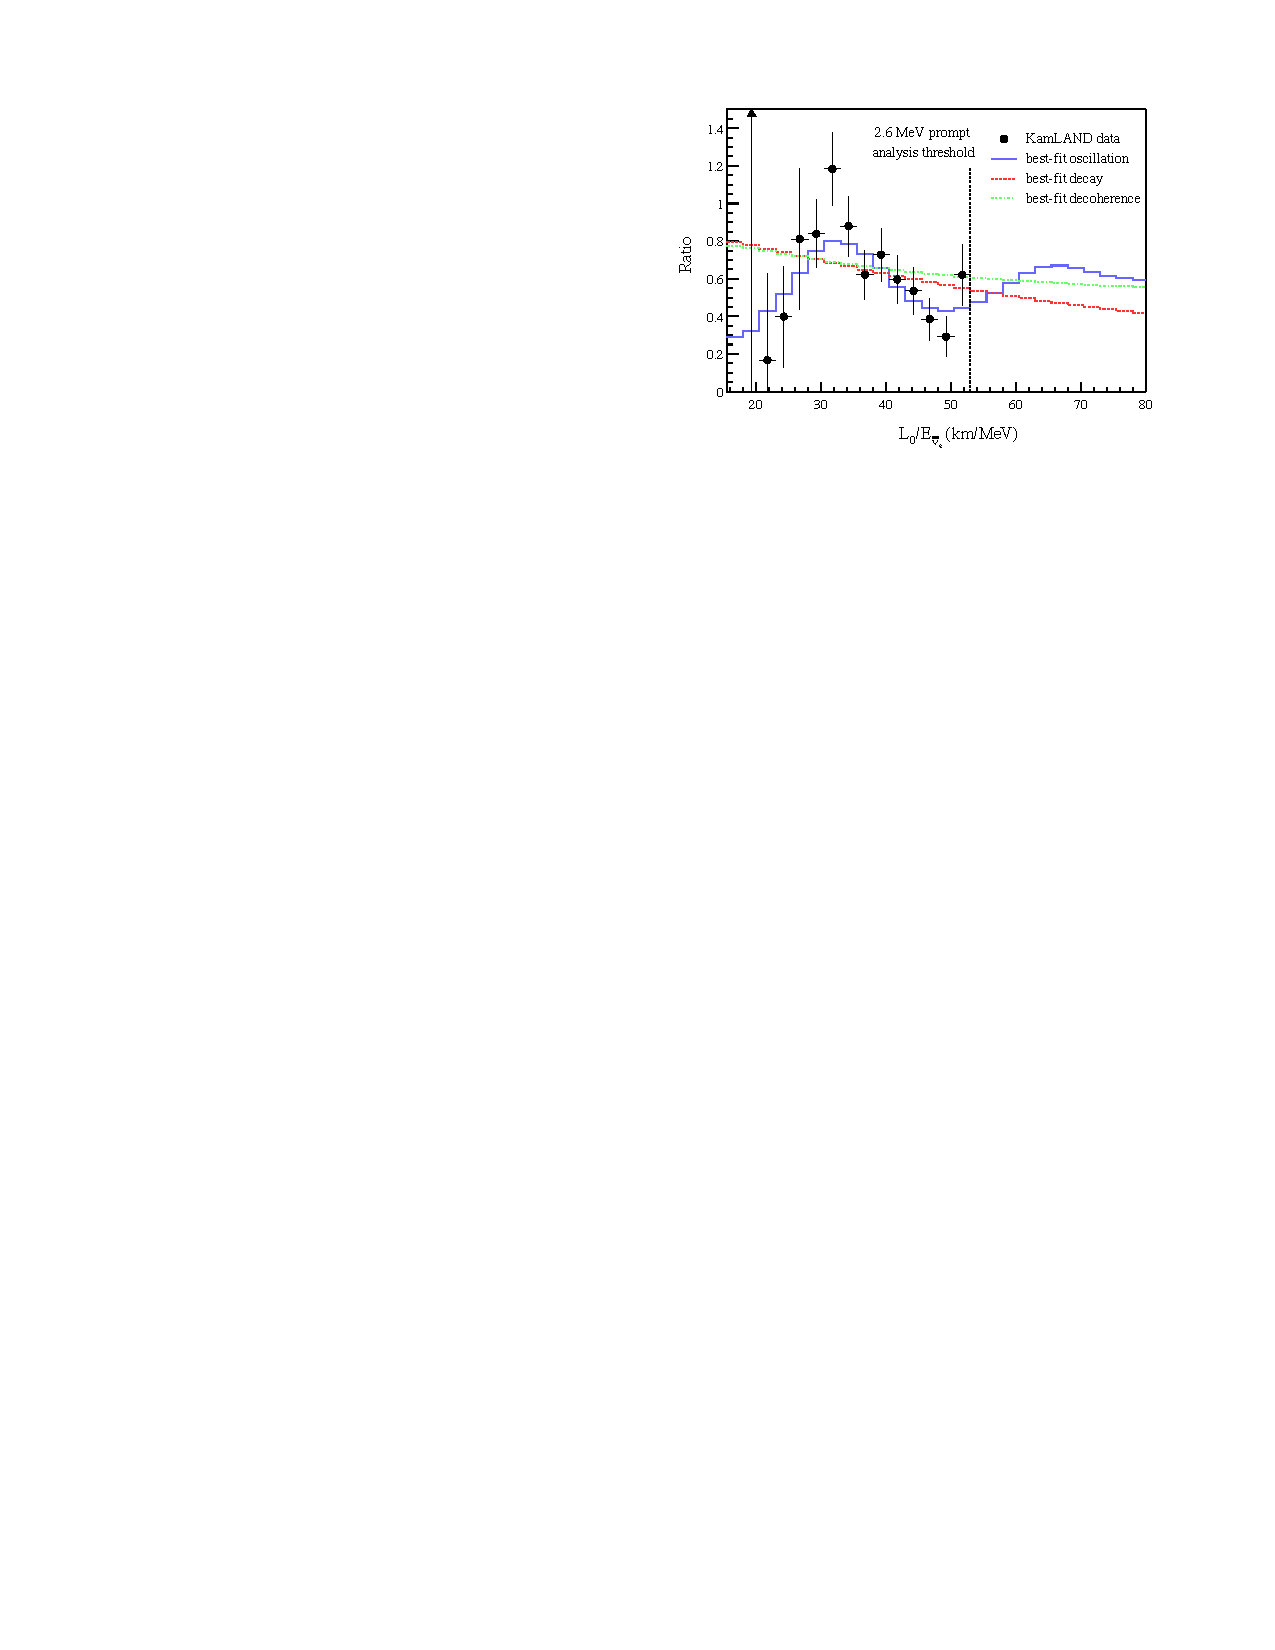
\includegraphics[width=60mm]{Figures/KamLANDLE.pdf}}
    \caption[Confirmation of Reactor Neutrino Oscillation by KamLAND]{The observation of reactor neutrino oscillation by KamLAND.
    (a) The ratio of the KamLAND observed neutrino flux to ILL+Vogel prediction.
    (b) The ratio of KamLAND measured $L_0/E$ spectrum to no oscillation prediction with average baseline $L_0 = 180$~km, indicating oscillation behavior with respect to $L_0/E$ of \nuebar.
    This result also disfavored neutron decay and decoherence model made based on atmosphere neutrino experiment.}
    \label{fig:Kamland}
    \end{figure}
    
    Another milestone in the reactor neutrino experiments is the precise measurement of the $\theta_{13}$ mixing angle. 
    Historically, the medium baseline experiments, CHOOZ~\cite{bib:chooz03}, Parlo Verde~\cite{bib:palo2000}, RENO~\cite{bib:RENO}, Daya Bay~\cite{bib:DYBosc} and Double CHOOZ~\cite{bib:DBChooz} experiments attempted to measure $\theta_{13}$ by observing the $\nuebar\rightarrow\nuebar$ disappearance in baselines varying from several hundred meter to 1~km from commercial reactors.
    Following CHOOZ and Parlo Verde's measurement of the $\sin^22\theta_{13}$ upper bound, RENO, Daya Bay and Double CHOOZ independently reported the measurement of non-zero $\theta_{13}$ mixing angle.
    The three $\theta_{13}$ experiments all utilized Gd loaded LS detectors deployed at different baselines from groups reactors.
    By comparing the \nuebar flux between near and far detectors, these experiments measured the $\nuebar\rightarrow\nuebar$ disappearance probability independently from nuclear model of the reactors.
    The result of the measurements is shown in Table~\ref{tab:1.1}.
    \begin{table}[h]
    \centering
    \begin{tabular}{lllll}
    \hline
    Experiment  & Baseline   & Average Fission Fraction   \\ 
    \hline
    Daya Bay     & 560~m to 1640~m  & 5.71\% $^{235}$U, 29.9\% $^{239}$Pu, 7.6\% $^{238}$U, 5.4\% $^{241}$Pu \\
    \hline
    RENO     & 294~m to 1383~m & 5.73\% $^{235}$U, 29.9\% $^{239}$Pu, 7.3\% $^{238}$U, 5.5\% $^{241}$Pu \\
    \hline
    Double CHOOZ    & 1050~m & 48.8\% $^{235}$U, 35.9\% $^{239}$Pu, 8.7\% $^{238}$U, 6.7\% $^{241}$Pu \\
    \hline
    \hline
    \end{tabular}
    \caption[$\theta_{13}$ reactor experiments]{The medium baseline reactor neutrino experiments that measured $\theta_{13}$ mixing angle.
    The commercial reactors utilized in these experiments are contains various effective fission fractions that evolve with time.}
    \label{tab:theta13}
    \end{table}

\Section{Reactor Antineutrino Anomaly}
\label{c2s3}
        
    In addition to the oscillation measurement, the $\theta_{13}$ experiments also measured absolute neutrino flux and spectrum of commercial reactors. 
    To provide precise models for these measurements, predictions of reactor neutrino flux and spectrum is revisited with both the \textit{ab initio} method and the $\beta$ conversion method.
    
    The Mueller model~\cite{bib:mueller} read the ENSDF and JENDL nuclear databases to sum the \nuebar spectrum from the $\beta$ branches.
    This method also used the branching fraction of from the databases to fit the ILL measurement in 1980s and calculated the \nuebar spectra of $^{235}$U, $^{238}$U, $^{239}$Pu, and $^{241}$Pu.
    The Huber model~\cite{bib:huber} utilized the $\beta$ spectra of $^{235}$U, $^{239}$Pu, and $^{241}$Pu measured from the ILL reactor and applied the conversion method with higher order theoretical corrections to the $\beta$ spectra of the virtual decay branches.
    The theoretical corrections include the effect of electron-nucleus interaction, photon radiation, and weak magnetism correction. 
    With different approaches of theoretical distribution, Mueller model of expected neutrino flux found 2.5\% more than the ILL+Vogel model, and Huber model found 3\% increase in neutrino flux prediction.
    However, the absolute flux measurements of the historical reactor experiments within 1~km baseline showed inconsistent reactor neutrino flux with either of the prediction, as shown in Figure~\ref{fig:DYBFlux}.
    \begin{figure}[h!]
    \centering
    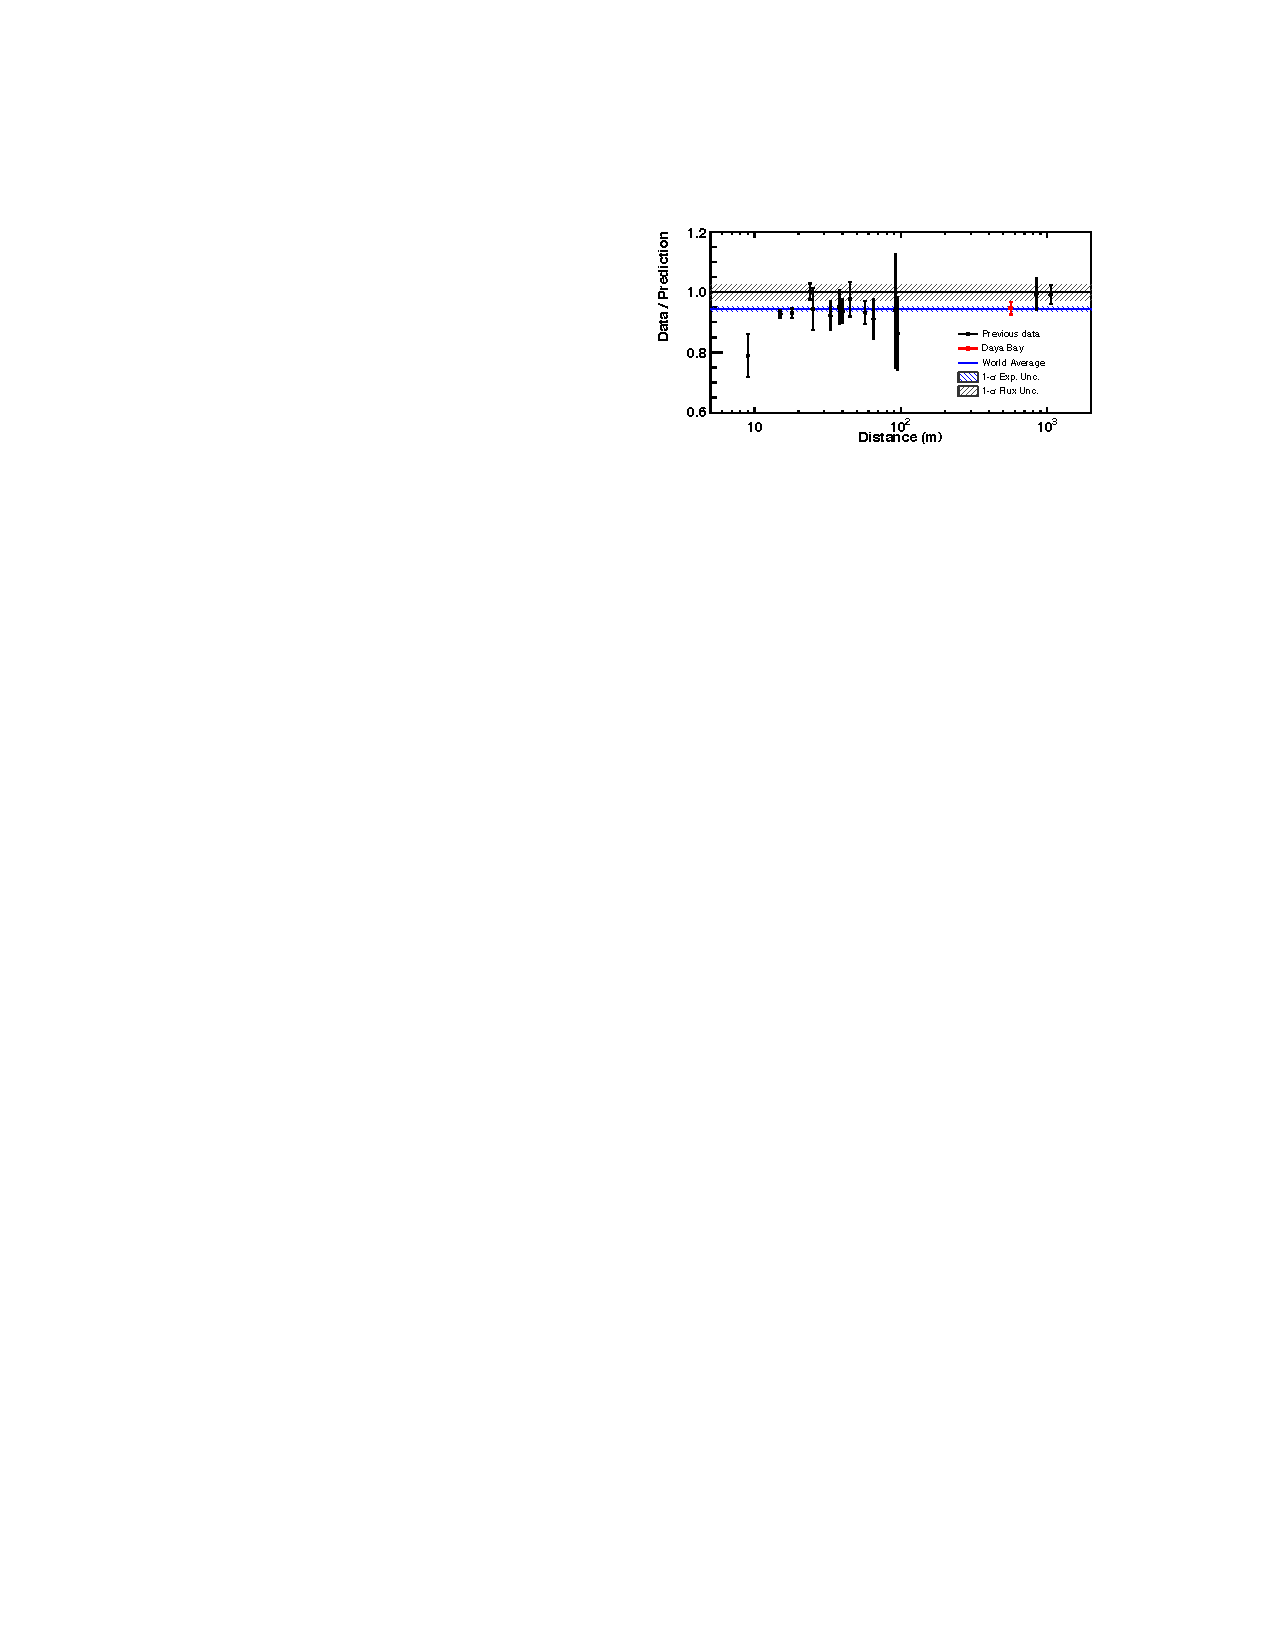
\includegraphics[width=0.6\textwidth]{Figures/DYBGlobalFlux.pdf}
    \caption[Daya Bay Absolute Reactor Neutrino Flux]{Historical reactor neutrino flux measurements \cite{bib:DYB2015}.
    The global average is 5\% to 6\% deficit from Huber+Mueller predicted flux.}
    \label{fig:DYBFlux}
    \end{figure}
    
    The neutrino flux deviation is referred as the Reactor Antineutrino Anomaly (RAA)~\cite{bib:RAA}.
    This anomaly suggests a systematic bias present in the theoretical aggregation method and/or the virtual branching approach in the conversion from the ILL measured $\beta$ spectrum.
    This disagreement of neutrino flux in the medium baselines can also be explained by a possible oscillation between \nuebar and a light sterile neutrino.
    A 3+1 model of left hand neutrino mixing with sterile neutrino with $\Delta m^2$ in $\sim$1~eV$^2$ scale is developed based on the disappearance rate shown in the flux deficit.
    The RAA best fit 3+1 neutrino oscillation parameters are shown in Fig.~\ref{fig:RAA}.
\begin{figure}[h!]
    \centering
    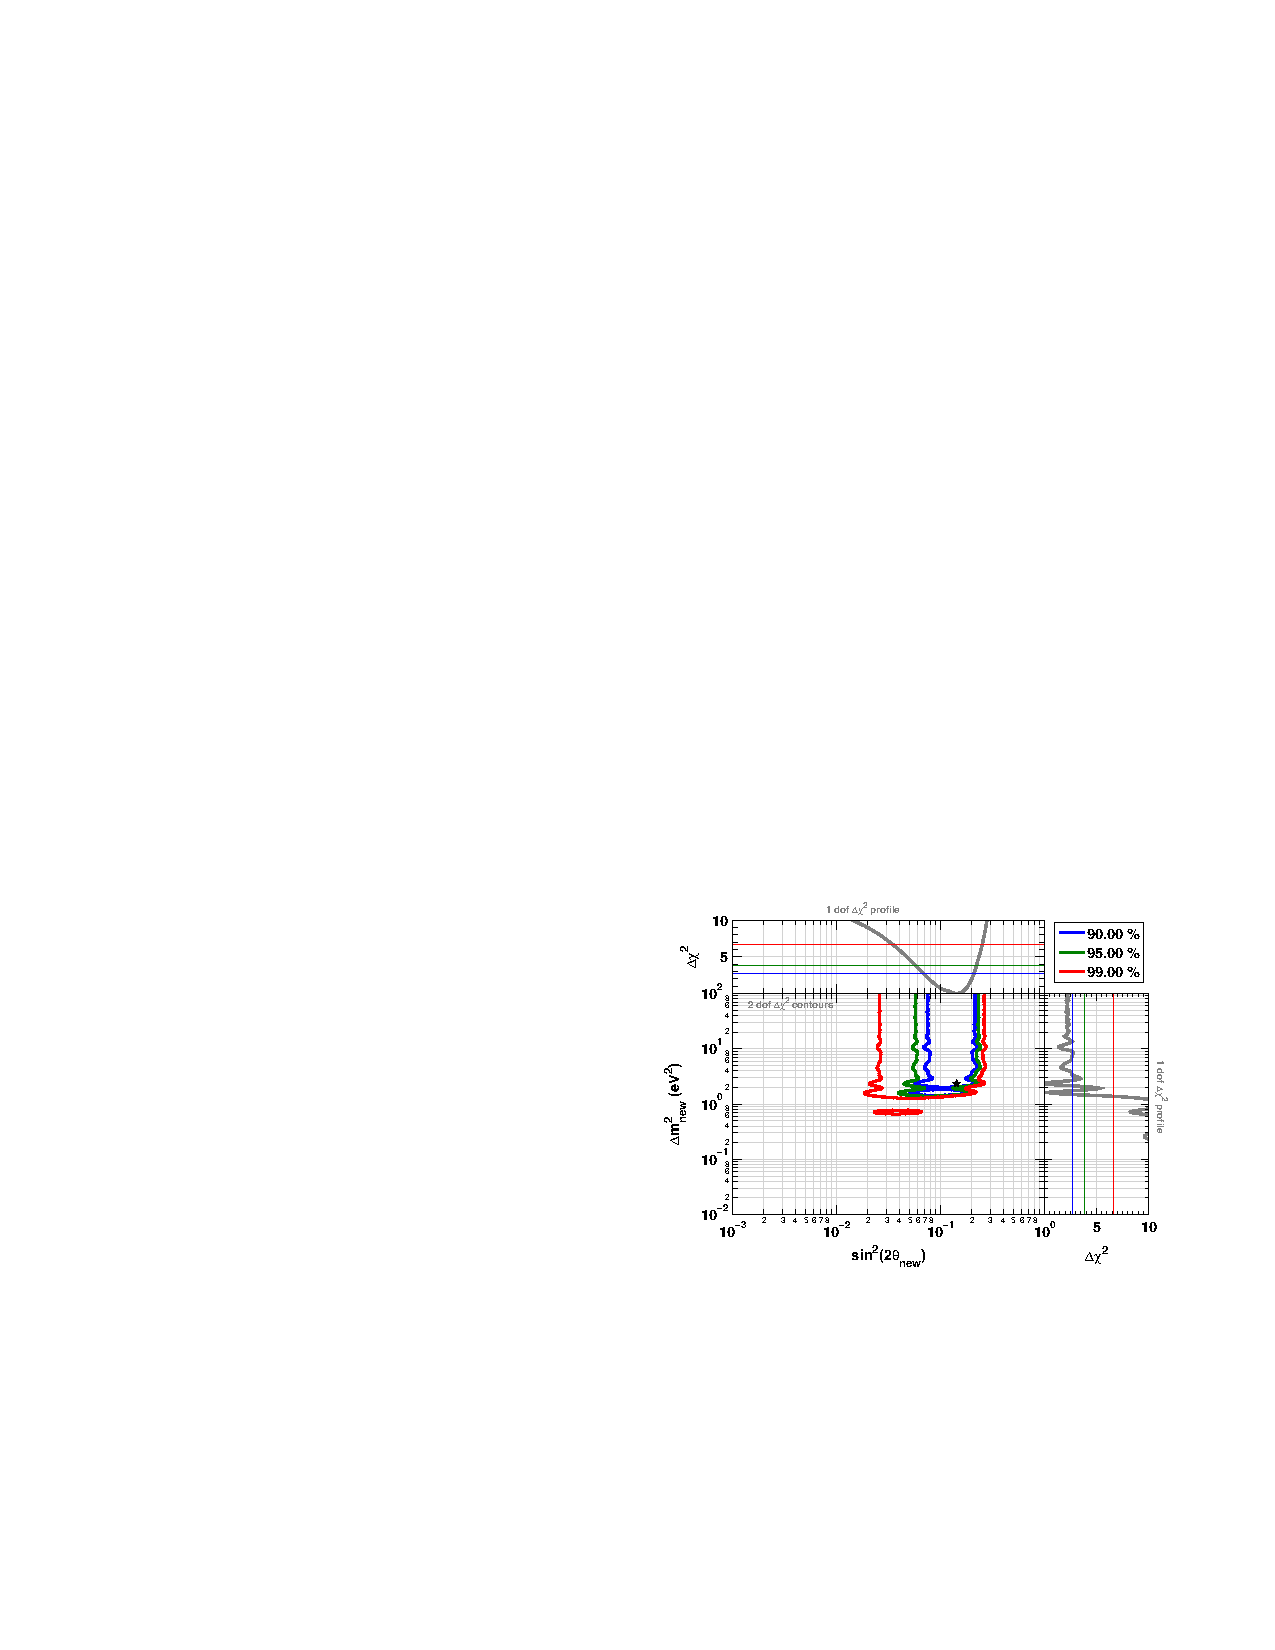
\includegraphics[width=0.6\textwidth]{Figures/RAA3plus1.pdf}
    \caption[The allowed region for the parameters of sterile oscillation]{The allowed region for the parameters of the sterile neutrino oscillation as a result of the flux deficit observed in RAA~\cite{bib:RAA}. The best fit point suggests a $\sin_{14}^22\theta = 0.14\pm0.08$ and $|\Delta m^2| > 1.5$~eV$^2$ (95\% C.L.) of a 3+1 left hand neutrino and sterile neutrino mixing.}
    \label{fig:RAA}
\end{figure}

    In dependent of the flux deviation, the medium baseline experiments, Daya Bay~\cite{bib:DYBSpectrum}, Double CHOOZ~\cite{bib:DBChooz} and RENO~\cite{bib:RENO}, also measured reactor neutrino spectrum disagreeing to the Huber and Mueller models, as shown in Fig.~\ref{fig:DYBSpectrum}.
    An 8\% to 10\% excess is observed in the 4~MeV to 6~MeV region of IBD positron energy, equivalent to 5~MeV to 7~MeV reactor neutrino energy.
    With high statistical significance, the spectral deficit also hints errors in the nuclear database used to calculate the expected spectral shape.
    Additionally, the isotopic contribution to the flux and spectrum anomaly is unclear due to the mixture and evolution of the fission isotopes in Low Enrichment Uranium (LEU) reactors utilized by these experiments.
 \begin{figure}[h!]
    \centering
    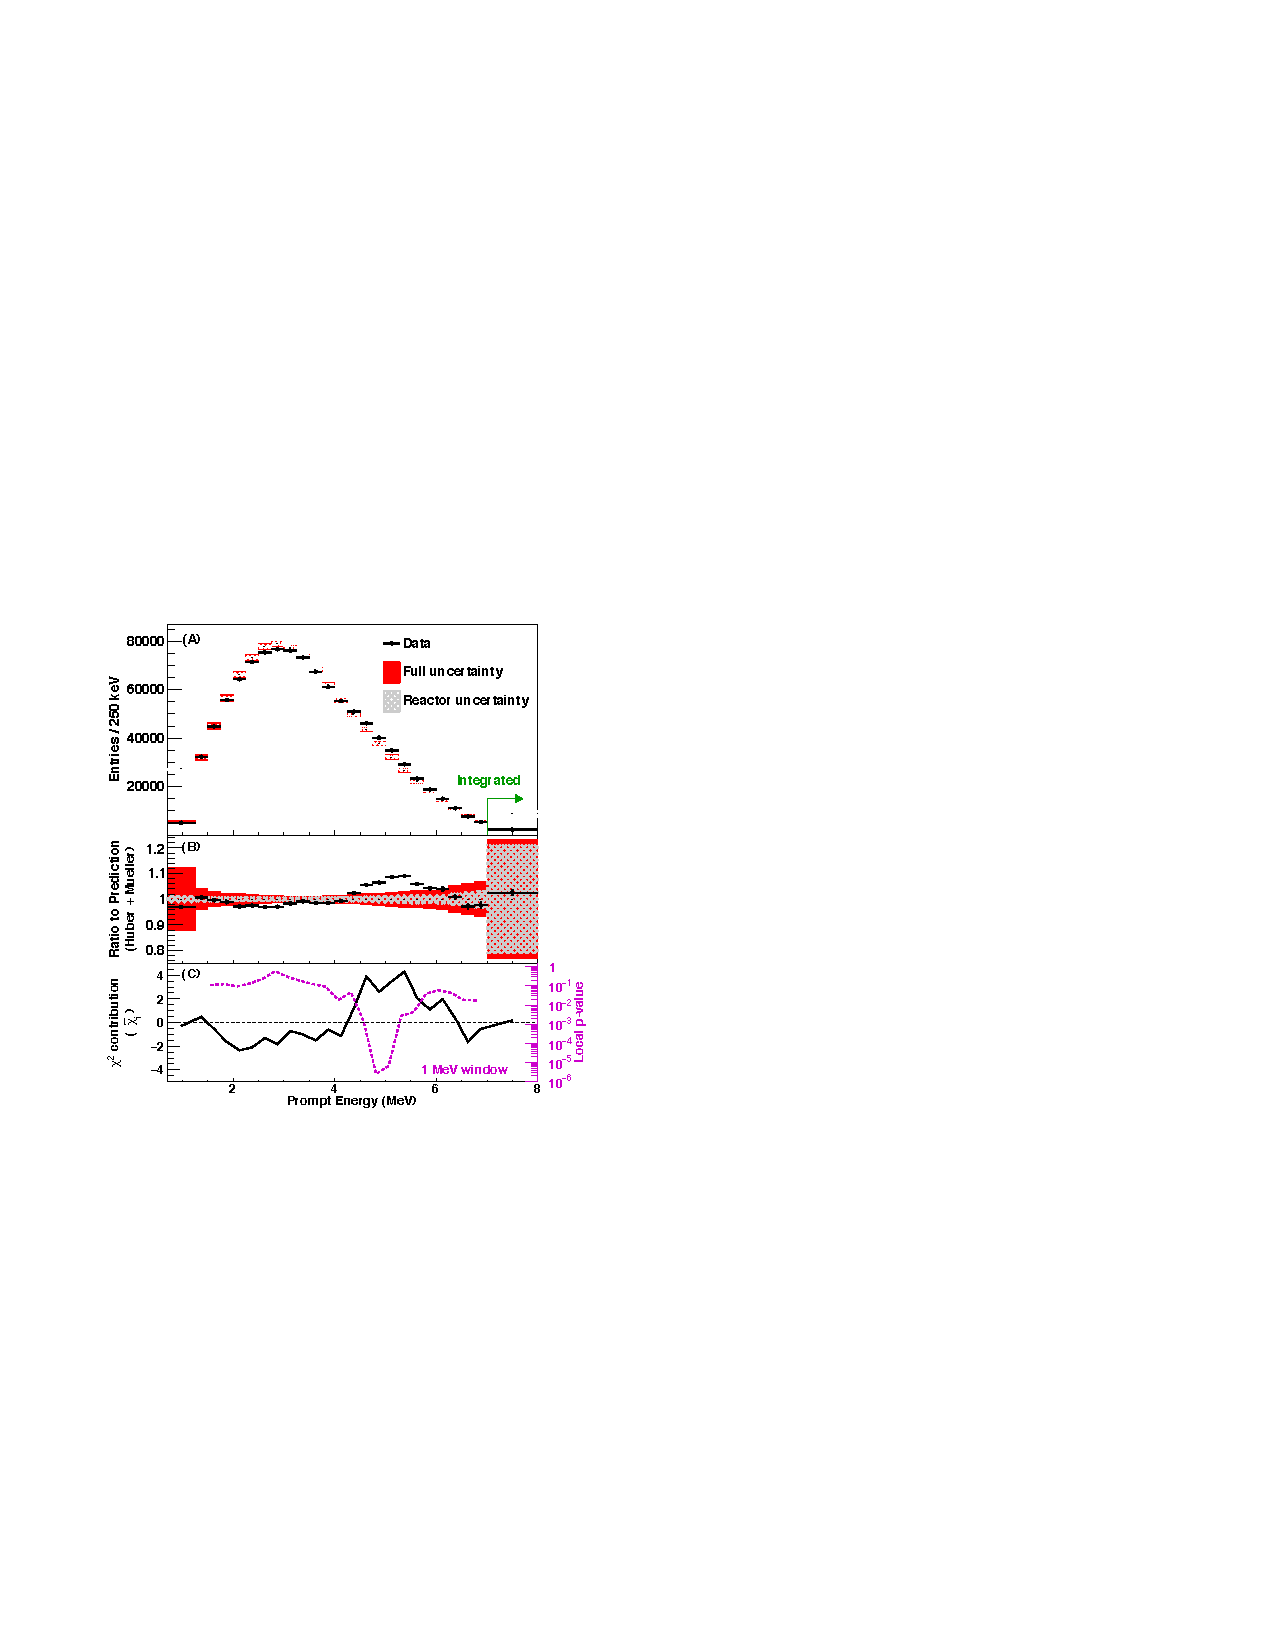
\includegraphics[width=0.6\textwidth]{Figures/DYBSpectrum.pdf}
    \caption[Daya Bay IBD positron energy spectrum]{The IBD positron energy spectrum measured by Daya Bay experiment.
    The spectrum is the sum of IBD positron spectrum from four fission isotopes, which indicate an excess at 4~MeV to 6~MeV compared to the Huber+Mueller model with 2.9~$\sigma$ discrepancy.}
    \label{fig:DYBSpectrum}
    
\end{figure} 
    
\Section{Resolution to the RAA}

    Further studies, including introducing forbidden transition in fission branches~\cite{bib:hayes} and \textit{ab initio} spectrum prediction with different nuclear databases~\cite{bib:dywer}.
    These studies suggested larger systematic uncertainty of branching in Huber+Mueller model because of the lack of forbidden branching knowledge and errors in nuclear databases.
    Phenomenological studies~\cite{bib:giunti2019} based on historical reactor experiments were also made to resolve the RAA by comparing neutrino flux of reactors with various fission fractions.
    The global fit of isotopic contribution to the flux deficit hints $^{235}$U to be the main contributor. 
    
    Multiple reactor neutrino measurement have been made in resolving the isotopic contribution of the flux and spectrum anomaly.
    Daya Bay and RENO experiments measured the reactor neutrino flux and spectrum evolution dependent on nuclear fuel fraction~\cite{bib:DYBEvo, bib:RENOevolution}. 
    These measurements indirectly tested the contribution of $^{235}$U and $^{239}$Pu's contribution to the reactor neutrino flux and spectrum deficit.
    In the fuel evolution measurements, the reactor neutrino flux and spectrum's dependence to fission isotopes is observed.
    The evolution of spectrum also weakly hinted the correlation between $^{235}$U-$^{239}$Pu transition and the local excess of the IBD spectrum.

    The lack of definitive resolution to the RAA brought the necessity of a direct measurement of the reactor neutrino flux and spectrum from a single fission isotope, typically $^{235}$U.
    A very short baseline, $^{235}$U only reactor neutrino experiment is preferred to measure the flux and spectrum of \nuebar to probe the 1~eV scale sterile neutrino oscillation and the isotopic contributions to the RAA.

\Chapter{PROSPECT Experiment}
    
    The RAA described in Chapter~\ref{Ch2} leads to the need of an experiment able to probe the short baseline sterile neutrino oscillation, as well as direct measurement of the flux and spectrum of a single fission fuel reactor. 
    The experiment has to meet the requirements of 
    \begin{itemize}
        \item Sub-10~m baseline from a reactor with compact reactor size. 
        \item Fission reactor whose neutrino production is from a single isotope.
        \item High IBD position reconstruction for oscillation measurement.
        \item High energy resolution to precisely measure neutrino spectrum.
    \end{itemize}
    
    PROSPECT~\cite{bib:prospect_physics, bib:prospect_nim}, the Precision Reactor Oscillation and SPECTrum experiment, was designed and built to direct measure neutrino fluxa and spectrum from the High Flux Isotope Reactor (HFIR) located at Oak Ridge National Laboratory (ORNL), USA. 
    PROSPECT's antineutrino detector (AD) covers various baseline from 7~m to 9~m with segmented LS.
    The goal of PROSPECT is to probe the $\sim$1~eV scale sterile neutrino oscillation by the observation of \nuebar disappearance, and precisely measure reactor neutrino spectrum from only $^{235}$U.
    
\Section{HFIR Reactor}

    HFIR reactor is a high enrichment $^{235}$U (HEU) research fission reactor, whose $^{235}$U enrichment is 93\% in average.
    The key parameters of HFIR reactor for PROSPECT neutrino measurement are shown in Table~\ref{tab:HFIR}.
\begin{table}[h]
    \centering
    \caption[HFIR parameters]{The properties of the HFIR reactor.}
    \begin{tabular}{cc}
    \hline
    \hline
    Parameter  & Value   \\
    \hline
    Power    & 85~MW \\
    Dimensions     & 435~mm (diameter) $\times$ 508~mm (height) \\
    $^{235}$U enrichment & 93\% \\
    Neutrino source & $\sim$99\% from $^{235}$U \\
    Reactor cycle & $\sim$25~day on, $\sim$30~day off \\
    \hline
    \end{tabular}

\label{tab:HFIR}
\end{table}

\begin{figure}
    \centering
    \includegraphics[width=0.5\textwidth]{Figures/HFIR.pdf}
    \caption[The dimensions and power distribution of HFIR]{A model of the reactor~\cite{bib:prospect_nim} parameters (a) and (b) are the diameter and height of the HFIR core.
    The location of the HFIR core in a detailed reactor system simulation is indicated in (c).
    (d) is a projection of the fission power density of HFIR at the x-z plane.}
    \label{fig:HFIR}
\end{figure}

    HFIR is a cylindrical fission reactor.
    Its compact size, as shown in Table~\ref{tab:HFIR} and Figure~\ref{fig:HFIR}, is ideal to limit the uncertainty of baseline.
    To maintain its high $^{235}$U enrichment, the HFIR reactor has relatively short reactor cycles.
    In this case, the fuel evolution of fissile isotopes is negligible.
    
    The HFIR facility also brought unique challenge of background for neutrino measurement. 
    Because of the very short baseline requirement of the experiment and availability of the experiment site, the PROSPECT AD is exposed to cosmic ray background with minimal overburden. 
    The detector also faces reactor correlated background, e.g. the neutron background generated from reactor and the $\gamma$ ray background from the metallic materials in the piping of the facility.
    A comprehensive background characterization is therefore organized in the research and development (R\& D) phase of PROSPECT~\cite{bib:prospect_background}. 
    As a result, the amplitude of the gamma and neutron background is shown in Figure~\ref{fig:prospect_background}.
    The detector and additional background shielding was designed based on the by this background survey.
    
\begin{figure}
    \centering
    %\vspace{0pt}
    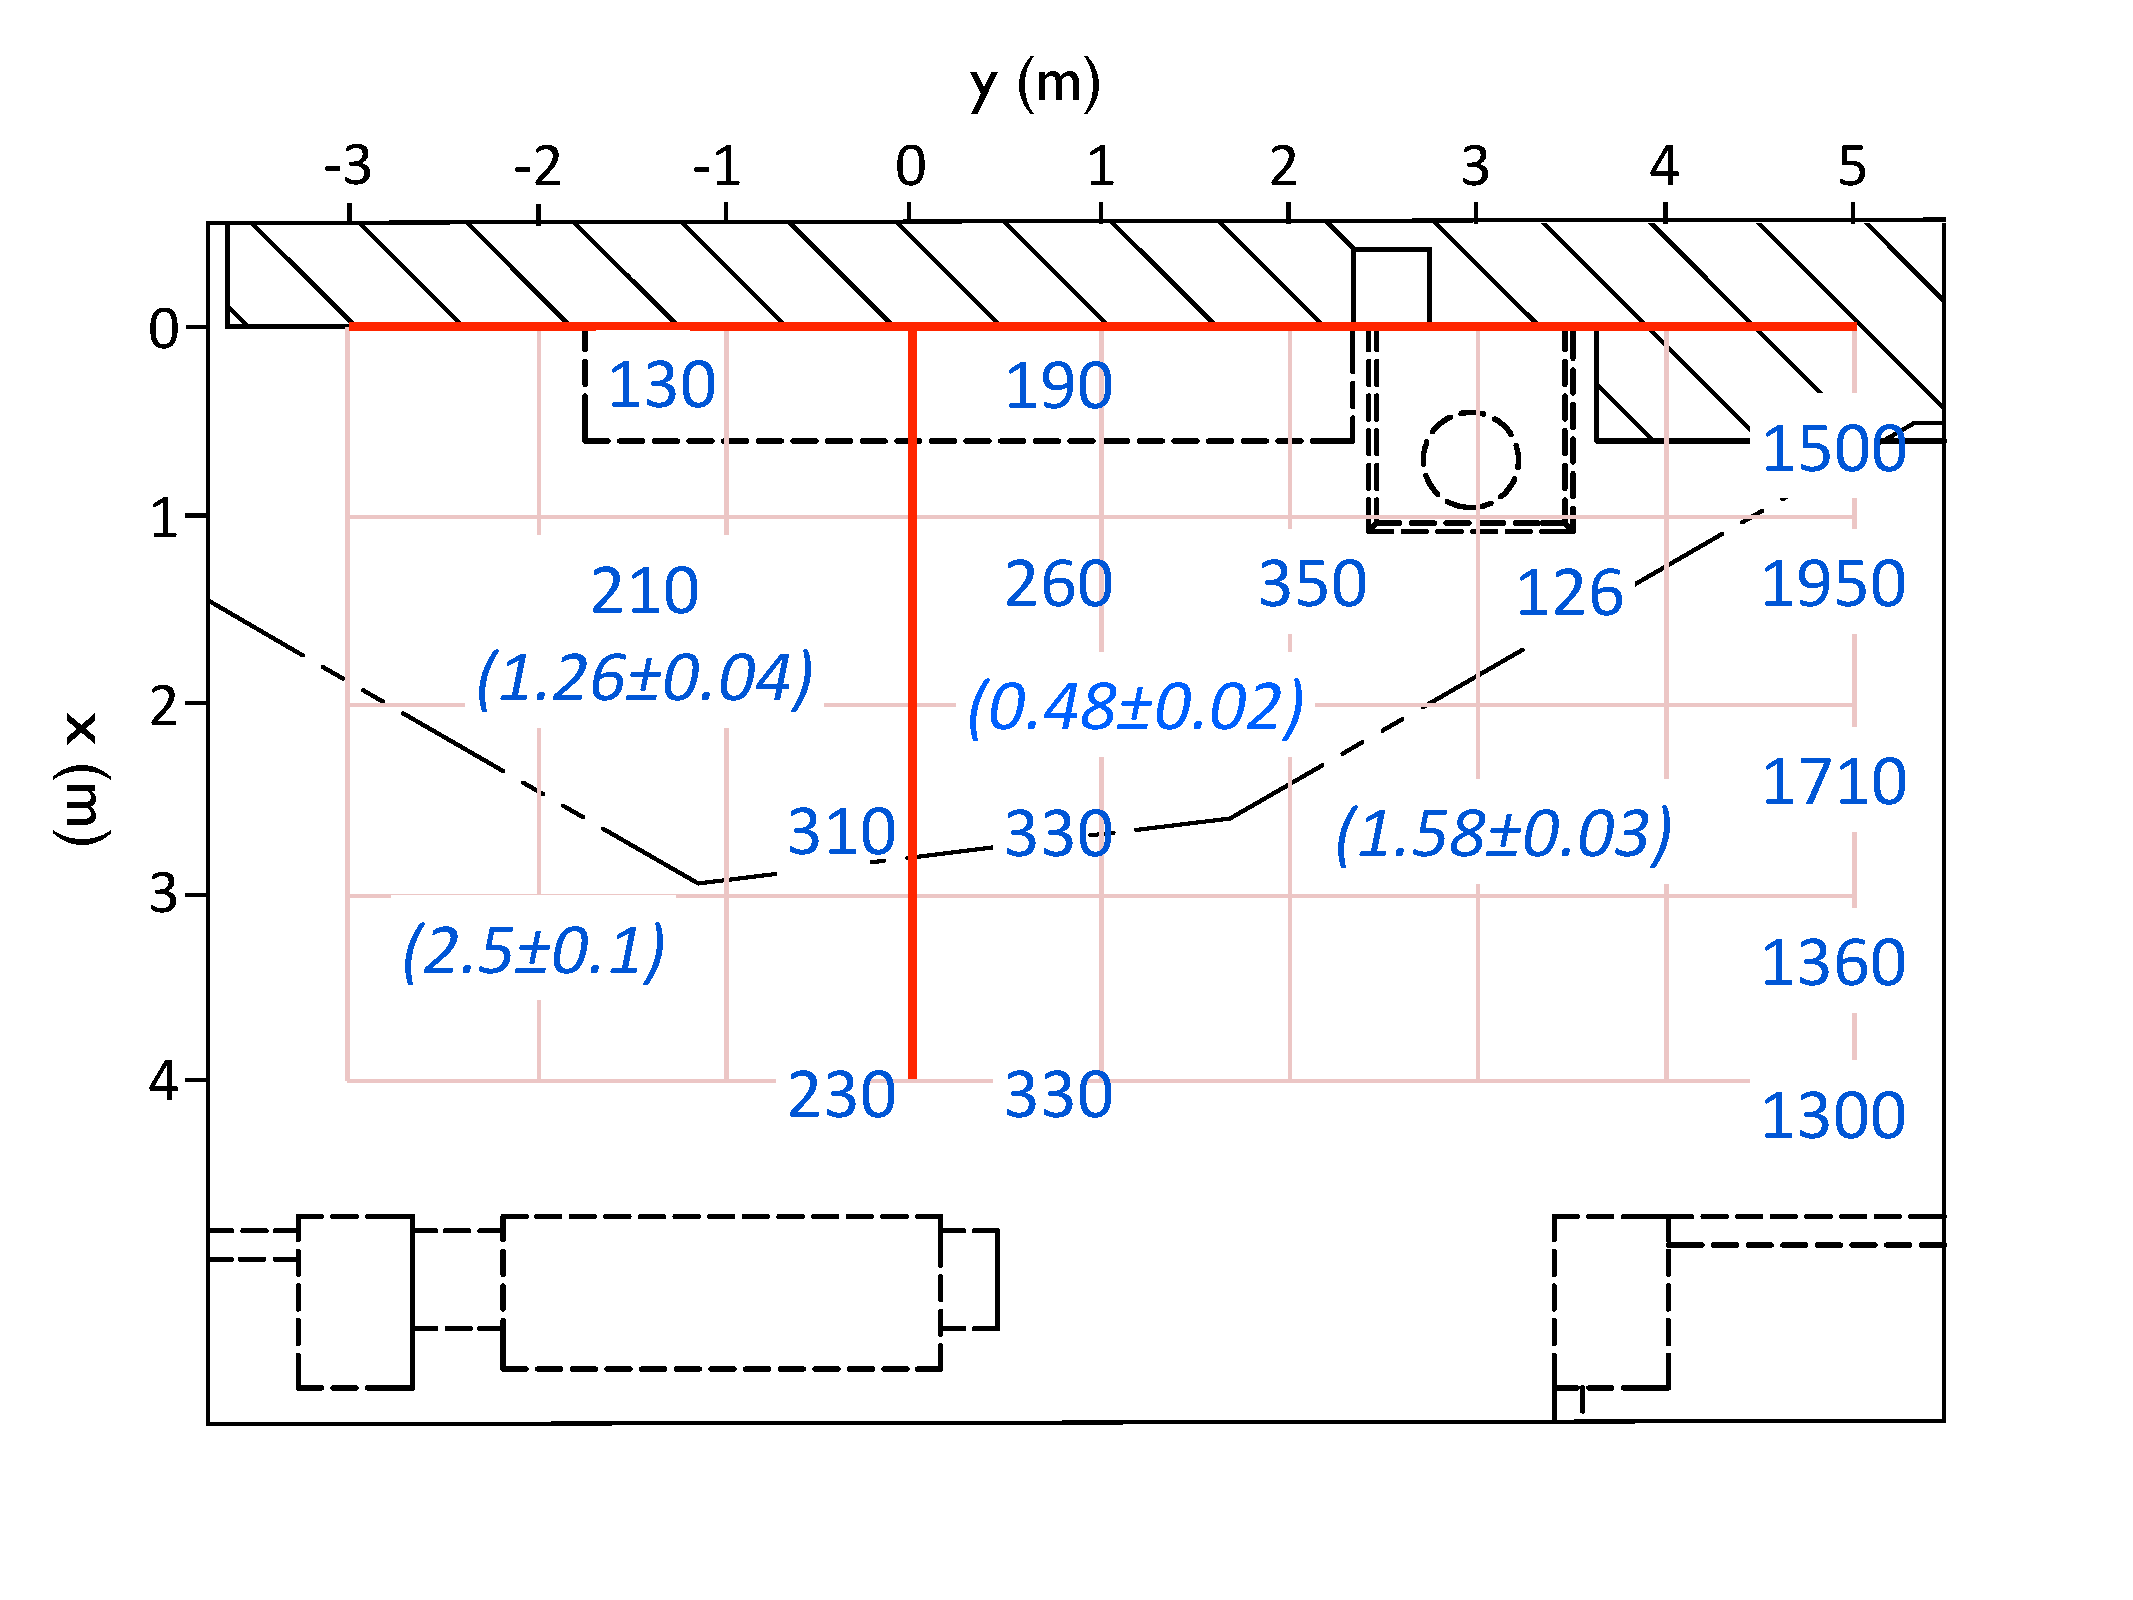
\includegraphics[width=0.47\textwidth, valign=t]{Figures/NeutronBGMap.pdf}
    %\vspace{0pt} 
    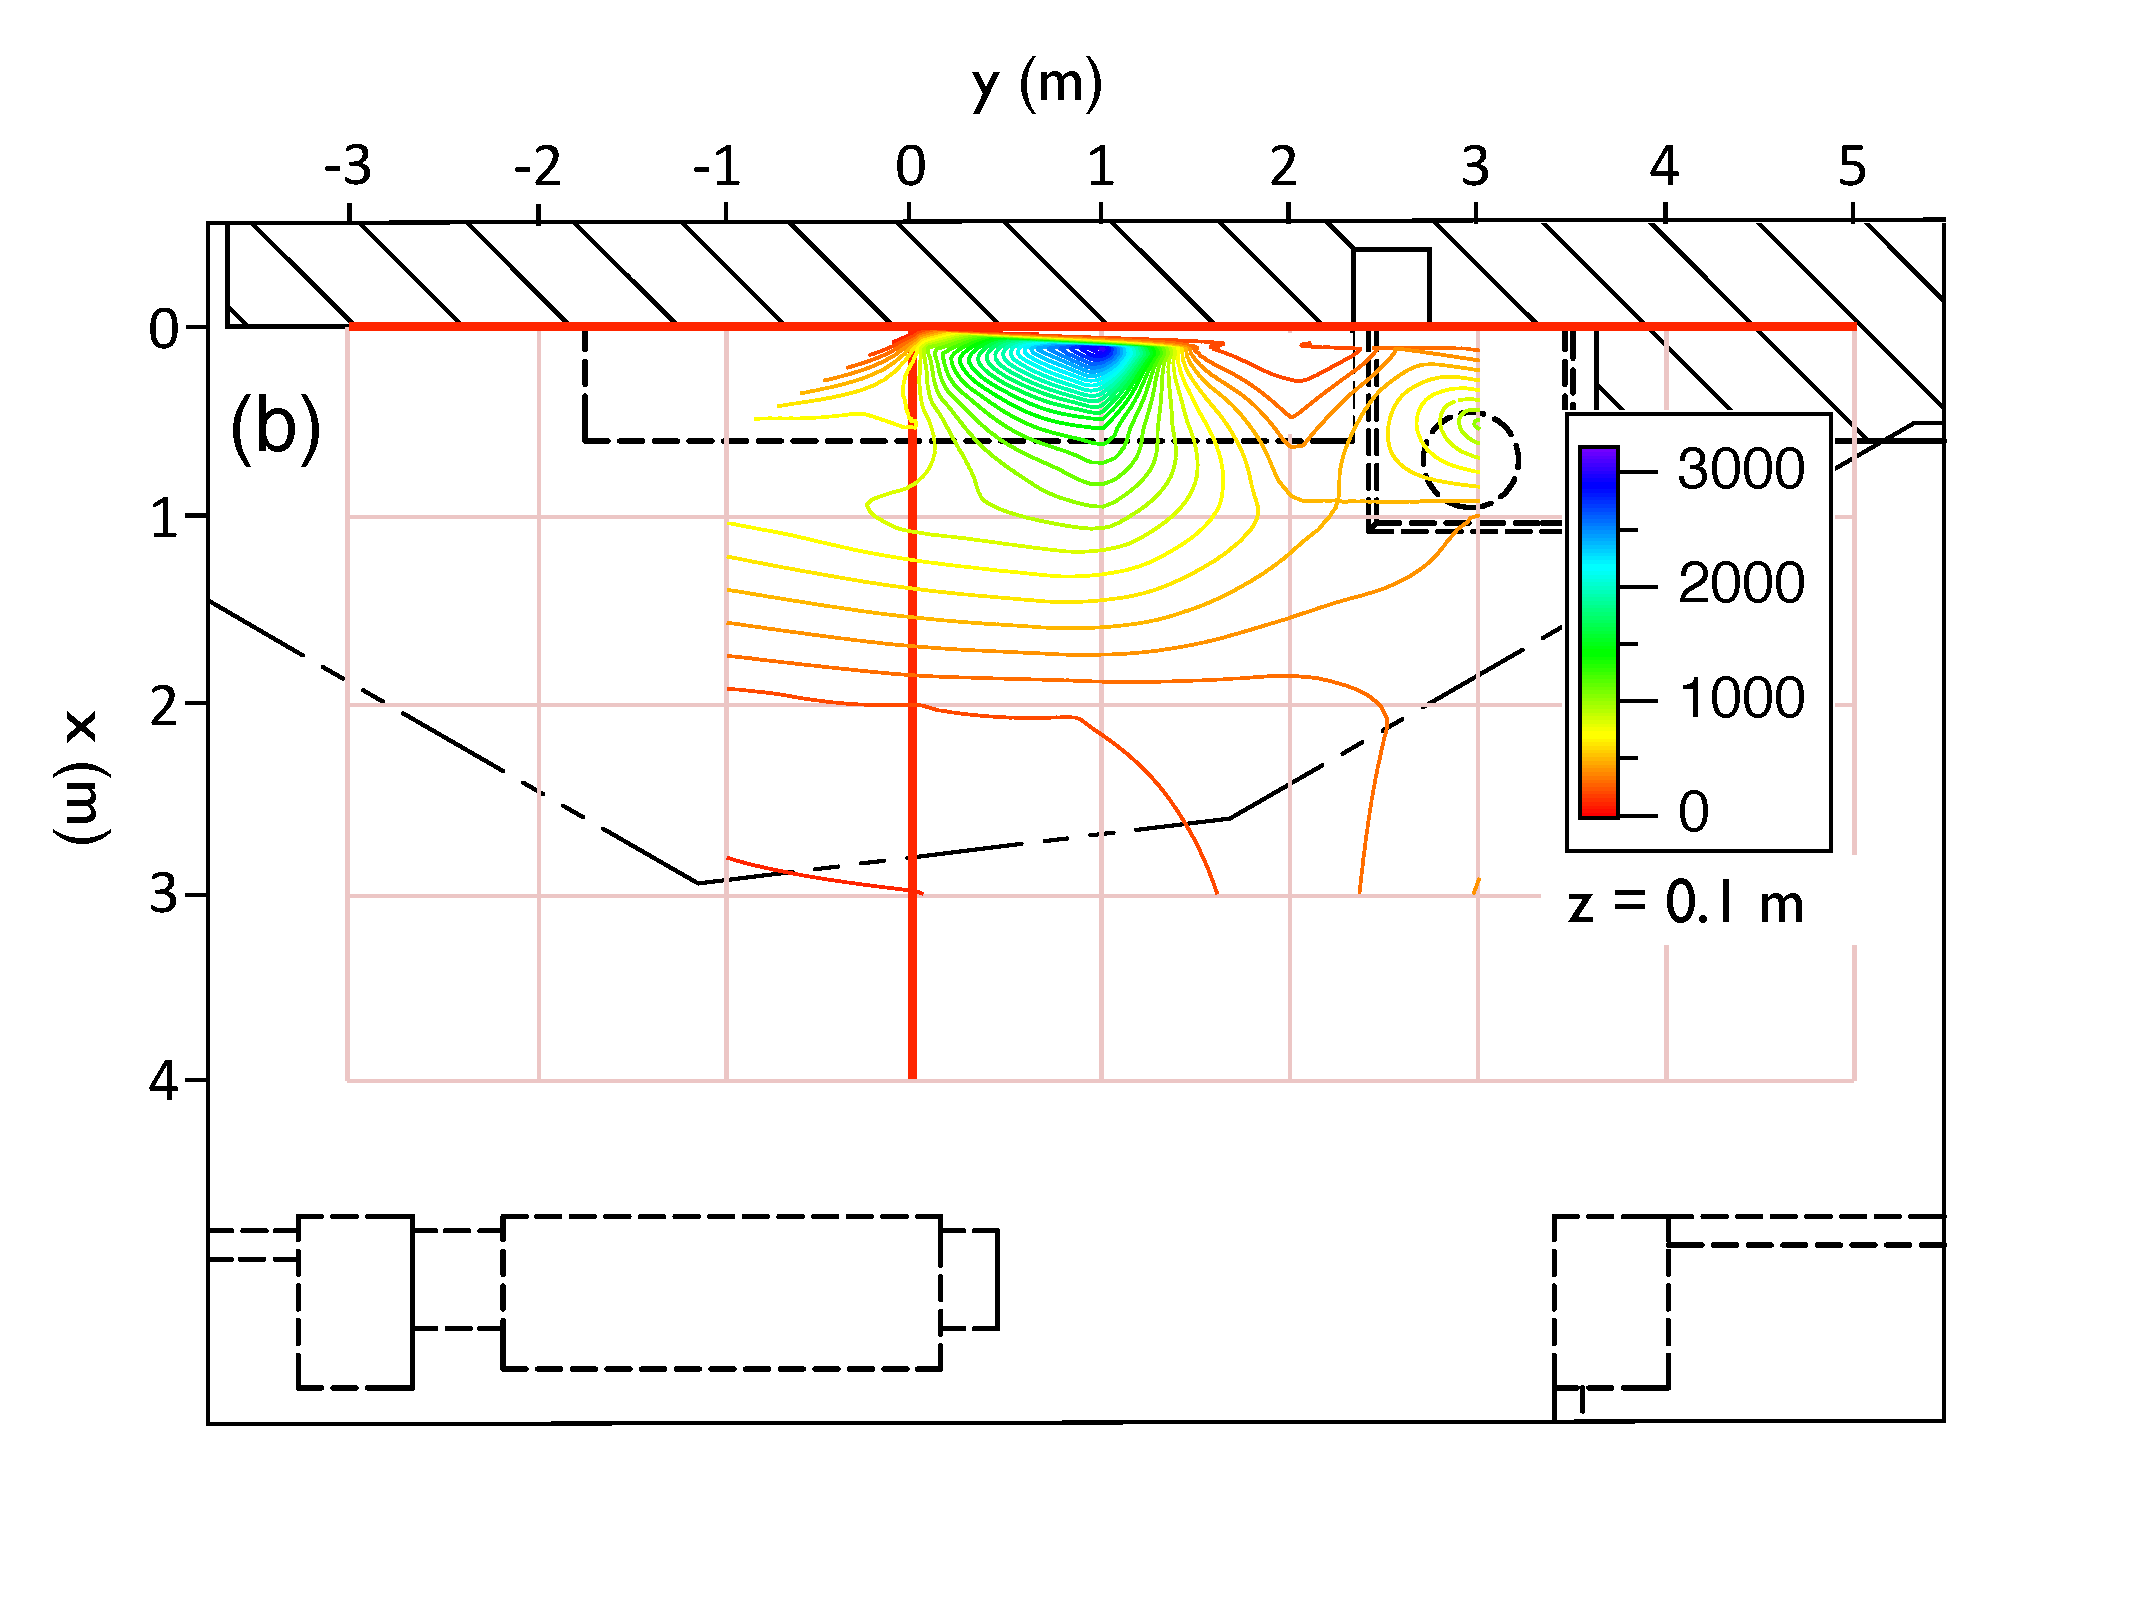
\includegraphics[width=0.51\textwidth, valign=t]{Figures/GammaBGMap.pdf}
    \caption[Local background distribution at HFIR facility]{(Left) The reactor correlated neutron background rate (nSv/h) shown in a map of the HFIR site where PROSPECT is deployed.
    (Right) The local $\gamma$ ray background rate (Hz) shwon in the same map.
    }
    \label{fig:prospect_background}
\end{figure}

\Section{Detector Design}

    The PROSPECT AD is a $\sim$4~ton $^{6}$Li-doped LS ($^{6}$LiLS) detector deployed at 7-9~m baselines from the HFIR core.
    The key parameters of the PROSPECT AD is shown in Table~\ref{tab:PROSPECT_AD}.
    The schematic of detector deployment at the HFIR facility is shown in Figure~\ref{fig:PROSPECT_LAYOUT}.
\begin{table}[h]
    \centering
    \caption[PROSPECT AD Parameters]{The key parameters of the PROSPECT AD~\cite{bib:prospect_nim}.}
    \begin{tabular}{cc}
    \hline
    \hline
    Parameter  & Value   \\ 
    \hline
    Target volume \& mass    & 3760 litters, 3.68 tons\\
    Target dimension & 1.176\,m wide $\times$ 2.045\,m long  $\times$ 1.607\,m tall \\
    Baseline     & 7.9~m \\
    Liquid scintillator & EJ-309 based LS with $<$0.1\% $^{6}$Li \\
    LS energy resolution & 4.5\% \\
    Segments & 14 horizontal $times$ 11 vertical \\
    Segment dimension & 1.176\,m wide $\times$ 14.5~cm long  $\times$ 14.5~cm tall \\
    Light collection & diameter = 12.7~cm (5~inch) PMTs\\
    Position resolution & $\sigma_X$ = 14.5~cm,  $\sigma_Y$ = 14.5~cm,  $\sigma_Z \approx$ 5~cm \\
    \hline
    \end{tabular}
    \label{tab:PROSPECT_AD}
\end{table}
\begin{figure}
    \centering
    %\vspace{0pt}
    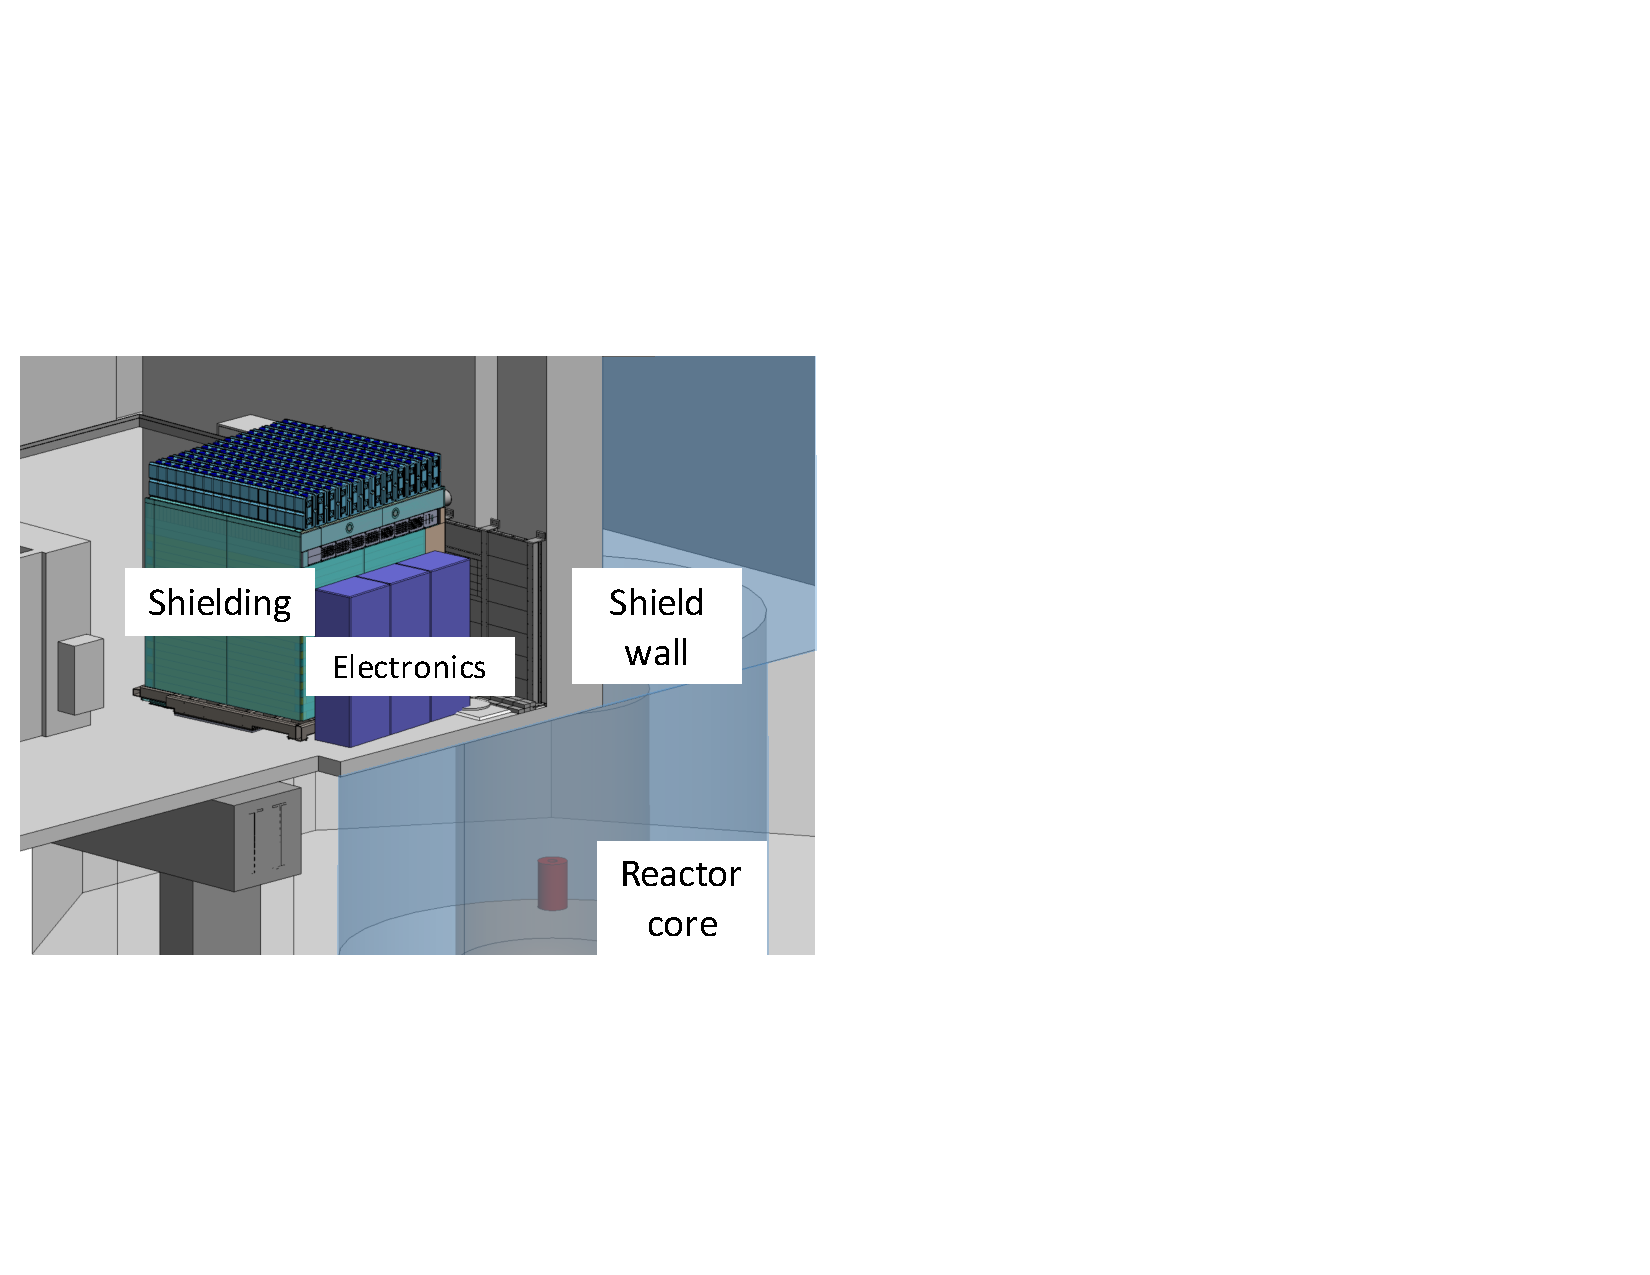
\includegraphics[width=0.6\textwidth]{Figures/Layout.pdf}
    \caption[The layout of the PROSPECT experiment]{The layout of the PROSPECT experiment.
    The PROSPECT AD is deployed 7.9~m from the reactor center to the detector center.
    Additional on site shield was installed between the reactor pool and the AD to eliminate the local $\gamma$ ray background.
    }
    \label{fig:PROSPECT_LAYOUT}
\end{figure}
    
    The anatomy of the PROSPECT AD is shown in Figure~\ref{fig:PROSPECT_AD}.
    The inner volume of the detector is contained in a liquid tight acrylic tank filled with the $^{6}$LiLS, which is made from the EJ-309 base, an organic LS \cite{bib:lspaper}.
    The acrylic tank shielded by layers of water, polyethylene, lead, borated polyethylene, respectively, from the exterior layer to interior to suppress neutron and gamma background.
    The designed energy resolution is 4.5\% to optimize PROSPECT's IBD spectrum measurement.
    An advantage of utilizing the EJ-309 is the pulse shape discrimination (PSD) feature making the PROSPECT AD sensitive to particle identity, which is described in detail in Section~\ref{sec:detection}.
    The $^{6}$Li is loaded as a main neutron capture isotope.

\begin{figure}
    \centering
    %\vspace{0pt}
    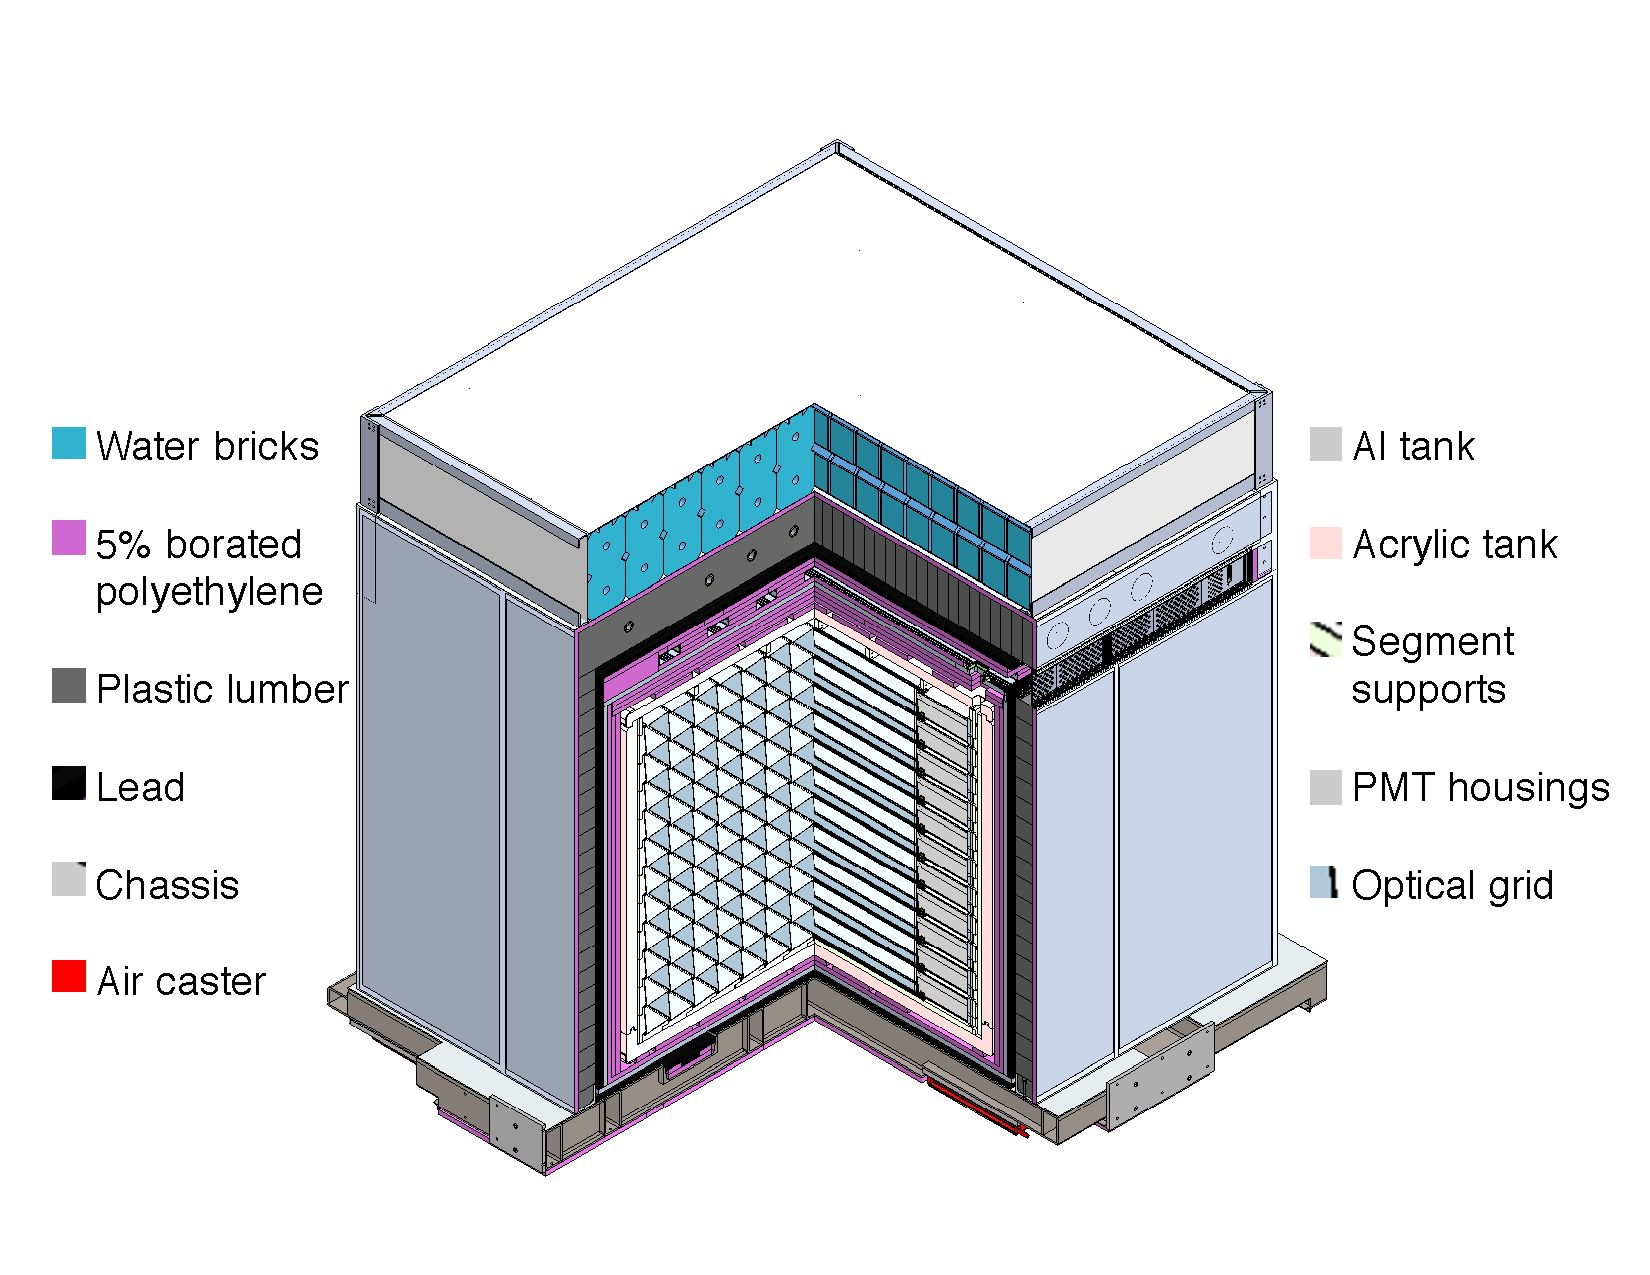
\includegraphics[trim = 0cm 2cm 0cm 2cm, clip,width=0.6\textwidth]{Figures/DetectorDesign.pdf}
    \caption[The design of PROSPECT AD]{The design of PROSPECT AD consisting the inner detector and the shielding.
    The inner detector includes $^{6}$LiLS, the optical grid, photomultiplier tubes (PMTs), and the calibration system.
    }
    \label{fig:PROSPECT_AD}
\end{figure}

    The inner volume of the PROSPECT AD is optically segmented by a light weight optical grid subsystem~\cite{bib:prospect_og}.
    The optical grid consist of highly reflective carbon fiber backed separators dividing the LS volume into 14$\times$11 identical longitudinal segments. 
    The ends of each segments are enclosed by two diameter = 12.7~cm photomultiplier tubes (PMTs).
    The schematics of the PROSPECT AD inner volume is shown in Figure~\ref{fig:active_volume}.
    The segment with largest LS light yield is identified as the interaction point (x- and y-direction) of an incident particle.
    The readout of PMT housed in mineral-oil filled acrylic modules (PMT optical modules) on both sides of each segment, allowing for timing- and charge-based position reconstruction along the axis (z-direction) of each segment~\cite{bib:P50, bib:P20}.
    Hence, the optical grid made PROSPECT AD able to reconstruct incident particles' track and 3D position, which is an essential function for the cosmic ray rejection and the oscillation measurement in the baseline between 7~m to 9~m.
    
\begin{figure}[h]
    \centering
    %\vspace{0pt}
    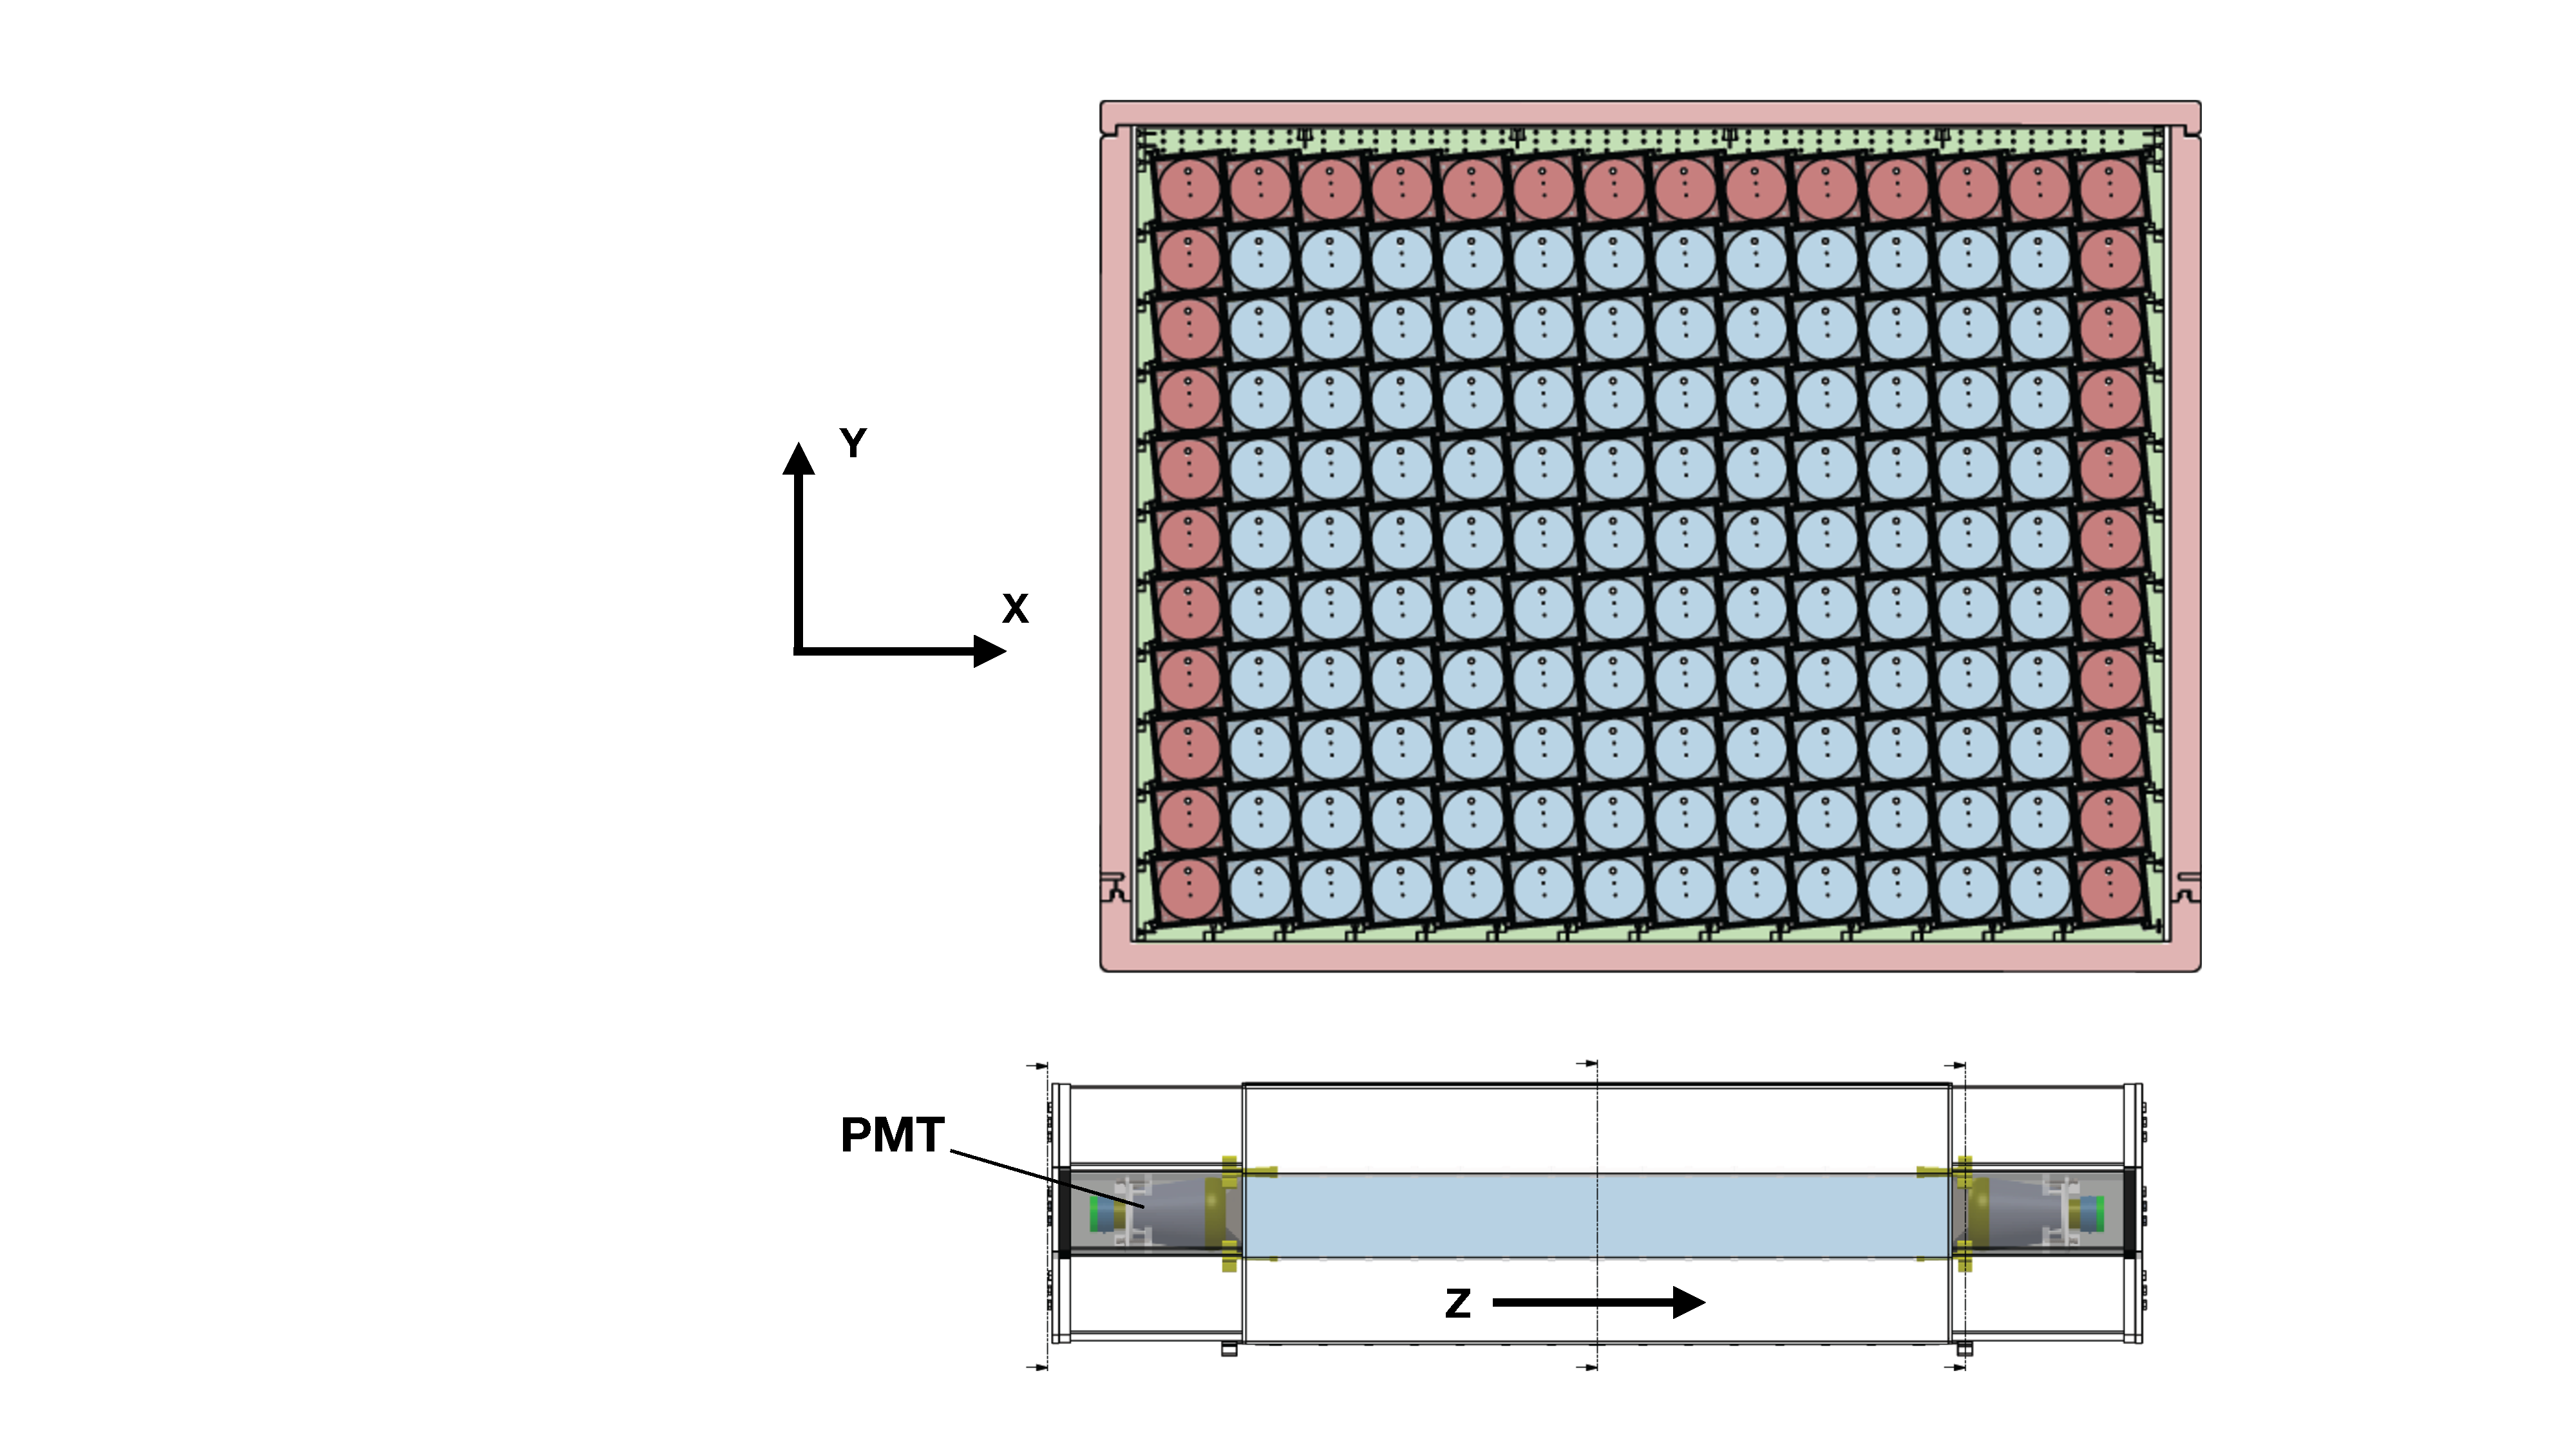
\includegraphics[width=0.7\textwidth]{Figures/PROSPECTAD_active.pdf}
    \caption[The inner volume of the PROSPECT AD]{The schematic of the inner volume of the PROSPECT AD.
    (Top) A side view to the X,Y plain of the AD, the red grids represent segments assembled with ET PMTs and the light blue grids represent segments with Hamamatsu PMTs.
    (Bottom) A schematic of a single segment.
    }
    \label{fig:active_volume}
\end{figure}

\Section{Antineutrino Detection}
\label{sec:detection}

\Subsection{IBD signature}
	Same as other reactor neutrino experiments, PROSPECT detect \nuebar through the detection of the positron and neutron produced in the IBD process
	\begin{equation}
        \nuebar + p \rightarrow n + e^+.
    \end{equation}	    
	The positron deposit its kinetic energy immediately in the LS by transferring the kinetic energy to molecular energy that generate scintillation light, whose process is described in detail in Chapter~\ref{Ch5}.
	After being losing most of its kinetic energy, positron-electron annihilation produces two 511~keV gamma toward two opposite directions. 
	The IBD produced neutron with keV scale kinetic energy is decelerated within 50~\textmu s until being captured by the nucleus in the LS. 
	The main neutron capturing isotope in the PROSPECT AD is $^6$Li with more than 80\% of neutron capture fraction.
	The $n$-Li capture process,
	\begin{equation}
       	n+^6\textrm{Li} \rightarrow \alpha + ^3\textrm{H},
    \end{equation}
    brought an advantage for PROSPECT that the event signature includes only the recoil of $\alpha$ and $^3$H nuclei without energy loss. 
    On the contrary, most of the historical reactor neutrino experiments utilizing Gd as the neutron capture solvent have to tag the neutron signal as a cascaded of $\gamma$ ray with total energy of approximately 8~MeV.
 	The scintillation signal of the IBD produced positron and its annihilation gammas is detected in 10~ns scale after the IBD process, followed by the $\sim$50~\textmu s delayed neutron capture signal. 
 	Hence, the positron and neutron signals are referred as prompt and delayed signals, respectively.
	A schematic of the IBD signals in PROSPECT is shown in Figure~\ref{fig:IBDscheme}.
\begin{figure}[h]
    \centering
    %\vspace{0pt}
    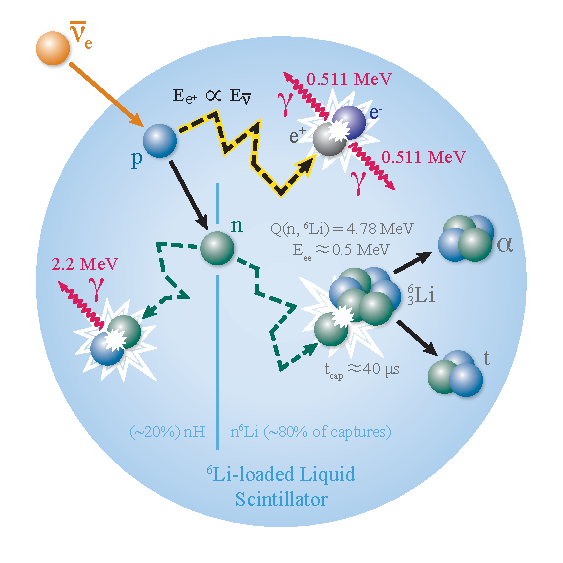
\includegraphics[width=0.7\textwidth]{Figures/IBDSchematic.pdf}
    \caption[IBD detection schematic]{The schematic of the IBD detection in PROSPECT AD.]
	An IBD event is tagged with the time coincidence between the positron and the neutron events.
	The positron deposits its energy and annihilate in $\sim$10~ns after IBD process.
	Wthin $\sim$50~\textmu s after the IBD process, the neutron is mainly captured by $^6$Li, generating $\alpha$ and tritium with total kinetic energy of 4.78~MeV (0.55~MeV electron equivalent).}
    \label{fig:IBDscheme}
\end{figure}

\Subsection{Prompt and Delayed Signal Discrimination}
	PROSPECT discriminate the prompt and delayed signal with PSD. 
	The pulse shape of scintillation light in EJ-309 contains short lived and long lived fluorescence components whose fractions in the light pulse are dependent on the $dE/dx$ of exciting particle. 
	Since the $dE/dx$ of charged nuclei is greater than the positrons and electrons, a significant difference of pulse shapes between the prompt and the delayed signals is shown as Figure~\ref{fig:PSD}.
	\begin{figure}[h]
    \centering
    %\vspace{0pt}
    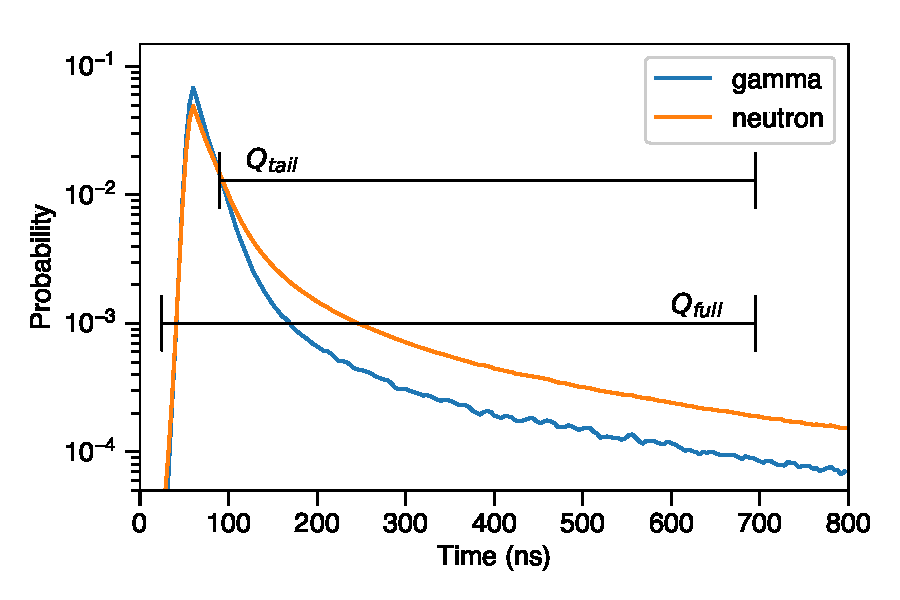
\includegraphics[width=0.6\textwidth]{Figures/PSD.pdf}
    \caption[Pulse shape difference]{
	An example of the different pulse shape between gamma-ray like signal and neutron like signal.
	}
    \label{fig:PSD}
	\end{figure}
	For the ease of signal discrimination, a PSD parameter is defined as the tail fraction of the pulse integral, 
	\begin{equation}
       	\textrm{PSD} = \frac{Q_\textrm{tail}}{Q_\textrm{full}}.
    \end{equation}
    With the event selection based on the reconstructed energy, timing and PSD value of a pulse, clear signal types can be distinguished as shown in Figure~\ref{fig:PSDvEvT}.
    	\begin{figure}[h]
    \centering
    %\vspace{0pt}
    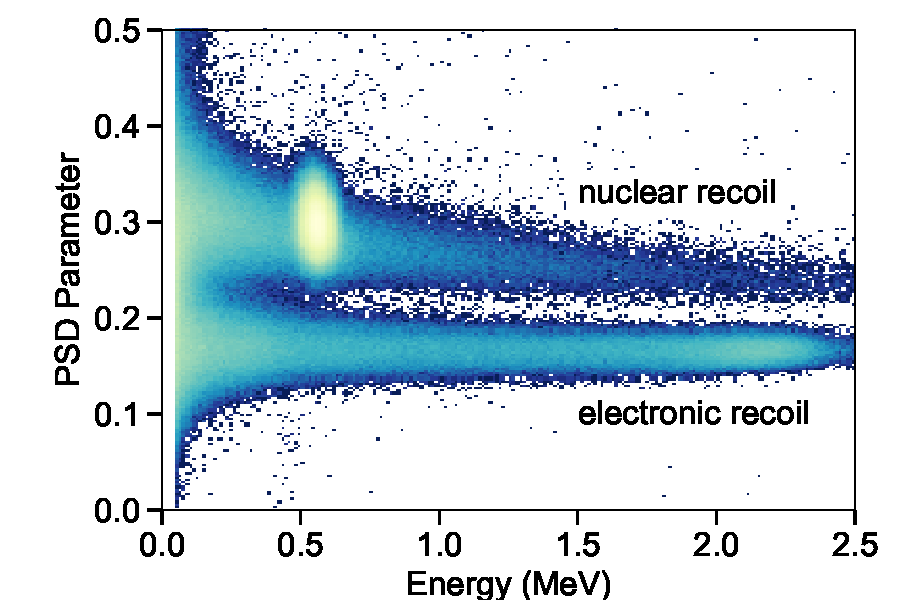
\includegraphics[width=0.48\textwidth]{Figures/PSDvE.pdf}
    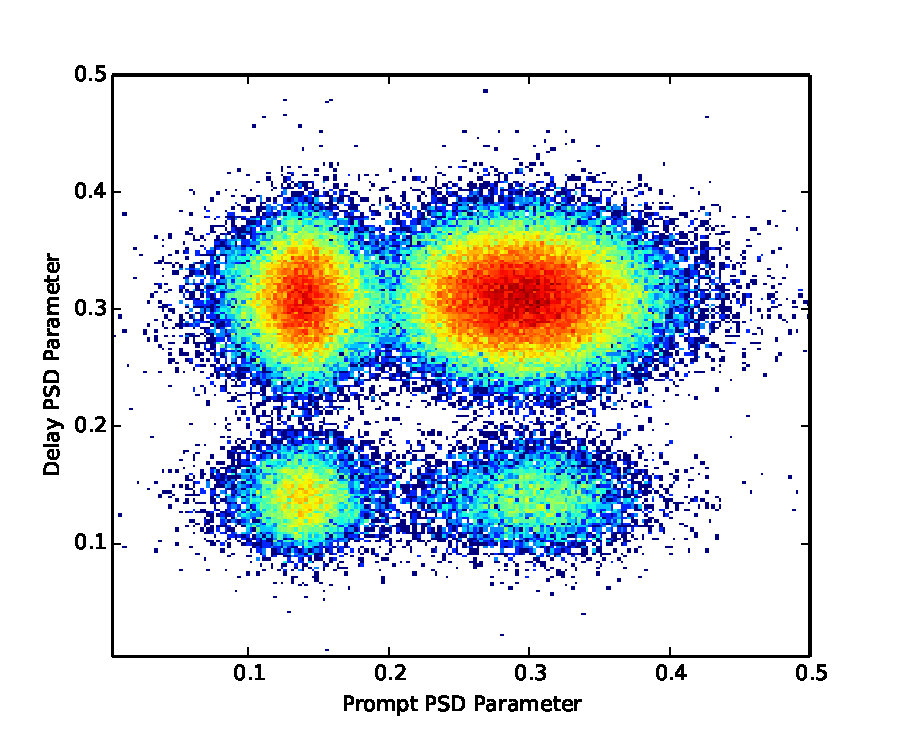
\includegraphics[width=0.48\textwidth]{Figures/PSDvT.pdf}
    \caption[Event selection based on PSD]{
    	(Left) The distribution of $^{252}$Cf neutron and gamma events in a energy and PSD parameter space.
    	A well constrained distibution of $n$-Li capture can be seen at the low energy high PSD spot.
    	(Right) The distribution of prompt-delay pair event in the PSD and time coincidence parameter space, where the top left spot is the distribution of IBD candidates.
	}
    \label{fig:PSDvEvT}
	\end{figure}
	
\Subsection{Energy and Position Reconstruction}
	PROSPECT AD is a segmented detector where particles with enough energy can travel through multiple segments.
	The energy of a particle deposit in each segment is reconstructed with respect to the light collected by the PMTs on both ends.
	When both PMTs of a segment is triggered to collect light, the recorded signal by the segment is referred as a \textit{hit}.
	An event \textit{cluster} is defined as a group of hits in a 20~ns time interval between every two hits. 
	The reconstructed energy of a particle is the sum of energy deposit in all segments of a cluster, as illustrated in Figure~\ref{fig:ClusterScheme}.
	The reconstructed event vertex's (X, Y) position is defined as the location of the segment with largest energy deposition in a cluster.
\begin{figure}[h]
    \centering
    %\vspace{0pt}
    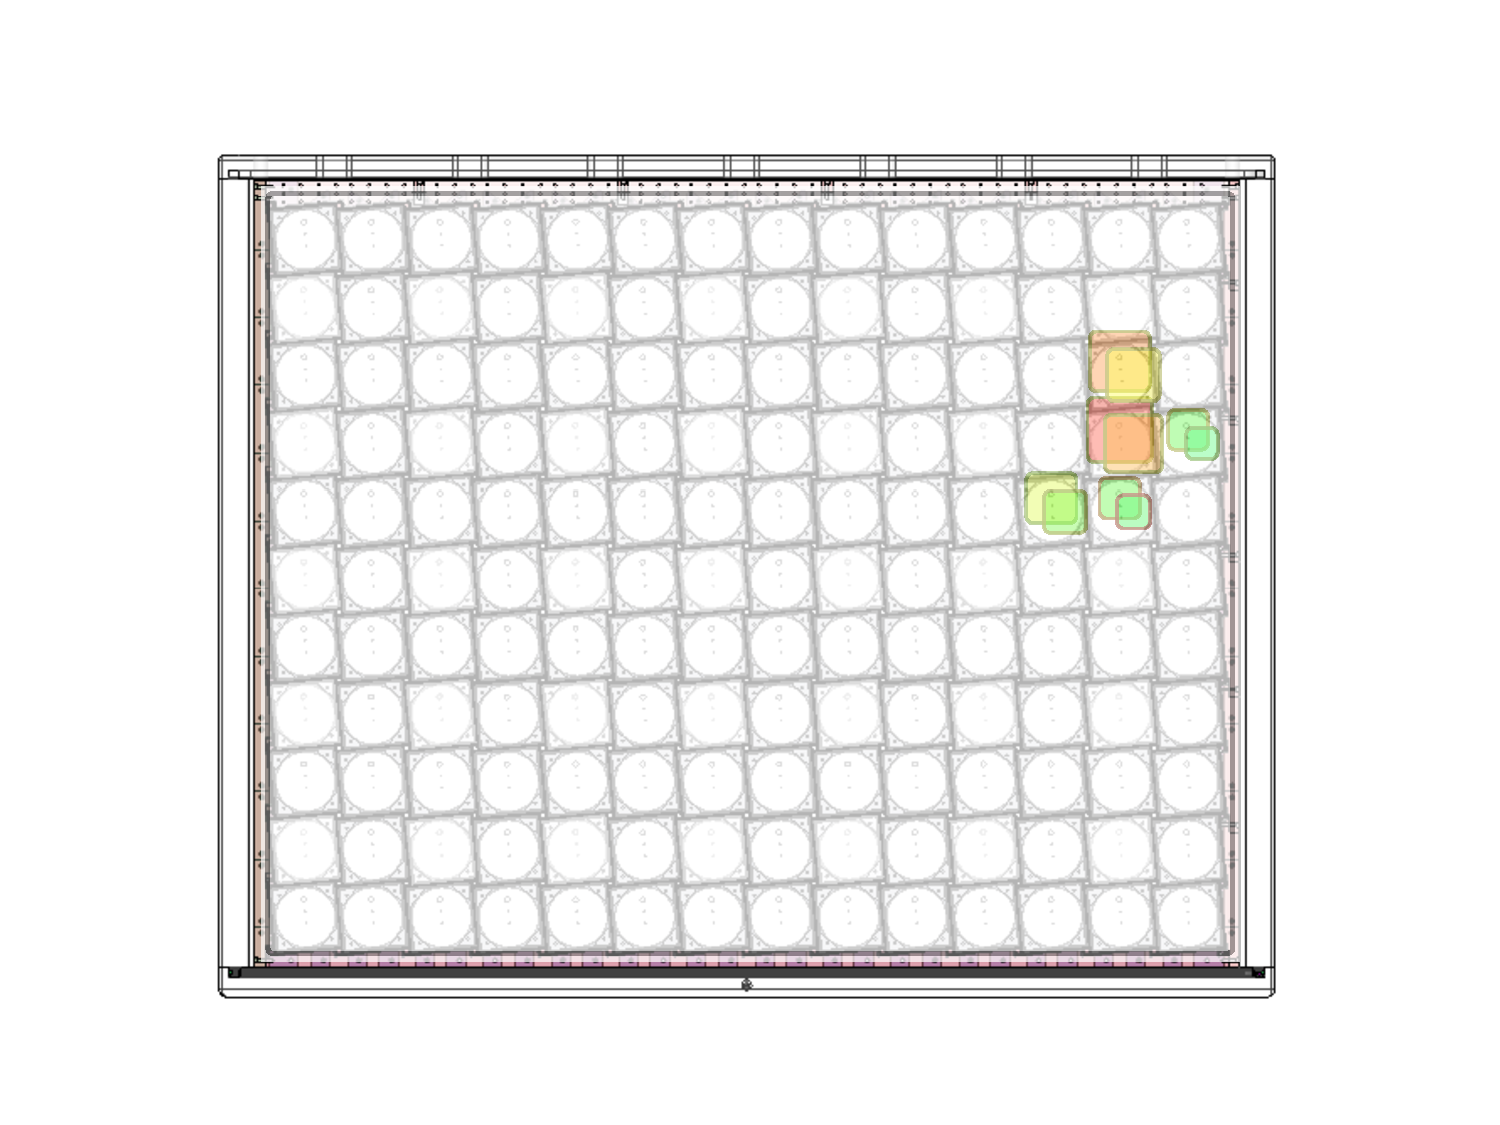
\includegraphics[width=0.6\textwidth]{Figures/ClusterScheme.pdf}
    \caption[An illustration of an event cluster]{
	An illustration of an event cluster. The colored segments are segments collected scintillation light within a clusters time window.
	The reconstructed energy of this event is the summed energy detected by each segment hit in this cluster.
	The size and color of each colored box is correlated to the light collected in each PMT.
	The reconstructed positron is in the segment with largest light collection.
	}
    \label{fig:ClusterScheme}
\end{figure}
	
	An event vertex's Z position is reconstructed based on the charge and timing difference between the pair of PMTs' light signal.
	The schematic of a single segment light collection is shown in Figure~\ref{fig:Zreconstruction}.
	Because of the light attenuation in the LS, the light collection by a PMT at one end decreases exponentially with increasing distance from that PMT to the vertex, resulting in the segments total light collection non-uniformity along the Z direction.
	The detection timing difference between the PMTs is also dependent on the Z position, making it a useful tool in Z positrion reconstruction.
	Further discussion about the Z position calibration is detailed in Chapter~\ref{Ch6}.
	
\begin{figure}[h]
    \centering
    %\vspace{0pt}
    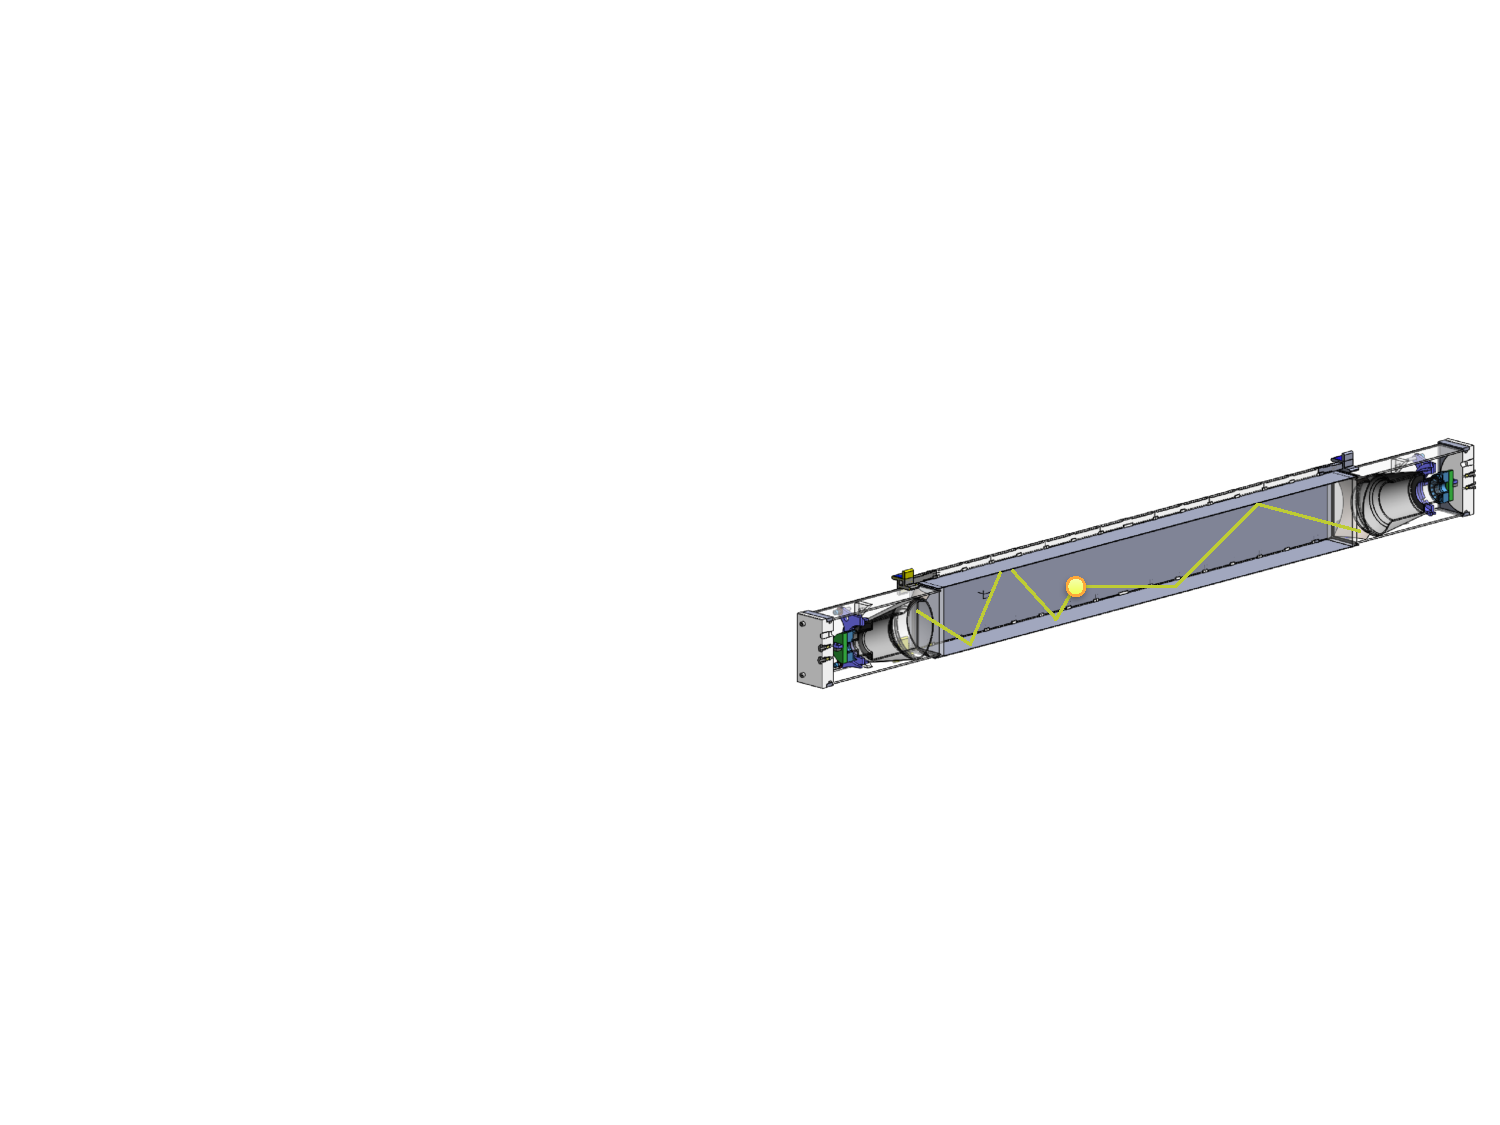
\includegraphics[width=0.6\textwidth]{Figures/Z_reconstruction.pdf}
    \caption[A schematic of a single segment light collection ]{
	A schematic of the light collection within one segment. 
	When scintillation light was generated from an incident particle particle, the light is constrained in the segment by the specular reflective separators.
	The two PMTs on the ends detect different light and at different time with respect to the vertex location.
	}
    \label{fig:Zreconstruction}
\end{figure}
	


\Chapter{Detector Research and Development}
\label{Ch4}

The research and development (R\& D) of PROSPECT detector began in 2014.
Multiple prototypes were assembled to in the R\& D phase to develop and demonstrate a variety of detector design.
In this phase, many candidate materials were tested. 
The time line of the PROSPECT R\& D is shown in Table~\ref{tab:Prototypes}

\begin{sidewaystable}[h!]
    \centering
    \caption[PROSPECT R\& D and construction phases]{PROSPECT R\& D and construction phases.}
    \begin{tabular}{cccc}
        Phase & Time & Goal & Reference \\
        \hline
        \hline
        0.1~liter prototype  & Aug. 2014 & DAQ, LS performance &\\
        2~liter prototype   & Dec. 2014 to Mar. 2015 & Background survay, shielding & \cite{bib:prospect_background}\\
        20~liter prototype   & Mar. 2015 to Aug. 2016 & Single segment performance & \cite{bib:P20} \\
        50~liter prototype   & Jan. 2016 to Mar. 2019 & Two segment event reconstruction, detector stability & \cite{bib:P50} \\
        \hline
        LS fabrication & Jan. 2016 to Oct. 2017 & Fabrication  & \cite{bib:P50} \\
        PMT module assembly & Jan. 2016 to Mar. 2019 & Two segment event reconstruction, detector stability & \cite{bib:P50} \\
        Optical grid component fabrication & Jan. 2016 to Mar. 2019 & Two segment event reconstruction, detector stability & \cite{bib:P50} \\  
        \hline
		Detector assembly & Jan. 2016 to Mar. 2019 & Two segment event reconstruction, detector stability & \cite{bib:P50} \\       
        Detector commissioning & Jan. 2016 to Mar. 2019 & Two segment event reconstruction, detector stability & \cite{bib:P50} \\ 
        \hline 
        Data acquisition & Jan. 2016 to Mar. 2019 & Two segment event reconstruction, detector stability & \cite{bib:P50} \\ 
        \hline
    \end{tabular}
        \label{tab:Prototypes}
\end{sidewaystable}

\Section{Prototype Research}
	
\Section{Optical Grid}
\label{sec:OG}

\Section{Calibration System}

\Section{Detector Construction and Commissioning}

\Section{Data Acquisition}

\Chapter{Monte-Carlo Simulation for PROSPECT}

\Section{Particle Interaction Simulation}

\Section{DAQ Pulse Simulation}

\Chapter{Monte-Carlo Simulation for PROSPECT}

Monte-Carlo Simulation for PROSPECT is a key portion of the analysis.


\Section{Particle Interaction Simulation}

\Section{DAQ Pulse Simulation}

\Chapter{Detector Calibration}
\label{Ch6}

\Section{Introduction}
\label{sec:intro}
The PROSPECT reactor antineutrino measurement relies on the reconstruction of the prompt energy spectrum of IBD events, model independent spectral comparison between baselines for oscillation analysis, and the data-model comparison of reconstructed prompt spectrum.

The reconstructed energy of particles in the detector is naturally different from the energy deposit by the particles because of detector geometry, imperfection and nonlinearity. 
It is vital to characterize the detector response with correct detector structure, nonlinearity of energy response and energy resolution to
\begin{itemize}
    \item Supply accurate detector response model through MC with correct key values.
    \item Quantify the systematic uncertainty in energy response. 
\end{itemize}

In this study, the gamma sources, neutron source calibration and ambient data calibration were performed to PROSPECT Antineutrino Detector (AD). 
These calibration helped characterize the absolute detector response, including nonlinearty induced by the Birks' law quenching and Cherenkov radiation of scintillator, the energy resolution that is contributed by the detector geometry and photon statistics, and absolute energy scale caused by calibration presumption of n-capture reconstructed energy. 
In addition, necessary detector geometry corrections were implemented, with respect to physical measurements on detector material and dimensions, to enhance data-MC agreement in gamma collection.
At last, the combined fit of all calibration data to Monte-Carlo (MC) simulation was made to constrain  the energy resolution and nonlinearity model.


\Section{Calibrations}
Three calibration campaigns were organized in 2018 to characterize the detector response.
The sources available in each campaign are shown in Table~\ref{tab:src_table}.
Each radioactive source was sealed in an aluminum capsule, then inserted through calibration tube by time belt and deployed close to the center of detector.
Once in position, each $gamma$ calibration run last for 10 minutes, most of $^{252}$Cf and AmBe calibration run last for more than 1 hour because of relative lower activity.

\begin{sidewaystable}[h]
    \centering
    \caption{Calibration source utilized}
    \begin{tabular}{cccc}
        Source & Decay Type & Energy[MeV] & Time in 2018\\
        \hline
        \hline
        $^{137}$Cs  & $\beta^-$   & $0.662$ (de-excitation $\gamma$) &Apr, Aug, Dec\\
        $^{22}$Na   & $\beta^+$   & $1.274$ (de-excitation $ \gamma$) + $2\times0.511$ (annihilation $\gamma$) &Apr, Aug, Dec\\
        $^{60}$Co   & $\beta^-$   & $1.17 + 1.33$ de-excitation $\gamma$ &Apr, Aug, Dec \\
        \hline
        $^{252}$Cf  & SF   & 2.223 (n-H capture de-excitation $\gamma$) &May, Aug, Dec \\
        \hline
        AmBe	& $^{9}$Be($\alpha$, $n$)$^{12}$C	& 4.4~MeV  de-excitation $\gamma$, $\sim$1~MeV nucleon recoil & Dec \\
        \hline
        $^{12}$B	&	$\beta^-$ & 3~MeV to 13.4~MeV & Ambient data \\
        \hline
    \end{tabular}
        \label{tab:src_table}
\end{sidewaystable}

During data acquistion, PMT trigger thresholds, refered as the Zero Length Encoding (ZLE) thresholds, were set to reduce the electronic noise in each DAQ channel.
The ZLE threshold is a pulse height threshold requires the pulse from both PMTs in each cell exceed a specific height to record event position and energy in the segment.
During the gamma and neutron calibrations, the ZLE thresholds were 10 and 20 ADC units respectively, equivalent to 40 to 80 keV.
The light collection varies through out the detector because of detector nonuniformity and LS attenuation length.
Because the time dependence of the PMT gain and scintillation light yield also exist in PROSPECT AD, the ZLE threshold can induce non-uniform reconstructed energy scale based on the position and time of the incident particle.
Hence, a 90~keV threshold of reconstructed energy for each segment was manually set to resolve this non-uniformity by cut the hits with reconstructed energy lower than 90~keV, thus ensure the uniformity of the lower energy event selection doc90keV. 

To unpack and analyze the calibration data, the PROSPECT-2x analysis package was used to reconstruct the gamma energy of clusters in the full detector and the Compton scattering energy deposited in single segments. 
The reconstructed energy resolution is mainly dependent on the photostatistics of events. 
Therefore, the energy resolution varies with respect to the non-uniformity of light collection among cells and evolve during the data acquisition period.
During the data unpacking and analysis, each hit of a cluster is artificially smeared based on the lowest photostatistics, 325~PE/MeV found in current data release, as shown in Figure~\ref{fig:PEvTime}.

\begin{figure}[ht]
\centering
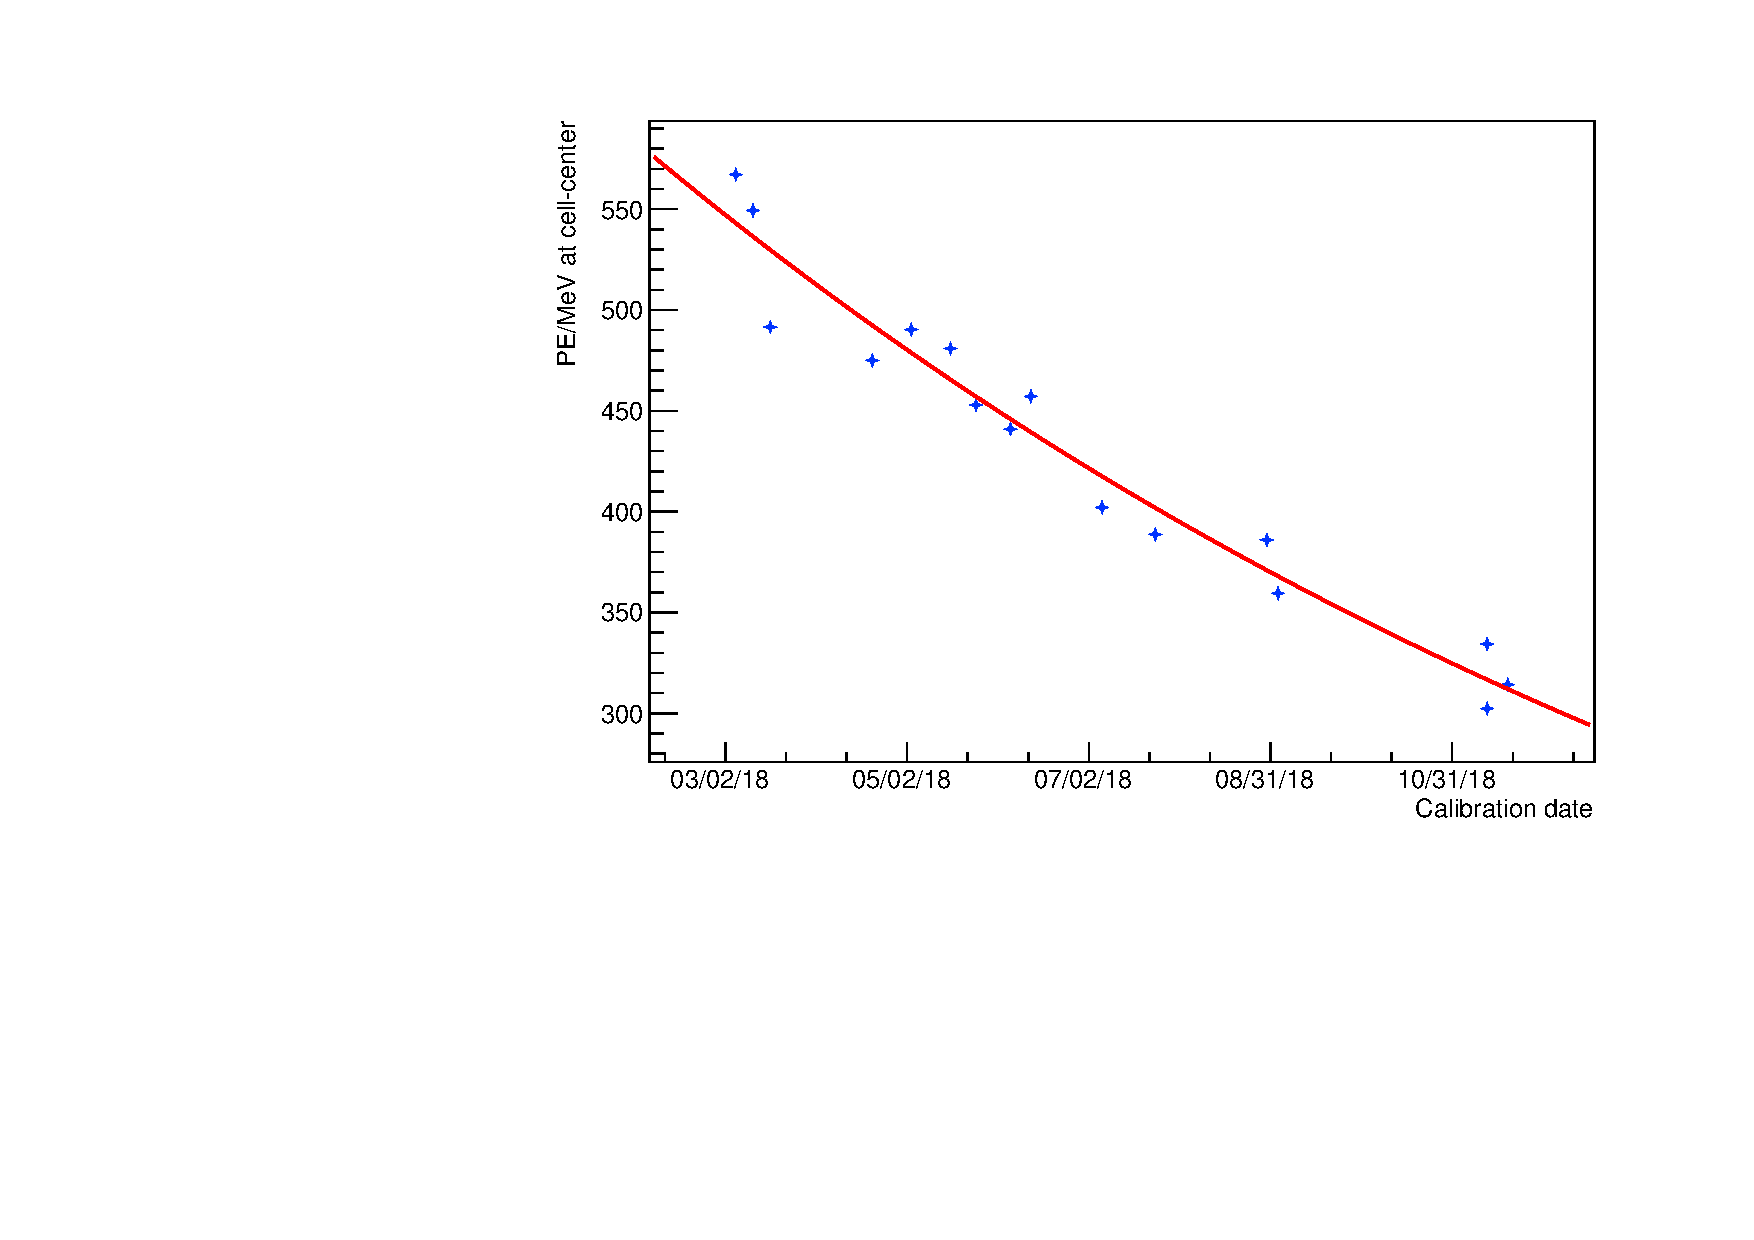
\includegraphics[width=0.6\textwidth]{Figures/PEvsTime.pdf}
\caption{PE per MeV during the 2018C data acquisition period. The fitted function suggests 346$\pm$17 PE/MeV at the end of the period.}
\label{fig:PEvTime}
\end{figure}

\Subsection{Energy Reconstruction}
For the gamma source calibration, including the $^{137}$Cs, $^{22}$Na and $^{60}$Co calibrations, the gamma-like events are selected within the 3$\sigma$ range of the PSD distribution of electrons.
Specific background data was taken for background subtraction.

To reconstruct the the $n$-H capture gamma energy, the time coincidence between the prompt $\gamma$-ray (3 MeV to 15 MeV) emission from the $^{252}$Cf neutron source and the delayed de-excitation gamma from $n$-H captures was used to select the $n$-H event.
In the event selection, the ionization events after 0 to 200 $\mu s$ from the prompt gamma signal were tagged as correlated events, while the events -1200 to -200 $\mu s$ before prompt gamma are accidental.
The $n$-H $\gamma$ spectrum is measured by subtracting the correlated events in background data.
The calibration spectra is shown in Figure \ref{fig:gammacalib}.

\begin{figure}[ht]
\centering
\subfigure[The gamma energy distribution from $^{137}$Cs calibration.]{\label{fig:caliba}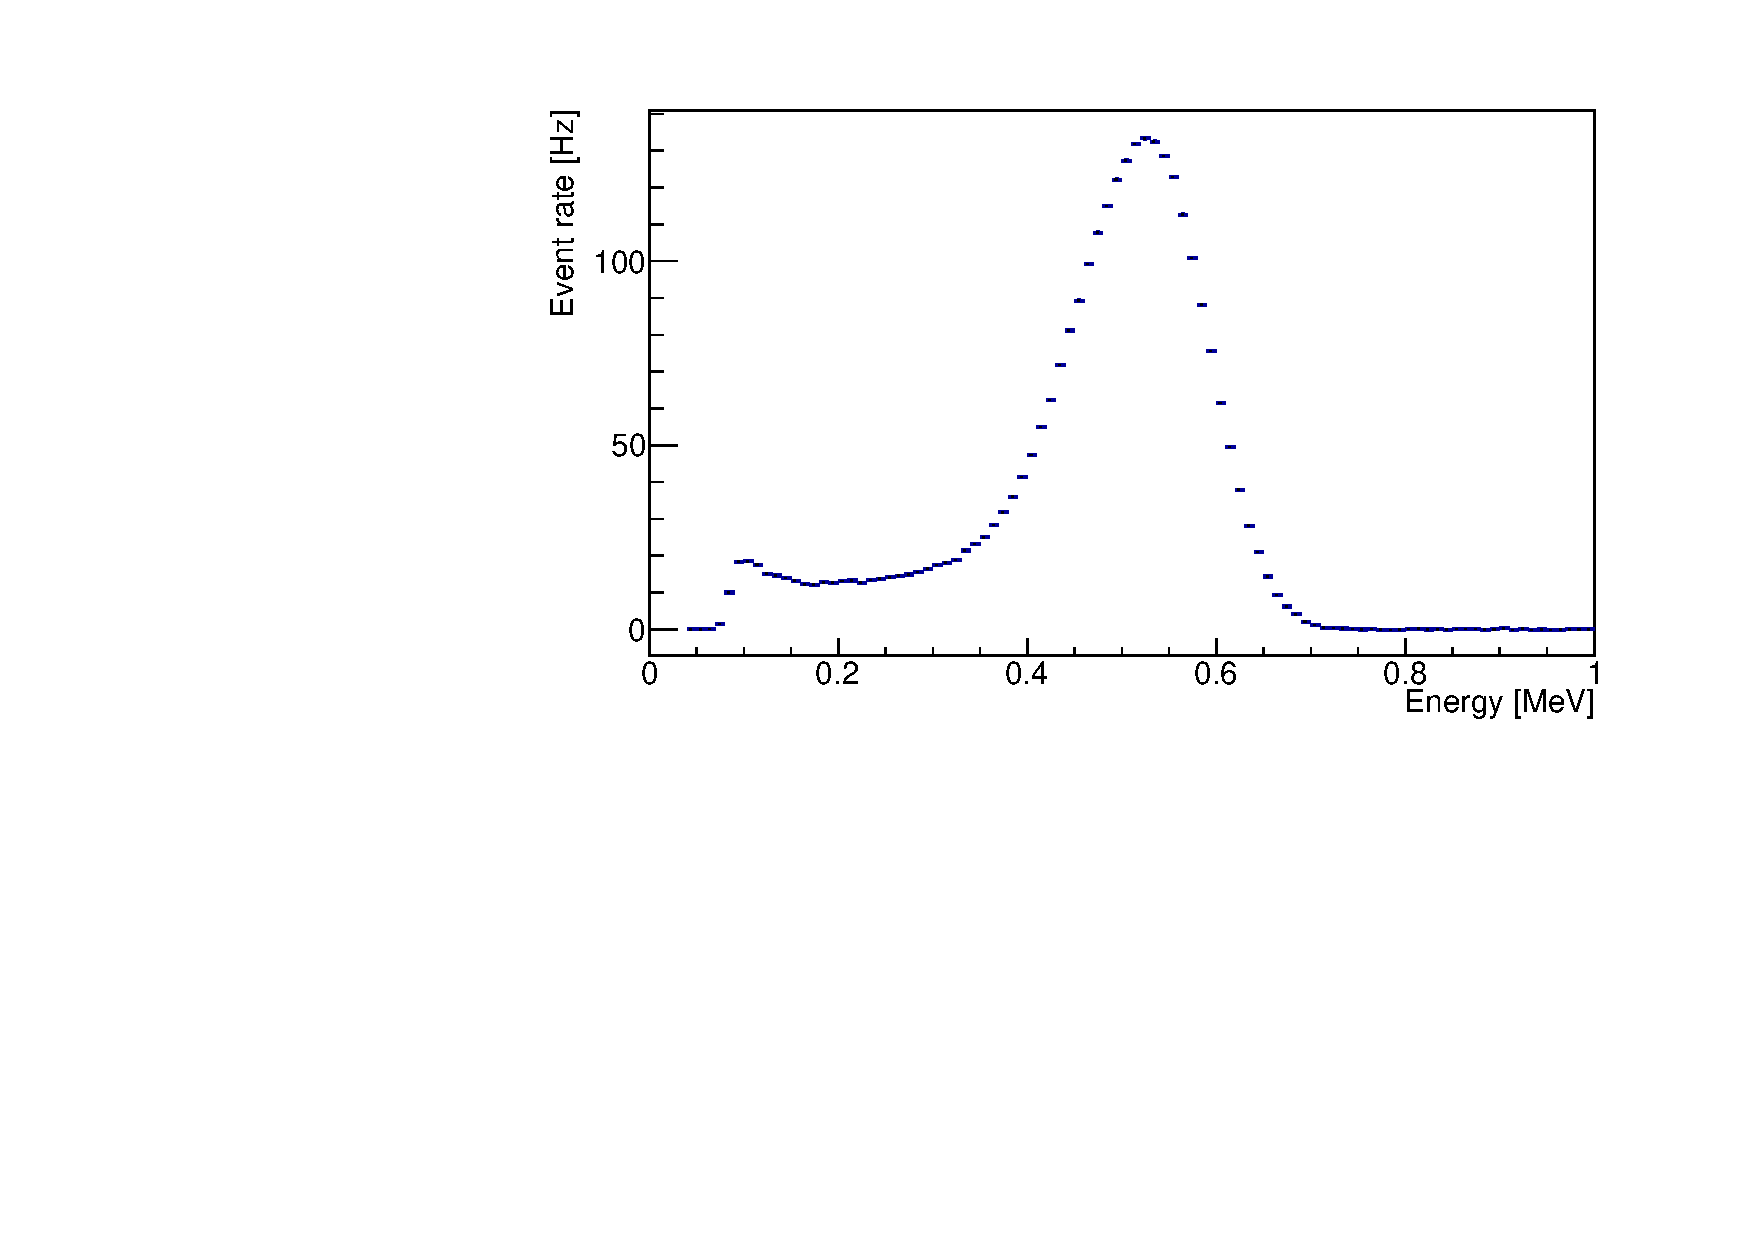
\includegraphics[width=60mm]{Figures/Cs137smear85.pdf}}\quad
\subfigure[The gamma energy distribution from $^{22}$Na calibration.]{\label{fig:calibb}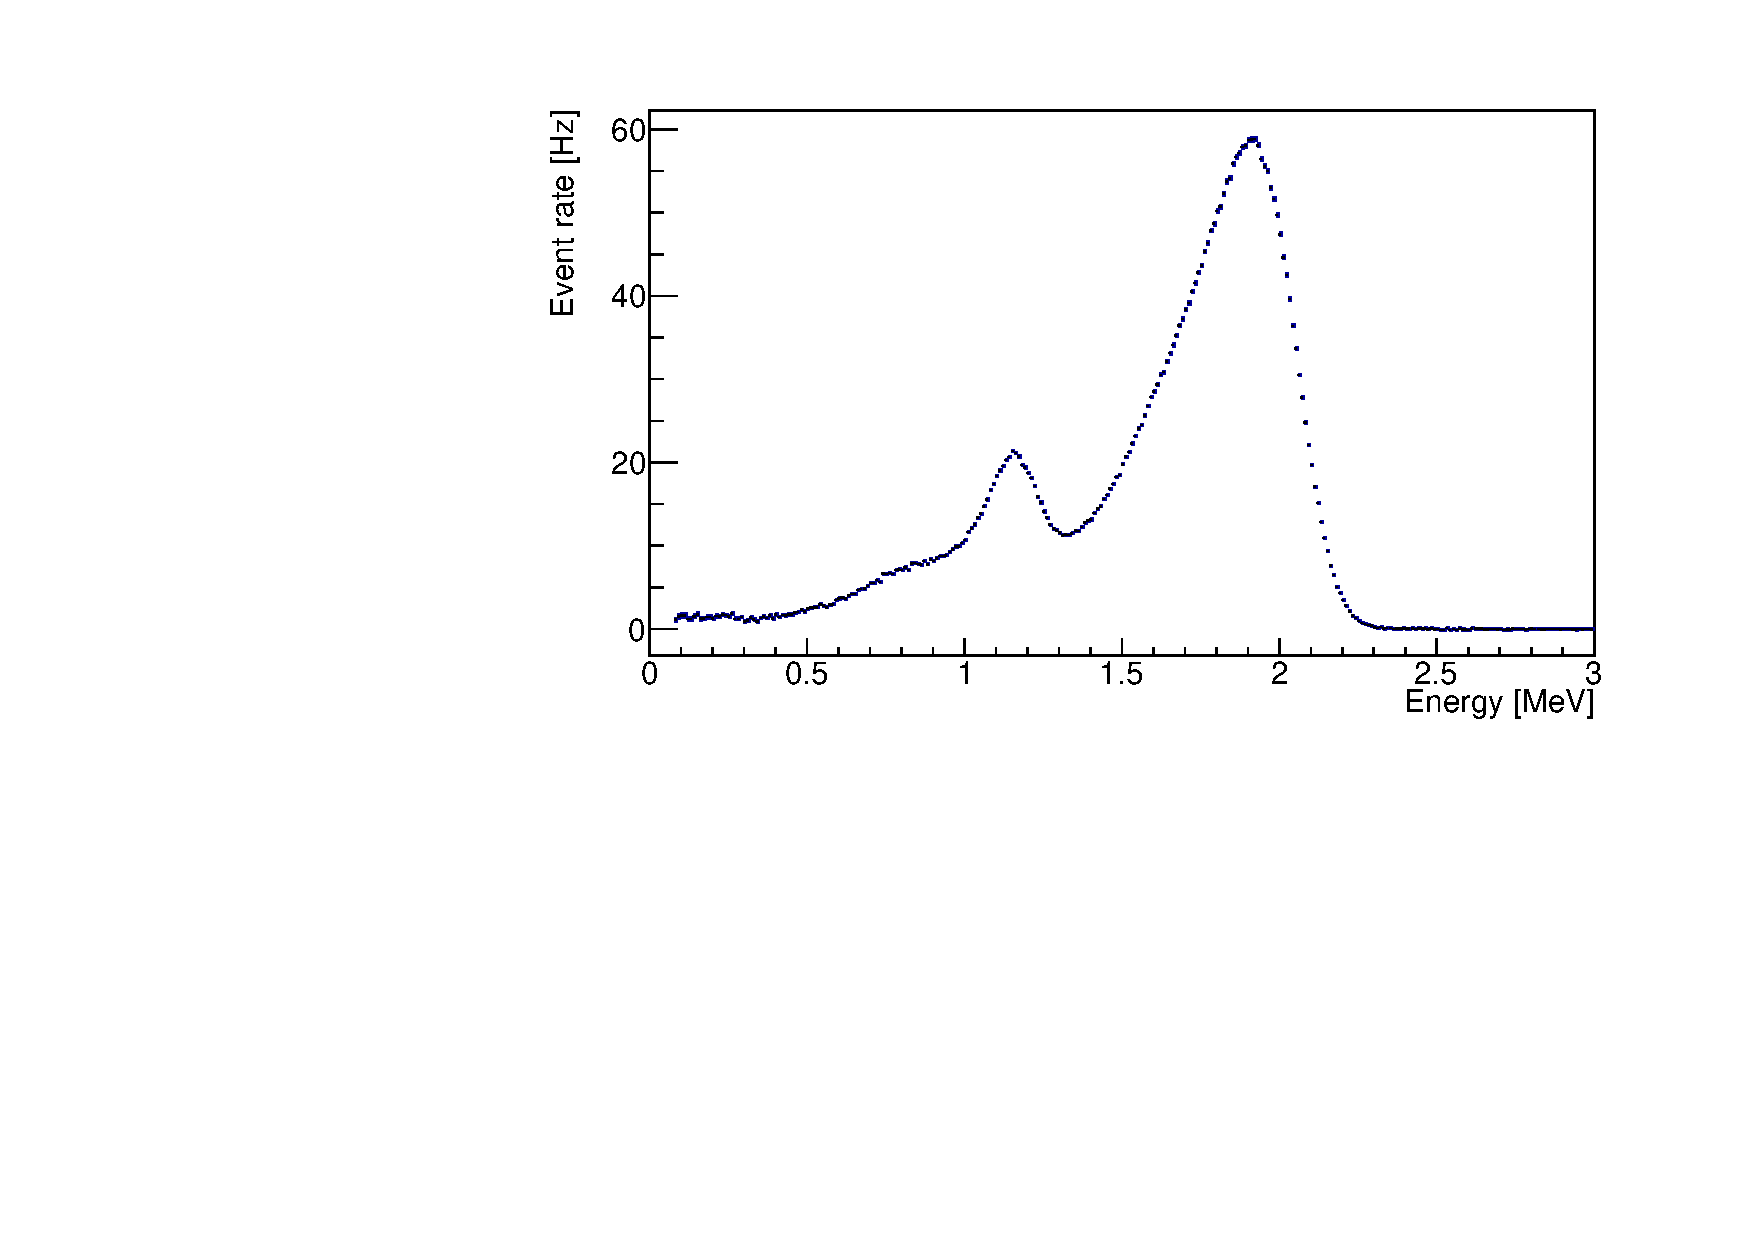
\includegraphics[width=60mm]{Figures/Na22smear85.pdf}} \\
\subfigure[The gamma energy distribution from $^{60}$Co calibration.]{\label{fig:calibc}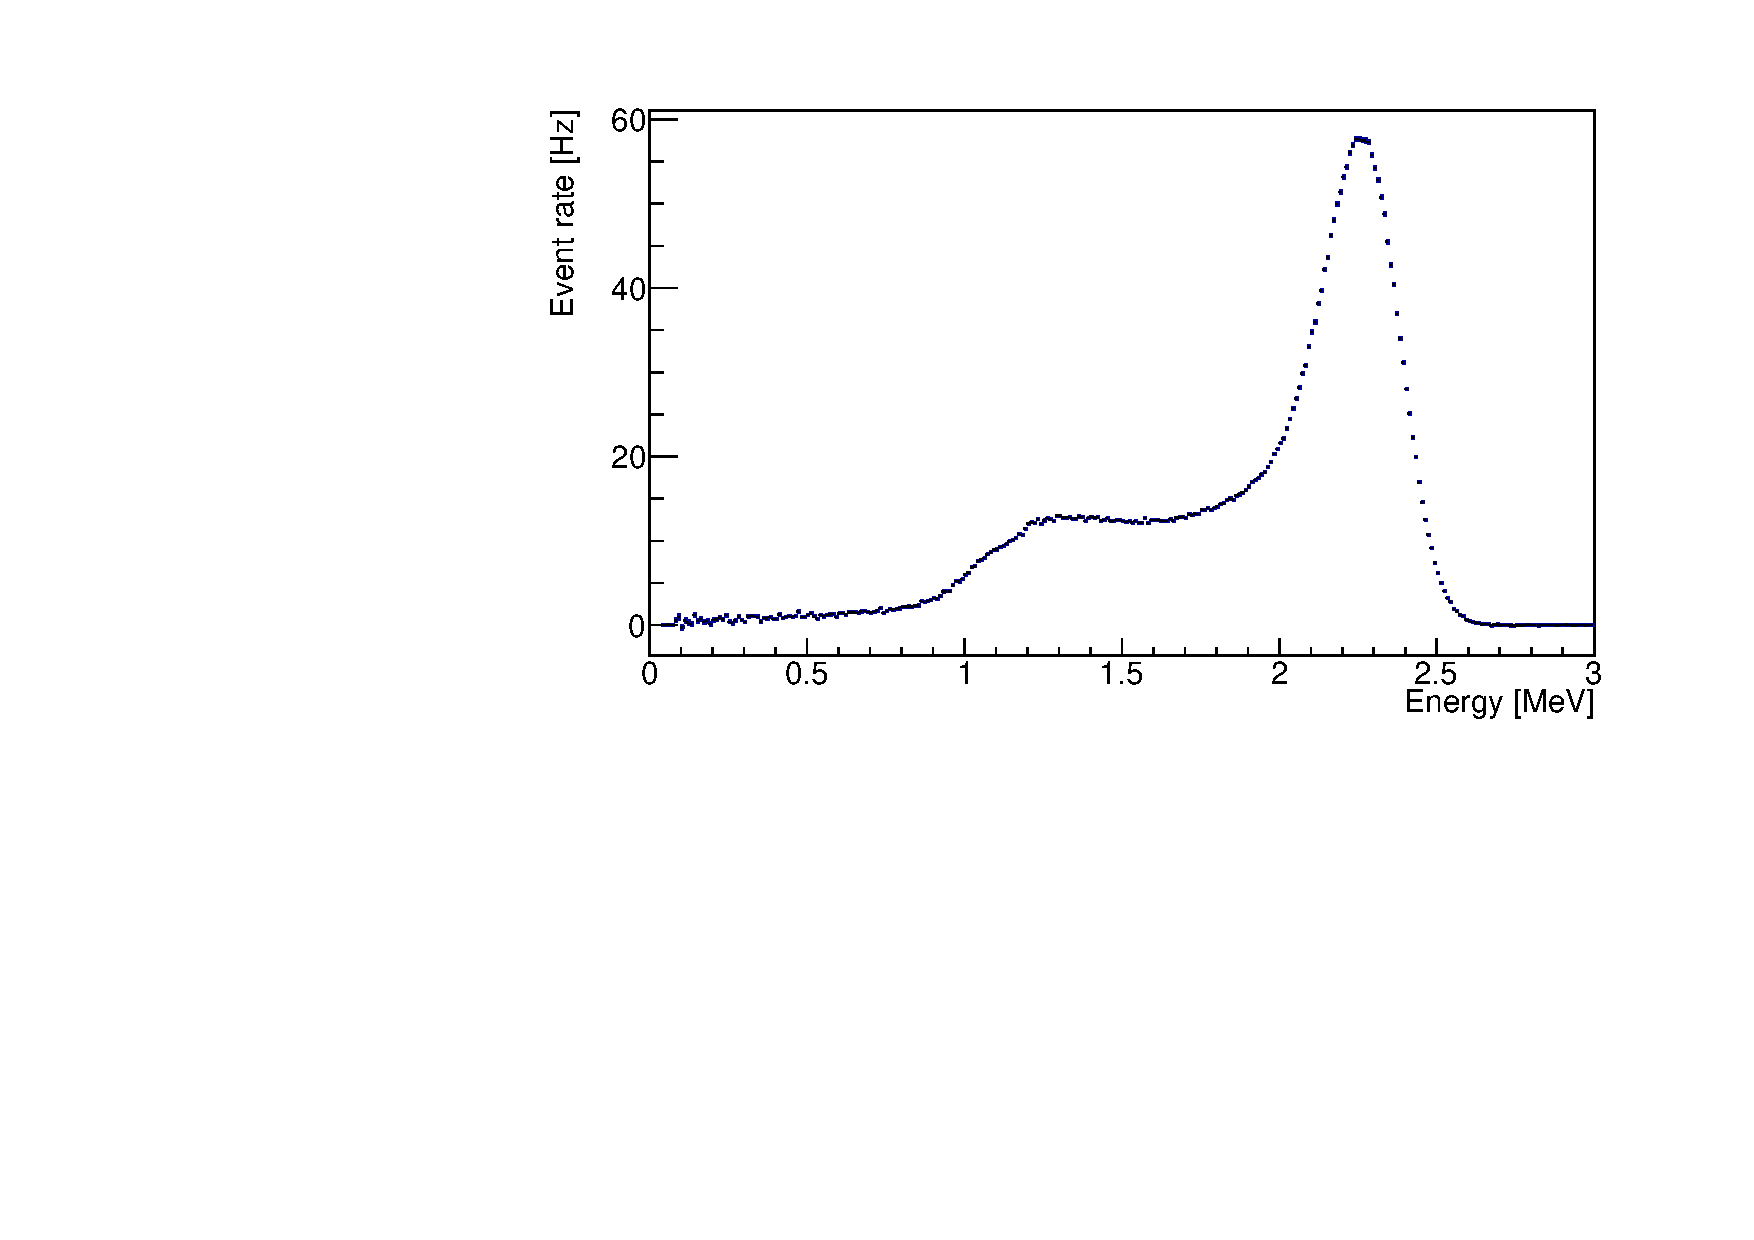
\includegraphics[width=60mm]{Figures/Co60smear85.pdf}} 
\subfigure[The gamma energy distribution from neutron captured by hydrogen.]{\label{fig:calibd}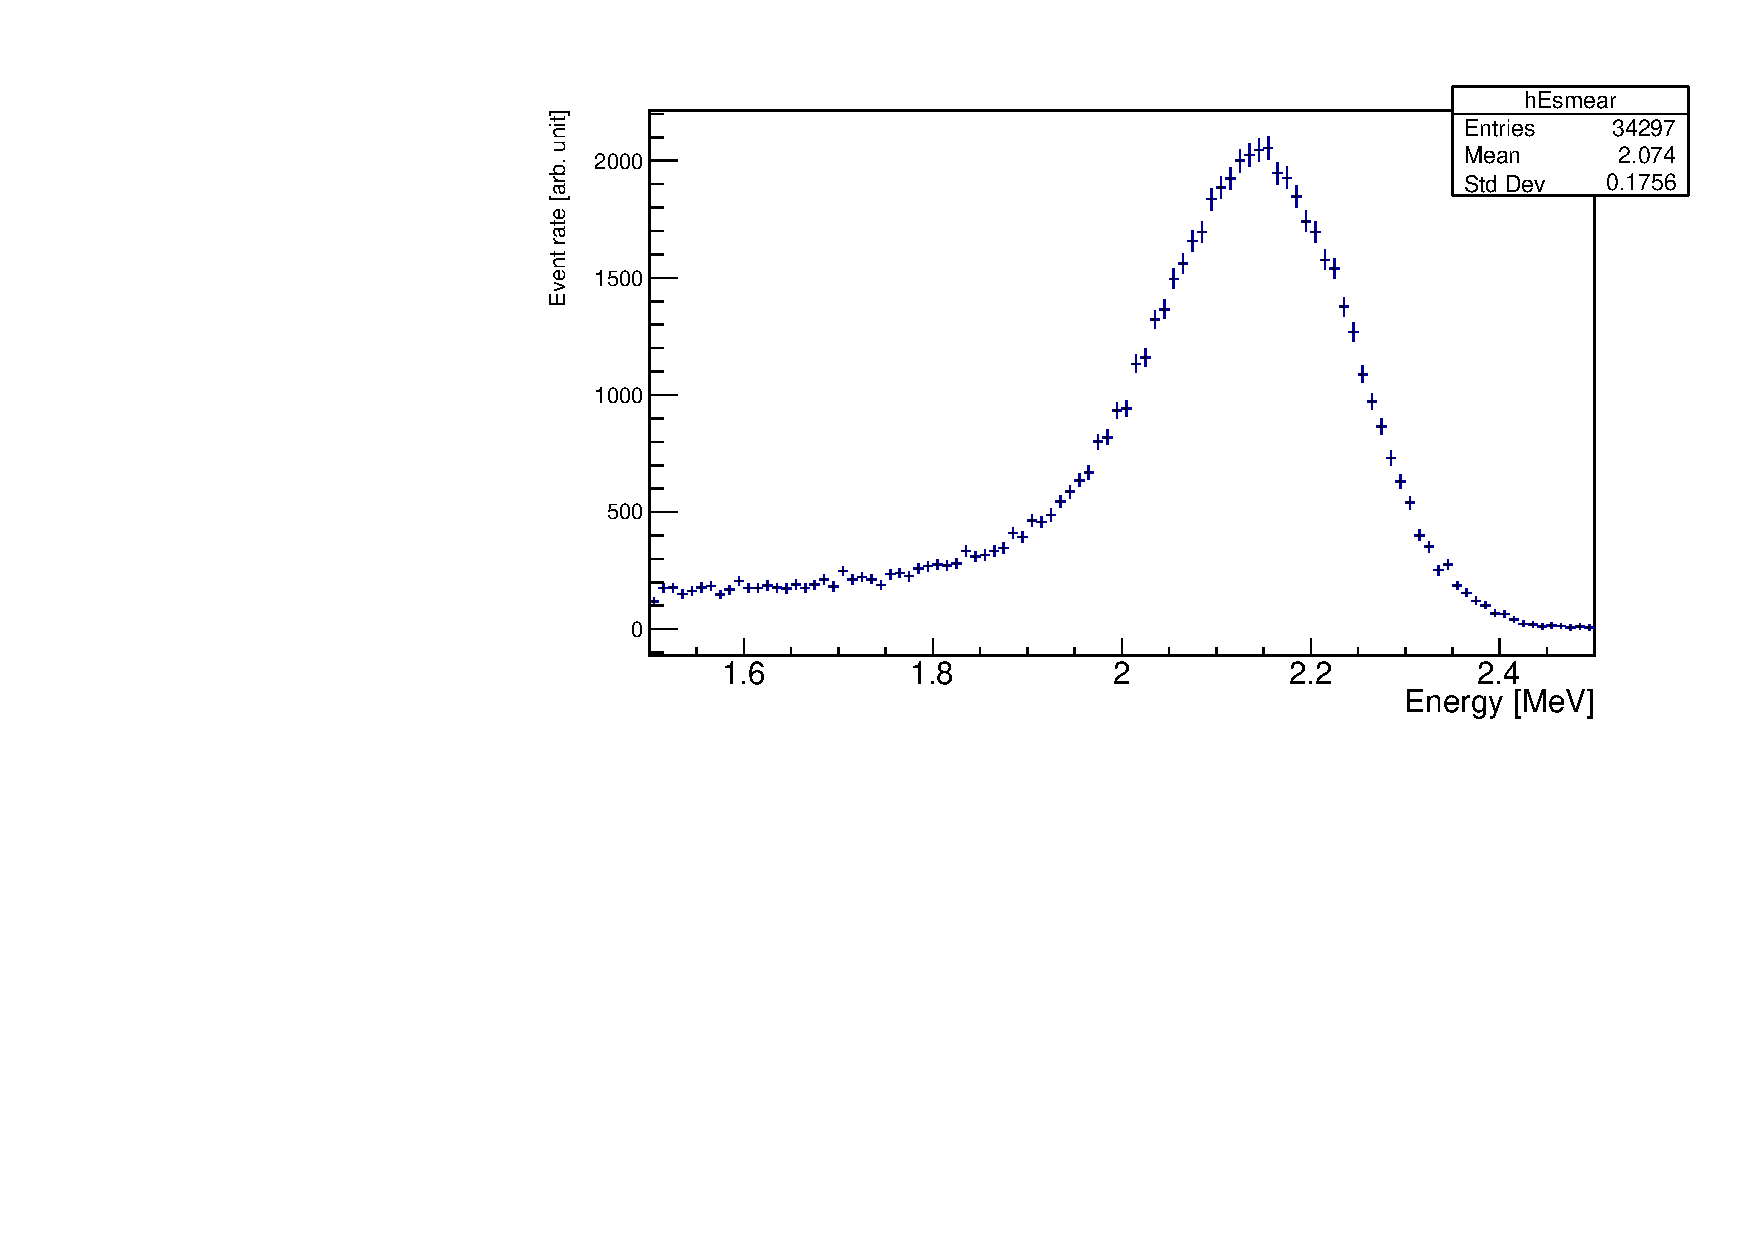
\includegraphics[width=60mm]{Figures/Cf252smear85.pdf}}
\caption{The gamma spectra of calibration sources.}
\label{fig:gammacalib}
\end{figure}

The $^{12}$B beta radiation is an ambient electron source that can be detected by PROSPECT AD
The $^{12}$B is mainly produced by cosmogenic neutron with $^{12}$C(n, p)$^{12}$B interaction, whose cross section is $\sim 0.01$ barn. 
Because of its $\beta$ energy disttribution covers the similar energy range to IBD energy of reactor antineutrino, it is a valuable calibration source to demonstrate the reconstructed energy scale of IBD events.
To select $^{12}$B events in PROSPECT, the time coincidence between prompt proton recoil and the $\beta$ dacay of $^{12}$B, as well as the prompt-delay distance was used. 
The prompt events includes single multiplicity recoil events in 0.7~MeVee to 10~MeVee range, followed by multiplicity $<$ 3  electron candidates with energy less than 20 MeV.
The event selection requires the delayed electron events to follow the single recoil event in 3~ms to 30~ms, while all electron events must be $<12$~cm from the recoil events and within the same fiducial volume as the IBD spectrum datasets.
In the procedure above, PSD was used to separate recoil and ionization events. The life time $^{12}$B decay was measured  $28.8\pm0.6$ ms that agreed with the norminal $29.14$ ms from ENSDF, shown in Figure \ref{fig:lifetime}. 
The prompt to delay distance is fitted with Gauss distribution, the best fit stardard deviation $\sigma_d$ = 2.91~cm, shown in Figure \ref{fig:distance}. 
The event selection $dz < 12$~cm is to minimize time variation of event selection since the position resolution of the detector evolves with time.
In 73~days reactor off data collection, there are $\sim 35300$ $^{12}$B decay counted in PROSPECT AD with S:B=0.87. 
The reconstructed spectrum of $^{12}$B electron is shown in \ref{fig:B12}.
\begin{figure}[h!]
\centering
\subfigure[The delay-prompt time difference of $^{12}$B candidates ]{\label{fig:lifetime}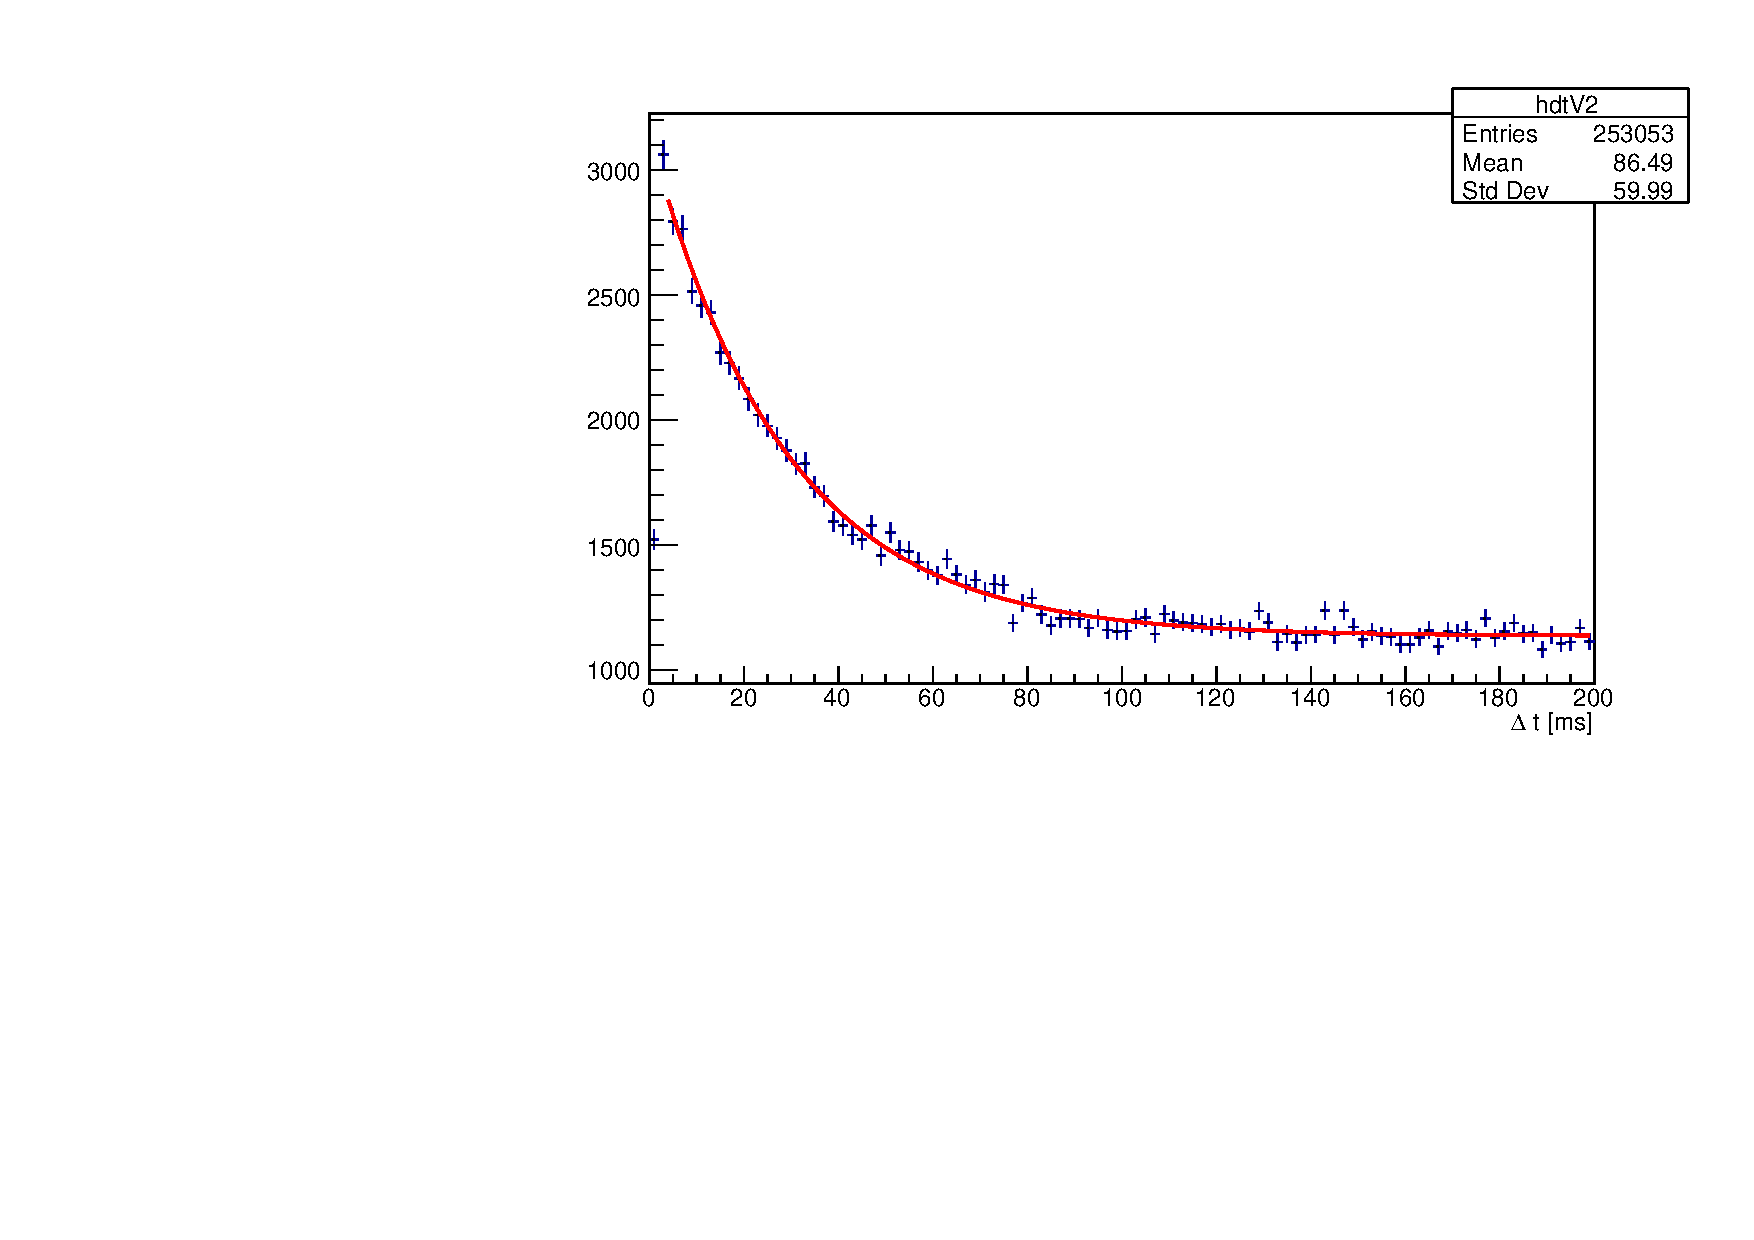
\includegraphics[width=60mm]{Figures/B12dt85.pdf}}\quad
\subfigure[The delay-prompt distance of $^{12}$B candidates]{\label{fig:distance}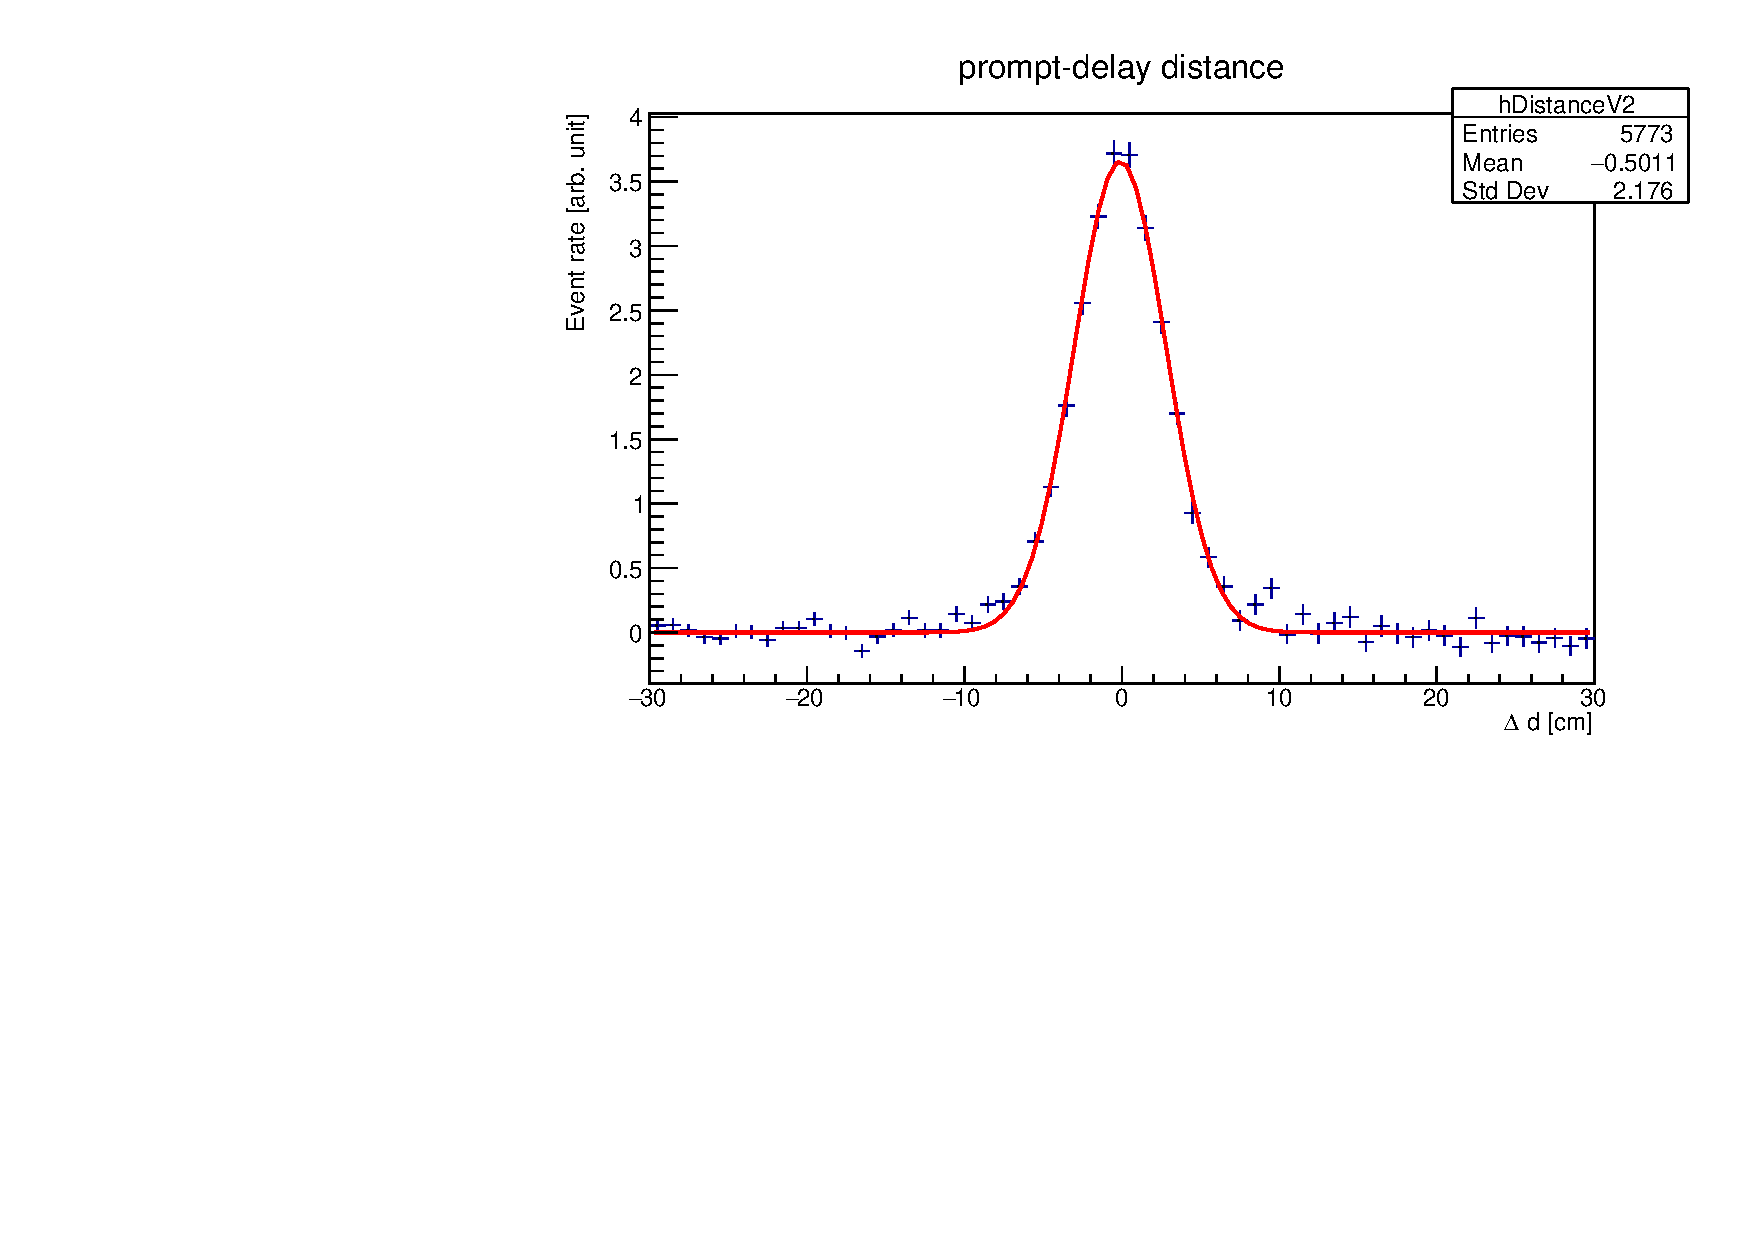
\includegraphics[width=60mm]{Figures/B12distance85.pdf}} \\
\subfigure[$^{12}$B spectrum.]{\label{fig:B12}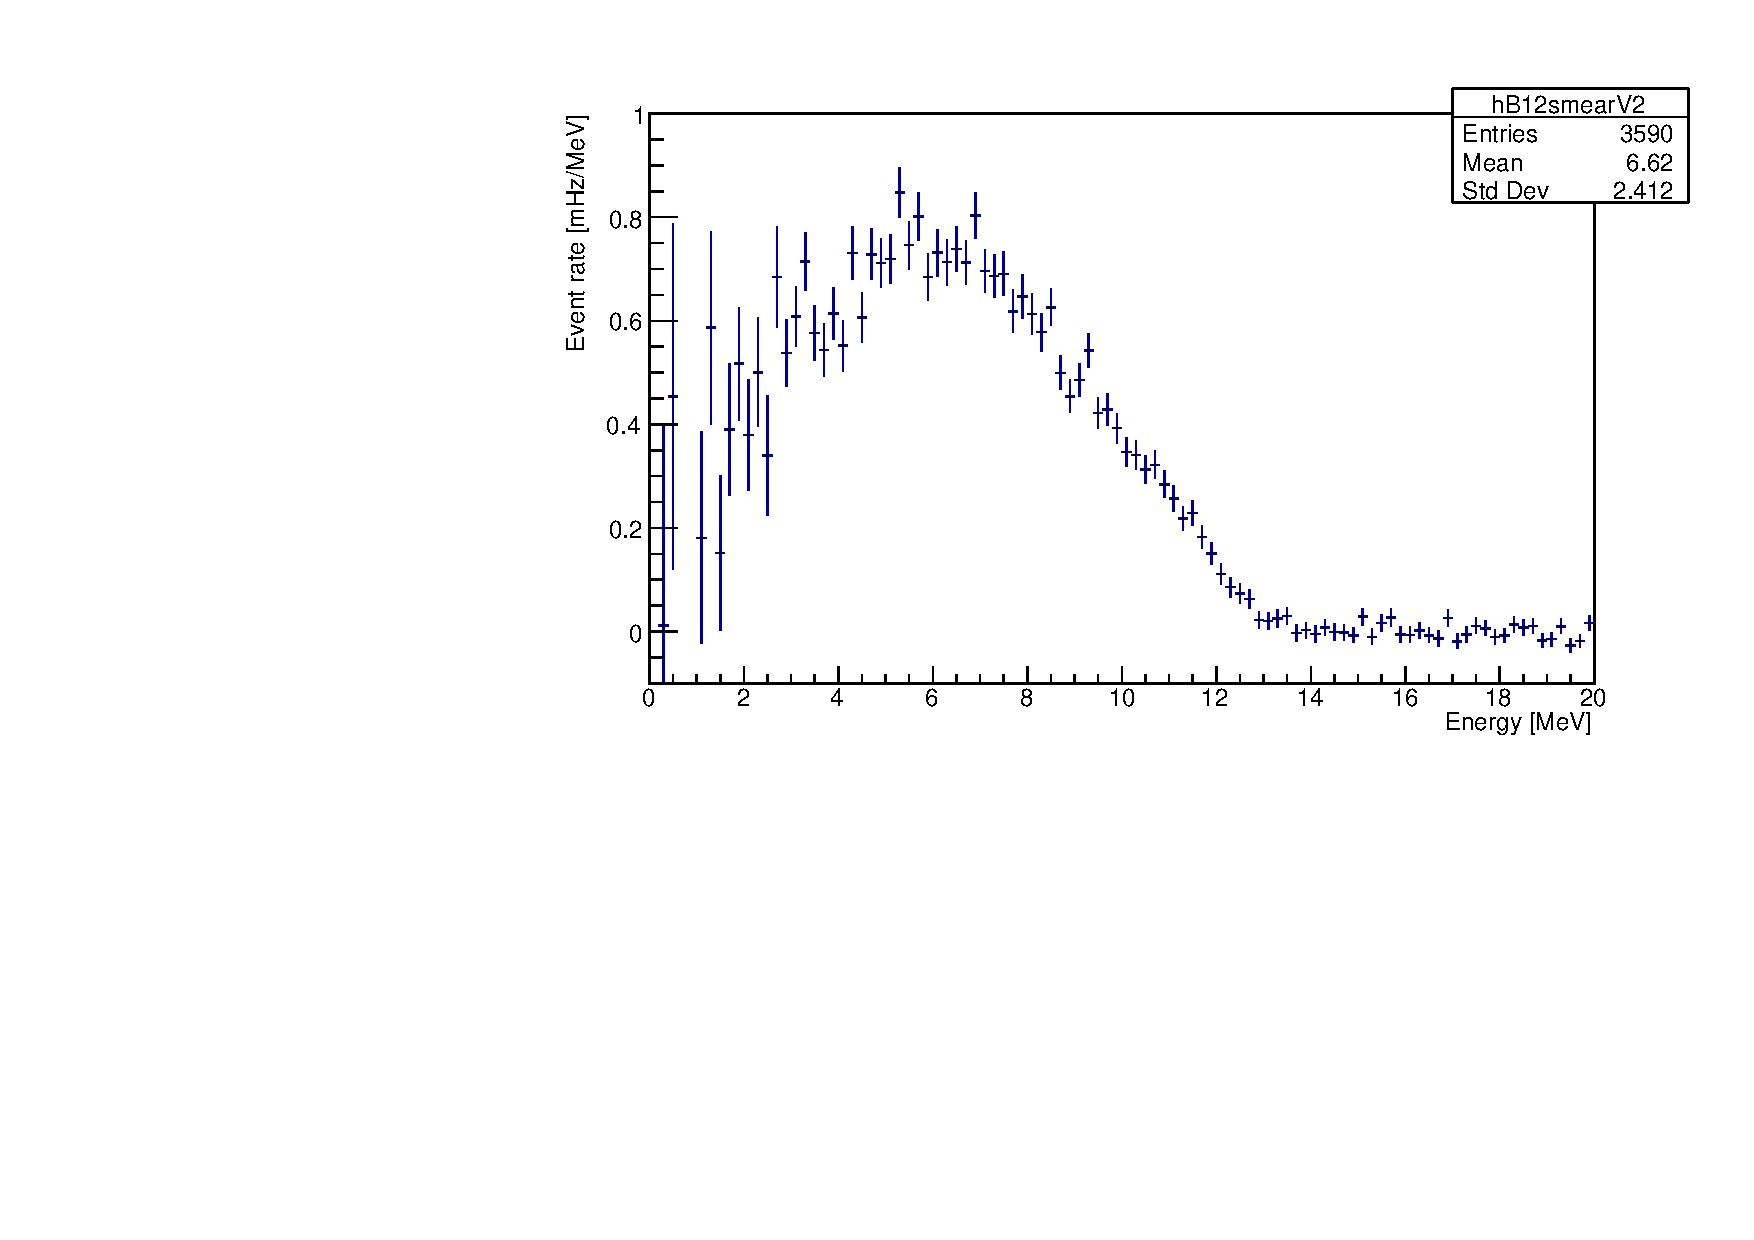
\includegraphics[width=60mm]{Figures/B12smear85.pdf}} 
\caption{The observation of $^{12}$B events in PROSPECT.}
\label{fig:B12plots}
\end{figure}

The AmBe calibration source is a composite neutron source, where the $\alpha$ emitted from $^{241}$Am interacts with $^9$B through
\begin{equation}
	\alpha + ^9\textrm{B} \rightarrow n + ^{12}\textrm{C} + 4.4 \textrm{MeV}
\end{equation} 
with a 4.4~MeV single gamma emission.
Although not used in the period in current neutrino data release, the 4.4~MeV gamma is a good cross check for PROSPECT to show its ability to reconstruct the higher energy gamma that covers the same energy range as the 4~MeV to 6~MeV IBD spectrum excess.
The single energy gamma is selected based on the time coincidence between the gamma-like prompt signal and the delayed $n$-Li capture signal using the discrimination with PSD.
A unique challenge in the event selection is that the neutron radiation of AmBe has 1~MeV scale kinetic energy, causing non-negligible mixing between gamma hit and proton recoil hit in the prompt event cluster.
The exclusion of proton recoil like hit from the prompt clusters managed to purify the prompt gamma events.
The energy spectrum of the AmBe gamma is shown in Figure~\ref{fig:AmBePlot}.
\begin{figure}[h!]
\centering
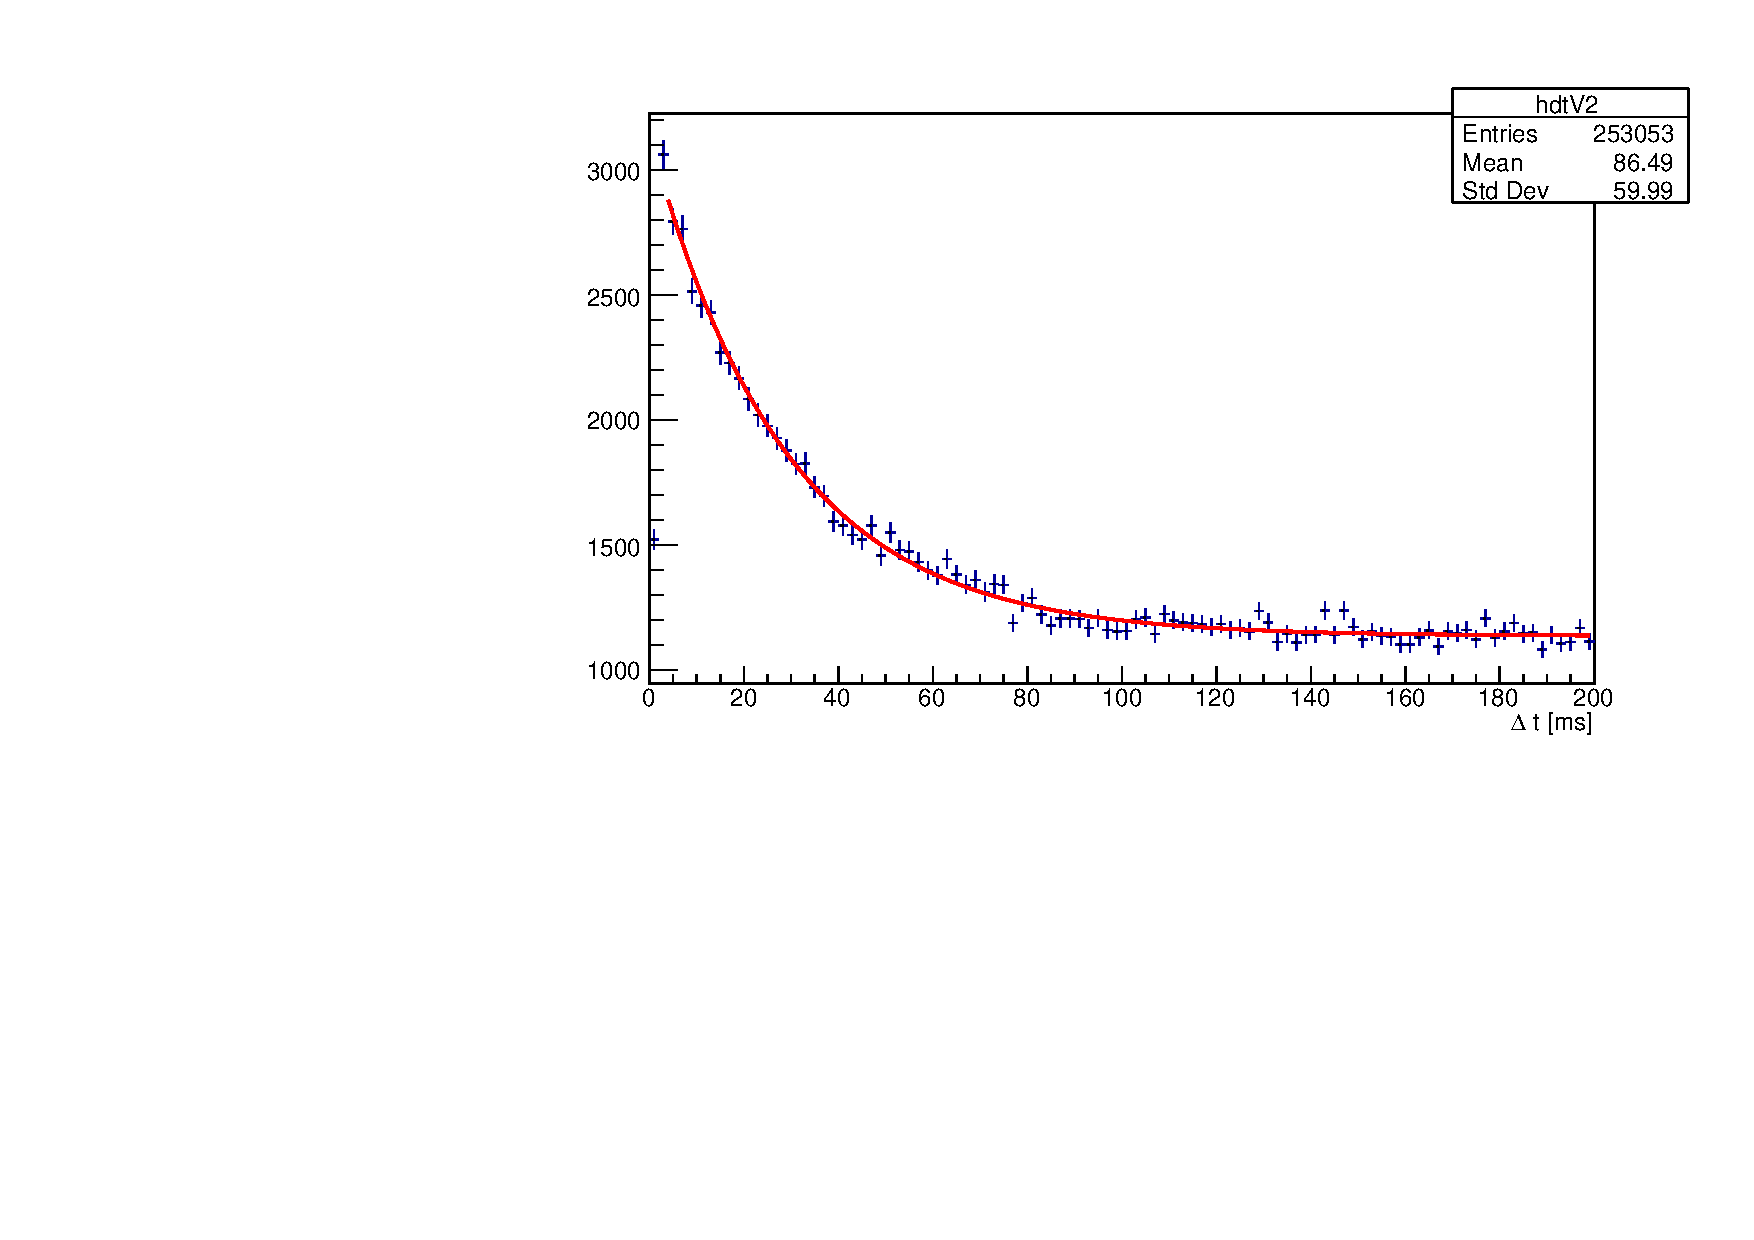
\includegraphics[width=0.45\textwidth]{Figures/B12dt85.pdf}
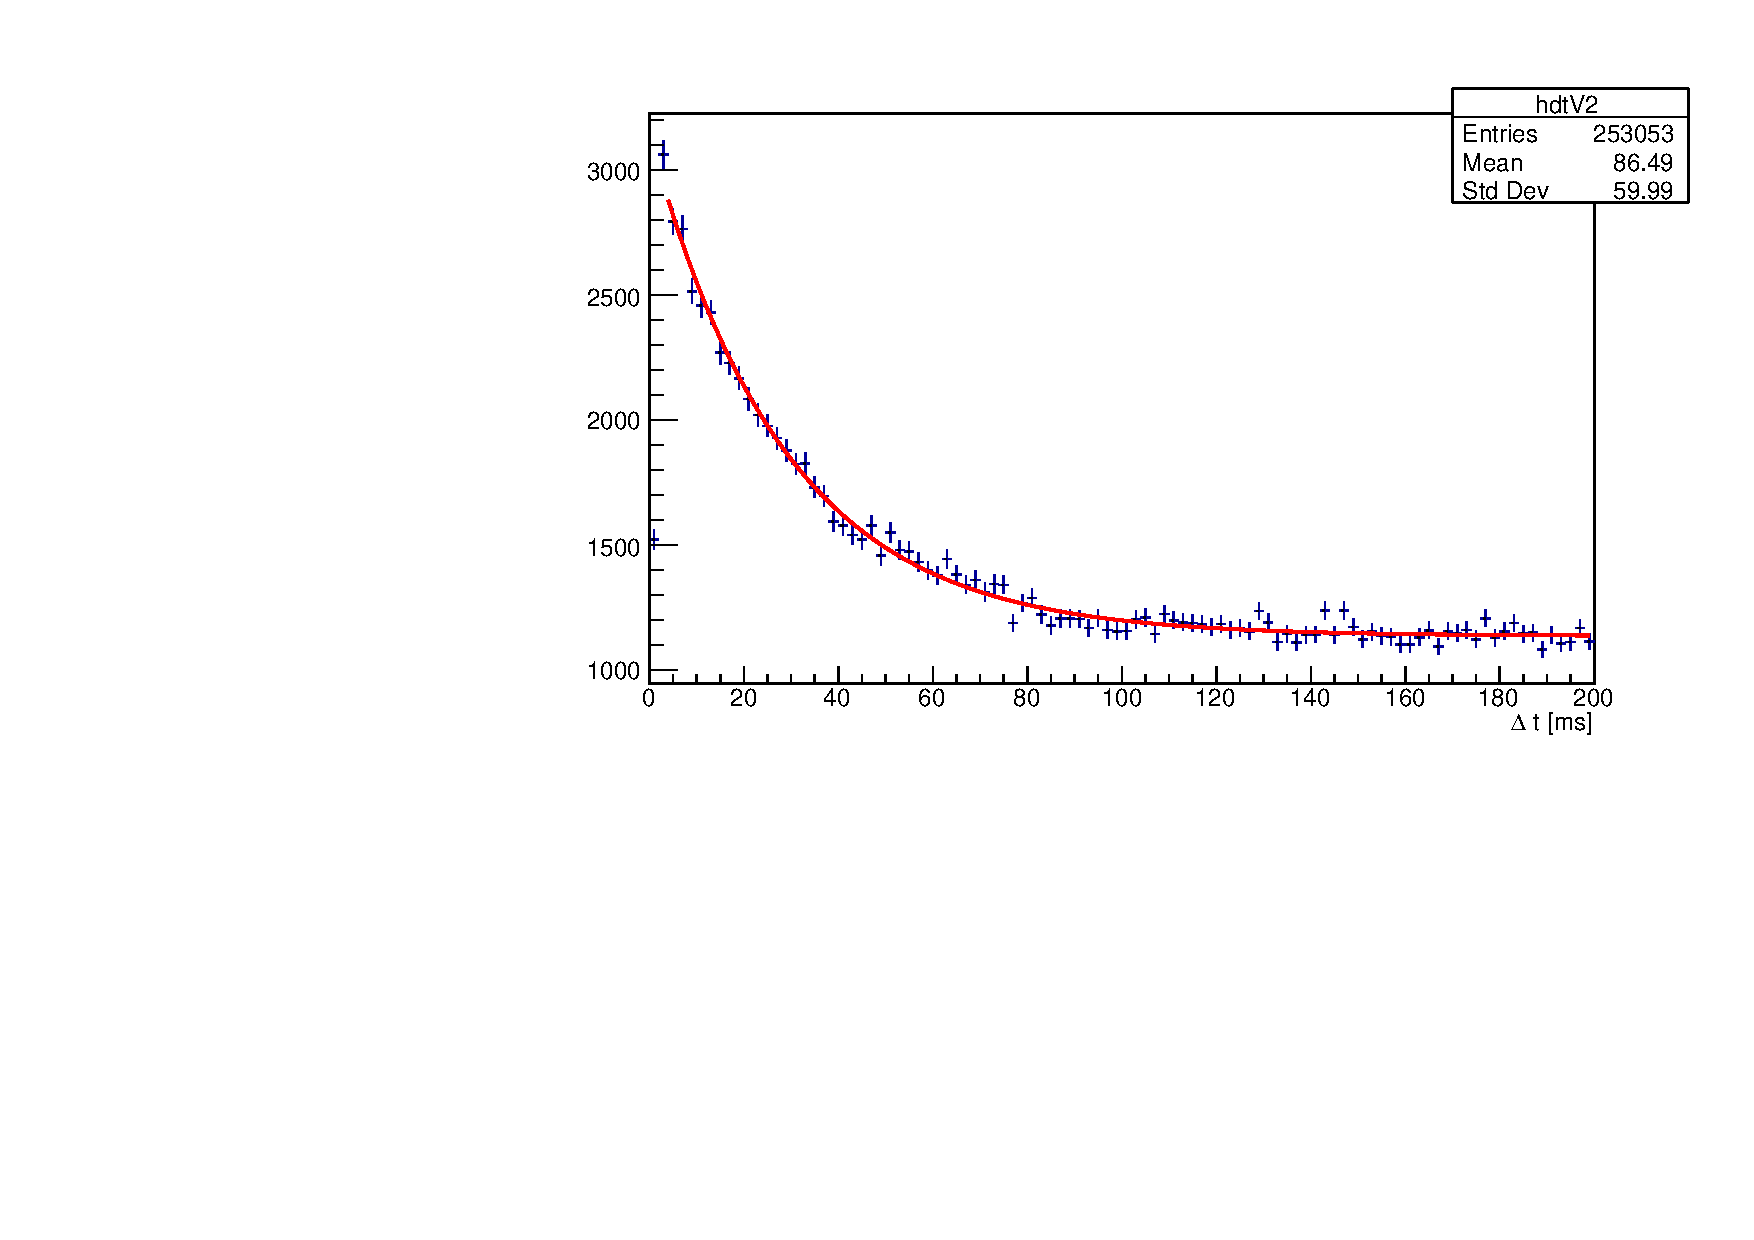
\includegraphics[width=0.45\textwidth]{Figures/B12dt85.pdf}
\caption[Reconstructed AmBe gamma energy]{The observation of $^{12}$B events in PROSPECT.}
\label{fig:AmBePlot}
\end{figure}

\newpage

\clearpage

\Section{Monte-Carlo Calibration Datasets}
The purpose of the comparison between MC and calibration data is to characterize the detector energy response, so we are able to make a trust worthy IBD prompt energy spectrum model to data comparison with precisely tweaked detector response model.
The detector response model also includes the LS's photoelectric effect and detector geometry influence. 
The Birks' quenching effect, the optical properties of PROSPECT AD components and the Cherenkov radiation induced by energetic particle can cause nonlinear energy reconstruction of incident event.
The detector dead volume made from the optical grid also affects the reconstructed energy with gamma escaping and energy loss.
In addition, there are relative energy scale affected by the difference among detector cells, caused by non-uniformity of LS and cell volume.
The resolution of the reconstructed energy are dominated by the time dependent photostatistics of LS and the geometry effects of detector, but the fluctation of energy resolution is eliminated by uniformly smearing the energy of every hits.
The artificial smearing was based on the worst energy resolution (lowest PE/MeV) calibrated during the production data and through ou the detector.
As a result, the first and second order Birk’s constant in detector $k_{B1}$ and $k_{B2}$, the detect efficiency of Cherenkov light $k_{C}$, and a absolute energy scale $A$ are the terms that were searched precisely. 
The MC reconstructed energy is  
\begin{equation}
E_{MC} = \sum_i A(E_{scint,i}(k_{B2},k_{B2})+E_{c,i}(k_C)),
\end{equation}
where $i$ is each GEANT4 step.
Later in this study, we will review the energy resolution as function of energy based on the best-fit detector response of the parameters listed above.

The PROSPECT-G4 simulation package was utilized to simulate all of the calibration with close-to-reality detector configurations as calibration data.
Other than the detector geometry and materials, the nonlinearity from Birks$^\prime$ quenching effect of scintillator and Cherenkov radiation induced by charged particles was simulated by PROSPECT-G4.

\Subsection{Nonlinearity}
\label{sec:nonlinear}
The energy response of LS is mainly affected by the Birks$^\prime$ law quenching and Cherenkov radiation. 

The Birks$^\prime$ law is a empirical function of the light yield per track length:
\begin{equation}
    \frac{dE_{scint}}{dx} = \frac{\frac{dE}{dx}}{1+k_{B1}\frac{dE}{dx}+k_{B2}(\frac{dE}{dx})^2},
\end{equation}
where $k_{B1}$ are $k_{B2}$ the Birks$^\prime$ constants relate to property of LS. 
They represent the quenched reconstructed energy in LS, a nonlinear energy loss caused by particle-molecule interaction. 
According to this function, $k_{B1}$ reduces the reconstructed energy of lower energy events, showed in Figure \ref{fig:kb1plot}.
Although $k_{B2}$'s effect is negligible in higher energy, it is capable to affect particle segment-hit multiplicity for its ability to quench more lower energy events below the 90 keV threshold, as shown in Figure \ref{fig:kb2plot}.
In MC, we  simulate the quenching effect by multiplying energy difference in between photoelectron steps with a Birk's factor:
\begin{equation}
   \frac{1}{1+k_{B1}\frac{dE}{dx}+k_{B2}(\frac{dE}{dx})^2}.
   \label{eql:birks}
\end{equation}

\begin{figure}[h!]
\centering
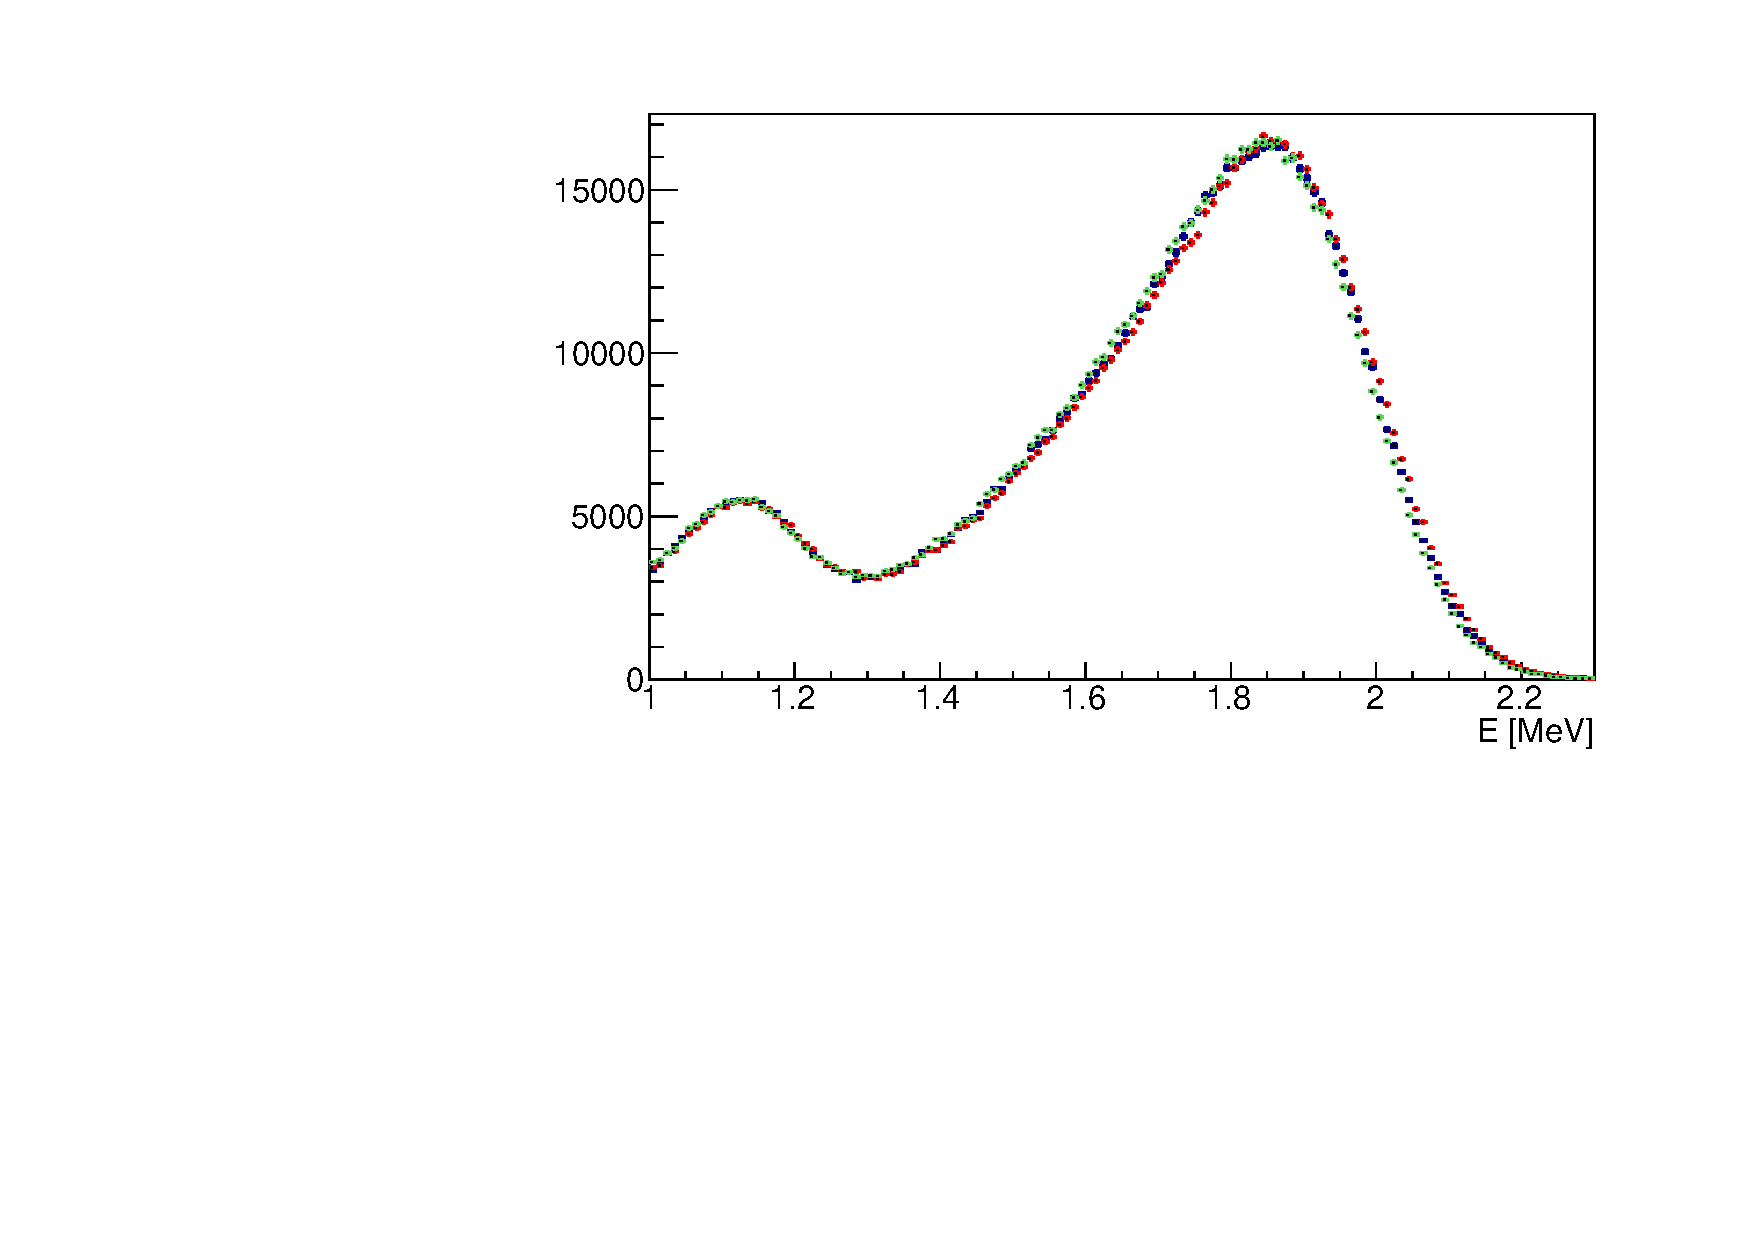
\includegraphics[width=60mm]{Figures/kb1.pdf}
\caption{The MC quenching induced by $k_{B1}$. (red: lower value, blue: norminal value, green: higher value)}
\label{fig:kb1plot}
\end{figure}
 
\begin{figure}[h!]
\centering
\subfigure[The energy distribution of $^{22}$Na simulation affected by $k_{B2}$.]{\label{fig:kb2}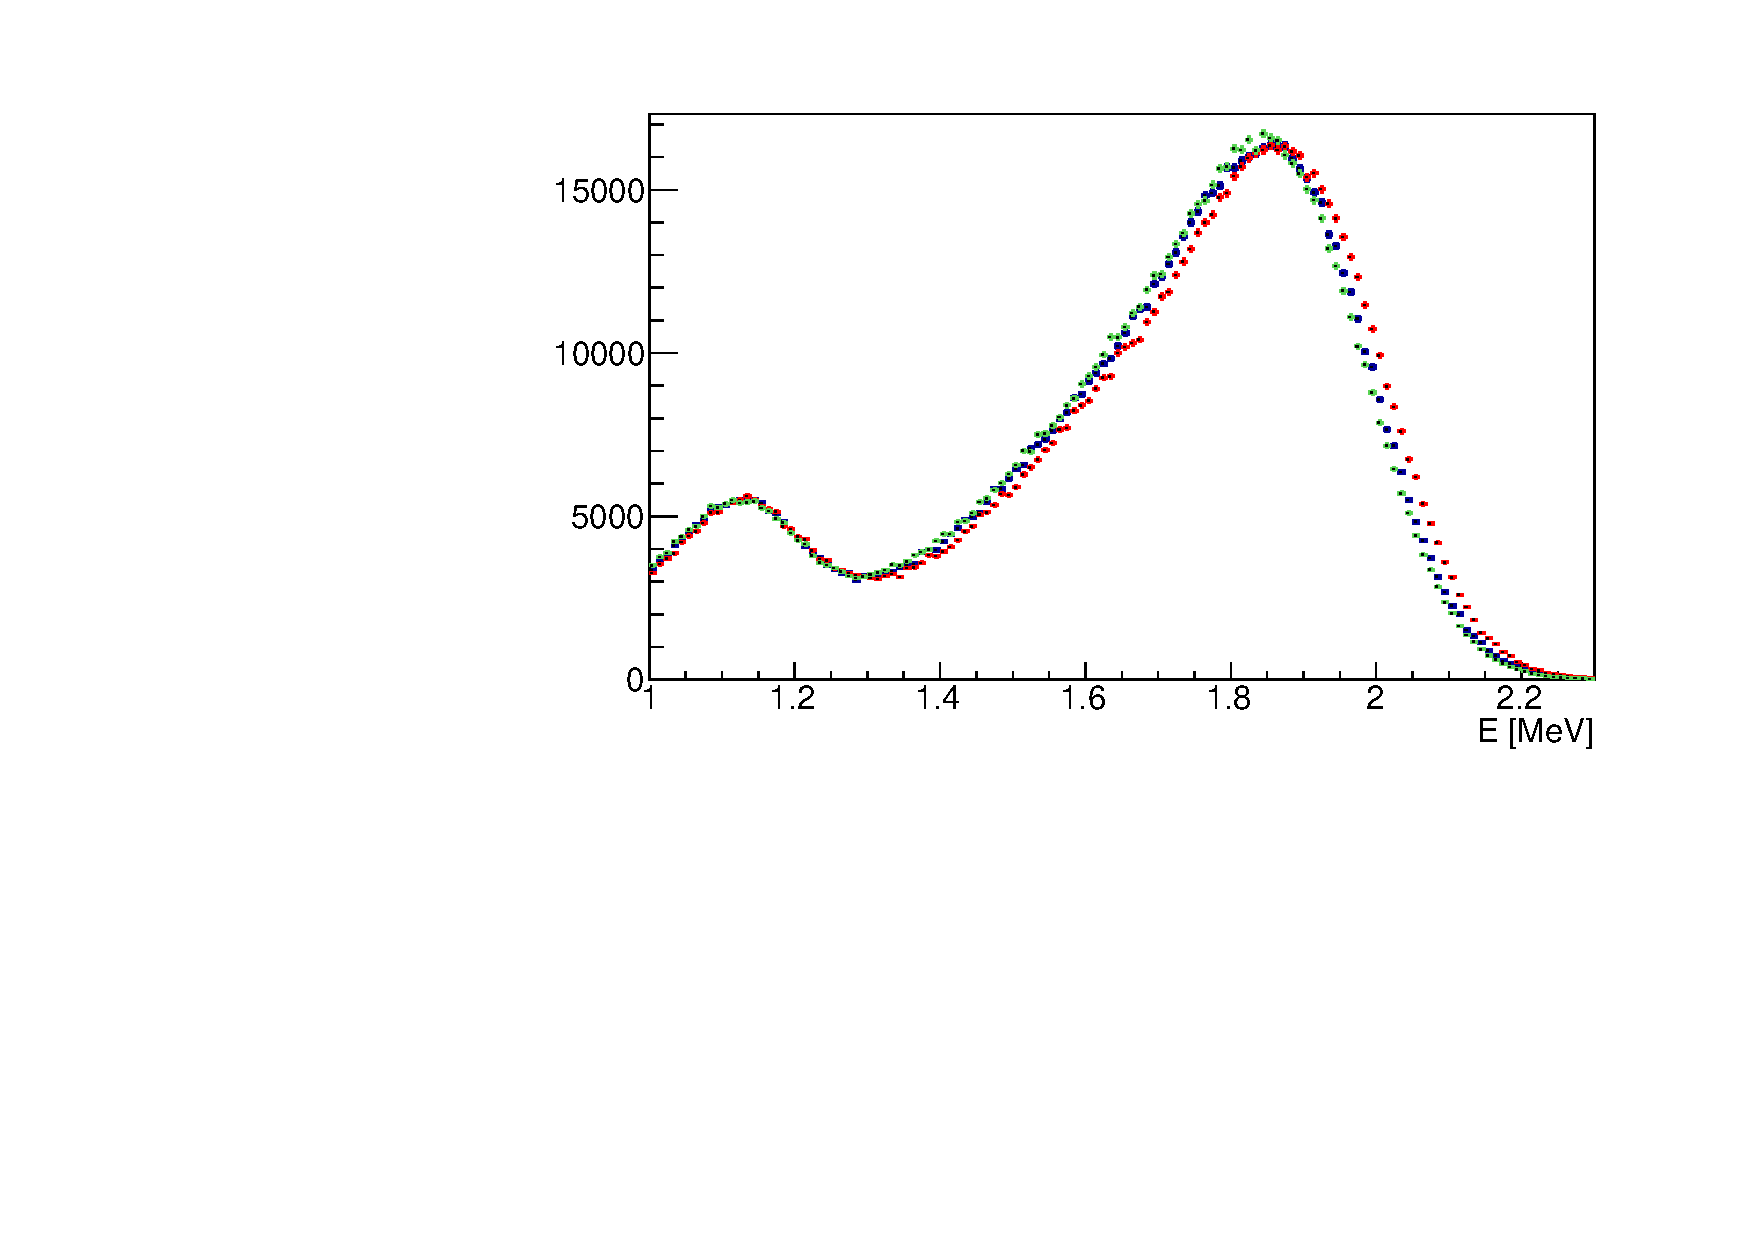
\includegraphics[width=60mm]{Figures/kb2.pdf}}\quad
\subfigure[The $^{22}$Na cell-hit multiplicity affected by $k_{B2}$. ]{\label{fig:kb2multi}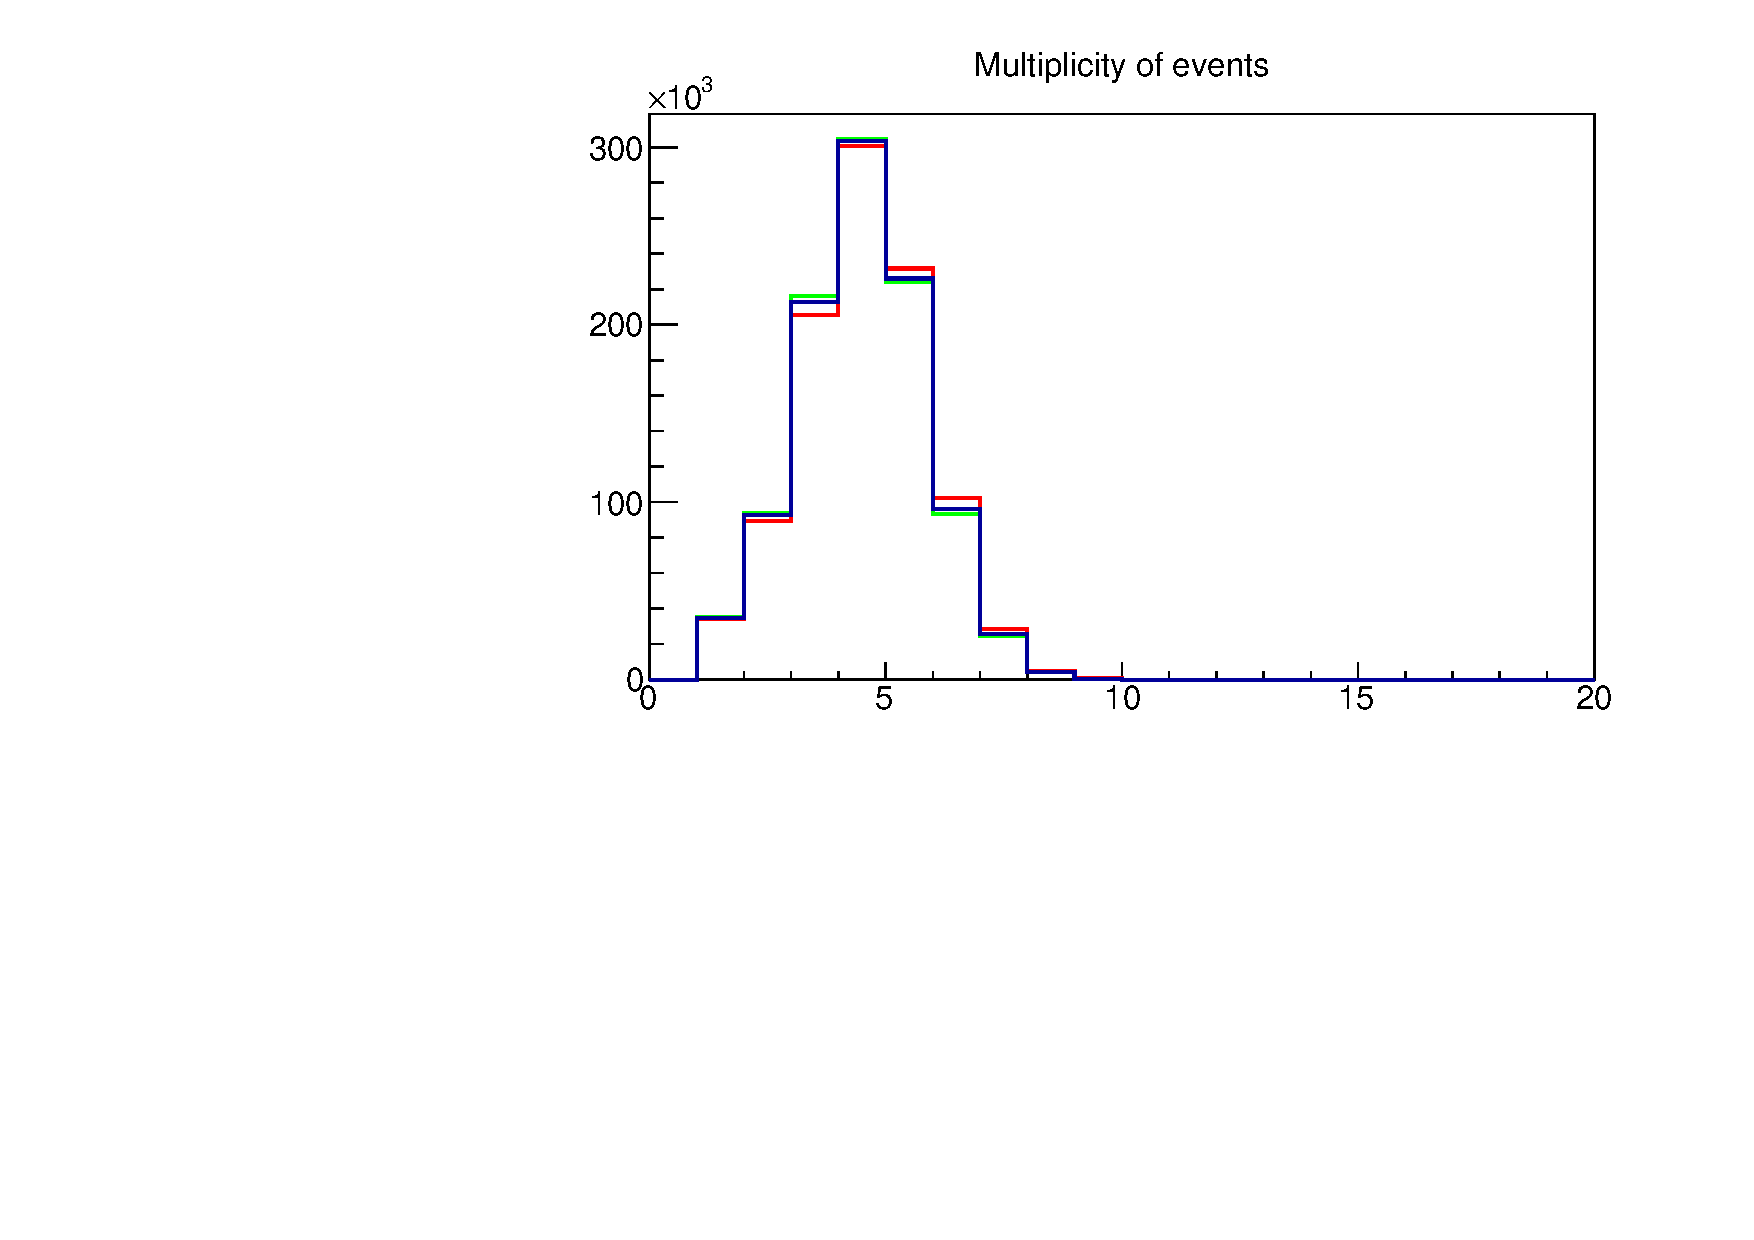
\includegraphics[width=60mm]{Figures/kb2multi.pdf}}
\caption{The MC quenching induced by $k_{B2}$. (red: lower value, blue: norminal value, green: higher value)}
\label{fig:kb2plot}
\end{figure}

The Cherenkov radiation is the light emitted as a charged particle traveling faster than the phase velocity of light in a medium. 
The molecules in the medium are polarized along the particle track, when the particle is faster than light, the electromagnetic field of molecule depolarization can add up as coherent light emission. 
The number of photon generated along the particle track can be expressed as:
\begin{equation}
    \frac{d^2N}{dxd\lambda} = \frac{2\pi\alpha z^2}{\lambda}\left(1- \frac{1}{\beta^2n^2(\lambda)}\right),
\end{equation}
where $N$ is number of photon, $\alpha$ is a fine structure constant, $z$ is the particle's electric charge, $\beta$ is the speed of the particle and $n(\lambda)$ is index of refraction.
Although most of Cherenkov light is in UV range, the LS is able to absorb and re-emit it in VIS range with currently unknown efficiency.
Therefore, more light can be collected in addition to the scintillation light with high energy incident charged particle and increase reconstructed energy, when particle is kinetic energy is high enough to exceed the phase velocity of light.
In MC processing, we collected the energy emitted from the Cherenkov radiation as the summed energy of detected Cherenkov photons,
\begin{equation}\label{eq:ceren2}
E_{c} = k_{c}\sum_{\lambda}N_\lambda E_\lambda,
\end{equation}
where the uniform of Cherenkov optical spectrum is assumed.
The LS's index of refraction and detect efficiency is also assumed a constant against wavelengths in 200-700 nm range.
Then we use the the detect efficiency of Cherenkov light, $k_{C}$, in percentage, to model the effect of Cherenkov radiation on reconstructed energy. 
The particle energy loss in Cherenkov radiation is negligible.
Figure \ref{fig:kcplot} showed different $k_{C}$ values affecting the n-H capture spectrum.

\begin{figure}[h!]
\centering
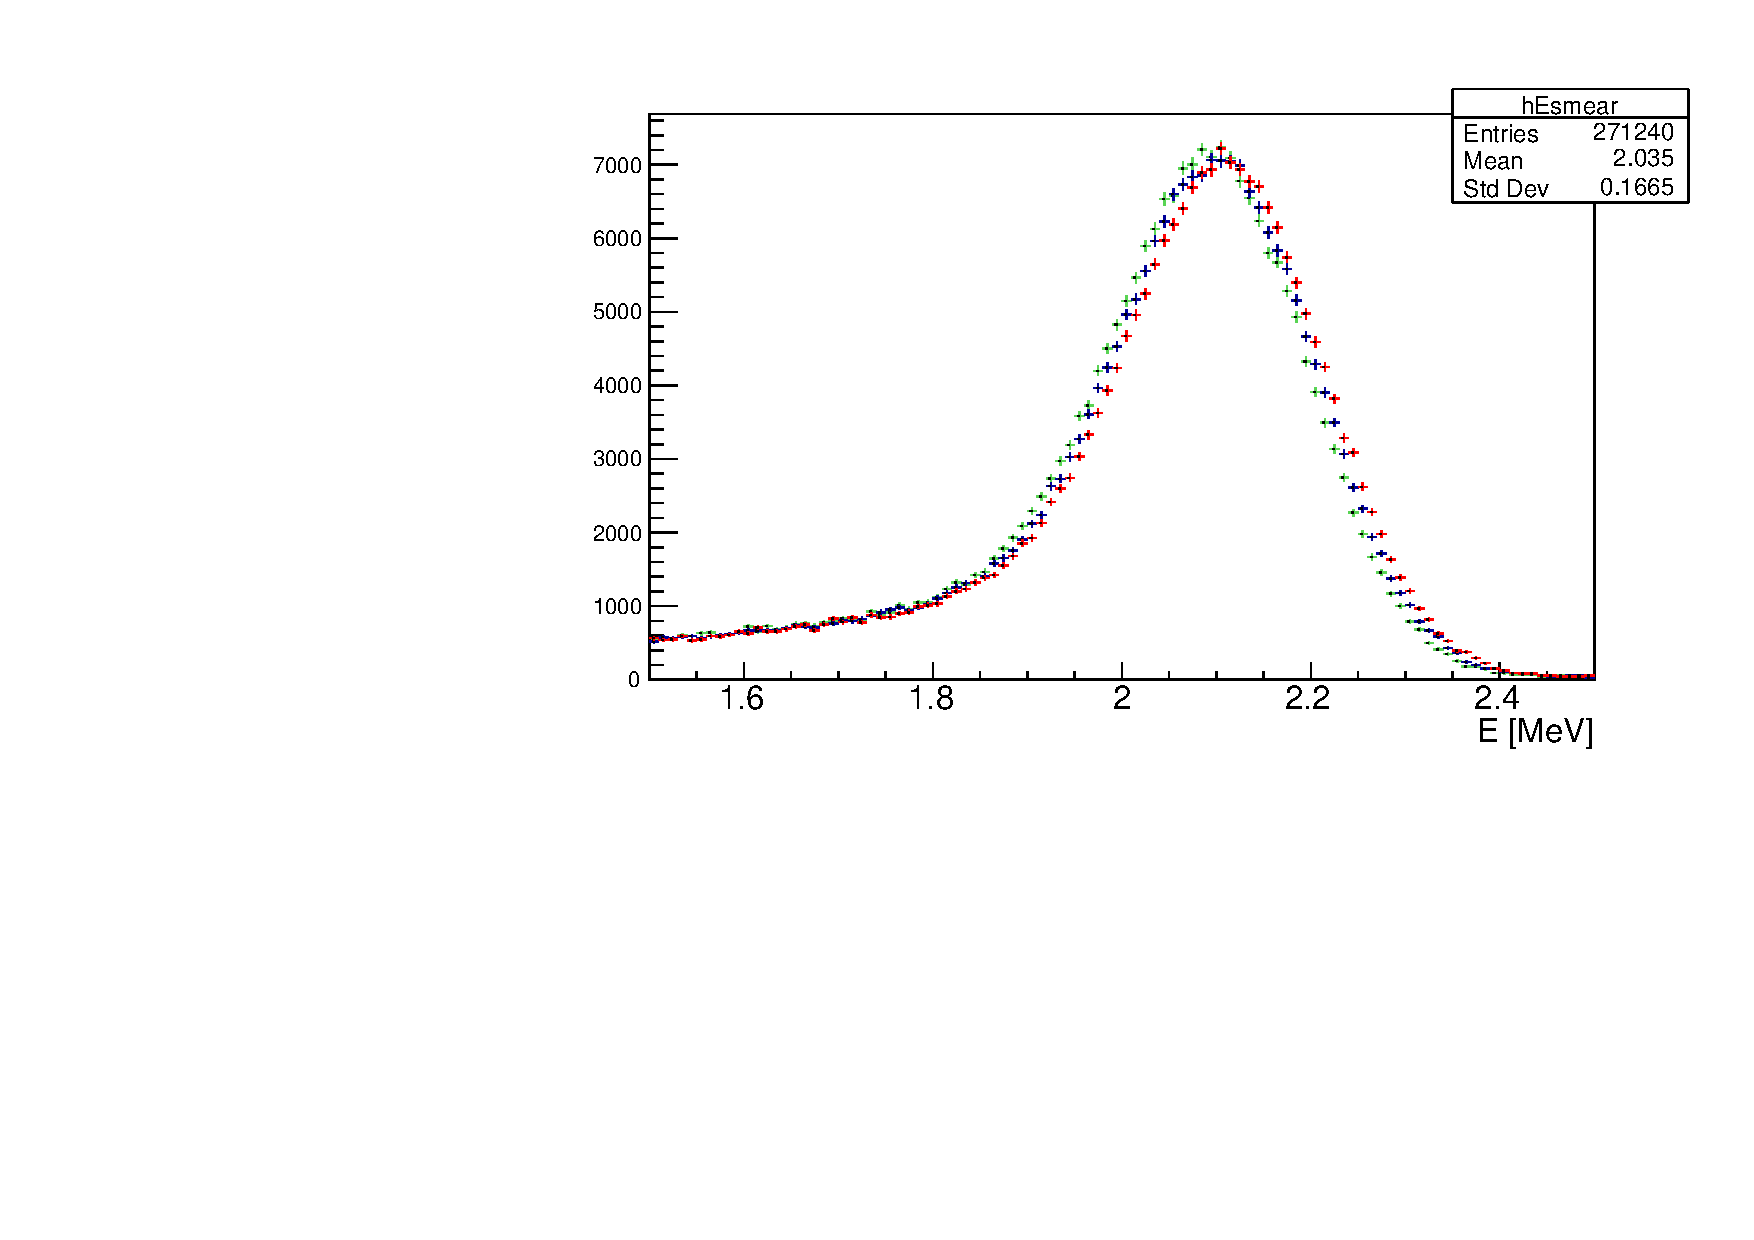
\includegraphics[width=60mm]{Figures/kc.pdf}
\caption{The MC Cherenkov radiation effect induced by $k_{C}$. (green: lower $k_{C}$, blue: norminal $k_{C}$, red: higher $k_{C}$)}
\label{fig:kcplot}
\end{figure}

To simply model the detector energy response, the Birks$^\prime$ constants $k_{B1}$ and $k_{B2}$ in equation \ref{eql:birks} and the detect efficiency of Cherenkov light $k_C$ were adjusted freely to search the best-fit nonlinearity model with data. 
The parameter search was in the range $(0.100, 0.136)$ mm/MeV for $k_{B1}$ with 0.004 mm/MeV steps, $(0.003, 0.039)$ mm/MeV for $k_{B2}$ with 0.004 mm/MeV steps and $(30, 50)\%$ for $k_C$ with $2\%$ steps. 
We performed calibration simulations for each group of the $k_B$s and $k_C$ combination and scanned through 1000 models .
The simulation involving optical photon is computationally expensive regarding to the scale of MC processed, we applied the nonlinearity corrections only to the energy o each GEANT4 steps.

\Subsection{Energy Resolution}
\label{sec:resolution}
The reconstructed resolution is a function of energy:
\begin{equation}
\label{eql:resolution}
    \frac{\sigma}{E} = \sqrt{a^2 + \frac{b^2}{E}+\frac{c^2}{E^2}},
\end{equation}
where $a$ is affected by the detector geometry, $b$ is from the photostatistics (PE/MeV) and $c$ for the quantum efficiency of PMTs.

%To reduce the computer resource required for the fitter, we neglected $a$ and $c$ of the resolution function, then used MINUIT $\chi^2$ minization to find the best $b$ value, while allow $b$ change freely.

\Subsection{Other Energy Scale Factors}
\label{sec:other}
The reconstructed energy scale was initially based on the assumption that $n$ captured by $^6$Li yield 0.55 MeVee in detector. 
The deviation of true electron equivalent energy to this estimation can induce a constant energy scale throughout the all energy. 
This absolute energy scale $\beta_{rec}$, as a fitting parameter, was searched together with other energy response parameters.
Similar to the resolution term $b$, we allowed MINUIT minization of $\chi^2$ to freely change $\beta_{rec}$ until we found the minimum the $\chi^2$ between data and MC.

%The zero length encoding (ZLE) threshold was applied during data acquisition, requiring each ADC channel to record signals that are only above specific magnitude. 
%By excluding electronic noise, this threshold also affect the energy scale nonlinearly by excluding small deposition of energy in some segments in multi-hit events. 
To ensure MC being precisely compared to data, ZLE threshold was simulated in CalcDetectorPulseResponse program by convert energy deposit in MC to pulse with respect to ADC/PE ratio.
The 85 keV energy threshold was then applied to the calibration MC using same P2x analysis plugin.
%However, although quenching and detector effects were simulated in MC, the event selection based on the unsmeared energy of each hits (it is computationally expensive to smear simulation energy before energy cut, because it requires reanalyze MC everytime when each new resolution candidate is thrown).
%This reversed processing will result in MC keeping more low energy hits than data, then causing miss match between data and MC because of different cell-multiplicity per event.
%Thus a higher energy threshold whose smeared lower edge is close to the 85 keV is compromising.
%To resolve the issue with reversed data processing, an alternative energy threshold was searched from 65 to 90 keV with 5 keV steps.

\Subsection{Detector Geometry Simulation}
The difference between simulated detector and the built detector could lead to disagreement in energy loss and gamma leakage between MC and data. 
The reconstructed energy of multi-cell-hit particle is affected by the separator thickness, pinwheel rod size and all materials that the particle can possibly travel through. 
In this work, we surveyed the thickness and material of the separator, the pinwheel rod dimensions and thickness, the inner structure inside pinwheel rods, the density and mixture of LS and calibration capsule properties, based on detector design and QA measurements.
Out of those detector properties, the thickness of separators play non-negligible roles in eventenergy loss. 
The thickness and uncertainty of the separator is $1.18 \pm 0.05$ mm, which is described in reference "DOCTHICK".

\begin{figure}[h!]
\centering
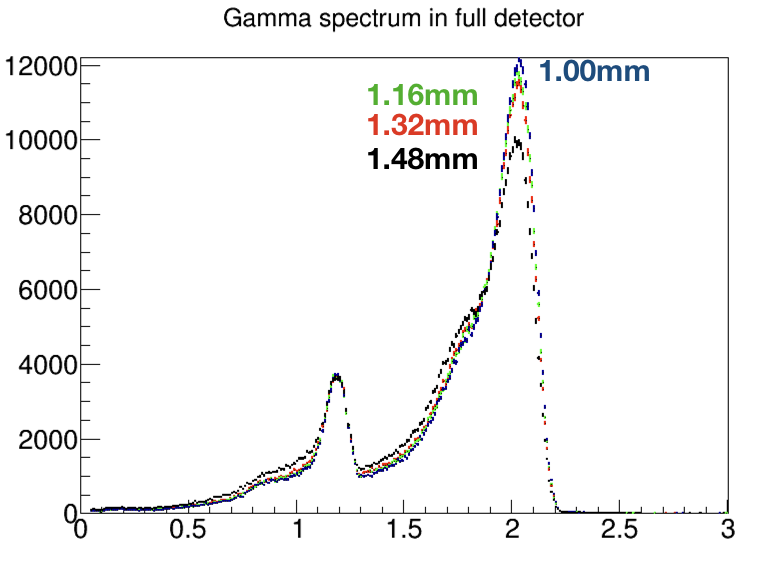
\includegraphics[width=80mm]{Figures/thickness.png}
\caption{The example showing the thickness of separators affecting the energy loss and so the spectrum.}
\label{fig:thickness}
\end{figure}

Besides, we found the uncertainties of the dimensions of the other inner detector materials played negligible role in energy loss. 
For instance, the variation thickness of the pinwheel rode, which carries the similar uncertainty as separators, did not change the reconstructed energy visibly, even with exaggerated $0.25$ mm uncertainty showed in Figure \ref{fig:pinwheelthick}.

\begin{figure}[h!]
\centering
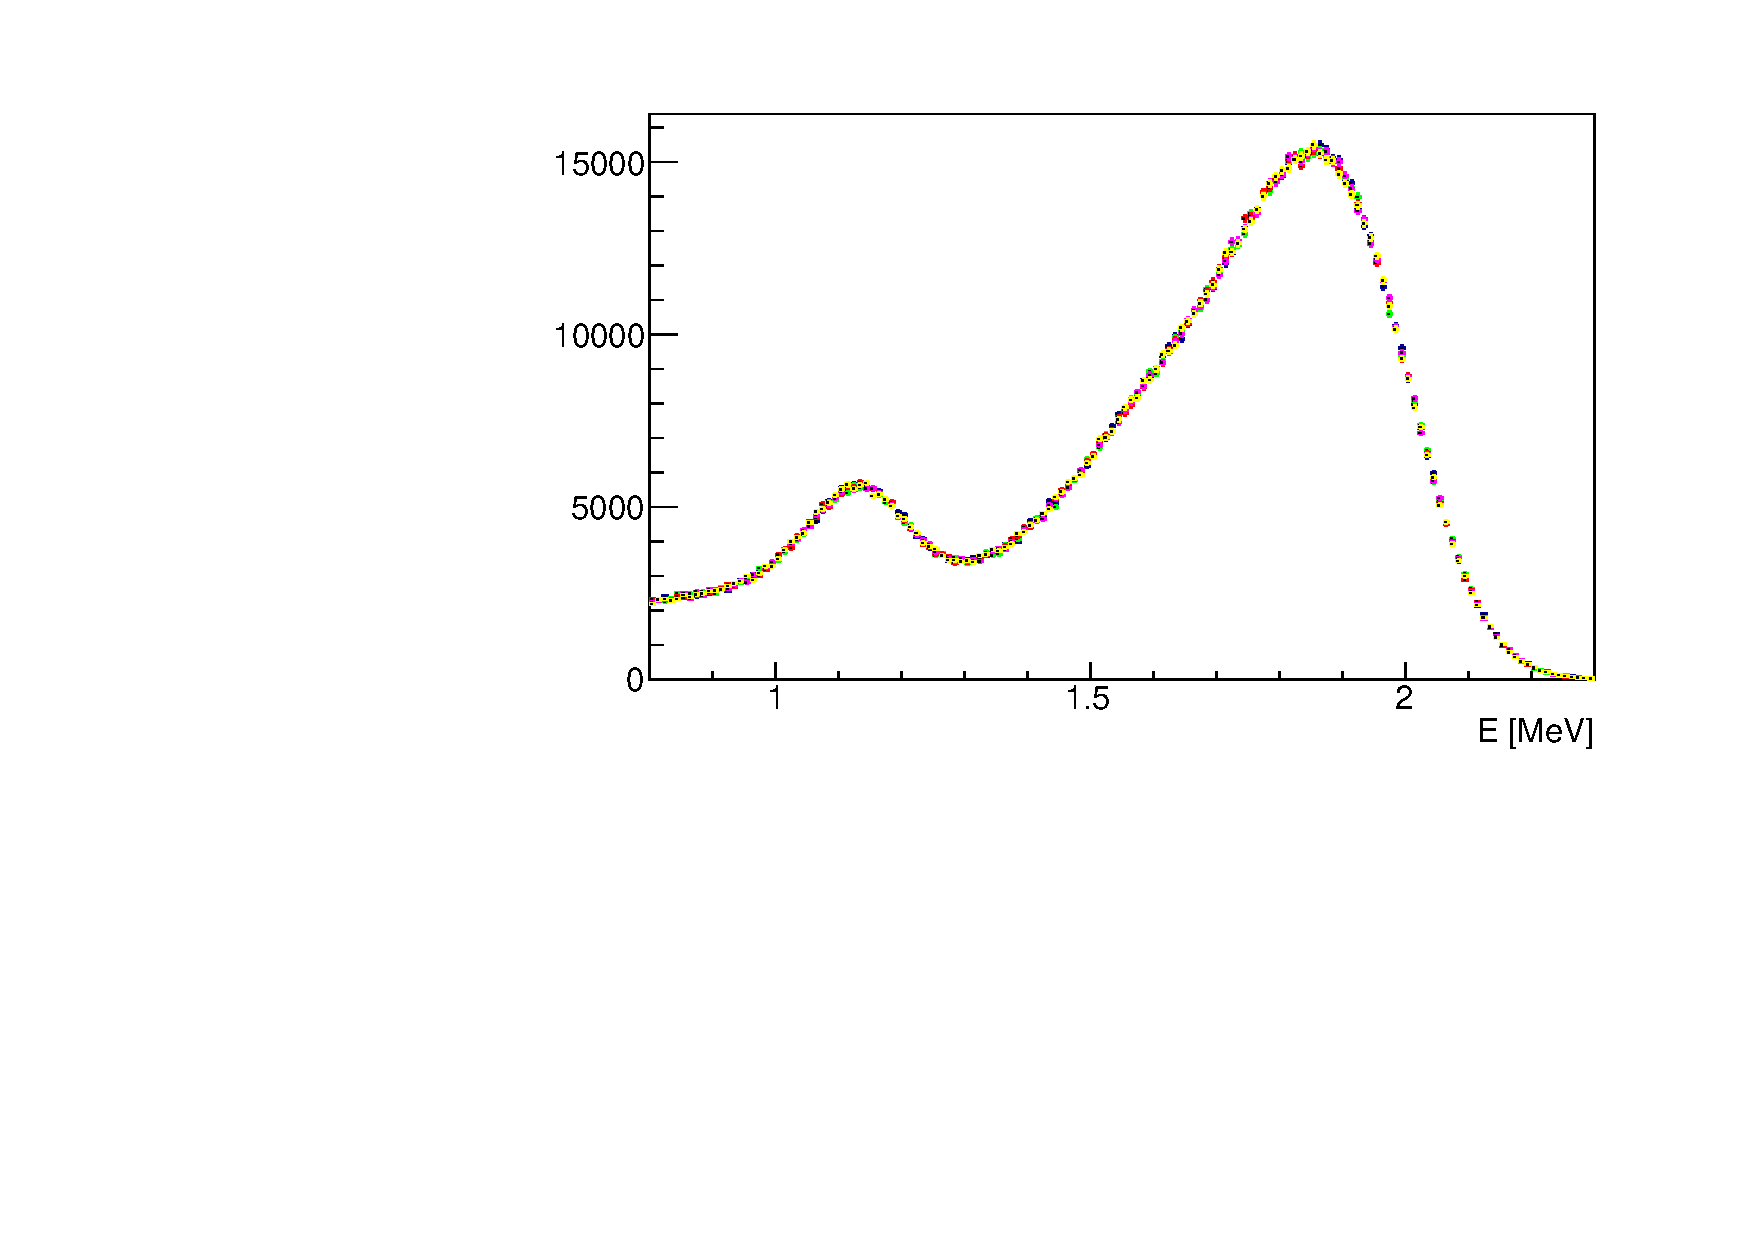
\includegraphics[width=80mm]{Figures/pinwheelthick.pdf}
\caption{The example showing the thickness of piwheel rods$^\prime$ ignorable effect on the energy loss. (blue: 12.1 mm; red: 12.2 mm; green: 12.3 mm; pink: 12.4 mm; yellow: 12.5 mm)}
\label{fig:pinwheelthick}
\end{figure}

\Subsection{Calibration Input Model}
The input model of radioactive calibrations was based on the decay branching from ENSDF database.
We simulated 1 million decays individually for each nonlinearity model scanned and each of the radioactive calibrations, which is comparible to the real event rates.
The decay branching fraction and energy scale in the simulation input are negligible.
The decay branches of $^{12}$B is based on reference \cite{bib:duke}. 
We generated 250,000 $^{12}$B decays in simulation, which is considerably more stastics than data collected.
During data vs MC comparison, the $\sim$1\% energy scale uncertainty of $^{12}$B input spectrum was taken into consideration by pulling the energy scale of $^{12}$B spectrum in 1\%. 
The uncertainty in $^{12}$B decay branching fractions are negligible.

\Section{Data vs Monte-Carlo Comparison}
\label{sec:dataMC}
The MC calibration spectra and gamma multiplicities were compared with data through $\chi^2$ test. 
We generated a list of calibration MC with a variety of $k_{B1}$, $k_{B2}$ and $k_C$ as mensioned in section \ref{sec:nonlinear}. 
The MC files were converted to pulses and processed through similar analyzing loop as calibration data, including the energy-pulse conversion, the event based smearing and the ZLE thresholds.
The data vs. MC comparison was made with similar detector configuration, including same dead channels, comparable event rate and same size of fiducial volumes.
Then the analyzed MC spectra were scaled with a constant energy scale $A$, while both data and MC were artificially smeared with the energy resolution as described in section \ref{sec:resolution}.
Each $\chi^2$ is evaluated considering the statistical uncertainties of both MC and data, which is defined as 
\begin{equation}
	\chi^2 = \sum_i\frac{(O_i - WE_i)^2}{\sigma_O^2 + W^2\sigma_E^2},
\end{equation}
where $O$ and $E$ represent data and MC respectively, $W$ is the normalization factor of MC spectrum or multiplicity, and $\sigma_O$ and $\sigma_E$ are statistical uncertainty of data and MC.
To find the best fit detector response model, the combined $\chi^2$ value is defined as
\begin{equation}\label{eq:escalechi2}
    \chi^2_{data-MC} = \sum_{\gamma} \chi^2_\gamma + \sum_{multi}\chi^2_{multi} + \chi^2_{^{12}\textrm{B}},
\end{equation}
where $\sum_{\gamma} \chi^2_\gamma$ is summed $\chi^2$ of gamma energy spectrum, $\sum_{multi} \chi^2_{multi}$ is summed $\chi^2$ of gamma multiplicity, and $\chi^2_{^{12}\textrm{B}}$ is calculated by data-MC comparison of the $^{12}$B beta spectrum.
The MINUIT $\chi^2_{data-MC}$ minimization method was utilized to find the best fit four parameters. 

We performed the $\chi^2$ minimization on data-MC comparison of full-detector reconstructed energy spectra and gamma multiplicity.
The best-fit model was then cross-checked with the measured the detector segments that are most adjacent to the calibration sources, which is mainly affected by the LS light yield.

\Subsection{Full Detector Spectrum Comparison}
\label{sec:fulldet}
The full detector reconstructed energy spectrum is the distribution of the summed energy of every hit within an event cluster. 
Each cluster is a group of hits collected by adjacent individual LS cells and the gap between each hit being less than 20 ns.
The detector nonlinearity affected the full detector energy spectrum not only through energy scale, but also through cell-hit multiplicity, for different quenching coefficient can reserve or reject hits through the 85 keV threshold of single cell measured energy.
Therefore, in our searching of the best-fit nonlinearity model, we aimed to minimized the $\chi^2$ of a combined data-MC energy spectrum and hit multilicity comparison. 
In detail, the data-MC comparisons of the energy spectrum of gamma calibrations, the n-H capture gamma from $^{252}$Cf and $\beta$-decay of $^{12}$B were done simultaneously.
Considering the precision of event source location, we performed multiplicity comparison only on the gamma calibrations, containing $^{22}$Na, $^{137}$Cs and $^{60}$Co.

%As discussed in section \ref{sec:single}, the full detector reconstructed energy was not only quenched by LS, but also affected by energy loss and particle leakeage caused by inner materials of detector.
%Besides, the energy threshold in each cell contributed to the energy loss indirectly by affecting the cell-multiplicity of events.
%Ideally, the full detector's quenching model is same as single cell and PG4 package is able to simulate these energy loss and thresholding effects. 
%However, currently the best fit parameters from full detector data vs MC comparison shows poor agreement with single-cell best fit.
%The most likely reason is an unresolved nonlinearity based on detector cell-multiplicity of the incident event, which is currently under investigation, but do not effect overall energy scale significantly.
%Given this context, we chose to examine two methods related to full-detector energy scales: applying BF single-cell parameters to full-detector data/MC comparison, and separately performing a minimization on the full-detector data/MC comparison.

%As mentioned in Section \ref{sec:other}, we scanned through a variety of threshold and found 85 keV threshold is able to effectively reproduce the cell-multiplicity events from data, whose lower energy bound after smearing converted to $\sim73$ keV by assuming energy resolution as $4.2\%/\sqrt{E}$.

In full detector data vs. MC comparison, for the radioactive source calibrations, we tagged the peaks of the energy spectrum and picked the $3-\sigma$ region around the peaks as range of fitting. 
For $^{12}$B comparison, we chose 3 to 13.5 MeV as energy range of interest.

The figure \ref{fig:goodfit2} shows the full detector calibration spectra comparison best-fit model, where $\chi^2/NDF = 807.847/331$ with the parameters: $k_{B1} = 0.122 \pm 0.002$ mm/MeV, $k_{B2} = 0.023 \pm 0.002$ mm/MeV $k_C = 41 \pm 1\%$, with absolute energy scale of $\beta_{rec} = 100.36\pm0.2\%$. 
There was $\chi^2/NDF = 205.9/60$ contributed by the multiplicity fitting.
In the energy spectra comparison, the biggest contributor of the disagreement is n-H capture gamma with $\chi^2/NDF = 175/40$.
The data-MC energy spectra comparison of the best-fit model is shown in Figure \ref{fig:goodfit2}, and multiplicity comparison is shonw in Figure \ref{fig:multi}.
The $\chi^2$ distributions depent on $k_{B1}$ and $k_{B2}$, and $k_{B1}$ and $k_{C}$ are shown in Figure \ref{fig:chi2}.

\begin{figure}[h!]
\centering
\subfigure[Full detector MC-data for $^{137}$Cs calibration.]{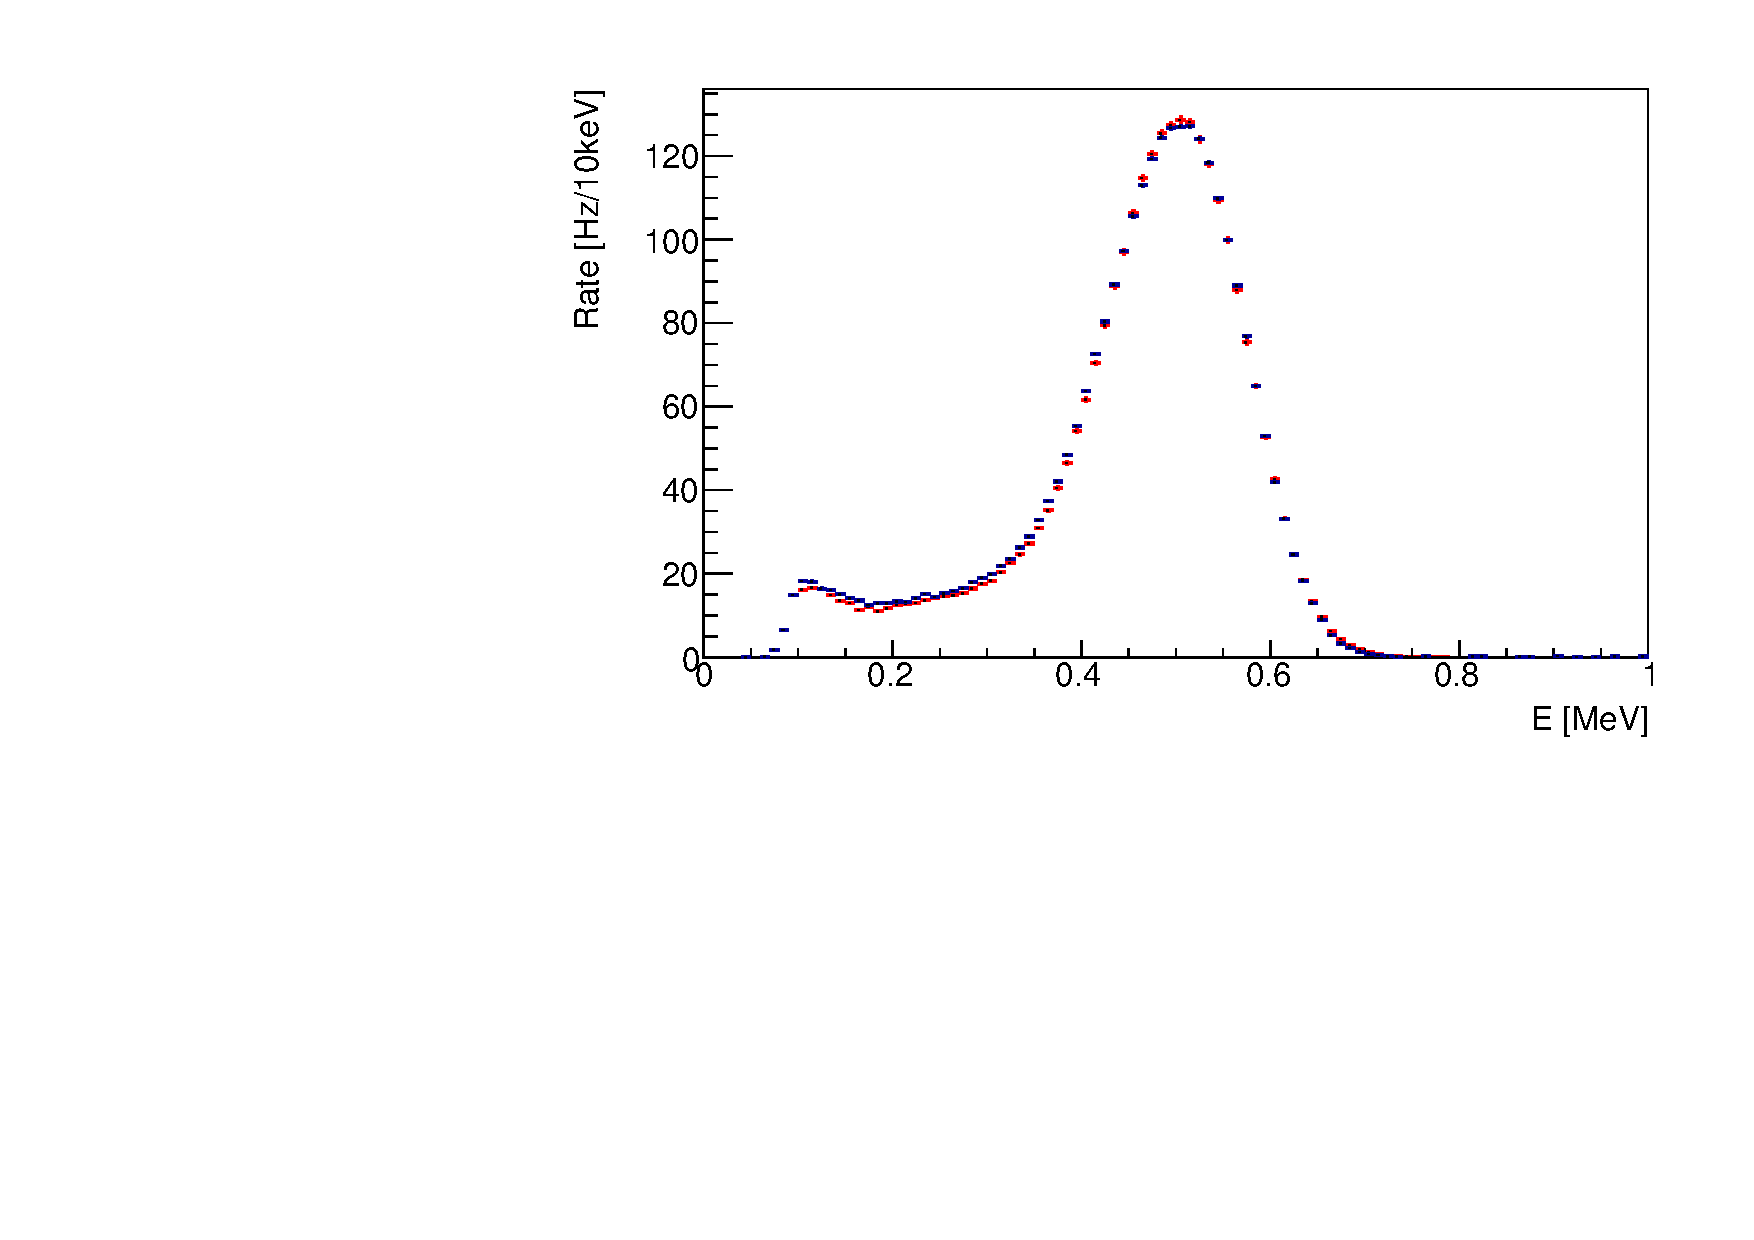
\includegraphics[width=60mm]{Figures/hCs137v2.pdf}}\quad
\subfigure[Full detector MC-data for $^{22}$Na calibration.]{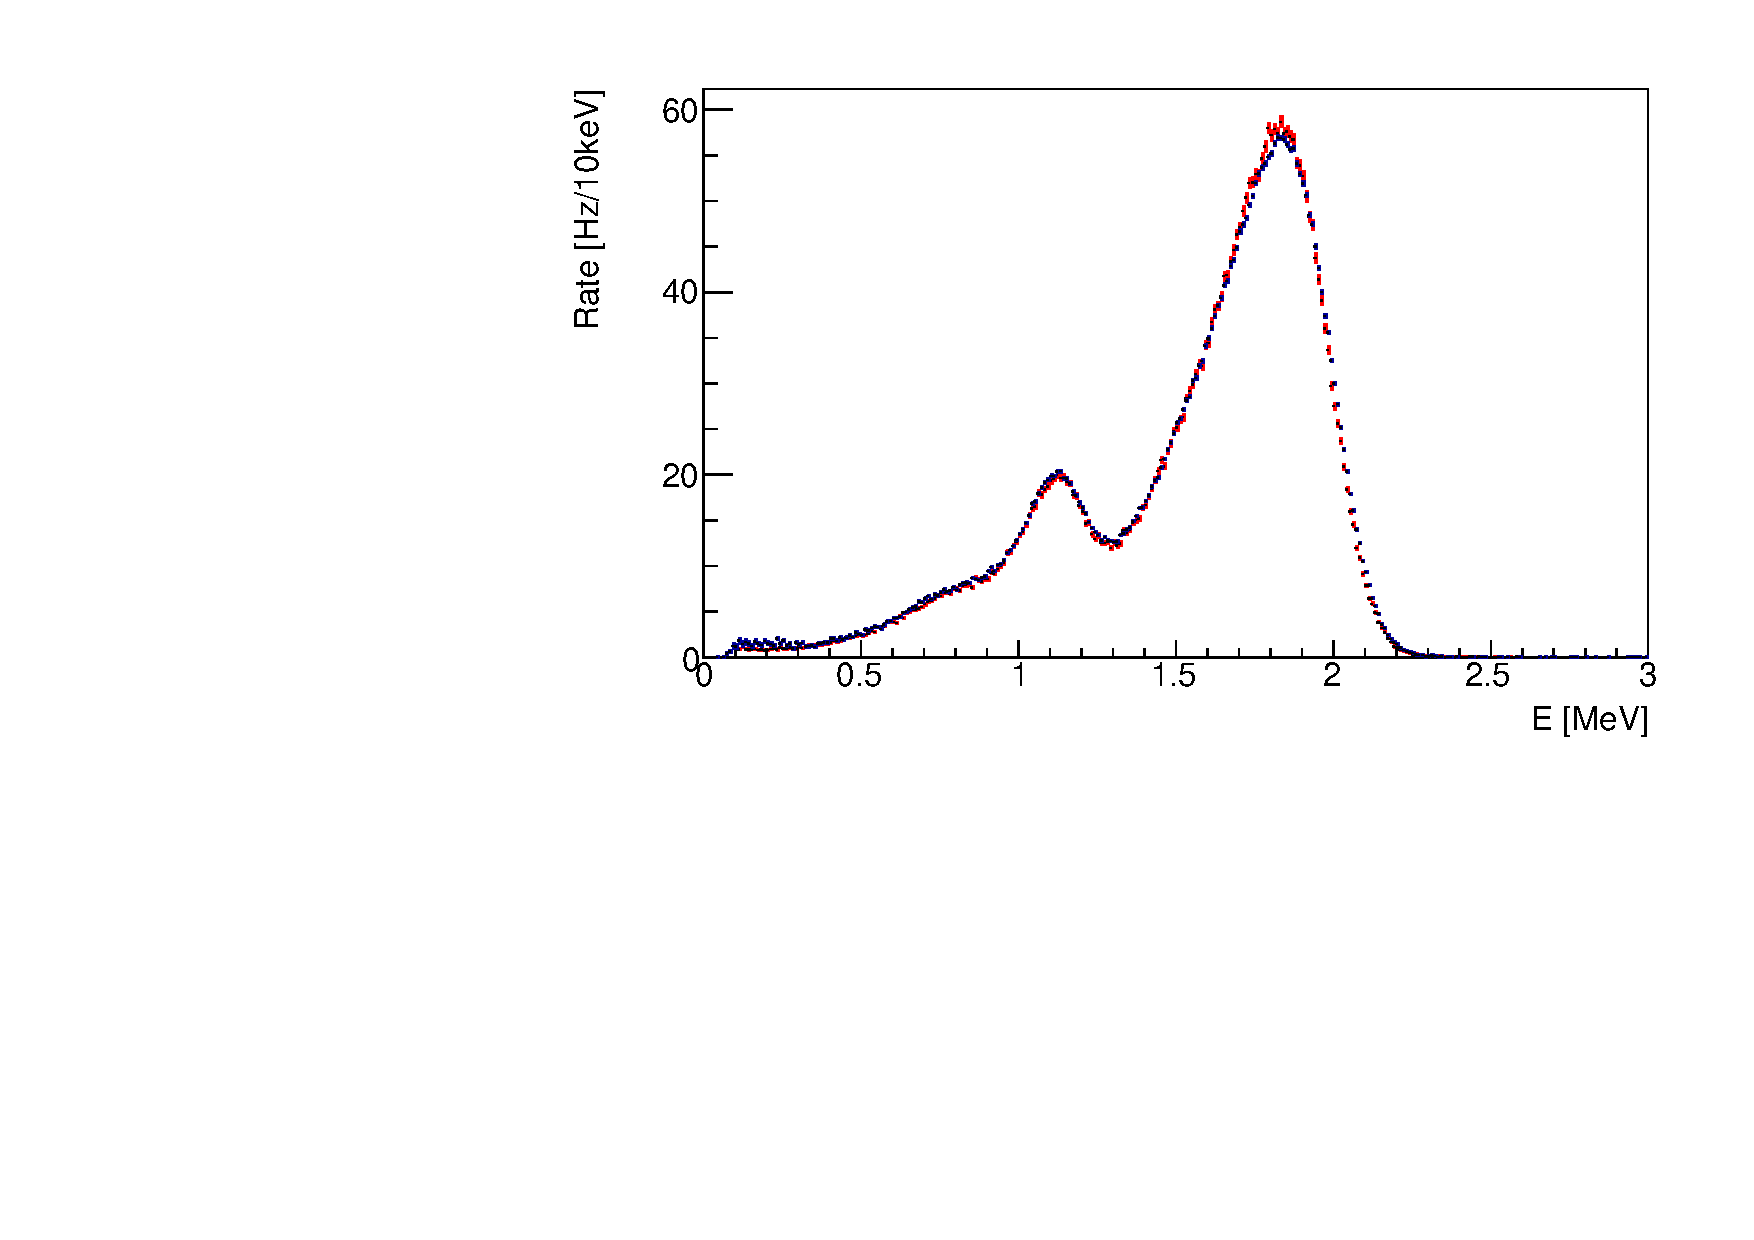
\includegraphics[width=60mm]{Figures/hNa22v2.pdf}} \\
\subfigure[Full detector MC-data for $^{60}$Co calibration.]{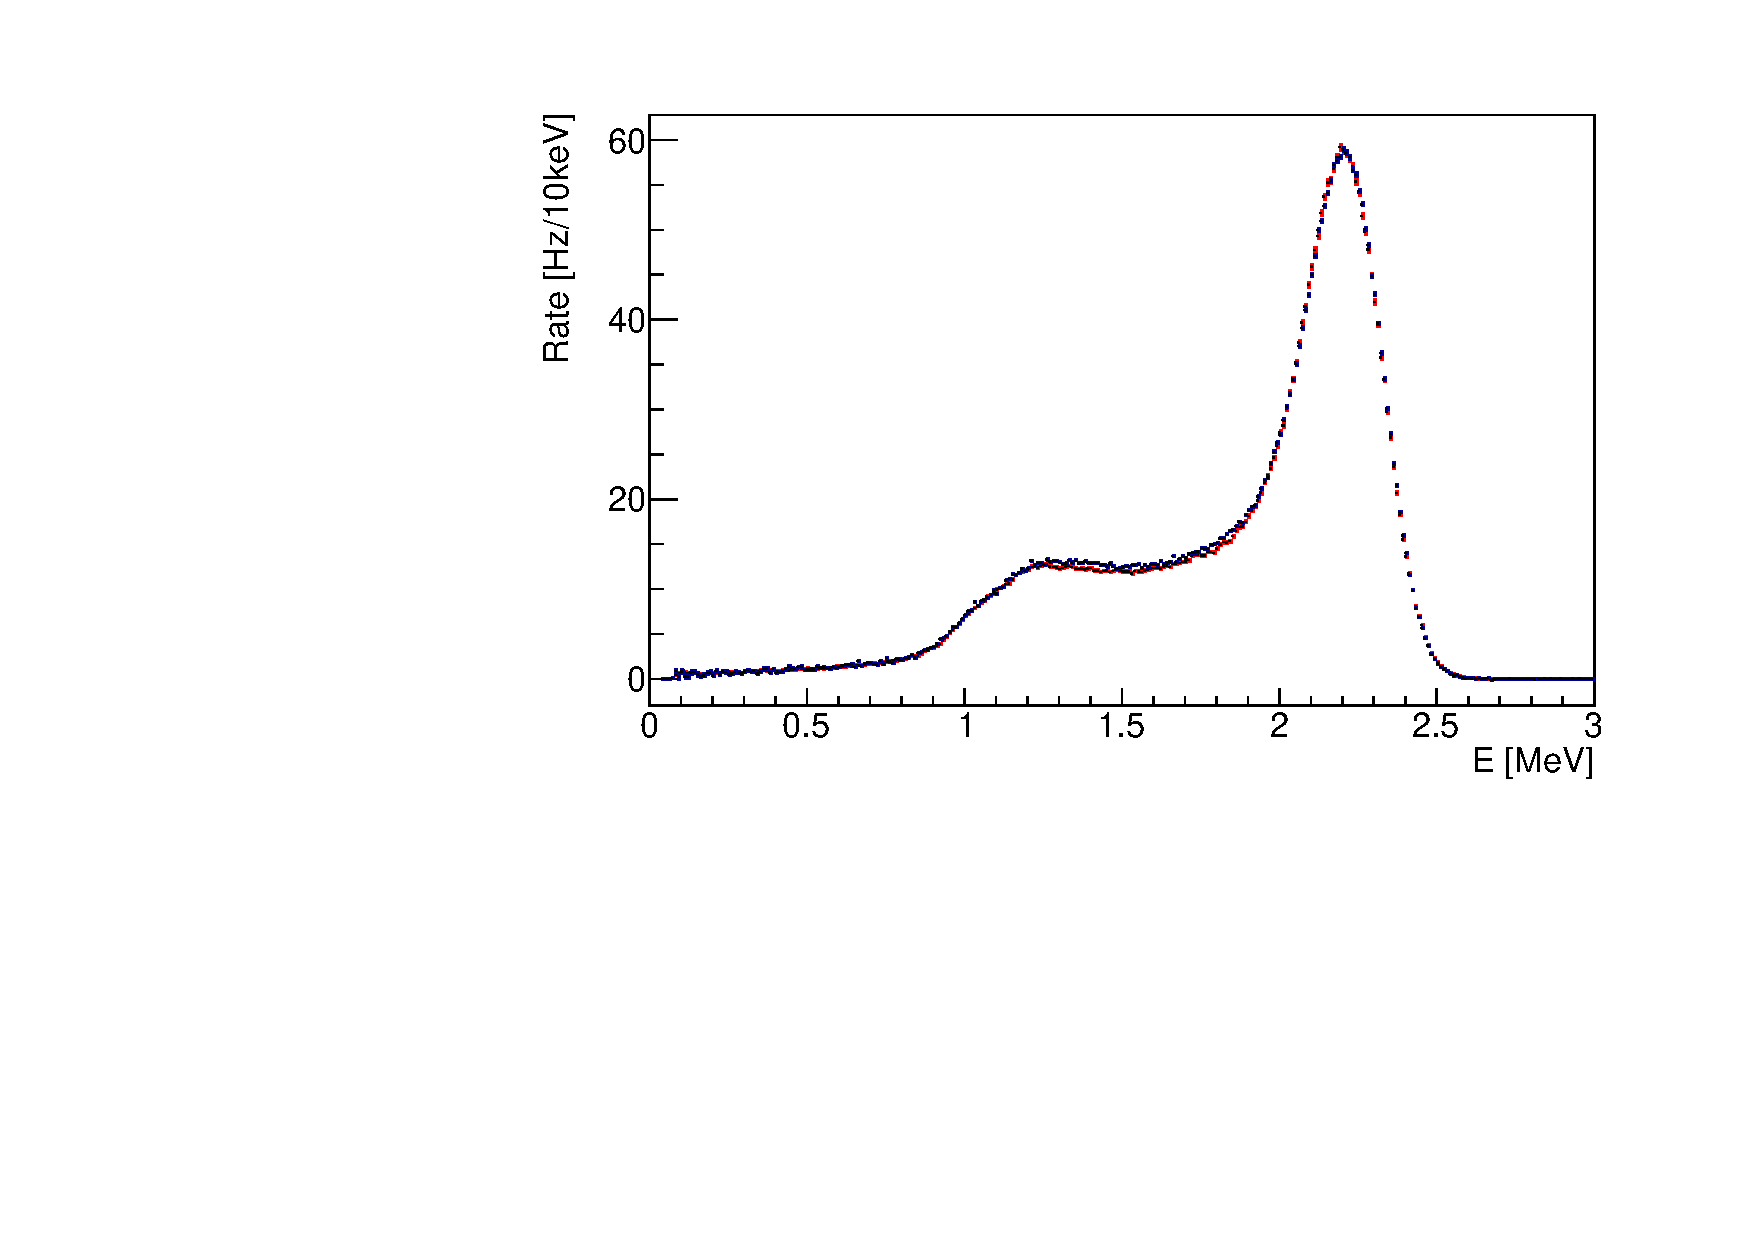
\includegraphics[width=60mm]{Figures/hCo60v2.pdf}} \quad
\subfigure[Full detector MC-data for n-H capture gamma.]{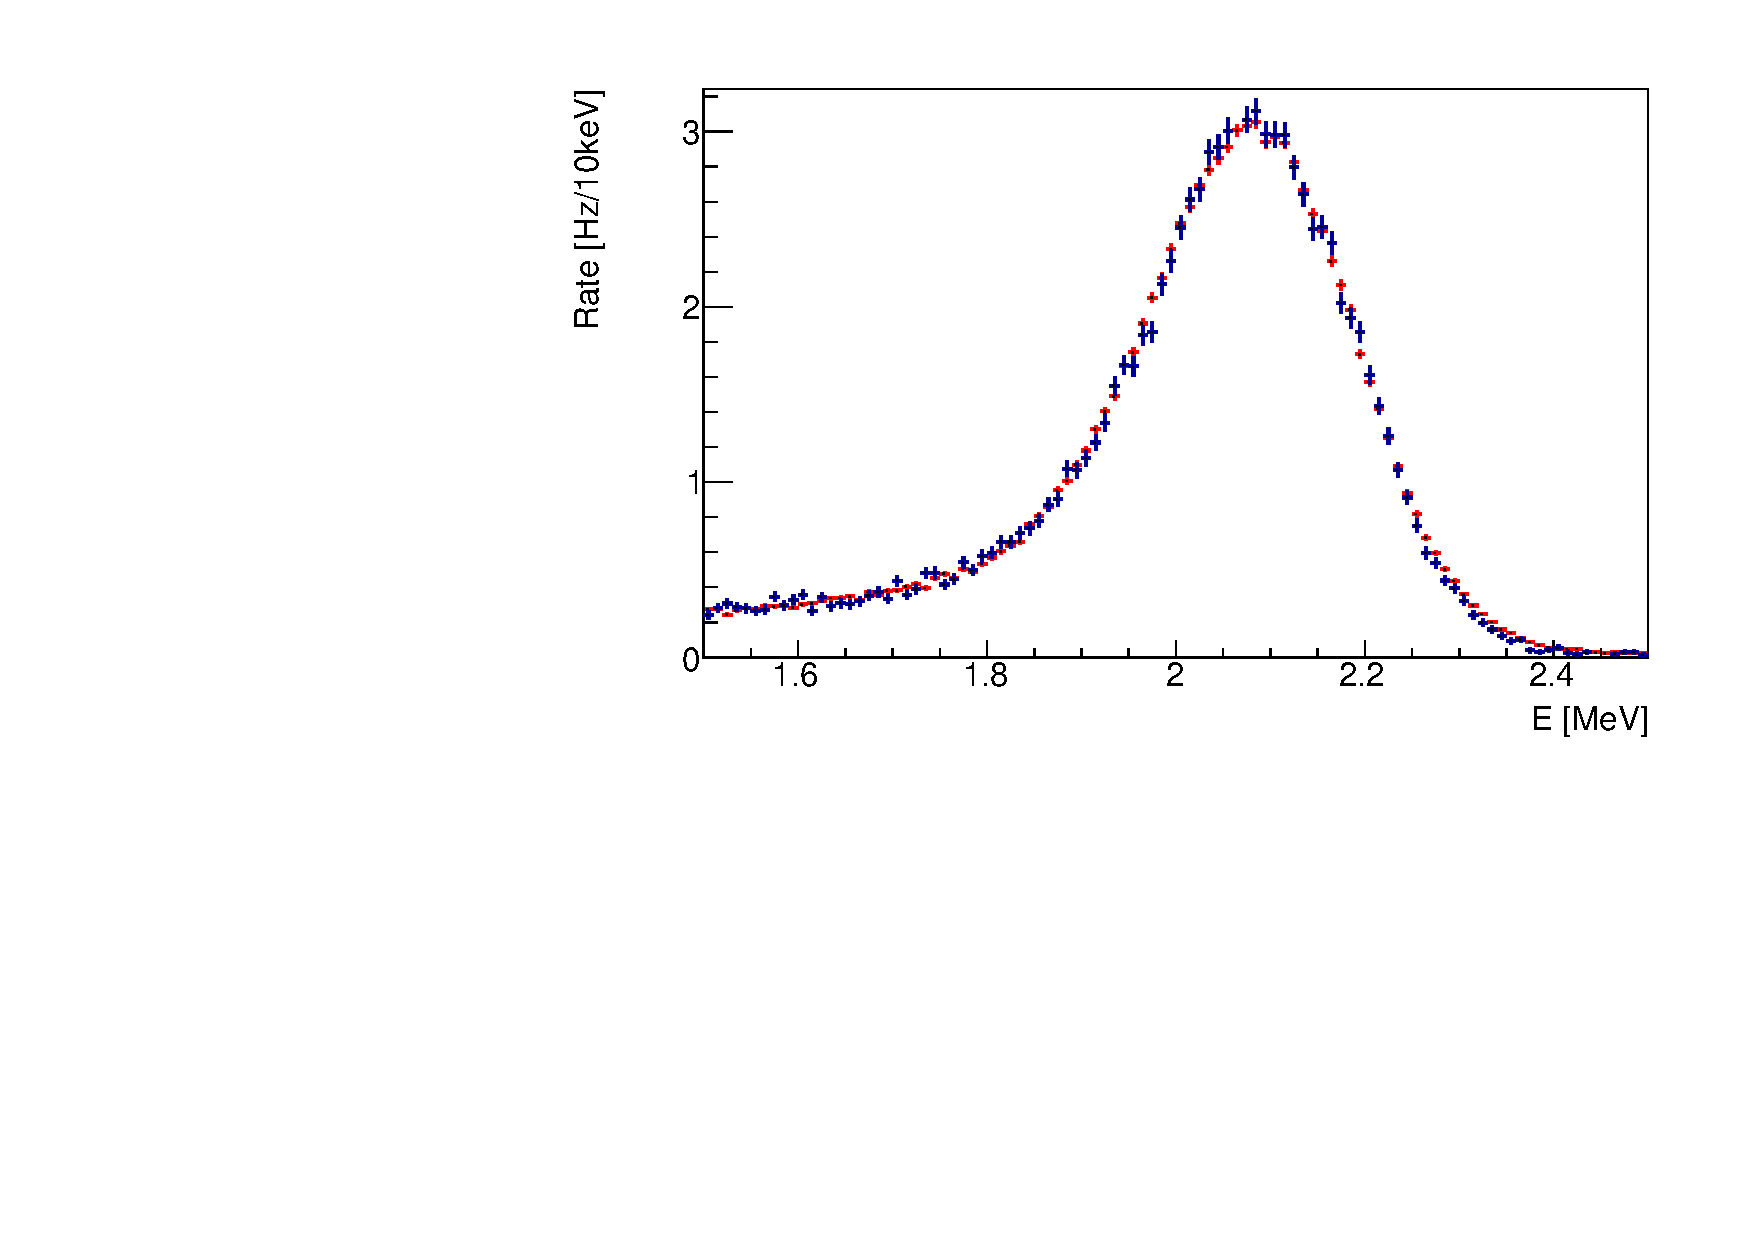
\includegraphics[width=60mm]{Figures/hCf252v2.pdf}} \\
\subfigure[Full detector MC-data for $^{12}$B spectrum.]{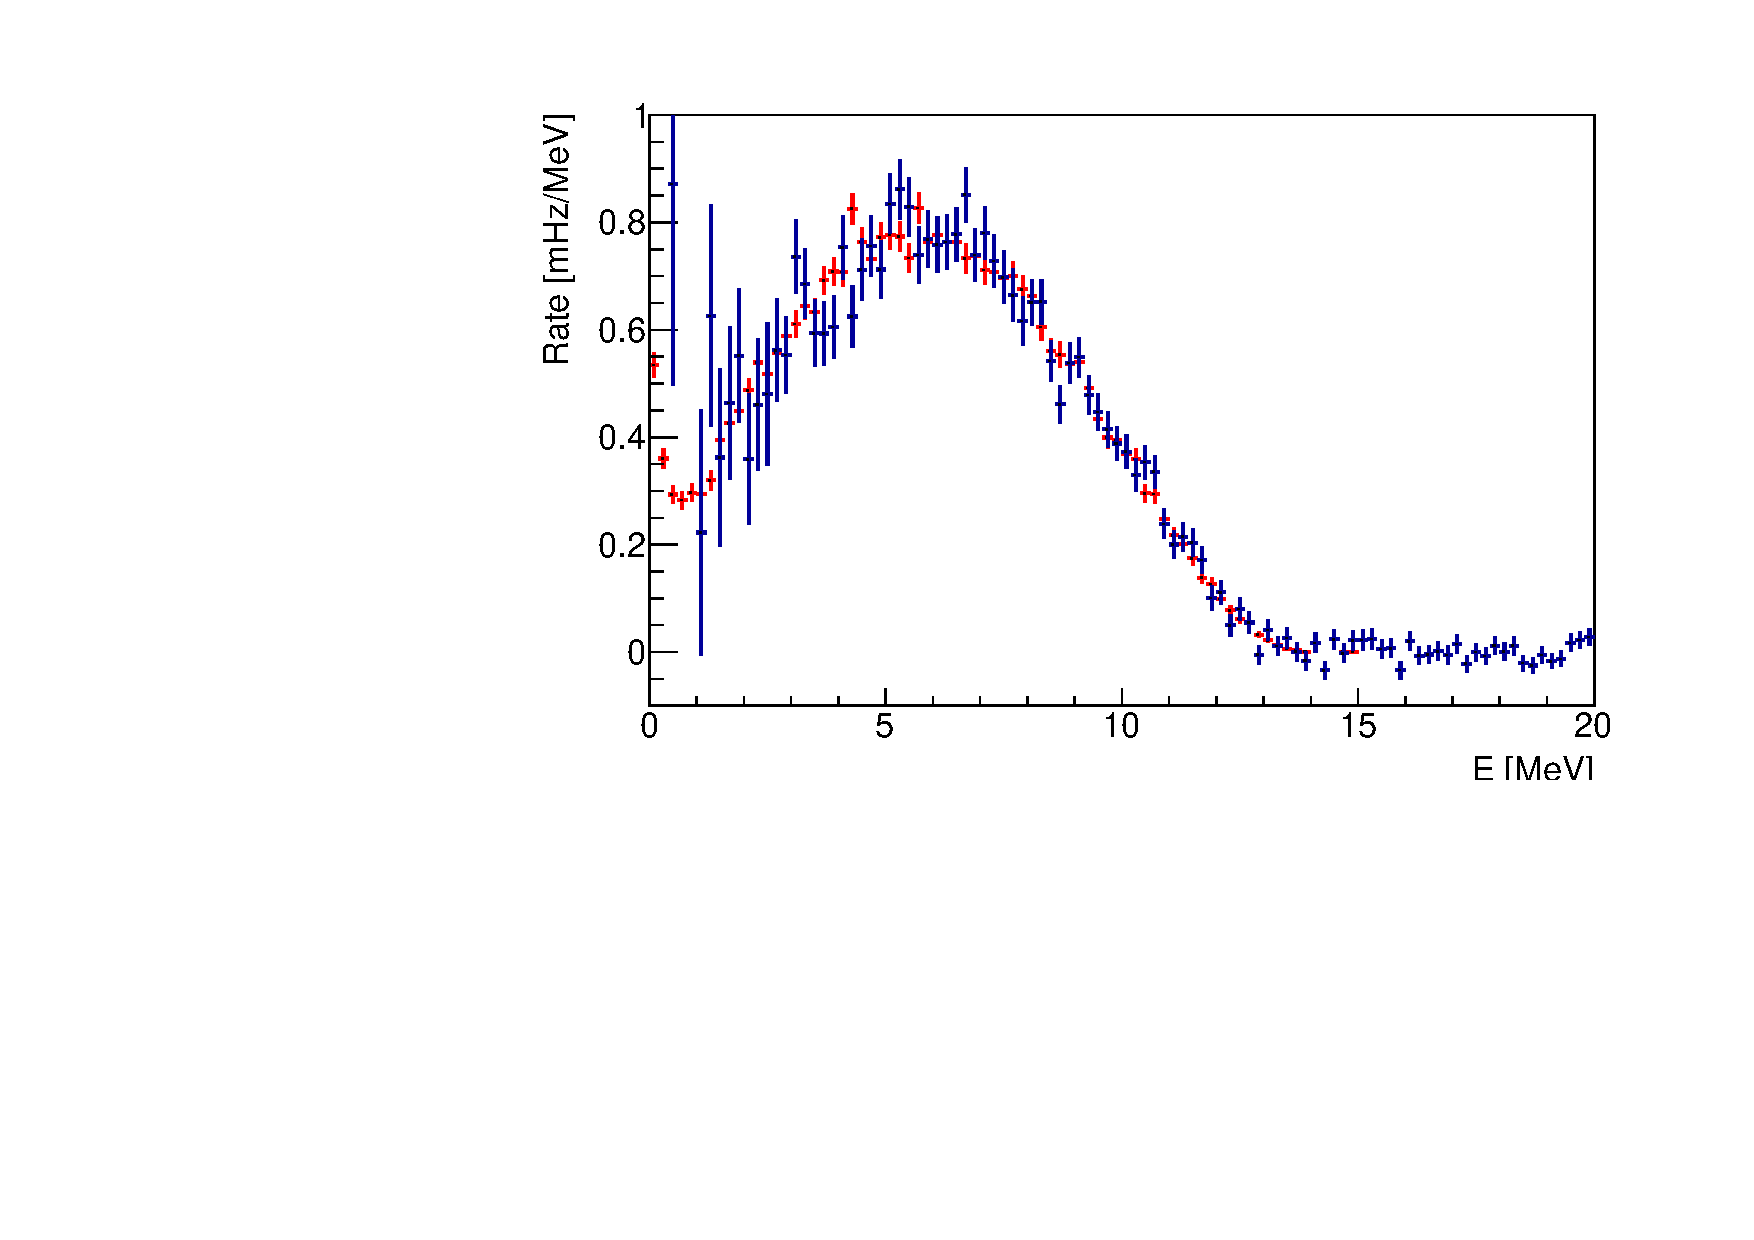
\includegraphics[width=60mm]{Figures/hB12v2.pdf}}

\caption{The full detector calibration energy spectra data vs MC. comparison, showing only statisitical error. (red: MC, blue: data)}
\label{fig:goodfit2}
\end{figure}

\begin{figure}[h!]
\centering
\subfigure[Full detector MC-data for $^{137}$Cs calibration.]{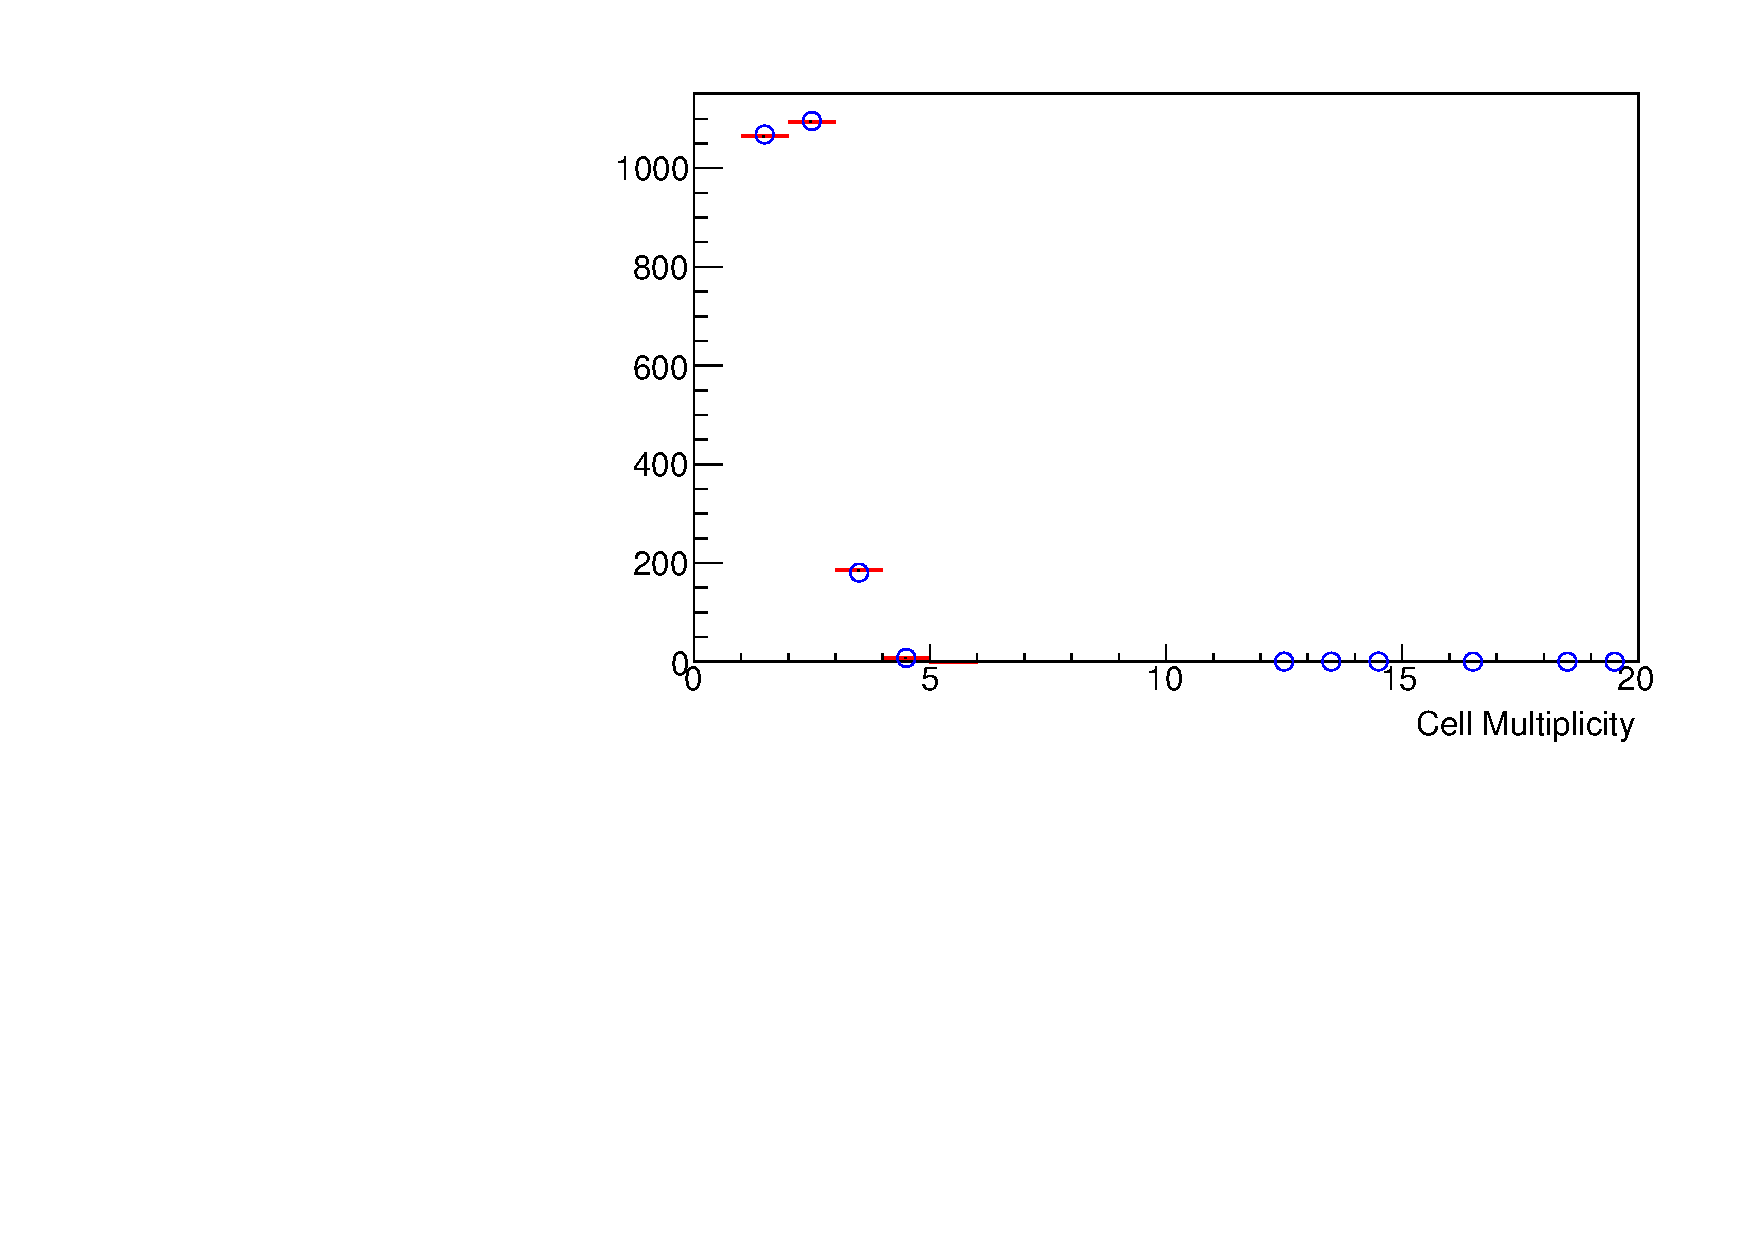
\includegraphics[width=60mm]{Figures/hCs137multi.pdf}}\quad
\subfigure[Full detector MC-data for $^{22}$Na calibration.]{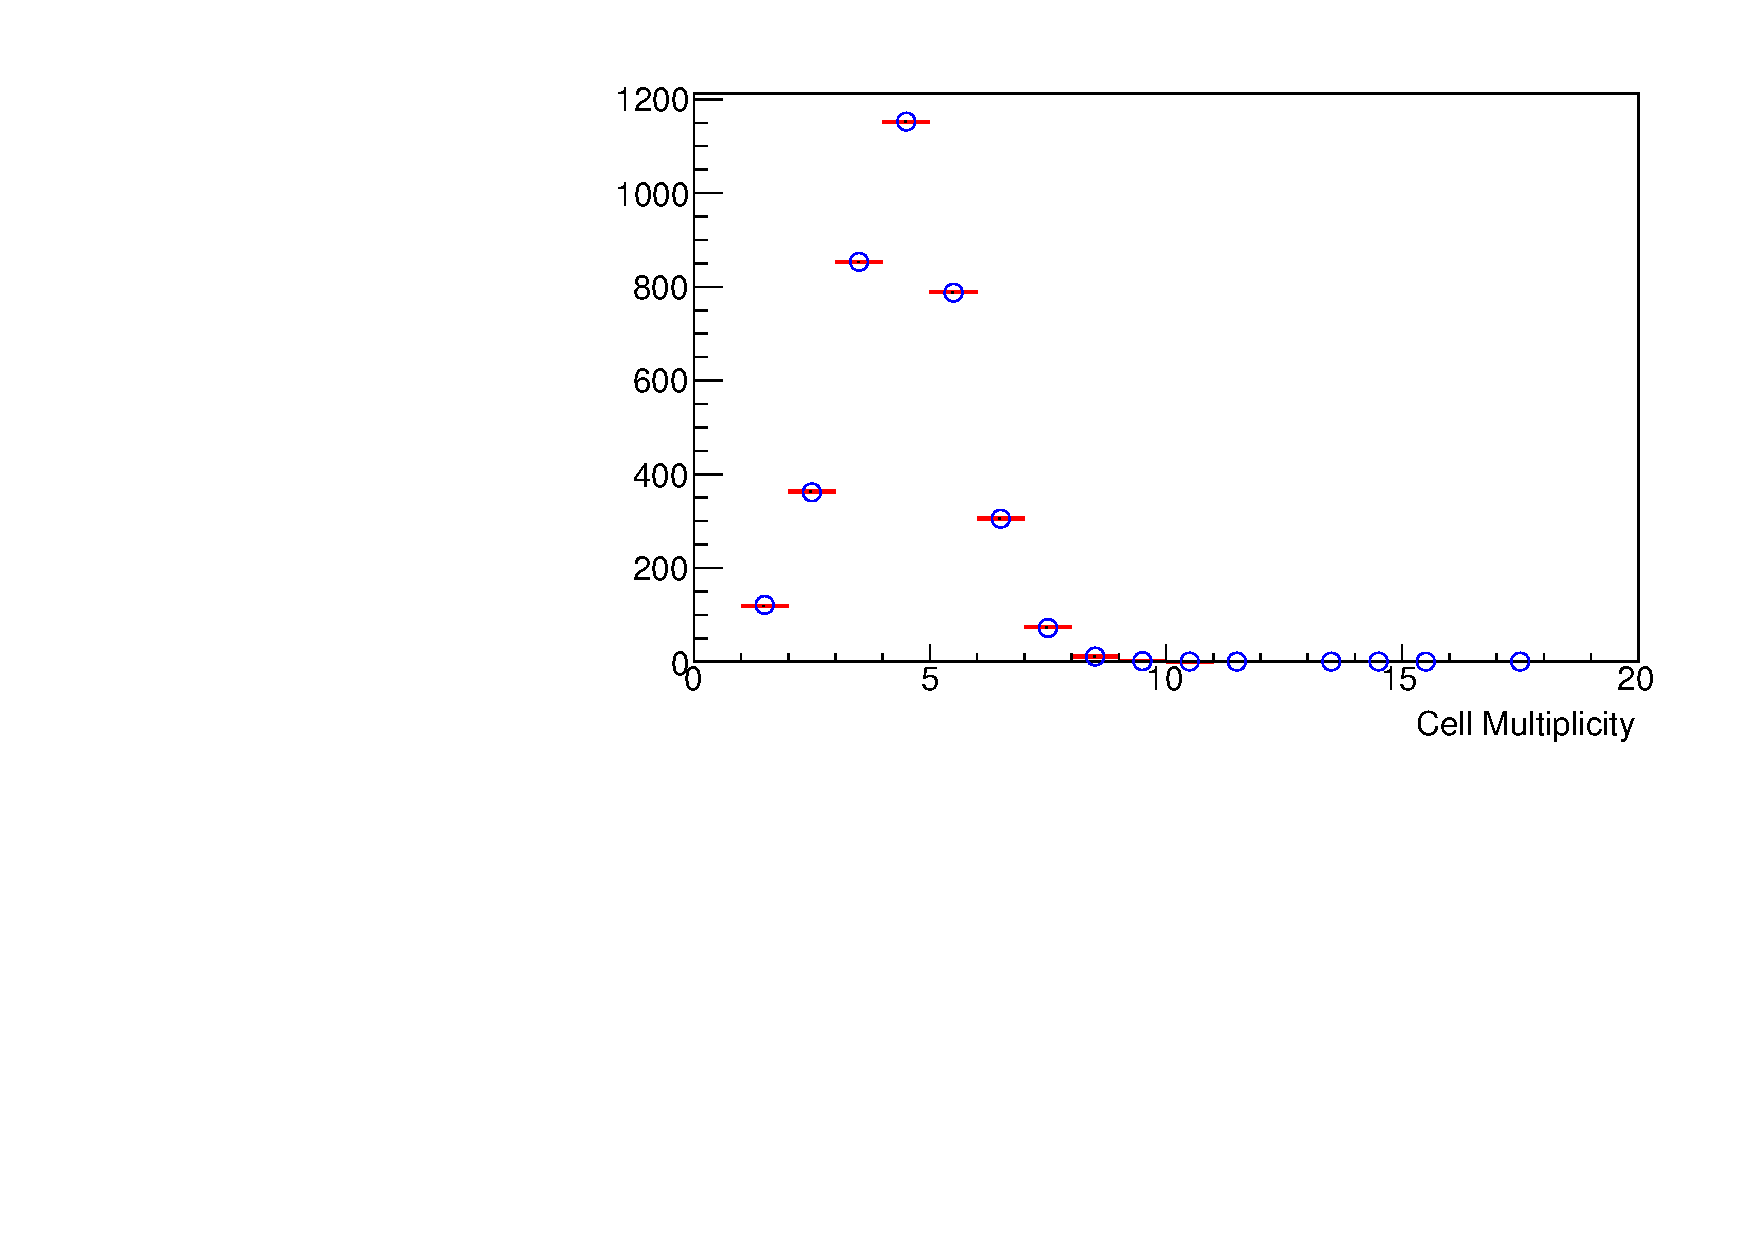
\includegraphics[width=60mm]{Figures/hNa22mulit.pdf}} \\
\subfigure[Full detector MC-data for $^{60}$Co calibration.]{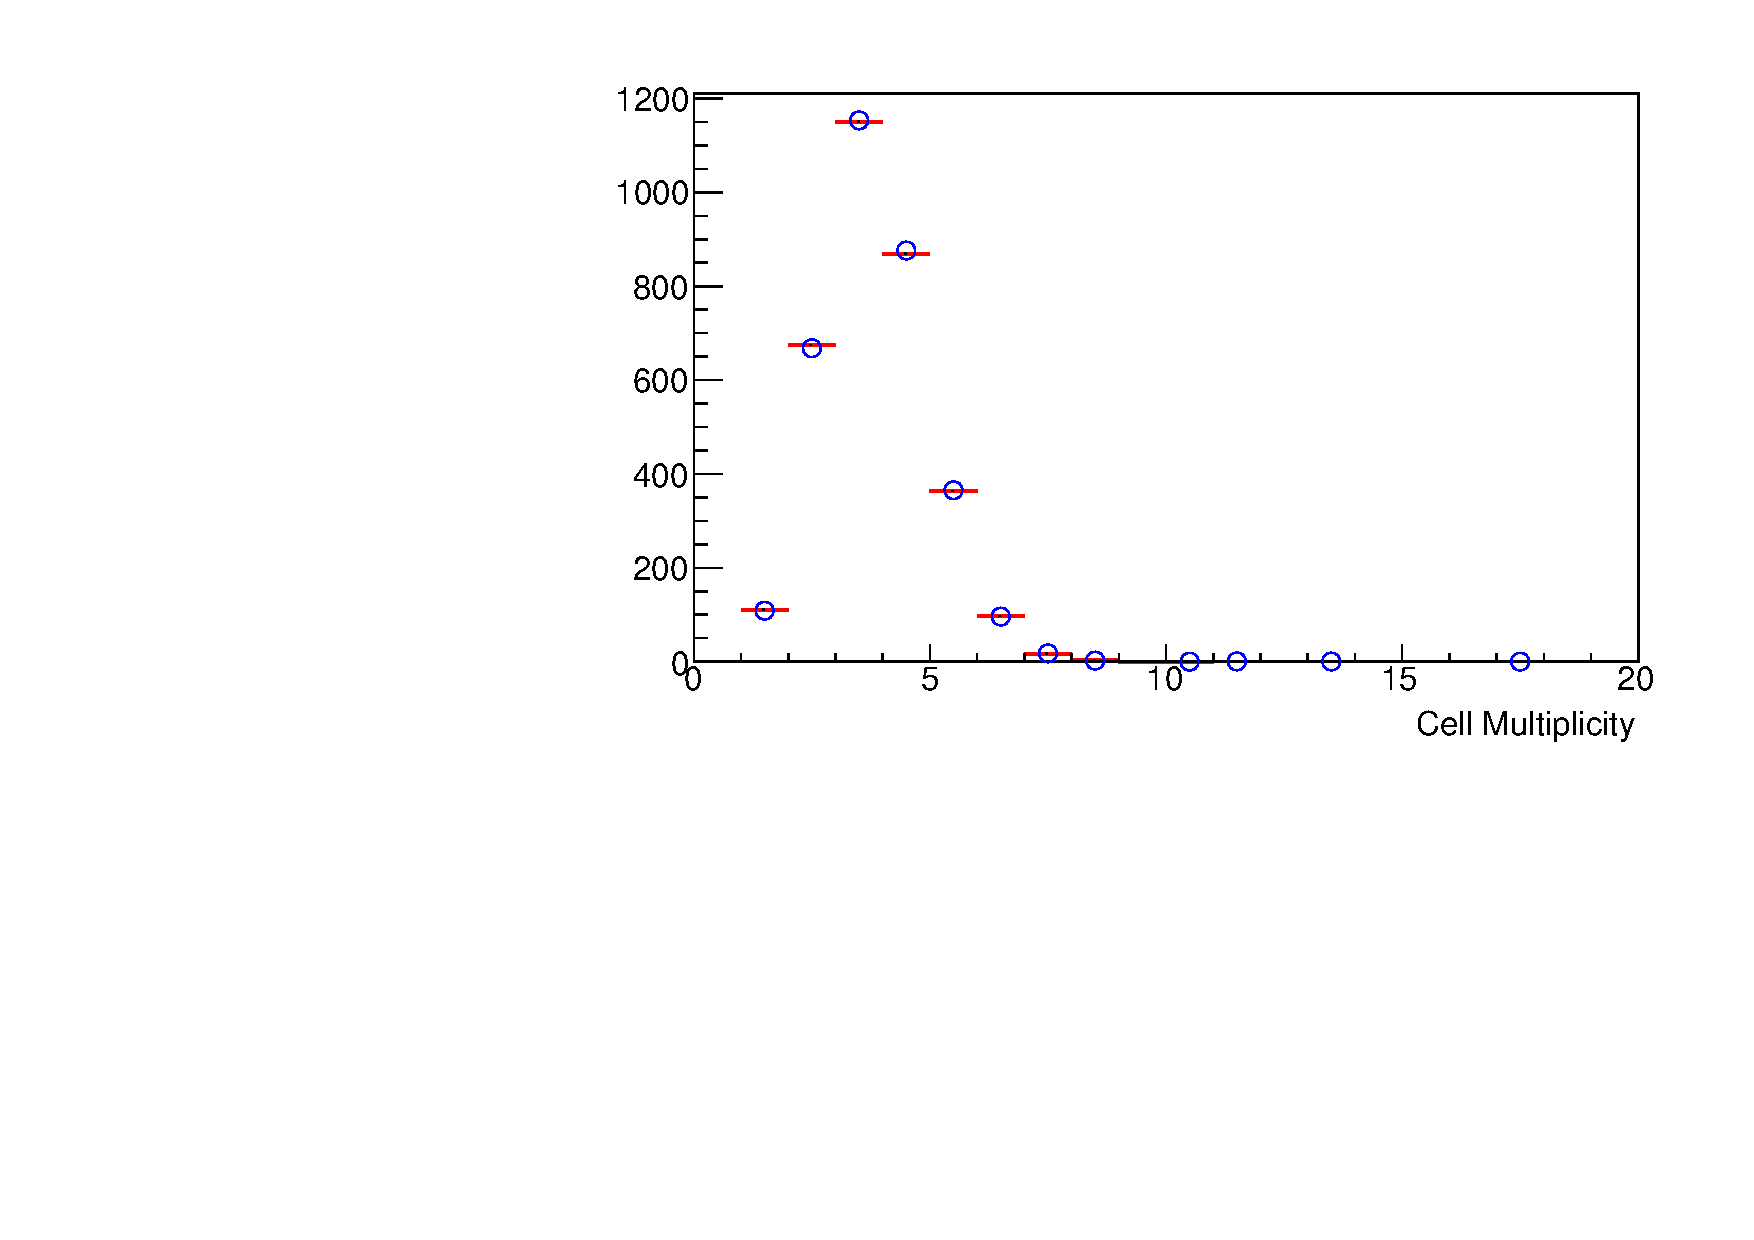
\includegraphics[width=60mm]{Figures/hCo60multi.pdf}} 
\caption{Multiplicity distribution of gamma calibrations. (red: MC, blue: Data)}
\label{fig:multi}
\end{figure}

\begin{figure}[h!]
\centering
\subfigure[$\chi^2$ distribution depedent on first order Birks constant and Cherenkov efficiency.]{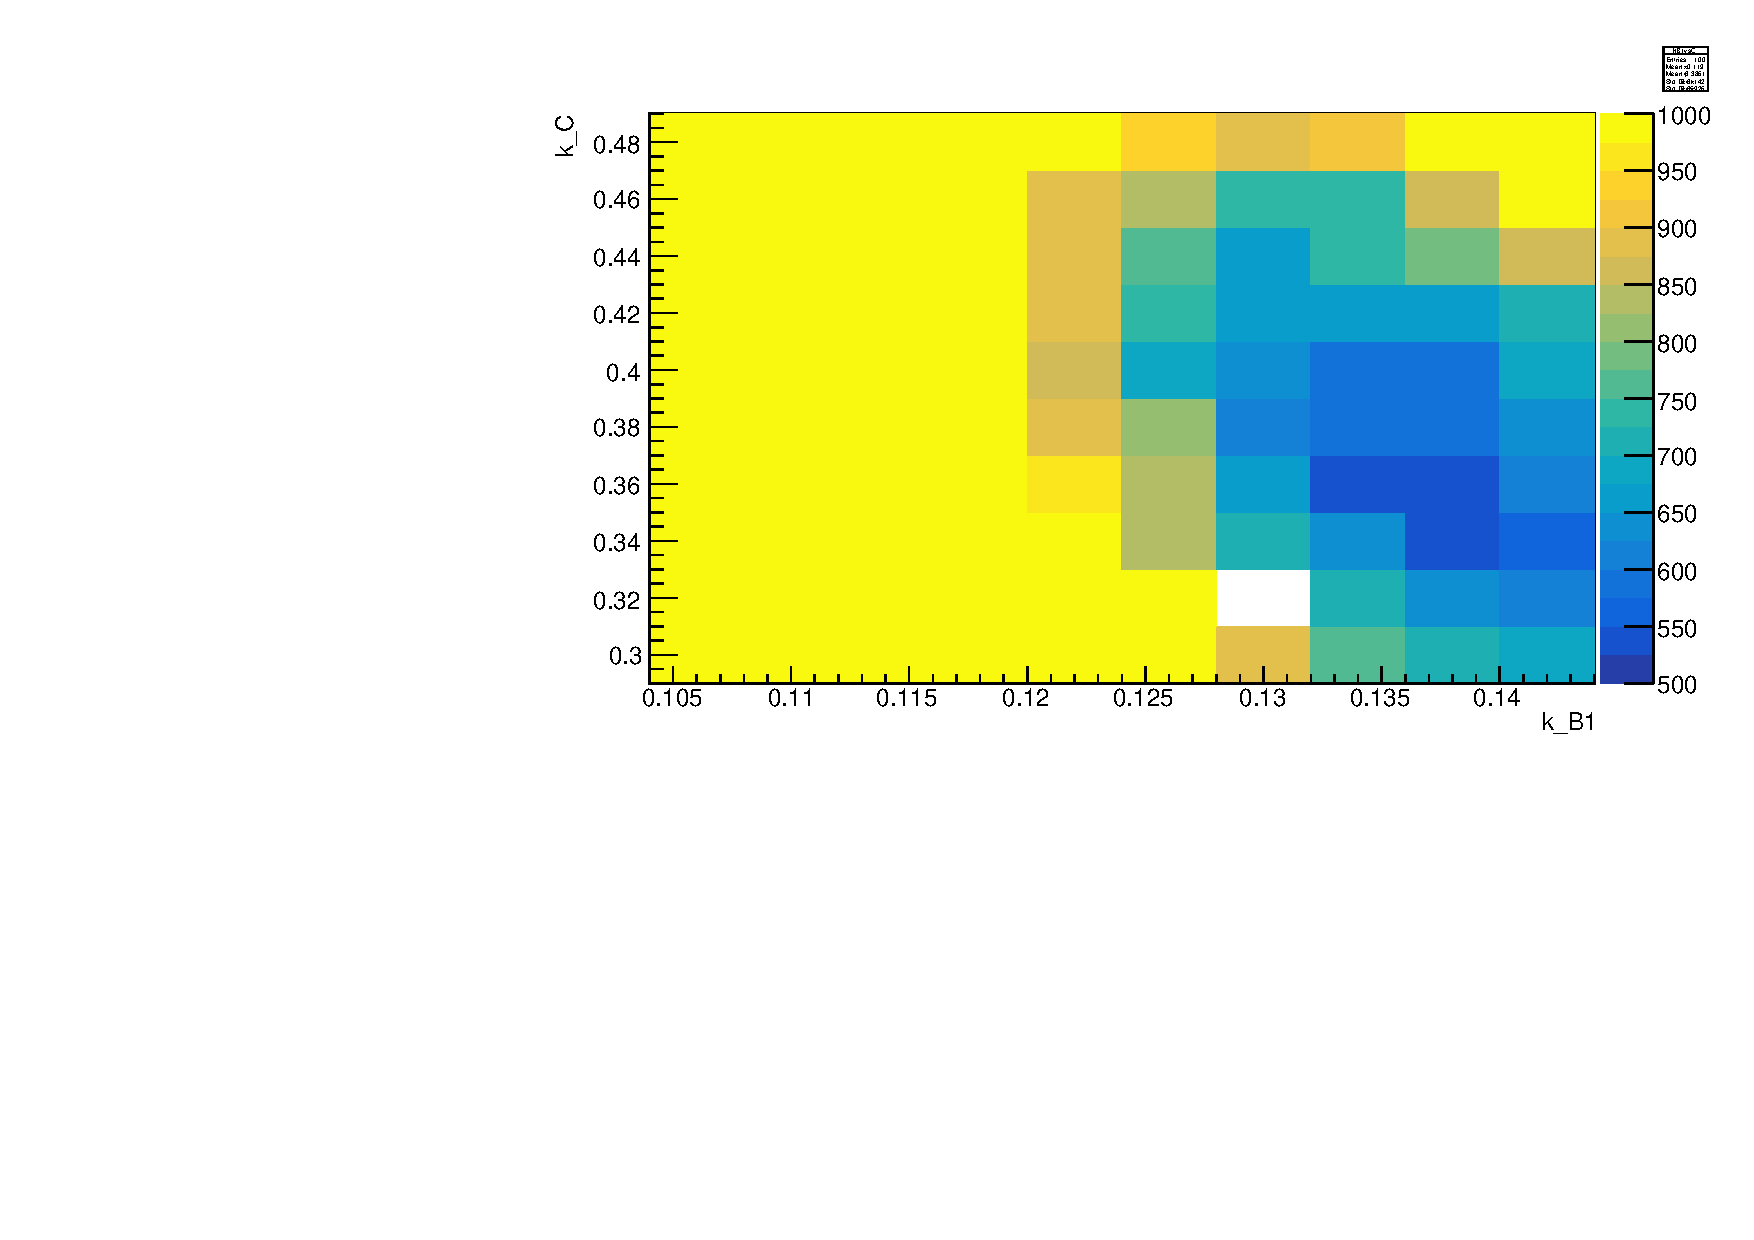
\includegraphics[width=70mm]{Figures/k1vkc.pdf}}\quad
\subfigure[$\chi^2$ distribution depedent on first order and second order Birks constant.]{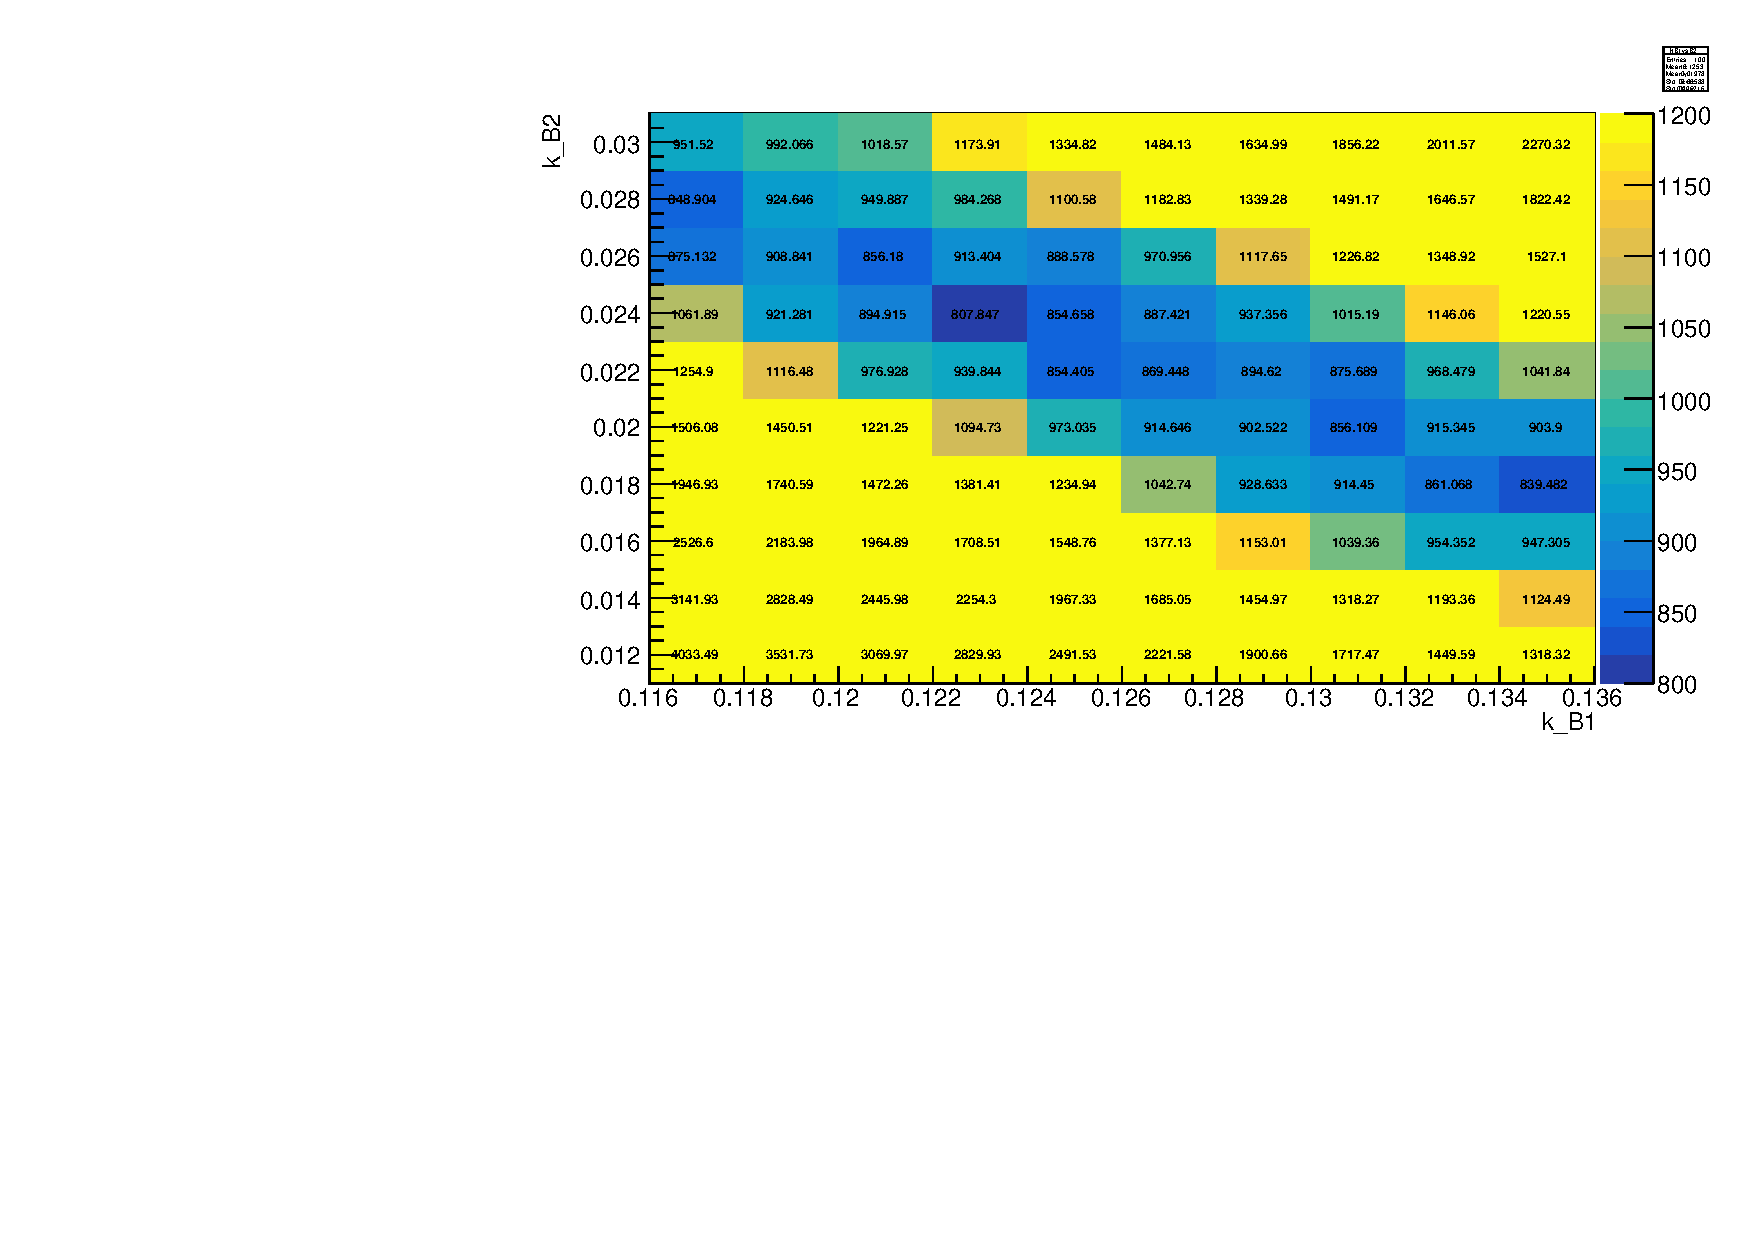
\includegraphics[width=70mm]{Figures/k1vk2.pdf}} \\
\subfigure[$\chi^2$ distribution depedent on second order and Birks constant and Cherenkov efficiency.]{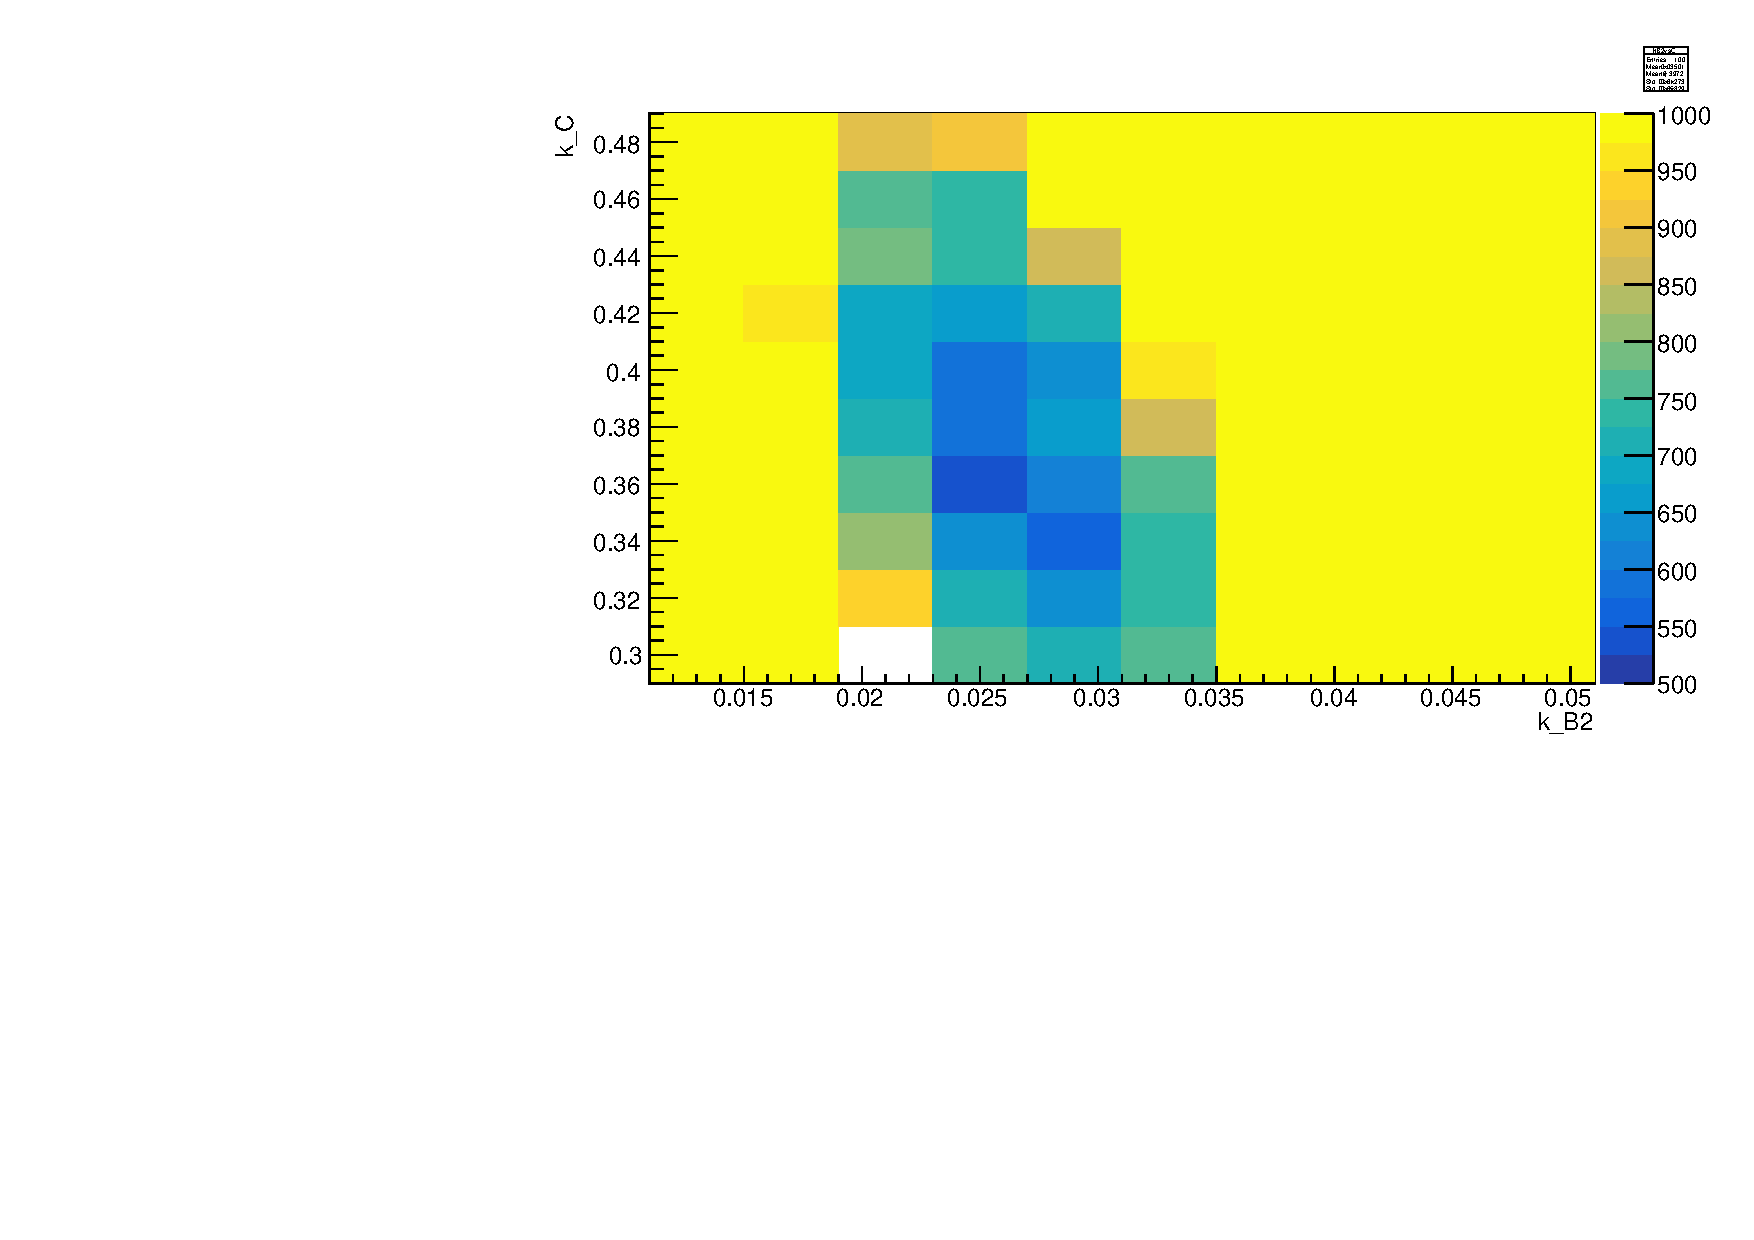
\includegraphics[width=70mm]{Figures/k2vkc.pdf}} 
\caption{$\chi^2$ distribution with respect to the values of nonlinearity parameters.}
\label{fig:chi2}
\end{figure}
\newpage
\clearpage

\Subsection{Single Cell Spectrum Comparison}
\label{sec:single}
The comparing the calibration spectra measured by only the single detector cells that are mostly adjacent to the calibration source can minimize the detector geometry correlated and the 85 keV thresholding effect for us to study LS nonlinearity.
The data and MC agreemnt in single-cell reconstructed energy is a good cross check of the full-detector best fit model.

Hence, we collected the single compton scattering gamma energy measured by only the single cells adjacent to the calibration sources respectively, four cells per source.
To reduce the systematic difference of energy scale between cells, the single hit gamma spectra from four cells were represented by the average spectrum of them. 
In gamma radioactive calibrations, the range of interest were from 0.2 MeV to the ends of spectra.
The range of fitting for gamma spectrum from n-H capture was 1.5 MeV to 2.3 MeV.
In single cell comparison, we compare only the single hit $^{12}$B electron energy spectrum.
The range of fitting for $^{12}$B spectrum is 3 to 13.5 MeV. 
To simplify the fitting, the MC spectra were normalized to data based on the spectral integral in the range of interest.
We performed the $\chi^2$ comparison to each of the calibraion spectra, and treat the sum of the $\chi^2$ values as combined $\chi^2$. 

The data vs. MC comparisons with full detector best fit are shown in Figure \ref{fig:goodfit}. 
The $\chi^2/NDF = 1425.4/420$ with the parameters nonlinearity model obtained in the full-detector fitting in Section \ref{sec:fulldet}, the overall energy shift is $\beta_{rec} = 0.40\%$.

\begin{figure}[h!]
\centering
\subfigure[Best-fit MC-data for $^{137}$Cs calibration.]{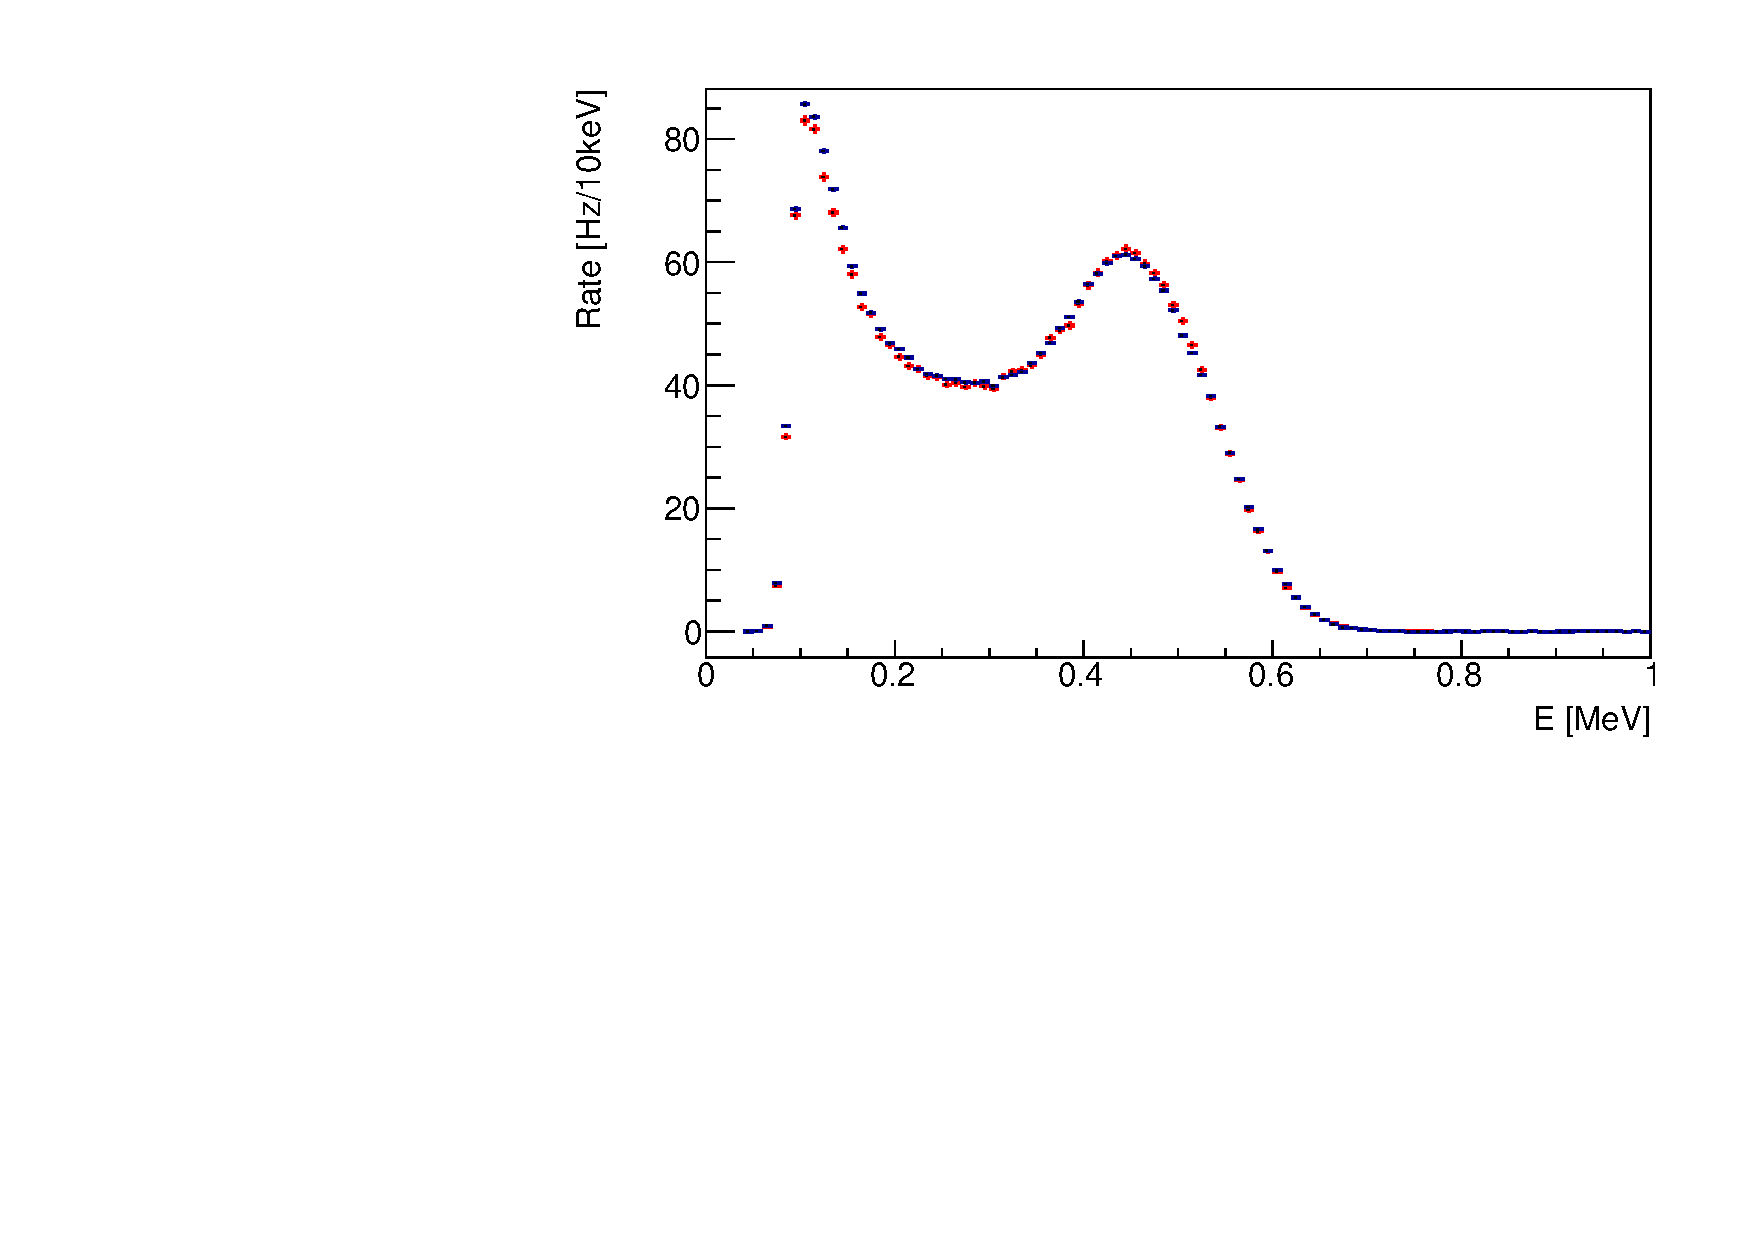
\includegraphics[width=60mm]{Figures/hCs137v2single.pdf}}\quad
\subfigure[Best-fit MC-data for $^{22}$Na calibration.]{\includegraphics[width=60mm]{Figures/hNa22v2single.pdf}} \\
\subfigure[Best-fit MC-data for $^{60}$Co calibration.]{\includegraphics[width=60mm]{Figures/hCo60v2single.pdf}} \quad
\subfigure[Best-fit MC-data for n-H gamma.]{\includegraphics[width=60mm]{Figures/hCf252v2single.pdf}} \\
\subfigure[Best-fit MC-data for $^{12}$B]{\includegraphics[width=60mm]{Figures/hB12v2single.pdf}} 
\caption{The best fit results from single-cell data vs. MC comparison.}
\label{fig:goodfit}
\end{figure}
\newpage
\clearpage

\Subsection{Agreement Among Different Calibration Campaigns}
The energy scale model discussed in previous sections were found with combined fitting of gamma calibrations taken in April 2018, neutron calibration performed in May 2018 and ambient data. 
Idealy, this model ought to be compatible with other calibration campaigns with same configuration. 
Thus we applied the model to the August 2018 calibration, which includes both gamma and neutron calibrations, as a further cross check on the best fit model.
An issue with the August 2018 calibration is that one source was possibly partially left between the detector and shielding volume, shown in Figure \ref{fig:left}.

\begin{figure}[h!]
\centering
\includegraphics[width=80mm]{Figures/secondhotspot.png}
\caption{The event distribution of gamma event cluster, there is a secondary hot spot indicating another source trapped in the volume between detector volume and shielding.}
\label{fig:left}
\end{figure}

To avoid the contamination from the source, instead of measure the full-detector reconstructed energy, the event selection constrained every hits of a cluster being within 3 layers of LS cell from the center, showed in Figure \ref{fig:ring}.
To maintain uniformity in energy spectrum comparison, we applied the 3-layer energy reconstruction on both the April gamma calibration and August gamma calibration, while made neutron calibration and ambient calibration remain-full detector reconstruction because they were not affected by the trapped source.

\begin{figure}[h!]
\centering
\includegraphics[width=80mm]{Figures/Ring.png}
\caption{An example of how 3 layers of LS was defined.}
\label{fig:ring}
\end{figure}

When we reapplied the best-fit nonlinearity model to the April data-MC comparison with 3-layer reconstruction, the total $\chi^2$ value increased from 807.847 to 1082.1, and absolute energy scale shifted from 0.36\% to 0.42\%, indicating unresolved multiplicity disagreement between MC and data.
The $\chi^2/NDF = 2750.78$ when the same model was deployed in August calibration data-MC comparison, with absolute energy scale shift = 0.32
However, as shown in Figure \ref{fig:compare}, the energy scale at discrepancy is within 0.8\% uncertainty.

\begin{figure}[h!]
\centering
\includegraphics[width=80mm]{Figures/EScaleCompare.pdf}
\caption{The discrepancy between April and August calibration energy scale is within $\sim0.8\%$ uncertainty.}
\label{fig:compare}
\end{figure}

\newpage

\Section{Final Model and Uncertainties for the Spectrum Analysis}
According to Section \ref{sec:dataMC}, we finalized the energy nonlinearity model based on the single-cell data vs. MC comparison.
The energy scale of PROSPECT AD can be expressed as the ratio of true energy to reconstructed energy of average particle from different calibrations $E_{rec}/E_{true}$ as shown in Figure \ref{fig:escale}, which indicates at lower energy, the scale is able to vary $\sim0.8\%$ from 100\%, where 0.2\% came from energy scale fluctuation caused by nonlinearity model uncertainty, the 0.6\% will be discussed in the next paragraph.

\begin{figure}[h!]
\centering
\includegraphics[width=80mm]{Figures/EScale.pdf}
\caption{The reconstructed energy to true energy ratio.}
\label{fig:escale}
\end{figure}

The $^{12}$B energy spectrum data vs MC comparison was used to demonstrate the energy scale at higher energy, shown in Figure \ref{fig:B12final}. 

\begin{figure}[h!]
\centering
\subfigure[Full detector MC-data comparison for $^{12}$B spectrum.]{\includegraphics[width=60mm]{Figures/hB12v2.pdf}} \quad
\subfigure[The residual of this comparison.]{\includegraphics[width=60mm]{Figures/hB12residualv2.pdf}} \quad
\caption{The average residual of this comparison found the to be $0.49 \pm 0.60\%$}
\label{fig:B12final}
\end{figure}

The energy resolution in Figure \ref{fig:resolution} shows the resolution of each energy distributions of calibrations, fitted with Function \ref{eql:resolution}.

\begin{figure}[h!]
\centering
\includegraphics[width=80mm]{Figures/Resolution.pdf}
\caption{The energy resolution of mean energies of each calibration fitted with resolution function. (errors are currently statisical only)}
\label{fig:resolution}
\end{figure}

The data vs. MC comparison of $^{22}$Na gamma spectrum is a good way to indicate the multi-particle event reconstructino of PROSPECT AD, see Figure \ref{fig:Na22final}.

\begin{figure}[h!]
\centering
\subfigure[Full detector data-MC comparison for $^{22}$Na calibration.]{\includegraphics[width=60mm]{Figures/hNa22v2.pdf}} \quad
\subfigure[The residual of this comparison.]{\includegraphics[width=60mm]{Figures/hNa22residual.pdf}} \quad
\caption{The data-MC comparison of $^{22}$Na spectrum and residual of comparison.}
\label{fig:Na22final}
\end{figure}

\newpage
The gamma calibration sources supplied sufficient amount of statistics. 
The $0.60\%$ energy scale uncertainty and statistical uncertainty of $^{12}$B spectrum smeared the $\chi^2$ distribution during the quenching model search, thus enlarged uncertainty of nonlinearity model. 
We chose to be conservative and treat the 0.6\% energy scale uncertainty in $^{12}$B as an systematic energy scale uncertainty.
The energy resolution in spectrum analysis are forced to be smeared with respect to the poorest resolution measured in detector during data taking.

In conclusion, the uncertainty of energy response is dominated by the systematic uncertainties:

\begin{itemize}
    \item The $1-\sigma$ uncertainty of Birks$^\prime$ constants and Cherenkov efficiency.
    \item The 0.6\% uncertainty of absolute energy scale.
    \item The thresholding uncertainty of $85\pm5$ keV.
    \item The uncertainty of the artificial smearing $400\pm8$ PE/MeV.
    \item The uncertainty of thickness of separator of $1.18\pm0.05$ mm.
\end{itemize}
Each of the uncertainties above are turned into covariance matrix individually. 
As a result, the covariance matrices of energy scale uncertainty and thickness of separator are shonwn in Figure \ref{fig:cov}.

\begin{figure}[h!]
\centering
\subfigure[Covariance matrix for the uncertainty in nonlinearity and energy scale model.]{\includegraphics[width=60mm]{Figures/nonlinearcov.pdf}} \quad
\subfigure[Covariance matrix for the uncertainty of panel thickness.]{\includegraphics[width=60mm]{Figures/thickcov.pdf}} \quad
\caption{Current reduced covariance matrices.}
\label{fig:cov}
\end{figure}

\Section{Conclusion}

We are able to finalize the dominant parameters in energy scale study, which are $k_{B1} = 0.122 \pm 0.002$ mm/MeV, $k_{B2} = 0.032 \pm 0.002$ mm/MeV, $k_C = 41 \pm 1\%$, $\beta_{rec} = 100.36\pm0.6\%$.
The uncertainties in energy scale is mainly the uncertainty of parameters and separator thickness.
There are unresolved disagreement between full-detector best fit and single-cell best fit as well as multiplicity discrepancy that hinted further adjustments on detector geometry or material property.


\Section{Radioactive Source Calibrations}

\Section{Cosmogenic Calibration}

\Section{Data-model Comparison}

\Section{Energy Resolution}

\Section{Energy Resolution Stability}

\Section{Reconstruction Energy Scale}

\Section{Energy Scale Stability}

\Section{Position Dependence of Energy Scale}

\Section{Gamma Energy Loss}

\Section{Detector Response Matrix}

\Section{Uncertainty Propagation and Covriance Matrices}

\Chapter{Absolute Energy Scale Calibration}
\label{Ch8}

The reactor neutrino spectrum measurement of PROSPECT relies on correct reconstruction of IBD prompt positron energy of IBD events. 
The absolute energy scale ought to be precisely calibrated for this physics goal.

The reconstructed energy with the PROSPECT AD is naturally different from the energy deposited by particles because of energy loss, light leakage, imperfection of detector components, and nonlinear effects.
Most of these effects are simulated with PG4.
It is vital to characterize the detector response with correctly simulated detector structure, nonlinearity of energy response and energy resolution to
\begin{itemize}
    \item Supply an accurate nonlinear detector response model to the MC.
    \item Quantify the systematic uncertainty in energy response. 
\end{itemize}

In the absolute energy scale calibration, gamma sources, neutron sources calibration and ambient data calibration were used to characterize the absolute detector response, including nonlinearity contributed by the Birks' law quenching and Cherenkov radiation of scintillator, and absolute energy scale adjustments necessitated by the low level calibration presumption of $n$-Li visible energy (described in Chapter~\ref{Ch7}). 
The corrected $n$-Li visible energy was re-calibrated based on the adjustment, while the stability of event reconstruction were also validated.

In addition, necessary detector geometry corrections were implemented, respect to physical measurements on detector material and dimensions to enhance data-MC agreement in gamma collection.
At last, the combined fit of all calibration data to PG4's MC simulation was made to constrain  the energy resolution and nonlinearity model.
This model, along with reactor neutrino production models, is used to produce a predicted IBD prompt energy spectrum from HFIR.

This energy scale was thoroughly studied in this thesis research, as it is vital for PROSPECT's neutrino spectrum reconstruction. 
In this study, the PG4 feature simulating nonlinearity effects is a new method for energy scale calibration in a segmented detector.
I led this essential calibration work for the experiment to ensure a precise modeling of the PROSPECT's reactor neutrino spectrum.

\Section{Energy Scale Calibrations Activities}
\label{sec:calibration}

Three calibration campaigns were organized in 2018 to characterize the detector energy response.
The sources used in each campaign are listed in Table~\ref{tab:src_table}.
Each radioactive source is sealed in an aluminum capsule, then inserted through a PTFE calibration tube by a timing belt and deployed at the center of the PLA rods along $z$-axis.
The positions of PLA rods where energy calibration sources were deployed are shown in Figure~\ref{fig:CalibMap}.
Once in position, each gamma calibration run lasted for 10 minutes.
Most of the $^{252}$Cf and AmBe neutron calibration run lasted for more than one hour because of lower activity in these sources.
Several hours of background data were taken within 24~hours of each calibration activity, when the PROSPECT AD ran with identical gain setting with the corresponding calibration run and without deployments of calibration sources. 
All calibration campaigns were conducted during reactor-off period to avoid reactor correlated gammas and neutrons.

\FloatBarrier
\begin{sidewaystable}[h!]
    \centering
    \caption{Calibration source utilized}
    \begin{tabular}{cccc}
    		\hline
    		\hline
        Source & Decay Type & Energy[MeV] & Time in 2018\\
        \hline
        $^{137}$Cs  & $\beta^-$   & $0.662$ (de-excitation $\gamma$) &Apr, Aug, Dec\\
        $^{22}$Na   & $\beta^+$   & $1.274$ (de-excitation $ \gamma$) + $2\times0.511$ (annihilation $\gamma$) &Apr, Aug, Dec\\
        $^{60}$Co   & $\beta^-$   & $1.17 + 1.33$ de-excitation $\gamma$ &Apr, Aug, Dec \\
        \hline
        $^{252}$Cf  & SF   & 2.223 (n-H capture de-excitation $\gamma$) &May, Aug, Dec \\
        \hline
        AmBe	& $^{9}$Be($\alpha$, $n$)$^{12}$C	& 4.4~MeV  de-excitation $\gamma$, $\sim$1~MeV nucleon recoil & Dec \\
        \hline
        $^{12}$B	&	$\beta^-$ & 3~MeV to 13.4~MeV & Ambient data \\
        \hline
    \end{tabular}
    \label{tab:src_table}
\end{sidewaystable}
\FloatBarrier

\FloatBarrier
\begin{figure}[h!]
\centering
\includegraphics[width=0.6\textwidth]{Figures/CalibMapApril.pdf}\\
\includegraphics[width=0.6\textwidth]{Figures/CalibMapAug.pdf}\\
\includegraphics[width=0.6\textwidth]{Figures/CalibMapDec.pdf}
\caption[Positions of the PLA rods used for energy scale calibration runs]{Positions of the PLA rods where specific radioactive source was deployed for energy scale calibrations. 
In this study, each source was deployed at the center of the corresponding PLA rods along $z$-axis.
(Top) Source locations of 2018 April and May calibrations. 
(Middle) Source locations of 2018 August calibrations. 
(Bottom) Source locations of 2018 December calibrations. }
\label{fig:CalibMap}
\end{figure}
\FloatBarrier

During data acquisition, the trigger threshold of each individual PMT channel, referred to as the ZLE thresholds, were set to reduce the electronic noise and low energy backgrounds in collected by each PMT.
The ZLE threshold is a pulse height threshold that requires signal pulses read by PMTs to exceed a specific pulse height.
Only the pulses whose height is above the ZLE threshold are recorded in the DAQ storage.
During gamma and neutron calibrations, the ZLE thresholds were 10 and 20 ADC channels respectively, which is equivalent to 40 to 80~keV.
The light collection varies throughout the PROSPECT AD because of the non-uniformity of the LS attenuation length and light yield efficiency at different positions in the detector.
In addition, PMT gain and scintillation light yield of PROSPECT AD also dependent on time in PROSPECT AD.
Thus, the ZLE threshold can induce non-uniform reconstructed energy scale based on the position and time of the incident particle.
A 90~keV detector-wide `analysis ZLE threshold' is introduced to exclude segment hits whose reconstructed energies are lower than 90~keV.
This analysis ZLE threshold resolves the non-uniformity of lower energy reconstruction that is caused by the time and position dependent event selection efficiency.
To unpack and analyze the calibration data, the PROSPECT-2x (P2x) analysis package is used to reconstruct the gamma energy of clusters in the full detector and the Compton scattering energy deposited in single segments. 
Once again, the reconstructed energy is the summed energy of all hits in an cluster that passed the analysis ZLE threshold.

The reconstructed energy resolution is highly dependent on the photostatistics of events. 
Therefore, the energy resolution varies with respect to the non-uniformity of light collection among segments and evolve during the data acquisition period.
In data unpacking and analysis, each hit of a cluster is artificially smeared based on the lowest photostatistics dataset in the sample, 325~PE/MeV, as shown in Figure~\ref{fig:PEvTime}.

\begin{figure}[h!]
\centering
\includegraphics[width=0.7\textwidth]{Figures/PEvsTime.pdf}
\caption[The PE per MeV evolution over time]{PE per MeV tracked through the total data acquisition period. The fitted function suggests 346$\pm$17 PE/MeV at the end of the period.}
\label{fig:PEvTime}
\end{figure}

The reconstructed energy of each event is smeared based on the calibrated effective PE/MeV factor characterized with cosmogenic neutrons captured by $^6$Li in each run. 
Every hit is smeared with a factor randomly chosen from a Gaussian distribution, whose standard deviation is defined as
\begin{equation}
	\sigma = E\cdot\sqrt{\frac{1}{k} - \frac{1}{n}},
\end{equation}
where $k$ is the target PE/MeV factor and $n$ is the measured PE/MeV factor.

In a summary, an event energy is reconstructed with an additional threshold and randomized resolution correction.
The purpose of these two additional adjustments is to eliminate the energy scale and resolution's dependence on events' time and position.

\Section{Calibration Event Reconstruction}

For gamma source calibration, $^{137}$Cs, $^{22}$Na and $^{60}$Co sources were deployed.
The gamma-like events are selected within the 3$\sigma$ range of the mean PSD value for gammas and electrons.
Background events were analyzed with the background data described in Section~\ref{sec:calibration}.
The selection of background events is identical to the selection gamma calibration event.

The time coincidence between prompt and delayed $\gamma$-rays is searched to select the $n$-H capture gamma energy.
The prompt $\gamma$-rays (3 MeV to 15 MeV) are emitted from the $^{252}$Cf fission reaction, while the delayed $\gamma$ ray is the 2.22~MeV de-excitation $\gamma$ from the $n$-H capture interaction.
Using PSD distribution bands, $\gamma$-ray-like events within 0 to 200 \textmu s after the prompt $\gamma$ signal were tagged as $^{252}$Cf correlated $\gamma$ events, while the events -1200 to -200 \textmu s before prompt $\gamma$ are accidental.
The $n$-H $\gamma$ spectrum is measured by subtracting the correlated events in background data.
The calibration spectra is shown in Figure \ref{fig:gammacalib}.

\begin{figure}[!ht]
\centering
\subfigure[]{\label{fig:caliba}\includegraphics[width=65mm]{Figures/Cs137smear85.pdf}}\quad
\subfigure[]{\label{fig:calibb}\includegraphics[width=65mm]{Figures/Na22smear85.pdf}} \\
\subfigure[]{\label{fig:calibc}\includegraphics[width=65mm]{Figures/Co60smear85.pdf}} 
\subfigure[]{\label{fig:calibd}\includegraphics[width=65mm]{Figures/Cf252smear85.pdf}}
\caption[Calibration gamma spectra reconstructed with the full PROSPECT AD]{
The gamma spectra reconstructed with the full PROSPECT AD from calibration sources: (a) $^{137}$Cs, (b) $^{22}$Na, (c) $^{60}$Co, (d) $n$-H capture gamma from $^{252}$Cf.
}
\label{fig:gammacalib}
\end{figure}

The number of gammas generated by the decay of each calibration source, as well as the energy of each produced gamma ray are different. 
As a result, different gamma calibration source generate $\gamma$-rays that deposit energy in different number of segments.
The number of segments hit by a cluster (multiplicity) in the full PROSPECT detector is a critical variable that affects the reconstructed energy, because of its correlation with the energy loss caused by the dead volume and segment a particle traveled through.
The multiplicity of the calibration gamma rays are shown in Figure~\ref{fig:gammamulti}.
The correlation between a cluster's multiplicity and energy is detailed in Section~\ref{sec:dataMC}.

\begin{figure}[!ht]
\centering
\subfigure[]{\includegraphics[width=65mm]{Figures/Cs137Multi.pdf}}\quad
\subfigure[]{\includegraphics[width=65mm]{Figures/Na22Multi.pdf}} \\
\subfigure[]{\includegraphics[width=65mm]{Figures/Co60Multi.pdf}} 
\subfigure[]{\includegraphics[width=65mm]{Figures/Cf252Multi.pdf}}
\caption[The segment hit multiplicity of calibration gamma clusters]{The segment hit multiplicity of gamma clusters from calibration sources: (a) $^{137}$Cs, (b) $^{22}$Na, (c) $^{60}$Co, (d) $n$-H capture gamma from $^{252}$Cf.
}
\label{fig:gammamulti}
\end{figure}

The $^{12}$B are mainly produced by cosmogenic neutrons with $^{12}$C(n, p)$^{12}$B interactions, whose cross-section is $\sim 0.01$ barn. 
Because the $\beta$ energy distribution covers a similar range as the IBD prompt energy, $^{12}$B is a valuable calibration source to characterize the reconstructed energy scale for an IBD prompt event's energy.
To select $^{12}$B events in PROSPECT, the time coincidence between a prompt neutron recoil signal and a delayed $\beta$ signal.
The prompt and delayed signal are also required to be adjacent.
A prompt signal is a single-segment hit with neutron-like PSD in the energy ranging from 0.7~MeV$_{ee}$ to 10~MeV$_{ee}$.
A delayed signal has gamma-like PSD with energy less than 15 MeV and multiplicity $< 3$ .
The $\Delta t$ between the prompt recoil and the delayed electron events is the range of (3, 30) ms to exclude neutron capture events. 
All delayed events are required to be $<12$~cm from the prompt events. 
The lifetime of $^{12}$B was measured as $28.8\pm0.6$ ms, agreed with the nominal $29.14$~ms lifetime recorded in the ENSDF database, as shown in Figure \ref{fig:B12plots}. 
The prompt to delay distance is fitted with a Gaussian function whose the best fit standard deviation $\sigma_d$ = 2.91~cm.
The value of prompt and delay proximity cut, $\Delta z < 12$~cm, is set to minimize time variation of event selection efficiency, because the position resolution of the detector evolves with time.
In 73~days reactor off data acquisition, there are $\sim 35300$ $^{12}$B beta counted in PROSPECT AD with S:B=0.87. 
The reconstructed spectrum of $^{12}$B electrons is shown in Figure~\ref{fig:B12plots}.
Because of the short traveling distance of MeV-scale betas, $^{12}$B events are dominated by beta particles with multiplicities equal to one.
\begin{figure}[h!]
\centering
\subfigure[]{\includegraphics[width=60mm]{Figures/B12dt85.pdf}}\quad
\subfigure[]{\label{fig:distance}\includegraphics[width=60mm]{Figures/B12distance85.pdf}} \\
\subfigure[]{\includegraphics[width=60mm]{Figures/B12smear90.pdf}} 
\subfigure[]{\includegraphics[width=60mm]{Figures/B12BG.pdf}} 
\caption[The observed of $^{12}$B spectrum in PROSPECT]{The observed of $^{12}$B spectrum in PROSPECT. (a) The delay-prompt time difference of $^{12}$B candidates  (b)The delay-prompt distance of $^{12}$B candidates. (c) The reconstructed $^{12}$B spectrum. (d) The $^{12}$B signal spectrum (pink) compared to the background spectrum (blue).}
\label{fig:B12plots}
\end{figure}

The AmBe calibration source is a composite neutron source, where the $\alpha$ emitted from $^{241}$Am interacts with $^9$Be through
\begin{equation}
	\alpha + ^9\textrm{Be} \rightarrow n + ^{12}\textrm{C} + 4.4 \textrm{MeV}
\end{equation} 
with a 4.4~MeV single energy gamma emission.
Although the AmBe calibration data was not included in the data of PROSPECT's neutrino spectrum measurement, the 4.4~MeV gamma is a good cross check for PROSPECT to show its capability to reconstruct particles in the 4~MeV to 6~MeV energy range, where the IBD prompt spectrum distortion was found.
The single energy gamma is selected based on the time coincidence between the gamma-like prompt signal and the delayed $n$-Li capture signal using the discrimination with PSD.
A challenge in the AmBe event selection is that the neutron produced from $\alpha$-Be collision has a 1~MeV scale kinetic energy, causing non-negligible signal mixing of the gamma and proton recoil in the prompt event cluster.
Therefore, the exclusion of proton recoil from the prompt cluster is necessary to purify reconstructed spectrum of the prompt 4.4~MeV gamma.
The energy spectrum of the AmBe gamma is shown in Figure~\ref{fig:AmBePlot}.

%\FloatBarrier
\begin{figure}[h!]
\centering
\subfigure[]{\includegraphics[width=0.45\textwidth]{Figures/AmBeDataPSD.pdf}}
\subfigure[]{\includegraphics[width=0.45\textwidth]{Figures/AmBeMCPSD.pdf}}\\
\subfigure[]{\includegraphics[width=0.45\textwidth]{Figures/AmBedt.pdf}}
\subfigure[]{\includegraphics[width=0.45\textwidth]{Figures/AmBeWRecoil.pdf}}\\
\subfigure[]{\includegraphics[width=0.49\textwidth]{Figures/AmBesmear90.pdf}}
\caption[AmBe gamma reconstruction]{(a) and (b) The PSD distribution of all hits detected in the AmBe calibration and simulation, where the gamma PSD distribution is distorted because of the mixing of gamma and prompt proton recoil from the Be($\alpha$, n)C interaction.
	(c) The best fit neutron life time of be AmBe data equals to 49.7~ns.
	(d) The reconstructed energy of the AmBe prompt events without the exclusion of prompt recoil-like hits.
	(e) The reconstructed energy of the AmBe gamma after strict exclusion of prompt recoil-like hits.}
\label{fig:AmBePlot}
\end{figure}
%\FloatBarrier

\Section{Monte-Carlo Simulation of Calibrations}

The purpose of comparing calibration data to MC simulation is to characterize the detector energy response and  produce PROSPECT's expected IBD spectrum.
The difference between the deposited energy and the reconstructed energy is the result of multiple physical effects in the PROSPECT AD.
The Birks' quenching effect and the Cherenkov radiation can cause nonlinear energy reconstruction.
Dead volume in the detector contributed by the optical grid also affects the reconstructed energy with gamma leakage and energy loss.
In addition, there are relative energy scale differences among segments that are caused by non-uniformity of LS and segment volume.
The resolution of reconstructed energy is dominated by  the photostatistics of LS.
To eliminate the time dependence of the energy resolution, both data and MC events' energies are smeared with respect to the poorest energy resolution (lowest PE/MeV) found during the production data and throughout the detector.

In PG4 simulation, the Birk’s constant, $k_{B1}$ and $k_{B2}$, the detection efficiency of Cherenkov light $k_{C}$, and a absolute energy scale $A$ are the terms used to quantify the energy nonlinearity model and the energy scale.
The MC reconstructed energy is  
\begin{equation}
E_{MC} = \sum_i^{steps} A(E_{quench,i}(k_{B1},k_{B2})+E_{Ckov,i}(k_c)),
\end{equation}
where $E_{quench,i}(k_{B1}, k_{B2})$ is the effective quenched energy whose magnitude is determined by the Birks' constants, and $E_{Ckov,i}(k_c)$ is the effective Cherenkov radiation's contribution to the reconstructed energy.

The nonlinearity caused by the ZLE threshold, detector geometry, and other effects are also described in this section.

\Subsection{Nonlinearity Factors}
\label{sec:nonlinear}

The nonlinear energy response of $^6$LiLS is mainly the result of the Birks$^\prime$ quenching and Cherenkov radiation. 
The Birks' quenching constants $k_{B1}$ and $k_{B2}$ are user defined parameters to model the unique quenching effect for PROSPECT.
In Eq.~\ref{eq:birkslaw} and \ref{eq:birksMC} in Chapter~\ref{Ch6}, PG4 simulates the quenching effect by multiplying the energy difference in between \texttt{G4Step}s with a Birks' factor:
\begin{equation}
   E_{quench} = \sum_{i}^{steps}\frac{\frac{dE_i}{dx}}{1+k_{B1}\frac{dE_i}{dx}+k_{B2}(\frac{dE_i}{dx})^2}.
   \label{eq:birks}
\end{equation}
The nonzero value of $k_{B1}$ reduces the reconstructed energy of lower energy events, as illustrated in Figure~\ref{fig:kb1plot}.
Although $k_{B2}$'s effect is negligible in higher energy, it is capable of affecting particle segment-hit multiplicity through its ability to quench more lower energy events below the 90~keV threshold, as shown in Figure \ref{fig:kb2plot}.

\begin{figure}[h!]
\centering
\includegraphics[width=0.7\textwidth]{Figures/kb1.pdf}
\caption[Quenched energy affected by different $k_{B1}$ values]{The MC quenched energy affected by different $k_{B1}$ values. (red:  $k_{B2} = 0.124$~mm/MeV, blue: $k_{B2} = 0.132$~mm/MeV, green: $k_{B2} = 0.140$~mm/MeV)}
\label{fig:kb1plot}
\end{figure}
 
\begin{figure}[h!]
\centering
\subfigure[]{\label{fig:kb2}\includegraphics[width=0.45\textwidth]{Figures/kb2.pdf}}\quad
\subfigure[]{\label{fig:kb2multi}\includegraphics[width=0.45\textwidth]{Figures/kb2multi.pdf}}
\caption[Quenched energy affected by different $k_{B2}$ values]{The MC quenching induced by $k_{B2}$. (a) The energy distribution of $^{22}$Na simulation affected by $k_{B2}$. (b) The $^{22}$Na cell-hit multiplicity affected by $k_{B2}$.  (red: $k_{B2} = 0.015$~mm/MeV, blue: $k_{B2} = 0.023$~mm/MeV, green: $k_{B2} = 0.031$~mm/MeV)}
\label{fig:kb2plot}
\end{figure}

According to Chapter~\ref{Ch6}, the number of photon generated along the particle track is expressed as
\begin{equation}
    \frac{d^2N}{dxd\lambda} = \frac{2\pi\alpha z^2}{\lambda}\left(1- \frac{1}{\beta^2n^2(\lambda)}\right),
    \label{eq:ckov}
\end{equation}
where $N$ is number of photons, $\alpha$ is the fine structure constant, $z$ is the particle's electric charge, $\beta$ is the speed of the particle and $n(\lambda)$ is index of refraction.
Although most Cherenkov light is in the Ultraviolet (UV) wavelength range, the LS is able to absorb and re-emit it to VIS range with currently unknown efficiency.
Therefore, Cherenkov photons can be collected in addition to the scintillation light from high energy incident charged particles and increase reconstructed energy.
To simplify the MC simulation, the additional light emitted from the Cherenkov radiation is added to the reconstructed energy as the summed energy of detected Cherenkov photons,
\begin{equation}\label{eq:ceren2}
E_{ckov} = k_{c}\sum_{\lambda}N_\lambda E_\lambda,
\end{equation}
where $N_\lambda$ is number of photons per wavelength calculated by summing the number of Cherenkov photons in all \texttt{G4Step}s.
The LS's index of refraction and transmission spectrum are assumed to be constant for wavelengths in 200-700 nm range.
The effective light collection efficiency of Cherenkov photons, $k_{C}$, can be adjusted to model the effect of Cherenkov radiation on reconstructed energy. 
The particle energy loss due to Cherenkov radiation is negligible.
Figure \ref{fig:kcplot} shows different $k_{C}$ values affecting the n-H capture spectrum.

\begin{figure}[h!]
\centering
\includegraphics[width=0.7\textwidth]{Figures/kc.pdf}
\caption[The effect of Cherenkov radiation in PG4]{The MC Cherenkov radiation effect induced by $k_{C}$. (green:  $k_{C} = 30\%$, blue: $k_{C}= 35\%$, red: $k_{C} = 40\%$)}
\label{fig:kcplot}
\end{figure}

\Subsection{Energy Resolution}
\label{sec:resolution}
The reconstructed energy resolution is a function of energy:
\begin{equation}
\label{eql:resolution}
    \frac{\sigma}{E} = \sqrt{a^2 + \frac{b^2}{E}+\frac{c^2}{E^2}},
\end{equation}
where $a$ is affected by the detector geometry, $b$ is based on the photostatistics (PE/MeV) and $c$ represents the quantum efficiency of PMTs.
This energy dependent resolution function is widely used in evaluating the LS detectors' energy resolutions.
However, the PROSPECT AD's energy resolution is mainly affected by the energy resolution smearing of all hits and the low energy hit exclusion from multi-hit clusters caused by the ZLE threshold. 
The energy resolution characterized with the gamma calibration sources was not applied to the energy spectrum analysis.

\Subsection{Other Energy Scale  Factors}
\label{sec:other}
The reconstructed energy scale was initially based on the presumption that the reconstructed $n$-Li capture energy is 0.55 MeVee in detector. 
The deviation of the true electron equivalent energy to this estimation can induce a constant energy scale bias throughout the all energy. 
This absolute energy scale $A$, as a fitting parameter, was searched for best fit value simultaneously with other nonlinearity factors. 
The MINUIT $\chi^2$ minimization method~\cite{bib:minuit} is used to freely change $A$ until the $\chi^2$ between data and MC is minimized.

To ensure precise delta vs. MC comparisons, the ZLE threshold was simulated in the P2x data analysis package by converting the MC energy deposit in MC to pulse with respect to the ADC/PE ratio, as described in Chapter~\ref{Ch6}.
The 90~keV analysis ZLE threshold is then applied to the calibration MC using same P2x analysis program.

\Subsection{Detector Geometry Simulation}
The difference between the simulated detector geometry and the PROSPECT AD could lead to a disagreement in energy loss and gamma leakage between MC and data. 
The reconstructed energy of a multi-hit cluster is affected by the separator thickness, the PLA rods' size, and all dead volume contributing materials in the detector.
In this work, PG4's detector structure was simulated with detailed adjustments based on the actual design and measurements of the PROSPECT AD, including the thickness and chemical composition of separators, the PLA rods' dimensions, the structure of calibration system, the density and mixture of the LS and calibration capsule properties. 
PG4 simulated energy spectra with and without detailed detector structural match are shown in Figure~\ref{fig:PG4geometry}

\begin{figure}[h!]
\centering
\includegraphics[width=0.7\textwidth]{Figures/Na22PG4Adjusted.pdf}
\caption[The affect of different detector parameters]{An example showing two $^{22}$Na spectra simulated with PG4 with (pink) and without (blue) detailed detector structural match.}
\label{fig:PG4geometry}
\end{figure}

Among these detector properties, the thickness of separators plays a non-negligible role in event energy loss. 
The thickness and uncertainty of the separator is $1.18 \pm 0.05$ mm, which is described in Reference \cite{bib:prospect_og}.

\begin{figure}[h!]
\centering
\includegraphics[width=0.7\textwidth]{Figures/thickness.png}
\caption[The affect of separator thickness to energy scale]{An example showing the thickness of separators affecting the energy loss on the spectrum.}
\label{fig:thickness}
\end{figure}

The uncertainties of the detector components' dimensions played a negligible role in energy loss. 
In Figure \ref{fig:pinwheelthick}, with exaggerated variation within $0.25$ mm, the PLA rods' wall thickness does not cause visible change to the reconstructed energy scale.

\begin{figure}[h!]
\centering
\includegraphics[width=0.7\textwidth]{Figures/pinwheelthick.pdf}
\caption[The affect of PLA rod dimensions to energy scale]{A simulated example showing the thickness of PLA rods$^\prime$ negligible effect on the energy loss. (blue: 12.1 mm; red: 12.2 mm; green: 12.3 mm; pink: 12.4 mm; yellow: 12.5 mm)}
\label{fig:pinwheelthick}
\end{figure}

\Subsection{Calibration Input Model}
The input model of radioactive calibrations was based on the decay branchings saved in the ENSDF database.
Each gamma calibration was simulated with one million decays for every nonlinearity model generated, which is comparable to the actual count of gammas produced in calibrations.
The branching information and energy levels of $^{12}$B decay are extracted from reference~\cite{bib:duke}. 
We generated 10 million $^{12}$B decays in simulation, which is considerably more statistics than data collected.
During data vs. MC comparison, the $\sim$1\% energy scale uncertainty of the $^{12}$B input spectrum was taken into consideration by pulling in the energy scale of the predicted $^{12}$B spectrum in 1\%. 
The uncertainty in $^{12}$B decay branching fractions are negligible.

Considering the gamma energy loss by the finite detector volume, the simulated calibration source location is at the same reconstructed source location from actual calibration data.

\Section{Data vs. Monte-Carlo Comparison}
\label{sec:dataMC}

The MC energy spectra and gamma multiplicities were compared to calibration data through $\chi^2$ tests. 
Calibration runs were simulated with PG4 while a variety of parameters, $k_{B1}$, $k_{B2}$ and $k_C$ were float to search for the best fit nonlinearity model, as described in section \ref{sec:nonlinear}. 
The MC files were converted to pulses and processed through a similar analysis loop as the actual calibration data, including the energy-pulse conversion described in Chapter~\ref{Ch6}.
The event based smearing and the analysis ZLE thresholds were also applied.
The data vs. MC comparison was made with a similar detector configuration, including the same dead channels, comparable event rate, and same size of fiducial volumes.
Then, the analyzed MC calibration spectra were scaled with a constant energy scale $A$.
Taking both MC's and data's statistical uncertainties into consideration, the $\chi^2$ of each comparison is expressed as:
\begin{equation}
	\chi^2 = \sum_i\frac{(O_i - WE_i)^2}{\sigma_O^2 + W^2\sigma_E^2},
\end{equation}
where $O$ and $E$ represent data and MC respectively, $W$ is the normalization factor of MC spectrum or multiplicity, and $\sigma_O$ and $\sigma_E$ are the statistical uncertainties of data and MC.
To find the best fit detector response model, the combined $\chi^2$ value is defined as
\begin{equation}
    \chi^2_{data-MC} = \sum_{\gamma} \chi^2_\gamma + \sum_{multi}\chi^2_{multi} + \chi^2_{^{12}\textrm{B}},
    \label{eq:escalechi2}
\end{equation}
where $\sum_{\gamma} \chi^2_\gamma$ is the summed $\chi^2$ of gamma energy spectra, $\sum_{multi} \chi^2_{multi}$ is the summed $\chi^2$ of gamma multiplicity, and $\chi^2_{^{12}\textrm{B}}$ is calculated by data-MC comparison of the $^{12}$B beta spectrum.
The MINUIT $\chi^2_{data-MC}$ minimization method was utilized to find the best fit four parameters. 

The $\chi^2$ value is minimized with data-MC comparison of full-detector reconstructed energy spectra and gamma multiplicity.
The best-fit model was then cross-checked with the energy measured with single detector segments that are most adjacent to the calibration sources, which is mostly affected by the LS light yield.

\Subsection{Full Detector Spectrum Comparison}
\label{sec:fulldet}
The full detector reconstructed energy spectrum is the summed energy a particle cluster. 
The energy resolution and nonlinearity affected the full detector energy spectrum not only through energy scale, but also through segment-hit multiplicity, for different quenching coefficients can reserve or reject hits through the 90~keV threshold of single cell measured energy.

To simplify the modeling of the detector response, the Birks$^\prime$ constants $k_{B1}$ and $k_{B2}$ in Eq.~\ref{eq:birkslaw} and the detection efficiency of Cherenkov photons $k_C$ were adjusted freely to search the best-fit detector response model with the data. 
Massive calibration simulations were made with 1000 combinations of $k_{B1}$, $k_{B2}$, and $k_C$.
Because of the variety of sources, each combination of parameters requires five simulations with an individual calibration source simulated.
The 1000-combination parameter search is limited by computer resources and time available.
Therefore, to search for the best fit parameters, four to five levels of narrowing down the range of the covered parameter space is necessary.
As a result, searching the best fit parameters with substantial precision took approximately 50000 computer hours. 
The final parameter search was in the range $(0.104, 0.144)$ mm/MeV for $k_{B1}$ with 0.004 mm/MeV steps, $(0.0011, 0.051)$ mm/MeV for $k_{B2}$ with 0.004 mm/MeV steps and $(29, 49)\%$ for $k_C$ with $2\%$ steps. 

For the efficiency of massive comparisons, the range of gamma spectrum comparison were defined automatically in software. 
A custom program was used to search Gaussian-like distributions in the energy spectrum.
The range of the fitting is the $3\sigma$ range of the tagged peaks.
In the case of $^{22}$Na calibration, where the distribution contains two peaks, the range is from the lower limit of the lower energy peak and the upper limit of the higher energy peak.
For multiplicity, the range of comparison is from 1 to 10.
For $^{12}$B comparison, the range of fitting is 3~MeV to 13.5~MeV.

Figure~\ref{fig:goodfit2} shows the full detector calibration spectra comparison best-fit model, where $\chi^2/NDF = 581.5/420$ with the parameters: $k_{B1} = 0.132 \pm 0.004$ mm/MeV, $k_{B2} = 0.023 \pm 0.004$ mm/MeV $k_C = 37 \pm 2\%$, with an absolute energy scale of $A = 100.26\pm0.46\%$. 
There were $\chi^2/NDF = 205.9/60$ contributed by the multiplicity fitting.
The data-MC energy spectra comparison of the best-fit model is shown in Figure \ref{fig:goodfit2}, and the multiplicity comparison is shown in Figure~\ref{fig:multi}.

\begin{figure}[h!]
\centering
\subfigure[]{\includegraphics[width=0.45\textwidth]{Figures/hCs137v2.pdf}}\quad
\subfigure[]{\includegraphics[width=0.45\textwidth]{Figures/hNa22v2.pdf}} \\
\subfigure[]{\includegraphics[width=0.45\textwidth]{Figures/hCo60v2.pdf}} \quad
\subfigure[]{\includegraphics[width=0.45\textwidth]{Figures/hCf252v2.pdf}} \\
\subfigure[Full detector MC-data for $^{12}$B spectrum.]{\includegraphics[width=0.45\textwidth]{Figures/hB12v2.pdf}}
\caption[Full detector data to MC gamma energy comparisons]{The full detector calibration energy spectra data vs. MC. comparison, with statistical errors only. (red: MC, blue: data) (a) $^{137}$Cs, (b) $^{22}$Na, (c) $^{60}$Co, (d) $n$-H capture gamma from $^{252}$Cf.}
\label{fig:goodfit2}
\end{figure}

\begin{figure}[h!]
\centering
\subfigure[]{\includegraphics[width=0.45\textwidth]{Figures/hCs137multi.pdf}}\quad
\subfigure[]{\includegraphics[width=0.45\textwidth]{Figures/hNa22mulit.pdf}} \\
\subfigure[]{\includegraphics[width=0.45\textwidth]{Figures/hCo60multi.pdf}} 
\subfigure[]{\includegraphics[width=0.45\textwidth]{Figures/hCf252multi.pdf}} 
\caption[Full detector data vs MC gamma multiplicity comparisons]{Data vs. MC comparisons multiplicity distributions of gamma calibrations. (red: MC, blue: Data) (a) $^{137}$Cs, (b) $^{22}$Na, (c) $^{60}$Co, (d) $n$-H capture gamma from $^{252}$Cf.}
\label{fig:multi}
\end{figure}

The $\chi^2$ distributions dependent on combinations of $k_{B1}$ and $k_{B2}$, $k_{B1}$ and $k_{C}$, and $k_{B2}$ and $k_{C}$ are shown in Figure \ref{fig:chi2}.
The nonlinearity parameters shown are correlated.
At this current stage, the correlations among the parameters is not studied.
As a result, the uncertainty calculated covers all parameter sets in the 1-$\sigma$ range of each individual parameter.

\begin{figure}[h!]
\centering
\subfigure[]{\includegraphics[width=70mm]{Figures/k1vkc.pdf}}\quad
\subfigure[]{\includegraphics[width=70mm]{Figures/k1vk2.pdf}} \\
\subfigure[]{\includegraphics[width=70mm]{Figures/k2vkc.pdf}} 
\caption[$\chi^2$ distributions with respect to the values of nonlinearity parameters.]{$\chi^2$ distribution with respect to the values of the nonlinearity parameters.
(a) $\chi^2$ distribution dependent on $k_{B1}$ and $k_{C}$.
(b) $\chi^2$ distribution dependent on $k_{B1}$ and $k_{B2}$.
(c) $\chi^2$ distribution dependent on $k_{B2}$ and $k_{C}$.}
\label{fig:chi2}
\end{figure}
\newpage
\clearpage

\Subsection{Single Cell Spectrum Comparison}
\label{sec:single}
The calibration energy spectra measured by single segments of the PROSPECT AD are independent from the energy loss caused by detector dead volume and the analysis ZLE threshold's low energy hit exclusion.
The data and MC agreement in single-segment reconstructed energy is a valuable cross-check to the full-detector best fit model.
The cross-check is to compare the reconstructed and simulated Compton scattering energy spectrum measured by the single segments that are most adjacent to the calibration sources.

Each source has four most adjacent segments.
To reduce the systematic differences of energy scale between segments, the gamma spectra from four segments were averaged. 
For gamma radioactive calibrations, the range of fitting is from 0.3 MeV to the ends of the spectra.
The range of fitting of the gamma spectrum from n-H capture was 1.5 MeV to 2.3 MeV.
In single cell comparison, we compare only the single hit $^{12}$B electron energy spectrum.
The range of fitting for the $^{12}$B spectrum is 3 to 13.5 MeV. 
To simplify the fitting, the MC spectra were normalized to data based on the spectral integral in the range of interest.
$\chi^2$ comparison of each calibration spectrum was made between data and a best fit MC. 
Then, the summed $\chi^2$ of all comparisons was evaluated.

The data vs. MC comparisons with full detector best fits are shown in Figure \ref{fig:goodfit}. 
The summed $\chi^2/NDF = 1003.29/584$ with the parameters of the nonlinearity model obtained in the full-detector fitting in Section \ref{sec:fulldet}.
The average energy shift is $A=100.30\%$.
The single segment data vs. MC comparison demonstrated the best fit energy scale factors are compatible with the single LS volume reconstructed Compton scattering energy.

\begin{figure}[h!]
\centering
\subfigure[]{\includegraphics[width=60mm]{Figures/hCs137v2single.pdf}}\quad
\subfigure[]{\includegraphics[width=60mm]{Figures/hNa22v2single.pdf}} \\
\subfigure[]{\includegraphics[width=60mm]{Figures/hCo60v2single.pdf}} \quad
\subfigure[]{\includegraphics[width=60mm]{Figures/hCf252v2single.pdf}} \\
\subfigure[]{\includegraphics[width=60mm]{Figures/hB12v2single.pdf}} 
\caption[Single segment data to MC gamma energy comparisons]{The best fit results applied to single-segment data vs. MC comparison. (a) $^{137}$Cs, (b) $^{22}$Na, (c) $^{60}$Co, (d) $n$-H capture gamma from $^{252}$Cf, (e)$^{12}$B.}
\label{fig:goodfit}
\end{figure}
\newpage
\clearpage

\Subsection{Agreements Among Different Calibration Campaigns}
The energy scale model discussed in Subsection~\ref{sec:fulldet} was found with combined fitting of gamma calibrations taken in April 2018, neutron calibration performed in May 2018 and $^{12}$B for the first  neutrino spectrum analysis. 
Ideally, this model is expected to be compatible with other calibration campaigns with the same detector and calibration configurations within the energy scale uncertainty. 
Additional MC vs data comparisons were made by comparing calibration spectra and multiplicities of the August and December calibrations.
When the MC is compared to data, the nonlinearity parameters were fixed to the best fit values found with the April calibration. 
This is a powerful cross-check to ensure the best fit detector response model is able to find good agreement with data independent of time and detector configuration. 

The August calibration data was collected with calibration sources deployed at different locations inside the detector to maximize the number of functional segments close to the sources.
Similar to the April calibration campaign, the energy scale calibration is organized to deploy only one source in the detector for each calibration.
However, one gamma source was possibly left in the volume between the active detector and shielding, shown in Figure~\ref{fig:left}.
\begin{figure}[h!]
\centering
\includegraphics[width=100mm]{Figures/secondhotspot.png}
\caption[Indication of accidentally left calibration sources]{The event distribution of gamma event clusters, there is a secondary hot spot indicating another source trapped in the volume between detector volume and shielding.}
\label{fig:left}
\end{figure}
The contamination from the additional gamma source can cause an unknown spectrum to be added to the calibration energy spectrum.
With a sampling window for each hit of 400~ns, and the time interval between each hit within 20~ns, the overlapping of reconstructed energy from the additional calibration source is rare due the sources' radioactivity in 1~kBq scale.
Hence, the additional source can cause data and MC's disagreement in spectrum shape and multiplicity, but has minimum effect on the energy scale.

The December calibration campaign was organized with same goal as the April and August calibration, with the addition of the AmBe source described in the Section~\ref{sec:calibration}.
Although the $^{12}$B beta energy covers the range of 3 to 13.5~MeV, the AmBe 4.4~MeV single gamma is an additional powerful cross-check for PROSPECT to demonstrate its energy scale precision in the critical range where the IBD positron spectrum severely disagree with the Huber model.
The best fit AmBe MC and data is shown in Figure~\ref{fig:AmBeCompare}.

\begin{figure}[h!]
\centering
\includegraphics[width=80mm]{Figures/hAmBev2.pdf}
\caption[AmBe data to MC comparison]{AmBe reconstructed energy spectrum compared with the best fit MC.}
\label{fig:AmBeCompare}
\end{figure}
 
As a result of the cross-campaign check with the calibrations taken at different time in 2018, the ratio of reconstructed energy of the calibrations  and simulations is shown in Figure~\ref{fig:compare}.

\begin{figure}[h!]
\centering
\includegraphics[width=0.8\textwidth]{Figures/PRDEscale3.pdf}
\caption[Discrepancies among calibration campaigns]{The discrepancy between April, August and December calibration energy scale is within $\sim0.6\%$ uncertainty.
	Data points of the August and December calibrations are intentionally shifted for clearer illustration.}
\label{fig:compare}
\end{figure}

An additional cross-check was made to characterize the reconstructed energy with respect to events with different multiplicities. 
Figure~\ref{fig:EvsMulti} shows the $E_{rec}/E_{mc}$ ratio of events with different multiplicities, in different calibrations in 2018.
Despite some of the multiplicity contains extremely small amount to events, the variation of energy scale in different calibration is roughly within 1\%.

\begin{figure}[h!]
\centering
\subfigure[]{\includegraphics[width=60mm]{Figures/EvsMultiApr.pdf}}\quad
\subfigure[]{\includegraphics[width=60mm]{Figures/EvsMultiAug.pdf}} \\
\subfigure[]{\includegraphics[width=80mm]{Figures/EvsMultiDec2.pdf}} 
\caption[$E_{rec}/E_{mc}$ ratio vs. particle multiplicities]{$E_{rec}/E_{mc}$ ratio vs. particle multiplicities in different calibration campaigns in 2018. The statistical errors are shown in the figure. (a) April calibration, (b) August calibration, (c) December calibration.
}
\label{fig:EvsMulti}
\end{figure}

\Section{Position Dependence of Energy Response}

The energy response differs at different positions in the detector due to gamma energy leakage.
The leakage usually causes coherent downward shifts of the energy distribution.
To quantify the energy variation caused by gamma leakage, gamma sources were scanned through multiple PLA rods in the PROSPECT AD along the $z$-direction.
The $^{22}$Na sources were used to perform this calibration.
Event reconstructions of the gamma rays are performed in different volume sizes in the detector, as shown in Figure~\ref{fig:ring}.
The simulation of gamma leakage was tested by comparing MC simulation to the calibration data for each volume size case.
The comparisons include the $^{22}$Na source deployed at the center of detector, near the edge of detector along $z$ and near the corner of detector on the $x, y$ plane.
The simulated stopping power was also tested by comparing MC simulation to data with energy reconstruction in different sub-volumes of the detector.
The one-ring and three-rings volume cases are illustrated in Figure~\ref{fig:ring}.
\begin{figure}[h!]
\centering
\includegraphics[width=0.9\textwidth]{Figures/Ring.png}
\caption[Example of different volume sizes within three layers of segments.]{Example of different detector volume sizes within three layers (rings) of segments containing the calibration sources. In the case shown in this figure, the $^{22}$Na source is deployed near one edge of the PROSPECT AD.}
\label{fig:ring}
\end{figure}

Figure~\ref{fig:ringtests} shows the results of the different volume comparisons.
Sufficient agreement of the energy distributions were found between data and MC.
The data-MC differences of energy shift from center to edge are $8\pm1$~keV and $7\pm1$~keV for sources at detector center and corner, respectively.
Energy scales are also consistent within the energy scale uncertainty in 1-ring and 3-ring data-MC comparisons.
The data-MC difference of energy shifts of 1-ring and 3-ring reconstructions are $4\pm1$~keV and $5\pm1$~keV for sources at detector center and corner, respectively.
Therefore, a $\sim$8~keV energy shift offset is considered as the uncertainty in the IBD annihilation $\gamma$ leakage modelling
\begin{figure}[h!]
\centering
\includegraphics[width=0.9\textwidth]{Figures/Na22center.pdf}\\
\includegraphics[width=0.9\textwidth]{Figures/Na22_edge.pdf}
\caption[Reconstructed gamma energy of $^{22}$Na at different positions]{(Top) Distribution of total reconstructed gamma energy produced from $^{22}$Na sources deployed at the center of PLA rods.  
(Bottom) Distribution of total reconstructed gamma energy produced from $^{22}$Na sources deployed near one end of a PMT.  }
\label{fig:ringtests}
\end{figure}

\Section{Energy Scale Stability}

The energy scale stability is characterized by analyzing ambient neutron events, natural contaminant, and spiked $^{227}$Ac events.

\Subsection{BiPo Calibration}
The $\beta$ decay followed by the $\alpha$ decay from the Bi$\rightarrow$Po decay chain (BiPo) has a similar time coincidence as IBD events.
Alpha particles' small range, highly quenched light yield and high PSD values make their signals stable and easy to select in the PROSPECT AD. 
Thus,  BiPo decay events are used to test the stability of energy scale and resolution.
There are two major decay chains involving Bi$\rightarrow$Po$\rightarrow$Pb decays.
The dominant branch seen in the PROSPECT detector is BiPo from $^{222}$Rn, which is part of the $^{238}$U decay chain, a natural contaminant in most particle detectors. 
The $\beta$ and $\alpha$ are create as:
\begin{equation}
\ce{^{214}Bi -> ^{214}Po + e^- +  \nuebar}, \\
\ce{^{214}Po -> ^{210}Pb + \alpha}.
\end{equation}
The $^{214}$Bi decay generates $\beta$ particles with total energy of 3.275~MeV.
The kinetic energy of the $\alpha$ particle produced in $ \ce{^{214}Po}$ decay is 7.685~MeV in 99.99\% of decays.
The visible $\alpha$ energy $\sim$0.85~MeV.
The other BiPo decay is a part of the $^{232}$Th decay chain, also a natural contaminant of particle detectors. 
\begin{equation}
\ce{^{212}Bi -> ^{212}Po + e^- + \nuebar}, \\
\ce{^{212}Po -> ^{208}Pb + \alpha},
\end{equation}
where the total $\beta$ energy is 2.25~MeV with 9\% probability accompanying with de-excitation gamma ranging from 0.7~MeV to 1.8~MeV.
The $\alpha$ produced has 8.785~MeV kinetic energy and $\sim$1~MeV visible energy.  

The stability of the reconstructed $\alpha$ energy is the subject of the energy stability monitoring.

\Subsection{$^{227}$Ac Calibration}
The Rn-Po decay chain (RnPo) is a part of the decay chain of $^{227}$Ac uniformly spiked in the $^6$LiLS.
As shown in Figure~\ref{fig:RnPoChain}, the RnPo event consists of two coincident $\alpha$ decays of $^{219}$Rn and $^{215}$Po.
The $^{219}$Rn decays with Q-value = 6.95~MeV, and generates on $\alpha$ particle carrying the majority of the decay energy and a de-excitation $\gamma$ ray with 0.27~MeV (10.8\%) and 0.40~MeV (6.6\%).
The $^{215}$Po $\alpha$ decays produce monoenergetic 7.39~MeV $\alpha$ particle with 99.99\% probability.
\begin{figure}[h!]
\centering
\includegraphics[width=0.7\textwidth]{Figures/Ac227Chain.png}
\caption[The decay chain involving the decays from $^{227}$Ac to the RnPo events]{The decay chain involving the decays from $^{227}$Ac to the  RnPo events. }
\label{fig:RnPoChain}
\end{figure}

\Subsection{Other Stability Monitoring}
The $2.22$~MeV gamma ray of $n$-H capture events from the cosmogenic neutron background is also utilized as a long term monitor of energy scale stability.
The de-excitation gamma photons from $n$-H capture are selected based on time coincidence between proton recoils caused by fast cosmogenic neutron and the delayed gamma hits.
Another ubiquitous gamma source is an intrinsic contaminant of $^{208}$Tl uniformly distributed in the detector.
The $^{208}$Tl $\beta$ decay produces 2.61~MeV gammas with 99.75\% probability.
$^{208}$Tl gammas are selected with gamma-like PSD values with no coincident hits. 
Capture of reactor correlated neutrons in the experimental facilities also produces high-energy gammas.
The edge of the reactor correlated gamma spectrum is also monitored to test the detector energy scale stability.

\Subsection{Quantifying the Stability}
The $^{214}$Po, $^{212}$Po, and $^{215}$Po $\alpha$ energies, as well as the other single gamma energies are used  to monitor the energy scale stability. 
The energy scale stability for the 2018 reactor neutrino spectrum measurement is shown in the top panel of Figure~\ref{fig:StabilityTime}.
The energy scale variation is within $\pm$0.5\% through the full PROSPECT 2018 dataset.
The reactor-on and -off difference in energy scale is within $\pm$0.2\%.

\begin{figure}[h!]
\centering
\includegraphics[width=0.8\textwidth]{Figures/StabilityVsTime.pdf}
\caption[Detector stability characterization]{
(Top) The reconstructed energy scale stability characterized by the BiPo and RnPo $\alpha$ energy, the gamma energies from the multiple sources.
(Top-middle) The energy resolution stability. 
(Bottom-middle) The RMS of reconstructed $z$ positions calculated from $^{214}$Po, $^{212}$Po, and $^{215}$Po $\alpha$ decays.
(Bottom) The prompt and delayed $\Delta z$ of the RnPo $\alpha\alpha$ decay.}
\label{fig:StabilityTime}
\end{figure}

\Section{Energy Resolution Stability}

The energy resolution stability is characterized with the same calibration analysis as the energy scale stability study above.
The energy distribution of $^{214}$Po, $^{212}$Po, and $^{215}$Po $\alpha$ hits, and the single gamma events are fitted with Gaussian functions to quantify the standard deviation in each run. 
The stability of energy resolution is shown in the upper-middle panel of Figure~\ref{fig:StabilityTime}, indicating energy resolution stability within $\pm$5\% and variation between reactor-on and -off periods of $\pm$2\%.

\Section{Position Resolution Characterization }

Position reconstruction is vital in IBD selection, for the variation of $z$ position resolution can cause a change in IBD detection efficiency.
BiPo and RnPo events are utilized to characterize the stability of position reconstruction and position resolution.
Because the BiPo and RnPo events are uniformly distributed in the detector, the $z$ position distribution of various Po $\alpha$ particles can be used to monitor the consistency of $z$ position reconstruction.
Another advantage of the RnPo events is that their vertexes of prompt and delayed signals are approximately at the same position, while the mobility of the $\alpha$ particles in the PROSPECT AD is on the scale of \textmu m.
Thus, the distribution of prompt and delayed hit distances' $dz$ is used to quantify the position resolution along the segments.
The $z$ and $\Delta z$ distribution of produced $\alpha$ particles are shown in Figure~\ref{fig:ZReco}.
The $\Delta z$ distribution is fitted with Gaussian function to search for the best fit standard deviation.
The resolution of position reconstruction is 49.9$\pm$0.1~mm.
\begin{figure}[h!]
\centering
\includegraphics[width=0.95\textwidth]{Figures/PosDist.pdf}
\caption[Distributions of $z$ and $dz$ of Po decayed $\alpha$ ]{
(Left) The reconstructed $z$ distribution of Po produced $\alpha$ particles in a segment.
(Right) The distribution of $dz$ between prompt and delayed hits of RnPo $\alpha\alpha$.}
\label{fig:ZReco}
\end{figure}

The stability of reconstructed position and position resolution is shown in the bottom two panels in Figure~\ref{fig:StabilityTime}.
The variation of reconstructed position are quantified by comparison the RMS of the $z$ positions of $^{214}$Po, $^{212}$Po, and $^{215}$Po $\alpha$ hits.
The RMS values exhibit stability within $\pm$1.5\% along the 1176~mm long segments, which is equivalent to 2~cm variation.
The position resolution calculated with $\Delta z$ between two RnPo hits indicates 7\% (3.5~mm) variation.

\Section{Reconstruction Differences Among Segments}

Because of $\alpha$ particles' small range of movement, a RnPo decay's prompt and delay signals are in a single segment.
Hence, the spiked $^{227}$Ac is an ideal calibration source to measure the relative segment volume difference by counting the RnPo event rate in each segment.
The rate of RnPo events is shown in Figure~\ref{fig:RnPoRate}, exhibiting that RnPo rates in all segments vary within 2\%.
\begin{figure}[h!]
\centering
\includegraphics[width=0.7\textwidth]{Figures/RnPoRate.pdf}
\caption[RnPo rate per segment ]{
The rate of RnPo events in each segment.}
\label{fig:RnPoRate}
\end{figure}

The energy of the Po $\alpha$ decays, as well as the reconstructed gamma energy of $^{137}$Cs gamma calibration throughout the detector, are compared among all segments.
The reconstructed energy distribution of the Po $\alpha$ decays are fitted with a Gaussian function to search for the best mean energy.
The gamma energy of $^{137}$Cs detected by each individual segment was compared to a MC template energy spectrum to quantify the energy scale variation among all segments.
The variation of energy scale and resolution among segments are shown in Figure~\ref{fig:EvsSegment}.
All segments' reconstructed energies are uniform within $\pm$1\%.
Energy resolution of each segment varies within $\pm$5\%.
\begin{figure}[h!]
\centering
\includegraphics[width=0.7\textwidth]{Figures/EvsSegment.pdf}
\caption[Energy scale variation among segments]{
(Top) Energy scale variation among all segments.
(Bottom) Energy resolution variation among all segments.}
\label{fig:EvsSegment}
\end{figure}

\Section{Finalized Detector Response Model and Uncertainties for the IBD Spectrum Analysis}
\label{sec:escalefinal}

According to Section \ref{sec:dataMC}, the energy non-linearity model was finalized based on the  data vs MC comparison of the full detector reconstructed calibration gammas and neutrons.
The energy scale of the PROSPECT AD can be expressed as the ratio of true energy to reconstructed energy of average particles from different calibrations, $E_{rec}/E_{true}$, as shown in Figure \ref{fig:compare}.
This figure indicates that, at lower energy, the scale is able to vary $\sim0.6\%$ from 1.
This uncertainty is partially contributed by the energy scale fluctuation caused by the uncertainty the nonlinearity model.  Another contributor, a 0.46\% absolute uncertainty that is characterized with $^{12}$B data vs MC comparison discussed below.

Data vs MC comparison of the $^{12}$B energy spectrum was used to demonstrate the energy scale at higher energy, shown in Figure \ref{fig:B12final}. 
The fractional residual calculated between data and MC was fitted with a straight line whose slope is the energy scale difference between data and MC. 
The best fit slope in Figure \ref{fig:B12final} indicates that the energy scale of data and MC of the $^{12}$B beta spectrum differs by $0.33 \pm 0.46\%$.

\begin{figure}[h!]
\centering
\subfigure[]{\includegraphics[width=0.48\textwidth]{Figures/hB12v2.pdf}} \quad
\subfigure[]{\includegraphics[width=0.48\textwidth]{Figures/hB12residualv2.pdf}} \quad
\caption[Best fit MC compared to data of the $^{12}$B spectrum]{(a) Full detector MC-data comparison for the $^{12}$B spectrum. (b) The fractional residual of $^{12}$B data and MC spectrum. The average residual of this comparison indicates a $0.33 \pm 0.46\%$ energy scale difference between data and MC.}
\label{fig:B12final}
\end{figure}

\begin{figure}[h!]
\centering
\subfigure[]{\includegraphics[width=0.48\textwidth]{Figures/hNa22v2.pdf}} \quad
\subfigure[]{\includegraphics[width=0.48\textwidth]{Figures/hNa22residual.pdf}} \quad
\caption[The data to best fit MC comparison of the $^{22}$Na gamma events]{The data to MC comparison of the $^{22}$Na spectrum and residual of comparison. (a) Full detector data-MC comparison for $^{22}$Na calibration. (b) The residual of this comparison.}
\label{fig:Na22final}
\end{figure}

The data vs. MC comparison of the $^{22}$Na gamma spectrum is a good way to indicate the multi-particle event reconstruction capability of the PROSPECT AD, see Figure \ref{fig:Na22final}.
This comparison validates the PG4 model's successful energy reconstruction of the annihilation gammas.
The gamma calibration sources supplied sufficient amount of statistics, such that they contributed negligibly to the overall model uncertainties. 
The $0.46\%$ energy scale uncertainty and statistical uncertainty in the $^{12}$B spectrum smeared the $\chi^2$ distribution during the quenching model search, thus enlarging the uncertainty of the nonlinearity model. 
To be conservative, the 0.46\% energy scale uncertainty in $^{12}$B is treated as a systematic energy scale uncertainty.

The energy resolution in Figure \ref{fig:resolution} shows the resolution of each energy distribution of the calibrations, fitted with Function \ref{eql:resolution}.
The energy resolution at 1 MeV is 4.76\%$\pm$0.2\%.
This result also validates the Gaussian smearing of all events' energy with the resolution equivalent to 325~PE/MeV photostatistics (described in Section~\ref{sec:calibration}).

\begin{figure}[h!]
\centering
\includegraphics[width=80mm]{Figures/PRDResolution.pdf}
\caption[Energy resolution function fitting to the standard deviations of gamma calibration spectra]{The energy resolution characterized with mean energies of each calibration fitted with the resolution function. 
The errors include both statistical uncertainty and uncertainty of the nonlinearity model.}
\label{fig:resolution}
\end{figure}

The energy resolutions in the spectrum analysis are forced to be smeared to match the poorest resolution measured in detector during data taking.
The uncertainty of the energy resolutions is thus quantified with the uncertainty of the poorest measured photostatistics ($325\pm17$ PE/MeV).
This variation is consistent with the run-to-run energy resolution difference observed in the BiPo $\alpha$ energy resolution.

In conclusion, the uncertainty of energy response includes the following systematic uncertainties:
\begin{itemize}
    \item The $1-\sigma$ uncertainty of effective Birks$^\prime$ constants and effective Cherenkov efficiency, which are $k_{B1} = 0.132 \pm 0.004$ mm/MeV, $k_{B2} = 0.023 \pm 0.004$ mm/MeV, $k_C = 37 \pm 2\%$, $A = 100.26\pm0.46\%$.
    \item The 0.46\% uncertainty of absolute energy scale.
    \item The analysis ZLE threshold uncertainty of $90\pm5$ keV.
    \item The uncertainty of the artificial smearing $325\pm17$ PE/MeV.
    \item The uncertainty of the thickness of the optical separators of $1.18\pm0.05$ mm.
\end{itemize}
Each of the uncertainties above are turned into a covariance matrix individually. 
As a result, the covariance matrices from energy scale uncertainty and thickness uncertainty of separators are shown in Figure \ref{fig:cov}.

\begin{figure}[h!]
\centering
\subfigure[]{\includegraphics[width=0.48\textwidth]{Figures/nonlinearcov.pdf}} \quad
\subfigure[]{\includegraphics[width=0.48\textwidth]{Figures/thickcov.pdf}} \quad
\caption[Reduced covariance matrices]{The reduced covariance matrices used for PROSPECT's IBD spectrum analysis. (a) IBD covariance matrix for the uncertainty in the nonlinearity and energy scale model.
(b) IBD covariance matrix for the uncertainty of panel thickness.}
\label{fig:cov}
\end{figure}

For the IBD spectrum measurement, the finalized calibration to simulation comparisons are shown in Figure~\ref{fig:calibfinal}.
The April gamma calibrations, the $n$-H capture gamma, and the $^{12}$B beta energy are compared to the data with the uncertainties listed above.
The errors of the $E_{rec}/E_{mc}$ ratio in Figure~\ref{fig:compare} also contain those uncertainties.
\begin{figure}[h!]
\centering
\includegraphics[width=0.7\textwidth]{Figures/CalibPaperPlotV2.pdf}
\caption[Calibration data to best fit MC comparison with energy scale uncertainties.]{Calibration data to best fit MC comparison with energy scale uncertainties. 
(Top) The E$_{rec}$ for detector-center $\gamma$-ray source deployments; (Center top) The E$_{rec}$ for $n$-H captures from a detector-center $^{252}$Cf source deployment; (Center bottom) The E$_{rec}$ for cosmogenically-produced $^{12}$B; (Bottom) The event multiplicity for detector-center $^{137}$Cs and $^{22}$Na source deployments.  
Error bands indicate statistical (data) and systematic (PG4) uncertainties.}
\label{fig:calibfinal}
\end{figure}

The finalized detector response model is processed in the spectrum analysis in the form of a detector response matrix shown in the left plot of Figure~\ref{fig:responsematrix}.
This matrix translates neutrino energy to the reconstructed IBD prompt energy.
The default range of the input neutrino (IBD prompt) energy is from 1.8 to 10~MeV (from 0 to 10~MeV) with bin width of 0.05~MeV.
After finalized energy model parameters are implemented in PG4, IBD events are simulated with equivalent neutrino energy uniformly distributed in each bin. 
The IBD event and neutron momentum distribution is simulated with respect to the HFIR core's relative location to the PROSPECT AD.
With two million IBD events simulated per bin, the energy response of the IBD events in each energy bin can provide sufficient statistical translation from neutrino energy to reconstructed IBD prompt energy.
The modeled energy spectrum of a single-energy neutrino MC dataset is shown in the right plot of the Figure~\ref{fig:responsematrix}.
The inconsistency of a naively smeared and Gaussian fitted prompt energy and the PROSPECT reconstruction is caused by
\begin{itemize}
	\item Energy loss in dead volumes of the PROSPECT AD.
	\item The 90~keV analysis ZLE threshold excludes low energy hits from a portion of clusters, reducing their total energy and widening and lowering the total energy distribution.
	\item The electron-positron annihilation gamma energy leakage, as well as the missing positron energy in dead segments, cause a significant amount of the prompt events with only one 511~keV energy deposition.
	\item The energy response nonlinearity.
\end{itemize} 
Being able to predict the detector response including unavoidable energy loss and resolution smearing, this detector response matrix is able to provide trustworthy conversion between neutrino energy and reconstructed IBD energy spectrum.
\begin{figure}[h!]
\centering
\includegraphics[width=0.48\textwidth]{Figures/FullResponse.pdf}
\includegraphics[width=0.48\textwidth]{Figures/MonoResponse.pdf}
\caption[Detector response matrix]{(Left) The detector response matrix for the conversions from neutrino spectrum models to PROSPECT's expected IBD prompt energy spectrum.
(Right) The IBD prompt energy spectrum generated from a 4.0~MeV antineutrino simulated through PG4. 
The red line represents a $\sim$3.2~MeV prompt energy with Gauss function smearing equivalent to 5.5\% energy resolution.
The gray dashed line is the smeared prompt energy shifted to match the PROSPECT reconstructed mean energy.}
\label{fig:responsematrix}
\end{figure}



\Chapter{Conclusion}


\bibliographystyle{ieeetr}
\bibliography{reference}

\end{document}
